\documentclass[12pt,english,letterpaper]{kuthesis}
\usepackage[T1]{fontenc}
\usepackage[utf8]{inputenc}
\usepackage{mathptmx}
\renewcommand{\sfdefault}{lmss}
\renewcommand{\ttdefault}{lmtt}
\usepackage{geometry}
\geometry{verbose,tmargin=1in,bmargin=1in,lmargin=1in,rmargin=1in}
\setcounter{secnumdepth}{3}
\setcounter{tocdepth}{3}
\usepackage{color}
\usepackage{babel}
\usepackage{url}
\usepackage{subcaption}
\usepackage{graphicx}
\usepackage{float}
\usepackage{setspace}
\usepackage{import}
\usepackage[authoryear]{natbib}
\doublespacing
\usepackage[unicode=true,
 bookmarks=true,bookmarksnumbered=false,bookmarksopen=false,
 breaklinks=true,pdfborder={0 0 0},pdfborderstyle={},backref=false,colorlinks=true]
 {hyperref}
\hypersetup{pdftitle={University of Kansas Thesis Template},
 pdfauthor={Anonymous},
 pdfsubject={A Thesis},
 urlcolor={black},citecolor={black},allcolors={black}}
\makeatletter
% used to align decimals in tables according to APA style
\usepackage{dcolumn}
\usepackage{booktabs}
% Don't change this block, probably.
% This handles code input. Included here just for completion.
\usepackage{listings}

%%%%%%%%%%%%%%%%%%%%%%%%%%%%%%%%%%%%%%%%%%%%%%%%%%%%%%%%%%%%%%%%%%%%%%%%%%%%%%%%%%%%%%%%%
% This is the stuff you should edit.
%%%%%%%%%%%%%%%%%%%%%%%%%%%%%%%%%%%%%%%%%%%%%%%%%%%%%%%%%%%%%%%%%%%%%%%%%%%%%%%%%%%%%%%%%
\title{A Framework for Assessing Decompiler Inference Accuracy of Source-Level Program Constructs}
\author{Jace Kline}
% Optional priorcreds field
% Leave blank if you don't want to list prior credits
% \priorcreds{B.M. Caffeine}{B.S. in Caffeine}
\priorcreds{}
\dept{Department of Electrical Engineering and Computer Science}
\degreetitle{Master of Science}
\papertype{Thesis} % or Dissertation 
%  It is required to have 7 entries, even if some are empty, i.e., {}  for committee and role
\committee{Dr. Prasad Kulkarni}{Dr. Bo Luo}{Dr. Perry Alexander}{}{}{}{}
\role{Chairperson}{Member}{Member}{}{}{}{}
\@printd@testrue
% BOTH dates must be included. 
\datedefended{December 08, 2022}
 % Since the date will likely be unknown, this keeps the blank line from floating above the "Date Approved: " line late signing.
\dateapproved{\textcolor{white}{blank}}
%%%%%%%%%%%%%%%%%%%%%%%%%%%%%%%%%%%%%%%%%%%%%%%%%%%%%%%%%%%%%%%%%%%%%%%%%%%%%%%%%%%%%%%%%
% After \makeatother, you put the packages you need. 
%%%%%%%%%%%%%%%%%%%%%%%%%%%%%%%%%%%%%%%%%%%%%%%%%%%%%%%%%%%%%%%%%%%%%%%%%%%%%%%%%%%%%%%%%

% This is definitely a hack, and I know what it does, but not how to put it somewhere else. This likely has to do with how the .cls file is handled, which I did not create. -AB
\makeatother

% Individual user defined packages can go here.
% Three most common packages for math students.
\usepackage{amsmath}
\usepackage{amssymb}
\usepackage{amsfonts}

\usepackage{cite}
\usepackage{amsmath,amssymb,amsfonts}
\usepackage{algorithmic}
\usepackage{graphicx}
\usepackage{textcomp}
\usepackage{xcolor}

% Table stuff
% \usepackage{booktabs}
\usepackage{multirow}
\usepackage{longtable}

% Figure stuff
\usepackage{tikz}
\usepackage{fancyvrb}

\begin{document}

\begin{abstract}

Decompilation is the process of reverse engineering a binary program into an equivalent source code representation with the objective to recover high-level program constructs such as functions, variables, data types, and control flow mechanisms. Decompilation is applicable in many contexts, particularly for security analysts attempting to decipher the construction and behavior of malware samples. However, due to the loss of information during compilation, this process is naturally speculative and thus is prone to inaccuracy. This inherent speculation motivates the idea of an evaluation framework for decompilers.

In this work, we present a novel framework to quantitatively evaluate the inference accuracy of decompilers, regarding functions, variables, and data types. Within our framework, we develop a domain-specific language (DSL) for representing such program information from any "ground truth" or decompiler source. Using our DSL, we implement a strategy for comparing ground truth and decompiler representations of the same program. Subsequently, we extract and present insightful metrics illustrating the accuracy of decompiler inference regarding functions, variables, and data types, over a given set of benchmark programs. We leverage our framework to assess the correctness of the Ghidra decompiler when compared to ground truth information scraped from DWARF debugging information. We perform this assessment over a subset of the GNU Core Utilities (Coreutils) programs and discuss our findings.

\end{abstract}

% This is the table of contents, list of figures, list of tables, formatted correctly.
% romanpages ~ pages numbered by roman numerals
\begin{romanpages}
    \maketitle
    % \import{intro/}{introduction}
    \tableofcontents{}
    \listoffigures
    \listoftables
\end{romanpages}

\chapter{Introduction} \label{sec:introduction}

\section{Context and Background}

In an increasingly digital world, cybersecurity has emerged as a crucial consideration for individuals, companies, and governments trying to protect their information, financial assets, and intellectual property. Of the many digital threats, various forms malware continue to pervade the digital landscape and thus remain a key concern for security analysts. One approach for combating malware involves attempting to deconstruct and reason about the malware itself. Understanding the functionality and behavior of malware samples may aid a security analyst in identifying methods to thwart or disable the malware's effects on a target system and similar systems.

Although simple in concept, the act of reverse engineering and reasoning about malware proves to be a steep challenge. The primary issue is that access to high-level malware source code is almost never available and, thus, any reasoning about the malware must be derived from the malware sample itself. Another issue is that malware authors often leverage obfuscation techniques to mask the intention and behavior of malware samples. To evade antivirus tools using signature-based detection, malware authors may employ techniques such as dead-code insertion, register reassignment, subroutine reordering, instruction substitution, code transposition, and code integration []. To complicate semantic binary code analysis of malware samples, malware authors may leverage compile-time strategies such as stripping and compiler optimizations []. Although we have discussed these obfuscation strategies in the context of malware, these techniques may be also leveraged by developers or companies attempting to dissuade binary code analysis of proprietary software.

Despite the challenge of binary code analysis, there exist many tools that attempt to glean high-level semantic information from binary code samples. A \emph{disassembler} takes binary code as input and produces architecture-specific assembly code as output. Many challenges and considerations exist in the disassembly process - particularly for stripped binary code - such as discerning code from data and locating function boundaries []. One invariant in the disassembly process, however, is that the mapping from assembly instructions to binary instructions and vice-versa is always one-to-one. A \emph{decompiler} takes this reverse mapping process one step further by translating binary code into an equivalent high-level source code representation. The decompilation process is inherently speculative since high-level information such as function boundaries, variables, data types, and high-level control flow mechanisms are lost when a program is compiled. With this, the decompiler must infer enough high-level structure for useful analysis without being overly aggressive and consequently blurring the program's intent. Many decompiler tools are currently in use by the reverse engineering community. Commercial decompiler tools include IDA Pro [] and JEB3 []. Popular open-source decompiler frameworks include Ghidra [], RetDec [], and Radare2 [].

\section{Research Problem}

Due to the number of decompiler tools as well as the imprecise nature of decompilation, a generalized and extensible quantitative evaluation framework for decompilers is critical. Existing work by Liu and Wang [] proposes an evaluation technique to determine whether recompiled decompiled programs are consistent in behavior to their original binaries. This technique, although useful, does not offer any insight into the inference accuracy of decompilers with respect to high-level program constructs such as functions, variables, and data types. The inference accuracy of the these high-level constructs are important for analysts to gain an understanding of the analyzed program.

\section{Research Objectives}

Targeting the current gap in the literature outlined in the previous section, this paper presents a novel framework for quantifying and assessing the accuracy of decompiler tools. To prove our concept, we apply our framework to the Ghidra decompiler and subsequently discuss our findings. The primary objectives achieved by this work are as follows:

\begin{enumerate}
    \item We define a domain-specific language (DSL), written in Python, for expressing high-level program information such as functions, variables, and data types. This is serves as a language-agnostic medium whereby we can translate program information extracted from a decompiler or a ground-truth source.
    \item We extend our DSL to compare program information representations from different sources. A common use case is to compare ground-truth program information to decompiler-inferred program information.
    \item Leveraging the comparison logic in (2), we define a set of quantitative metrics to measure the accuracy of function, variable, and data type inference.
    \item We develop a translation module in Python that uses DWARF debugging information from a binary program to generate a ground-truth program information representation in our DSL.
    \item We utilize the Ghidra Python API to implement a translation module, taking a Ghidra decompilation of a binary program as input and producing a program information representation in our DSL.
    \item Using our developed language, metrics, and translation modules, we quantitatively assess the accuracy of the Ghidra decompiler when compared to ground-truth program information obtained from DWARF debugging information. We peform this analysis using the set of GNU Coreutils programs as benchmarks. We present the evaluation results and discuss additional findings and takeaways.
\end{enumerate}

\section{Evaluation Summary}

We use our evaluation framework to perform an assessment of the Ghidra decompiler (version 10.2) over 105 GNU Core Utilities (version 9.1) benchmark programs compiled with GCC (version 11.1.0). We evaluate Ghidra with no optimizations under three compilation cases of the benchmark programs - (1) stripped, (2) standard (not stripped, no DWARF symbols added), and (3) debug (DWARF symbols included) - to determine how the level of information provided in the binaries affects recovery and inference performance of functions, variables, and data types by Ghidra.

Our function recovery analysis reveals that Ghidra successfully recovers 100\% of the 18139 functions under the stripped and standard compilation conditions across all benchmarks. In the debug compilation case, Ghidra successfully identifies all functions but fails to decompile four functions in the \emph{factor} program due to a type resolution error. Upon further analysis, we conclude this is a bug in the Ghidra decompiler.

Analysis of high-level variable recovery shows that the recovery accuracy of variables of primitive data types (char, int, float, pointer) is significantly higher than the recovery accuracy of complex (aggregate) types (array, struct, union), particularly in the stripped and standard compilation cases when no debugging information is present. Overall, we see a partial high-level variable recoveries percentages of 97.1\%, 99.2\%, and 99.9\% for the three compilation cases, respectively. The percentages of exact high-level variable matches for each of the compilation cases are 36.1\%, 38.6\%, and 99.6\%, respectively.

Related to our high-level variable recovery analysis, we perform a "decomposed" variable recovery analysis. For the decomposition, we recursively decompose each variable into a set of primitive variables as they appear in memory. We then perform the comparison and evaluation similar to in the high-level analysis. We show that the partial recovery percentages for each of the stripped, standard, and debug compilation cases are 73.8\%, 92.4\%, and 98.0\%, respectively. The exact match percentages over the decomposed variables are 24.6\%, 25.0\%, and 98.0\% for each of the compilation cases, respectively. The lower recovery accuracy results in this decomposed analysis are explained by the decomposition of the variables with complex types, namely arrays, that are partially or fully missed in the high-level analysis. These variables, when decomposed, result in an increase in the number of total missed variables. Analysis of decomposed variable recovery by data type shows that int (and char) variables are most accurately inferred, followed by pointer variables, with floating-point (float, double) variables showing the lowest recovery accuracy.

We perform a data bytes recovery analysis to determine the total percentage of data bytes that are found and missed across all ground truth variables by the decompiler. We discover that the bytes recovery percentages are 61.3\%, 80.6\%, and 99.5\% for each the stripped, standard, and debug compilation cases, respectively.

Lastly, we perform an evaluation of the Ghidra decompiler's array recovery accuracy. We find that, for each the stripped, standard, and debug compilation cases, 36.2\%, 71.6\%, and 99.5\% of ground truth array varnodes overlap with at least one associated decompiler-inferred array varnode, respectively. We find the average size (in bytes) discrepancies between compared ground truth and the decompiler variables to be 458.6, 239.0, and 9.42 for each of the compilation cases, respectively. With respect to the sizes of the ground truth arrays, the average array size error percentages for the array comparisons in each compilation case are 91.2\%, 47.5\%, and 11.0\%, respectively.

Across our analyses, we observe that there is a clear relationship between the compilation configuration of the benchmark programs and the recovery accuracy of program constructs by the Ghidra decompiler. We find that, with respect to recovery of program constructs, the debug compilation case far outperforms the standard case, which moderately outperforms the stripped case. However, despite the relatively high recovery accuracy of the Ghidra decompiler in the debug case, we futher explore the causes of misses and partial misses in the debug case and find that Ghidra possesses a major limitation in expressing local variables tied to specific lexical scopes. A compiler such as GCC may reuse stack address space for variables associated with non-overlapping and non-nested lexical scopes. This is a problem for the Ghidra decompiler as we observe that all variable declarations are placed at the top level of the function, ultimately preventing these scope-specific variables from being precisely captured. From our manual analysis of the decompiled benchmark programs, we find that this is the cause of the majority of partially missed variables and data bytes in the debug compilation case. This limitation certainly affects the stripped and standard compilation cases as well.

\section{Contributions}

The three key contributions of this work are as follows:
\begin{enumerate}
    \item We develop a novel framework for evaluating decompiler tools based on the recovery accuracy of high-level program constructs, including functions, variables, and data types. This framework includes a domain-specific language (DSL), developed in Python, to represent and compare sources of high-level program information and their association with binary-level constructs. In addition, we devise quantitative metrics for expressing recovery accuracy of program constructs.
    \item We leverage our framework to perform an in-depth evaluation of the Ghidra decompiler with respect to high-level function, variable, and data type recovery. This evaluation is performed over the GNU Core Utilities programs under three compilation conditions.
    \item From our evalution of Ghidra, we discover and discuss the implications of two key issues present in the Ghidra decompiler.
\end{enumerate}

\section{Outline}

The remainder of this paper is outlined as follows: In Section \ref{sec:background-related-work}, we discuss related research and background concepts useful for the understanding of this work. Next, in Section \ref{sec:methodology}, we detail our methodology for developing our evaluation framework. In Section \ref{sec:evaluation}, we present and discuss the results of applying our evaluation framework to the Ghidra decompiler. We conclude in Section \ref{sec:conclusion} with a summary of our results, implications of our work, limitations, and future research directions.

\chapter{Background and Related Work} \label{sec:background-related-work}

\section{Software Reverse Engineering, Dissassembly, and Decompilation}

\emph{Software reverse engineering (SRE)} is the process of analyzing a software system with the intention to extract design and implementation information, particularly in situations where high-level source code is unavailable []. One common use case for this practice is to understand and deconstruct legacy code present in a software system where the source code has been lost. In this scenario, analysts could use SRE to understand this legacy code, determine its behavior, and ultimately decide how to reuse, patch, or replace the code. Another context for the use of SRE is computer security. Malware, or malicious programs, are nearly always present in binary form without their associated high-level source code. An analyst may use SRE to deconstruct the malware's logic, determine its behavior, and identify approaches to neutralize the malware and harden the host system for prevention of future attacks.

To perform SRE on a binary program, a critical first step is \emph{disassembly}. This process takes binary code as input and produces assembly code as output. A key to this process is that binary and assembly instructions are always mapped one-to-one, and thus the main challenges lie in determining function boundaries and differentiating code, data, and metadata. Factors that contribute to these challenges include the following []:
\begin{itemize}
    \item Data embedded in code regions
    \item Variable instruction size (on some architectures)
    \item Indirect branch instructions (the target of a branch instruction is not statically known)
    \item Functions without explicit `CALL` references
    \item Position independent code sequences
    \item Manually crafted assembly code
\end{itemize}

The conversion of binary code to assembly code through disassembly is a desirable starting point in the process of SRE. However, program semantics are still often difficult to interpret and reason about at the assembly code level. This difficulty necessitates an even more speculative process, \emph{decompilation}, that takes a binary program as input and produces a high-level source code representation of the input program's semantics, usually in C. Decompilation, therefore, involves the speculative inference of high-level language concepts such as control flow mechanisms, variables, and data types. Decompiler tools rely heavily on the disassembly process as a first step in their analysis, and therefore the challenges affecting disassembly also naturally affect decompilation. Additional factors that obfuscate the accuracy of decompilation are the following:
\begin{itemize}
    \item Compiler optimizations
    \item Stripped debugging information and metadata
\end{itemize}

With these compounding challenges affecting the decompilation process, it is clear that decompiler tools operate under a great degree of nondeterminism and speculation. This fact highlights the need for a common evaluation framework for decompiler tools.

\section{DWARF Debugging Standard}

\emph{DWARF} is a debugging file format used by many compilers and debuggers to support source-level debugging for compiled binary programs []. When specified flags (usually '-g') are present at compilation, DWARF-supporting compilers such as GCC and Clang will write DWARF debugging information to an output binary program or object file. A resulting binary executable can then be loaded into a DWARF-supporting debugger such as GDB to debug the target binary program with references to line numbers, functions, variables, and types in the source-level program. The DWARF standard is source language agnostic, but generally supports equivalent representations for constructs present in common procedural languages such as C, C++, and Fortran. In addition, DWARF is decoupled from any architecture, processor, or operating system. The generalizability of DWARF debugging information makes it a prime candidate for extracting "ground truth" information about a particular binary program, regardless of the specifics of the source language, architecture, processor, or operating system. DWARF is leveraged in this work to scrape ground-truth information about target binary programs. This information is subsequently used to evaluate the accuracy of the output produced by a target decompiler.

\section{Ghidra Reverse Engineering Framework}

\emph{Ghidra}, created and maintained by the National Security Agency Research Directorate, is an extensible software reverse engineering framework that features a disassembler, decompiler, and an integrated scripting environment in both Python and Java []. We use the Ghidra decompiler in this work to demonstrate our decompiler evaluation framework.

\section{Related Work}

In the 2020 paper \emph{How Far We Have Come: Testing Decompilation Correctness of C Decompilers} by Liu and Wang [], the authors present an approach to determine the correctness of decompilers outputting C source code. They aim to find decompilation errors, recompilation errors, and behavior discrepancies exhibited by decompilers. To evaluate behavioral correctness, they attempt to recompile decompiled binaries (after potential syntax modifications) and use existing dynamic analysis techniques such as fuzzing to find differences in behavior between the recompiled and original programs. The objective of our work differs as we aim to evaluate decompiler inference of high-level structures such as functions, variables, and data types. Accurate inference of high-level structures enables easier understanding of decompiled programs by analysts; however, accurate behavior is also necessary to ensure that the decompiled representation is consistent with the original program. Hence, both of these works evaluate important aspects of decompiler correctness.

The review \emph{Type Inference on Executables} by Caballero and Lin (2016) provides a comprehensive summary of recent literature on techniques used for variable discovery and type inference. In addition, the authors present various software reverse engineering (SRE) tools and frameworks in terms of their inputs, analysis types, output formats, and use cases. In essence, this work surveys the a set of decompiler tools and characterizes them based on their purported capabilities. The purpose of our work, on the contrary, is to objectively determine the correctness of decompiler tools based on their inference accuracy of high-level program constructs.

\chapter{Methodology} \label{sec:methodology}

In this section, we discuss the design, construction, and evolution of our decompiler evaluation framework. To achieve this, we identify key objectives that we subsequently address in more detail in the following subsections. These objectives are as follows:

\begin{enumerate}
    \item Express program information such as functions, variables, data types, and addresses in a common representation.
    \item Programmatically capture a "ground truth" representation for a given program.
    \item Programmatically scrape program information from decompiler tools, namely Ghidra.
    \item Compare two program representations of the same program.
    \item Formulate quantitative metrics for evaluating the accuracy of a decompiler.
\end{enumerate}

\section{Domain-Specific Language (DSL) for Program Information}

In order to make our framework general and reusable, we devise a common domain-specific language (DSL) to represent program information such as functions, variables, data types, and addresses, as well as the relationships between them. This DSL must act as a bridge linking binary-level address information with the source-level structures such as functions, variables, and data types. Combining the information from these two layers of abstraction is, in essence, a mapping between binary-level and source-level structures. The accuracy of this mapping for a given decompiler is precisely the objective of our analysis.

% [Figure representing how DSL can be constructed from many sources (DWARF, Ghidra, IDA Pro, etc.)]
\begin{figure}[ht]
    \centering
    \scalebox{0.8}{
        \input{./figures/proginfo-sources.latex}
    }
    \caption{DSL \emph{ProgramInfo} extraction from multiple sources}
    \label{fig:proginfo-sources}
\end{figure}

The DSL we devised is entirely decoupled from the source of the program information. This allows any ground truth or decompiler source of program information to be translated into this common language and subsequently analyzed or compared with another source of program information. The core of our language is defined in Python and is compatible with Python (Jython or CPython) versions >= 2.7. We chose Python because the Ghidra framework supports custom Python scripts for querying and manipulating program information obtained from the disassembler and decompiler. In addition, the Python 'pyelftools' open-source library [] allows scraping DWARF debugging information directly from binary programs. This DWARF information can then be utilized to construct a "ground truth" representation of program information. We discuss this further in the next section.

\subsection{DSL Definitions}

\begin{figure}[ht]
    \centering
    \scalebox{0.4}{
        \input{./figures/dsl.latex}
    }
    \caption{Simplified DSL class relationships}
    \label{fig:dsl}
\end{figure}

In this section, we briefly describe the structure and relationships of the major constructs that comprise our DSL.

At the root of our DSL is the \emph{ProgramInfo} type. The fields of this type include a list of global variables (\emph{Variable} objects) and a list of functions (\emph{Function} objects).

The \emph{Function} type holds information about a function such as the name, the start PC address (\emph{Address} object), the end PC address (\emph{Address} object), a list of parameters (\emph{Variable} objects), a list of local non-parameter variables (\emph{Variable} objects), and the return type (\emph{DataType} object).

The \emph{Variable} type contains information about a source-level global variable, local variable, or parameter. A variable has a name, a data type (\emph{DataType} object), and a list of address "live ranges". We consider a live range (\emph{AddressLiveRange} type) to be the association of a variable's storage address with the PC address range where the storage location is valid for the variable. This "live range" concept allows for the expression of source-level variables that map to multiple underlying storage locations throughout their lifetime. Multiple live ranges may be associated with a single variable when compiler optimizations are present.

The \emph{Address} type represents any absolute or relative location referenced in a binary program. This could include a PC location, variable storage location, or a register. From an implementation perspective, \emph{Address} is the base class with subclasses representing the different types of address constructions based on context. These \emph{Address} subclasses include \emph{AbsoluteAddress}, \emph{RegisterAddress}, \emph{RegisterOffsetAddress}, and \emph{StackAddress}. Each address is associated with an \emph{AddressRegion}. This type is used to manage ordering and comparison logic for addresses that fall within the same region.

The last main construct in our core DSL is \emph{DataType}. This type is represents a source-level data type and is typically associated with a variable or a function return type. \emph{DataType} is the base of a class hierarchy with subclasses representing particular data types. The subclasses include \emph{DataTypeFunctionPrototype}, \emph{DataTypeInt}, \emph{DataTypeFloat}, \emph{DataTypeUndefined}, \emph{DataTypeVoid}, \emph{DataTypePointer}, \emph{DataTypeArray}, \emph{DataTypeStruct}, \emph{DataTypeUnion}. Although these defined types correspond to C-like data types, this language can easily be extended to support other data types present in other high-level programming languages. All data type objects contain a "size" field representing the number of bytes the given data type occupies in memory.

\section{Capturing Ground Truth Program Information}

With our DSL defined, we need a reliable method to extract "ground truth" information from a program and translate this information into our DSL. This "ground truth" information is intended to be used in a comparison with the program information obtained from a decompiler. Our framework is meant for evaluation and therefore we assume that we have access to the source code of benchmark programs to be used for the evaluation. With this assumption, we consider two options for extracting program information from a given source program.

The first option for extracting ground truth information is to parse the source code's abstract syntax tree (AST) and then use this AST to manually extract functions, variables, and data types. There are two major issues with this approach. First, parsing source code to an AST assumes a particular source programming language which greatly reduces generality. Second, obtaining the AST alone does not offer any binary-level information that allows us to link binary-level addresses with the source-level structures.

The second, more favorable, approach to extracting ground truth program information involves leveraging debugging information optionally included in the binary by the compiler. The primary purpose of debugging information is to link binary-level instructions and addresses with source-level structures. This binary-level to source-level association is precisely what is needed to translate program information into our DSL. Since our framework is developed and targeted at Linux, we choose the DWARF debugging standard as the assumed debugging format for our framework. However, defining a translation module from another debugging format into our DSL is certainly possible and is an idea for future work. The DWARF debugging standard is supported by nearly all major Linux compilers and supports any source programming language (with possible extensions). These properties of the DWARF standard allow it to be used as a "ground truth" source of program information, decoupled from the source language or the compiler.

\subsection{Translating DWARF to the DSL}

Starting with a source-level program, we must perform the following steps to extract program information represented in our DSL. First, we compile the source program with the option to include debugging symbols. In our particular analysis we use the GCC compiler specifying the "-g" flag. Many other compilers also offer the option for compilation with the inclusion of DWARF debugging symbols. After we compile the program, we then extract the DWARF debugging information from the resulting binary. We utilize the 'pyelftools' Python library [] to perform this extraction. The extraction results in, among other information, a set of debugging information entries (DIEs). Together, these DIE records provide a description of source-level entities such as functions, variables, and data types in relation to low-level binary information such as PC addresses and storage locations. Each DIE contains the following important features:

\begin{itemize}
    \item An \emph{offset} uniquely identifying the DIE within its compilation unit. These offsets are how DIEs reference other DIEs.
    \item A \emph{tag} representing the "class" of the DIE. Example tags include "DW\_TAG\_subprogram", "DW\_TAG\_variable", and "DW\_TAG\_base\_type".
    \item A set of \emph{attributes} specifying tag-specific properties of the DIE. Examples include "DW\_AT\_name", "DW\_AT\_size", and "DW\_AT\_type".
\end{itemize}

The translation process from the DIE graph into our DSL is, at its core, a process of forming a nested data structure (our DSL's \emph{ProgramInfo} type) from a flattened one (a collection of DWARF DIEs). To tackle this translation, we first define an intermediate representation (IR) language that acts as a "flattened" analog to the constructs present in our DSL. Instead of each IR construct directly containing the fields of other constructs, they instead contain fields that reference the IDs of other constructs through a shared database. The responsibility of the database is to map unique IDs to the flattened constructs. When all the IR constructs have been inserted into the database, the database then recursively resolves the flattened IR structures into their associated DSL structures, starting from the root \emph{ProgramInfoStub} object, the IR analog to the \emph{ProgramInfo} DSL type. This process is complicated by the fact that some data types, particularly \emph{struct} types, may be recursive or mutually recursive, ultimately creating a cycle in the reference resolver. To address this, we implemented a mechanism whereby each IR node is marked when it is visited. Future attempts to resolve the same IR construct return with the existing object being resolved instead of attempting to resolve the same reference again. With the IR defined and the resolution logic in place, we map the DWARF DIE objects into our "flattened" IR and construct the IR object database. When all the DIEs are processed and translated, we specify the \emph{ProgramInfoStub} node as the root reference and then execute our resolver algorithm to recursively generate the \emph{ProgramInfo} object and subobjects defined in our DSL. Our DWARF translation module consists of about 1000 lines of Python code. The IR and resolver logic adds an additional 600 lines of code.

[DWARF parsing figure: DIEs -> IR -> DSL]

\section{Capturing Decompiler Program Information}

In addition to capturing a ground-truth program representation in our DSL, we must construct a DSL representation of the program information obtained from a decompiler we wish to evaluate. Depending on the decompiler and the structure of its output, this process may take many forms, often involving querying APIs exposed by the decompiler framework. In all cases however, this shall involve defining a translation module from the decompiler output to the structures defined in the DSL. Hence, our framework can be employed on any decompiler assuming a translation module implementation.

\subsection{Translating Ghidra Decompiler Output to the DSL}

For our analysis of the Ghidra decompiler, we utilize the Ghidra scripting API to programmatically scrape and process information about the decompilation of target binary programs. The Ghidra scripting environment exposes its own collection of data structures and functions from which we obtain our information. Since the Ghidra scripting environment supports Python, we directly import and leverage our "flattened" IR (described in the previous section) and our DSL constructs to carry out the translation.

The strategy employed for the Ghidra translation is similar to that of our DWARF translation algorithm described in the previous section. We utilize the Ghidra API to obtain particular information about functions, variables, data types, and associated addresses gathered during the decompilation. Of particular use to our translation logic is the \emph{DecompInterface} object exposed by the Ghidra API. This interface supports decompiling functions one at a time. Information inferred by each function's decompilation is used to update Ghidra's internal representation of the program information. By decompiling each of the functions extracted from Ghidra's disassembly analysis, we attempt to form a complete decompiled interpretation of the entire input program.

We use the same IR defined for the DWARF translation to accumulate flattened records corresponding to these program constructs in a database. From here, we run the same resolution algorithm on the IR constructs database to generate the root \emph{ProgramInfo} object in our DSL. The Ghidra-specific translation logic is implemented in roughly 900 lines of Python code.

\section{Comparison of "Ground Truth" and Decompiler Program Information}

After converting both the ground-truth and decompiler program information into our DSL representation, we next formulate and implement a strategy to compare the two resulting \emph{ProgramInfo} objects. To achieve this, we create an extension of our DSL that defines data structures and functions for capturing comparison information at different layers.

\subsection{Data Type Comparison}

Given two \emph{DataType} objects and an offset between their start locations, we devise a method to capture nuanced information about the comparison of the data types.

\subsubsection{Definitions}

We define the \emph{metatype} of a data type to be general "class" of the given data type. These metatypes include \emph{INT}, \emph{FLOAT}, \emph{POINTER}, \emph{ARRAY}, \emph{STRUCT}, \emph{UNION}, \emph{UNDEFINED}, \emph{VOID}, and \emph{FUNCTION\_PROTOTYPE}. We consider \emph{INT}, \emph{FLOAT}, \emph{POINTER}, \emph{UNDEFINED}, and \emph{VOID} to be \emph{primitive metatypes} since they cannot be decomposed further. \emph{ARRAY}, \emph{STRUCT}, and \emph{UNION} are considered \emph{complex metatypes} since these types are formed via the composition or aggregation of different members or subtypes. We consider the 'char' data type to be of the \emph{INT} metatype with size equal to one byte.

% [Figure: Ariste type lattice]
\begin{figure}[ht]
    \centering
    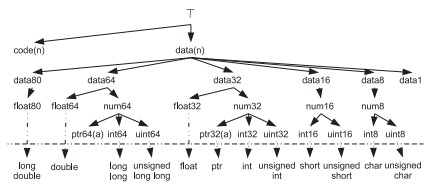
\includegraphics[width=\textwidth]{./figures/ariste-type-lattice.png}
    \caption{Ariste type lattice [][]}
    \label{fig:ariste-type-lattice}
\end{figure}

A \emph{primitive type lattice} [] is used to hierarchially relate primitive data types based on their metatype, size, and signedness (if applicable). More general types are located higher in the lattice while more specific types are located closer to the leaves. A type lattice may be used to determine whether two primitive data types are equivalent or share a common parent type.

% [Figure: Subset relationship example(s)]

We next define a \emph{subset} relationship between two data types. For a given complex data type X and another data type Y with a given offset (possibly 0) between the location of X and Y in memory, Y is considered a \emph{subset} type of X if Y is equivalent to a "portion" of X, consistent with the offset between X and Y. For example, if X is an array, any sub-array or element of X such that elements are aligned and the element types are equivalent to X is considered a subset of X. If X is a struct or union, any sub-struct or member with proper alignment and equal constituent elements is considered a subset of X.

\subsubsection{Comparison Logic}

Suppose we have two \emph{DataType} objects X (ground truth) and Y (decompiler) with offset k from the start of X to the start of Y. The goal is to compute the \emph{data type comparison level} for the given comparison. The possible values for the comparison level are as follows, from lowest equality to highest equality:

* \emph{NO\_MATCH}: No relationship could be found between X and Y.
* \emph{SUBSET}: Y is a subset type of the complex type X.
* \emph{PRIMITIVE\_COMMON\_ANCESTOR}: In the primitive type lattice, primitive types X and Y share a common ancestor type.
* \emph{MATCH}: All properties of X and Y match including metatype, size, and subtypes (if applicable).

We first check the equality of X and Y. If X and Y are equal, we assign the \emph{MATCH} comparison code. In the case that X and Y are both primitive types, we attempt to compute their shared ancestor in the primitive type lattice. If a common ancestor could be found, we assign \emph{PRIMITIVE\_COMMON\_ANCESTOR}. If X is a complex type, we employ an algorithm to determine whether Y is a subset of X at offset k by recursively descending into constituent portions of X starting at offset k (sub-structs, sub-arrays, elements, members) and checking for equality with Y. If a subset relationship is found, we assign the \emph{SUBSET} compare level. In all other cases, we assign the \emph{NO\_MATCH} compare level.

\subsection{Variable Comparison}

There are two main contexts where variable comparison occurs. The first context is at the top level, where the set of ground-truth global variables is compared to the set of decompiler global variables. The second context for variable comparison is within the context of a function when we compare parameters or local variables between the ground-truth and the decompiler. In either case, comparing sets of variables starts with the decomposition of each \emph{Variable} object from the DSL into a set of \emph{Varnode} objects in our extended DSL.

A \emph{Varnode} ties a \emph{Variable} to a specific storage location and the range of PC addresses indicating when variable lives at that location. The varnodes for a given variable are directly computed from the variable's live ranges discussed previously. In unoptimized binaries, it is the case that a single \emph{Variable} shall decompose into a single \emph{Varnode}.

With each variable decomposed into its associated varnodes, we next partition the varnodes from each the ground-truth and the decompiler based on the "address space" in which they reside. These address spaces include the \emph{absolute} address space, the \emph{stack} address space, and the \emph{register offset} address space (for a given register). The \emph{stack} address space is a special case of the \emph{register offset} address space where the offset register is the base pointer which points to the base of the current stack frame.

For the set of varnodes in each address space, we first order them based on their offset within the address space. Next, we attempt to find overlaps between varnodes from the two sources based on their location and size. If an overlap occurs between two varnodes, we compute a data type comparison taking into account the offset between the start locations of the two varnodes. The data type comparison approach is described in the previous section.

Based on the overlap status and data type comparison of a ground-truth varnode X, one of the following \emph{varnode comparison levels} will be assigned:

\begin{itemize}
    \item \emph{NO\_MATCH}: X is not overlapped with any varnodes from the other source.
    \item \emph{OVERLAP}: X overlaps with one or more varnodes from the other space, but the data type comparisons are level \emph{NO\_MATCH}.
    \item \emph{SUBSET}: X overlaps with one or more varnodes and each of its compared varnodes has data type comparison level equal to \emph{SUBSET}. In other words, the compared varnode(s) make up a portion of X.
    \item \emph{ALIGNED}: For some varnode Y from the other source, X and Y share the same location and size in memory; however, the data types of X and Y do not match. The data types comparison could have any compare level less than \emph{MATCH}.
    \item \emph{MATCH}: For some varnode Y from the other source, X and Y share the same location and size in memory, and their data types match exactly.
\end{itemize}

\subsubsection{Decomposed Variable Comparison}

The inference of variables with complex data types including structs, arrays, and unions proves to be a major challenge for decompilers. Recognizing this, we develop an approach to compare the sets of ground truth and decompiler variables (varnodes) in their most "decomposed" forms. An analysis of this sort helps to recognize how well a decompiler infers the primitive constituent components of complex variables. Furthermore, this allows us to recognize the aggressiveness and accuracy of complex variable synthesis from more primitive components.

% [Figure: Example of "decomposing" complex varnode]
\begin{figure}[ht]
    \begin{subfigure}[ht]{0.25\textwidth}
        \centering
        \begin{Verbatim}[frame=single]
typedef struct {
    int day;
    int month;
    int year;
} Date;

typedef struct {
    char* name;
    int ssn;
    float height;
    float weight;
    Date dob;
} Person;

Person people[2];
        \end{Verbatim}
        \caption{Definition of a high-level variable}
        \label{fig:decompose-src}
    \end{subfigure}
    \hfill
    \begin{subfigure}[hb]{0.75\textwidth}
        \scalebox{0.35}[0.4]{\input{./figures/decompose.latex}}
        \caption{Decomposition of a high-level varnode into primitive components}
        \label{fig:decompose-tree}
    \end{subfigure}
    \caption{Example of high-level varnode decomposition}
    \label{fig:decompose}
\end{figure}

We first implement an approach to recursively strip away the "complex layers" of a varnode to its most primitive decomposition. This primitive decomposition produces a set of one or more primitive varnodes. For example, an array of elements is broken down into a set of its elements (decomposed recursively). A struct is broken down into a set of varnodes associated with each of its members (decomposed recursively). Unions present a special case since the members share a common, overlapping region of memory. Hence, to decompose a union, we transform it into an \emph{UNDEFINED} primitive type with the same size as the union.

We apply this primitive decomposition to each varnode in the sets of ground truth and decompiler varnodes. With the two sets of decomposed varnodes, we leverage the same variable comparison approach described previously to compare the varnodes in these sets. The resulting comparison information is treated as a separate analysis from the unaltered varnode sets.

\subsection{Function Comparison}

The first step in function comparison is to determine whether each ground-truth function is found by the decompiler. We first order the functions from each source by the start PC address of the function. Next, we attempt to match the functions from the two sources based on start address. Any functions from the ground-truth that are not matched by a decompiler function are considered "missed". Functions the are found by the decompiler but absent from the ground-truth are considered "extraneous". For any missed functions, we consider its associated parameters, local variables, and data types to also be "missed".

For each "matched" function based on start PC address, we compute and store information including the return type comparison, parameter comparisons, and local variable comparisons. These sub-comparisons leverage the data type and variable comparison techniques described previously.

\section{Quantitative Evaluation Metrics}

In this section, we define quantitative metrics for evaluating the accuracy of the a given decompiler when compared to a ground-truth source. We rely on the function, variable, and data type comparison information discussed previously to extract these metrics. In the following sub-sections, we define sets of metrics that associated with tables seen in Section \ref{sec:evaluation}.

\subsection{Functions}

This set of metrics outlines the function identification performance of the decompiler.

\begin{itemize}
    \item \emph{Ground truth functions}: The number of functions present in the ground truth program representation.
    \item \emph{Functions found}: The number of functions from the ground truth set that are identified by the decompiler.
    \item \emph{Functions missed}: The number of functions from the ground truth set that are not identified by the decompiler.
    \item \emph{Functions recovery fraction}: The fraction of ground truth functions found by the decompiler divided by the number of ground truth functions.
\end{itemize}

\subsection{Varnodes}

Recall that a \emph{Varnode} is defined to be a source-level \emph{Variable} tied to a single storage location for a range of PC addresses. In analyses of unoptimized binaries, the mapping of variables to varnodes is one to one. This set of metrics illustrates the decompiler's accuracy in recovering varnodes.

\begin{itemize}
    \item \emph{Ground truth varnodes}: The total number of varnodes present in the ground truth source. This includes varnodes associated with global and local variables from all functions.
    \item \emph{Varnodes matched @ level LEVEL}: Each ground truth varnode is associated with a \emph{varnode comparison level} (\emph{NO\_MATCH}, \emph{OVERLAP}, \emph{SUBSET}, \emph{ALIGNED}, \emph{MATCH}) during the comparison with the set of decompiler varnodes. This metric specifies the number of ground truth varnodes that are matched at the specified level.
    \item \emph{Varnodes average comparison score}: For each \emph{varnode comparison level}, we first linearly assign an integer representing the strength of the varnode comparison (\emph{NO\_MATCH} = 0, \emph{OVERLAP} = 1, \emph{SUBSET} = 2, \emph{ALIGNED} = 3, \emph{MATCH} = 4). We then normalize these scores to fall within the range zero to one. Then, for each ground truth varnode, we compute this normalized score. We take the average score over all ground truth varnodes to obtain the resulting metric. This metric approximates how well, on average, the decompiler infers the ground truth varnodes.
    \item \emph{Varnodes fraction partially recovered}: The fraction of ground truth varnodes with a match level greater than \emph{NO\_MATCH}.
    \item \emph{Varnodes fraction exactly recovered}: The fraction of ground truth varnodes with a match level equal to \emph{MATCH}.
\end{itemize}

We repeat this varnode analysis for the decomposed (primitive) set of varnodes resulting from recursively decomposing each of the high-level varnodes into its most primitive set of varnodes. We also repeat our analysis of the original set of varnodes filtered by metatype. The metatypes considered are \emph{INT}, \emph{FLOAT}, \emph{POINTER}, \emph{ARRAY}, \emph{STRUCT}, and \emph{UNION}. Lastly, we repeat the analysis of the decomposed varnodes when filtered by metatype. For this metatype analysis over the decomposed varnodes, we only consider the primitive metatypes \emph{INT}, \emph{FLOAT}, and \emph{POINTER} since the varnodes are guaranteed to be primitive.

\subsection{Data Bytes}

These metrics look at the total number of data bytes from all variables recovered by the decompiler when compared to the ground truth source.

\begin{itemize}
    \item \emph{Ground truth data bytes}: The total number of data bytes captured from the ground truth source, derived from all global and local variables.
    \item \emph{Bytes found}: The total number of data bytes recovered by the decompiler that overlap with data bytes found in the ground truth.
    \item \emph{Bytes missed}: The number of data bytes present in the ground truth that were not recovered by the decompiler.
    \item \emph{Bytes recovery fraction}: The fraction of ground truth data bytes found by the decompiler divided by the total number of ground truth bytes.
\end{itemize}

\subsection{Array Comparisons}

In this set of metrics, we aim to evaluate the accuracy of the array inference performed by the decompiler. We examine each array comparison made during the comparison of the ground truth with the decompiler and observe the discrepancies in length, size (bytes), dimensions, and element type. The following metrics are presented:

\begin{itemize}
    \item \emph{Ground truth varnodes (metatype=ARRAY)}: The number of ground truth varnodes with metatype of ARRAY.
    \item \emph{Array comparisons}: The number of array comparisons made when comparing the ground truth with the decompiler. The decompiler may infer 0 or more array varnodes for each given ground truth array varnode.
    \item \emph{Array varnodes inferred as array}: This measures how many ground truth array varnodes are compared to at least 1 decompiler-inferred array varnode.
    \item \emph{Array varnodes inferred as array fraction}: Equivalent to \emph{Array varnodes inferred as array} divided by \emph{Ground truth varnodes (metatype=ARRAY)}. This expresses the fraction of ground truth array varnodes that are associated with at least one decompiler array inference.
    \item \emph{Array length (elements) average error}: For each array comparison, we find the absolute difference in the number of elements inferred by the decompiler as compared to the ground truth. We then average these differences over all array comparisons to arrive at this metric.
    \item \emph{Array length (elements) average error ratio}: For each array comparison, we first find the absolute difference in the number of elements inferred by the decompiler as compared to the ground truth. We then divide this error by the length of the ground truth array to get the error as a ratio of the array size. The average of these ratios over all array comparisons produces this metric.
    \item \emph{Array size (bytes) average error}: This metric is similar to \emph{Array length (elements) average error} but measures the error in bytes instead of number of elements.
    \item \emph{Array size (bytes) average error ratio}: This metric is similar to \emph{Array length (elements) average error ratio} but computes the error in bytes instead of array elements.
    \item \emph{Array dimension match score}: This metric is the number of array comparisons where the decompiler inferred the correct number of dimensions divided by the total number of array comparisons.
    \item \emph{Array average element type comparison score}: Each \emph{data type comparison level} is first mapped to an integer as follows: \emph{NO\_MATCH} = 0, \emph{SUBSET} = 1, \emph{PRIMITIVE\_COMMON\_ANCESTOR} = 2, \emph{MATCH} = 3. We then normalize these values such that the range is scaled from 0 to 1. We refer to this as the \emph{data type comparison score}. Then, for each array comparison, we compute the \emph{data type comparison score} and subsequently average the scores across all array comparisons to generate this metric.
\end{itemize}

\chapter{Evaluation} \label{sec:evaluation}

To demonstrate our evaluation framework, we target the Ghidra decompiler (version 10.2). We use the GNU Core Utilities programs (version 9.1) as our set of benchmarks. For each of the benchmark programs, we evaluate the accuracy of Ghidra decompilation with the program compiled in three ways: (1) stripped, (2) standard (not stripped, no debugging symbols), and (3) DWARF debug symbols included. We use the results from each of these cases to discern how the amount of information included in the binary affects the Ghidra decompiler's inference accuracy. To limit the scope of our analysis, we only consider unoptimized binaries. We use the GCC compiler (version 11.1.0) to compile the benchmark programs. The architecture and operating system of the testing machine are x86-64 and Ubuntu Linux (version 20.04), respectively.

\section{Setup}

\begin{figure}[ht]
    \centering
    \scalebox{0.5}{
        \input{./figures/evaluation-process.latex}
    }
    \caption{Evaluation workflow}
    \label{fig:evaluation-process}
\end{figure}

Prior to evaluation, we compile the 105 Coreutils benchmark programs with three compilation configurations: (1) stripped, (2) standard (not stripped, no debugging symbols), and (3) DWARF debug symbols included. For each program, we first extract the ground truth information from the binary with DWARF symbols included via our DWARF translation module. We then use our Ghidra translation module to extract the Ghidra decompilation information from the binaries compiled under each of the compilation configurations. At this point, all program information from the DWARF and Ghidra sources are represented as \emph{ProgramInfo} objects in our DSL.

Next, for each program, we perform a comparison of the program information scraped from DWARF (from the "debug" binary including DWARF symbols) with the information obtained from the Ghidra decompilation of the programs under each of the compilation configurations. The information from these comparisons are expressed in the form of objects which contain comparison information about functions, variables, and data types compared between the DWARF and Ghidra sources.

With the comparisons computed for each program and compilation configuration, we use these comparisons to compute high-level metrics that summarize the performance of the Ghidra decompiler with respect to the given benchmarks and compilation configurations (stripped, standard, and debug).

\section{Function Recovery}

\begin{table}[t]
\centering
\caption{Summary of function recovery by compilation case}
\label{table:opts-functions-summary}
\begin{tabular}{lp{4.5cm}p{4.5cm}p{4.5cm}p{4.5cm}}
\toprule
{} &  Ground truth functions &  Functions found &  Functions missed &  Functions recovery fraction \\
\midrule
strip    &                   18139 &            18139 &                 0 &                     1.000000 \\
standard &                   18139 &            18139 &                 0 &                     1.000000 \\
debug    &                   18139 &            18135 &                 4 &                     0.999779 \\
\bottomrule
\end{tabular}
\end{table}


Tables \ref{table:functions-O0-strip}, \ref{table:functions-O0}, and \ref{table:functions-O0-debug} in the appendix present function recovery metrics of each benchmark program under the three compilation configurations. Table \ref{table:opts-functions-summary} shows the summarization of the recovery statistics accumulated over all benchmark programs. We find that over the 18139 functions present in the ground truth, the stripped and standard compilation cases produce 100\% function recovery while the debug case fails to recover four functions, resulting in a 99.9\% recovery rate. Upon examination of Table \ref{table:functions-O0-debug}, we find that all four functions missed are from the \emph{factor} program.

To determine the cause of the missed functions, we further investigate the Ghidra decompilation of \emph{factor} and find that each of the missed functions results in a decompilation error, "Low-level Error: Unsupported data-type for ResolveUnion". This indicates that an error occurred when attempting to resolve a union data type within the decompilation of these functions. Since this error only occurs in the debug compilation case, it is clear that Ghidra's parsing and interpretation of DWARF information contributes to this error. This same union data type causing the error is successfully captured and represented in our ground truth program information and, thus, this is likely a bug within Ghidra's resolution logic.

In summary, we see that Ghidra successfully finds all functions for all compilation configurations. However, in the debug case, Ghidra's attempt to interpret and utilize DWARF information to resolve a union data type in the \emph{factor} program results in a decompiler error for four functions. This error indicates a bug in Ghidra's DWARF parsing or union resolution logic.

\section{High-Level Variable (Varnode) Recovery}

To evaluate the variable (varnode) recovery accuracy of the Ghidra decompiler, we first measure the inference performance of high-level varnodes, including varnodes with complex and aggregate types such as arrays, structs, and unions. We further measure the varnode inference accuracy by metatype to decipher which of the metatypes are most and least accurately inferred by the decompiler. This analysis is performed under each compilation configuration (stripped, standard, and debug).

\begin{table}[t]
\centering
\caption{Summary of high-level varnode recovery by compilation case}
\label{table:opts-varnodes-summary}
\begin{tabular}{lp{1.3cm}p{1.3cm}p{1.3cm}p{1.3cm}p{1.3cm}p{1.3cm}p{1.3cm}p{1.3cm}p{1.3cm}}
\toprule
{} & \rotatebox{70}{Varnodes matched @ level NO\_MATCH} & \rotatebox{70}{Varnodes matched @ level OVERLAP} & \rotatebox{70}{Varnodes matched @ level SUBSET} & \rotatebox{70}{Varnodes matched @ level ALIGNED} & \rotatebox{70}{Varnodes matched @ level MATCH} & \rotatebox{70}{Varnode comparison score [0,1]} & \rotatebox{70}{Varnodes fraction partially recovered} & \rotatebox{70}{Varnodes fraction exactly recovered} \\
\midrule
strip    &                                             139776 &                                            31280 &                                               0 &                                           231267 &                                         131593 &                                          0.586 &                                              0.738 &                                              0.246 \\
standard &                                              40187 &                                            56605 &                                               0 &                                           303527 &                                         133597 &                                          0.703 &                                              0.925 &                                              0.250 \\
debug    &                                              10547 &                                              128 &                                               0 &                                                5 &                                         523236 &                                          0.980 &                                              0.980 &                                              0.980 \\
\bottomrule
\end{tabular}
\end{table}


Tables \ref{table:varnodes-O0-strip}, \ref{table:varnodes-O0}, and \ref{table:varnodes-O0-debug} in the appendix show the inference of high-level varnodes for each benchmark compiled with each of the compilation configurations. This data is summarized in Table \ref{table:opts-varnodes-summary}. We find that Ghidra at least partially infers 97.2\%, 99.3\%, and 99.6\% and precisely infers 36.1\%, 38.6\%, and 99.7\% of high-level varnodes for each for the stripped, standard, and debug compilation cases, respectively. In addition, the varnode comparison scores for each compilation case are 0.788, 0.816, and 0.998, respectively. These metrics indicate that the standard compilation case slightly outperforms the stripped case in varnode inference while the debug compilation case results in significant improvements over both the stripped and standard cases, particularly in exact varnode recovery.

\begin{table}
\centering
\caption{Summary of high-level varnode recovery by compilation case and metatype}
\label{table:opts-varnodes-summary-metatypes}
\begin{tabular}{lp{1.43cm}p{1.10cm}p{1.10cm}p{1.10cm}p{1.10cm}p{1.10cm}p{1.10cm}p{1.10cm}p{1.10cm}p{1.10cm}}
\toprule
      &       &  Varnodes matched @ level NO MATCH &  Varnodes matched @ level OVERLAP &  Varnodes matched @ level SUBSET &  Varnodes matched @ level ALIGNED &  Varnodes matched @ level MATCH &  Varnode comparison score &  Varnode fraction partially recovered &  Varnode fraction exactly recovered \\
\midrule
\multirow{6}{*}{strip} & INT &                                 66 &                                48 &                                0 &                             12204 &                            8681 &                     0.850 &                                 0.997 &                               0.413 \\
      & FLOAT &                                  0 &                                56 &                                0 &                               113 &                              22 &                     0.632 &                                 1.000 &                               0.115 \\
      & POINTER &                                 53 &                                 4 &                                0 &                              5834 &                            3513 &                     0.839 &                                 0.994 &                               0.374 \\
      & ARRAY &                                729 &                               597 &                              565 &                                19 &                             228 &                     0.315 &                                 0.659 &                               0.107 \\
      & STRUCT &                                152 &                               955 &                              432 &                               390 &                             106 &                     0.419 &                                 0.925 &                               0.052 \\
      & UNION &                                  0 &                                 2 &                                4 &                                10 &                               0 &                     0.625 &                                 1.000 &                               0.000 \\
\cline{1-10}
\multirow{6}{*}{standard} & INT &                                 23 &                                48 &                                0 &                             12248 &                            8680 &                     0.851 &                                 0.999 &                               0.413 \\
      & FLOAT &                                  0 &                                56 &                                0 &                               113 &                              22 &                     0.632 &                                 1.000 &                               0.115 \\
      & POINTER &                                 44 &                                 4 &                                0 &                              5836 &                            3520 &                     0.840 &                                 0.995 &                               0.374 \\
      & ARRAY &                                181 &                               578 &                              352 &                                45 &                             982 &                     0.625 &                                 0.915 &                               0.459 \\
      & STRUCT &                                  1 &                               762 &                              257 &                               777 &                             238 &                     0.560 &                                 1.000 &                               0.117 \\
      & UNION &                                  0 &                                 2 &                                4 &                                10 &                               0 &                     0.625 &                                 1.000 &                               0.000 \\
\cline{1-10}
\multirow{6}{*}{debug} & INT &                                 13 &                                27 &                                0 &                                 4 &                           20955 &                     0.998 &                                 0.999 &                               0.998 \\
      & FLOAT &                                  0 &                                 0 &                                0 &                                 0 &                             191 &                     1.000 &                                 1.000 &                               1.000 \\
      & POINTER &                                  3 &                                 0 &                                0 &                                 1 &                            9400 &                     1.000 &                                 1.000 &                               1.000 \\
      & ARRAY &                                  5 &                                17 &                               24 &                                 0 &                            2092 &                     0.986 &                                 0.998 &                               0.978 \\
      & STRUCT &                                  2 &                                 8 &                                0 &                                 0 &                            2025 &                     0.996 &                                 0.999 &                               0.995 \\
      & UNION &                                  0 &                                 0 &                                0 &                                 2 &                              14 &                     0.969 &                                 1.000 &                               0.875 \\
\bottomrule
\end{tabular}
\end{table}


In Tables \ref{table:varnodes-metatype-INT-O0-strip}-\ref{table:varnodes-metatype-UNION-O0-strip}, \ref{table:varnodes-metatype-INT-O0}-\ref{table:varnodes-metatype-UNION-O0}, and \ref{table:varnodes-metatype-INT-O0-debug}-\ref{table:varnodes-metatype-UNION-O0-debug}, we show the inference performance of high-level varnodes for each benchmark, broken down by the metatype of the ground truth varnodes, and for all compilation configurations. We summarize this information in Table \ref{table:opts-varnodes-summary-metatypes}. From the stripped and standard compilation cases, we observe that varnodes with metatype \emph{INT} are most accurately recovered when considering varnode comparison score, fraction partially recovered, and fraction exactly recovered. In the stripped case, the inference of \emph{ARRAY} varnodes shows the worst performance with a varnode comparison score of 0.315. In the standard case, varnodes with metatype \emph{STRUCT} are least accurately recovered with a varnode comparison score of 0.560, followed closely by \emph{ARRAY} and \emph{UNION}. We see that, for both the stripped and standard compilation cases, the complex (aggregate) metatypes, \emph{ARRAY}, \emph{STRUCT}, and \emph{UNION}, show the lowest recovery accuracy with respect to varnode comparison score. Among the primitive metatypes, \emph{FLOAT} shows the worst recovery metrics for these two compilation cases.

The debug compilation case demonstrates high relative recovery accuracy across varnodes of all metatypes when compared to the stripped and standard cases. Of the primitive metatypes, varnodes of the \emph{FLOAT} metatype are perfectly recovered while varnodes of the \emph{INT} and \emph{POINTER} metatypes show exact recovery percentages of 99.8\% and 99.9\%, respectively. The complex (aggregate) metatypes, on average, display slightly lower recovery metrics than the primitive metatypes in the debug compilation case. The \emph{ARRAY} metatype reveals the worst varnode comparison score at 0.986. The \emph{UNION} metatype demonstrates the lowest exact match percentage at 87.5\%.

\section{Decomposed Variable (Varnode) Recovery}

In this section, we repeat a similar varnode recovery analysis over all varnodes; however, we first recursively decompose each varnode into a set of primitive varnodes (see Section \ref{sec:methodology}). We perform this analysis over all benchmarks for each of the three compilation cases.

\begin{table*}[t]
\centering
\caption{Summary of decomposed varnode recovery by compilation case}
\label{table*:opts-varnodes-summary-decomposed}
\begin{tabular}{lp{1.3cm}p{1.3cm}p{1.3cm}p{1.3cm}p{1.3cm}p{1.3cm}p{1.3cm}p{1.3cm}p{1.3cm}}
\toprule
{} &  Varnodes matched @ level NO\_MATCH &  Varnodes matched @ level OVERLAP &  Varnodes matched @ level SUBSET &  Varnodes matched @ level ALIGNED &  Varnodes matched @ level MATCH &  Varnode comparison score [0,1] &  Varnodes fraction partially recovered &  Varnodes fraction exactly recovered \\
\midrule
strip    &                               1000 &                              1662 &                             1001 &                             18570 &                           12550 &                           0.788 &                                  0.971 &                                0.361 \\
standard &                                249 &                              1450 &                              613 &                             19029 &                           13442 &                           0.816 &                                  0.993 &                                0.386 \\
debug    &                                 23 &                                52 &                               24 &                                 7 &                           34677 &                           0.998 &                                  0.999 &                                0.997 \\
\bottomrule
\end{tabular}
\end{table*}


Similar to the high-level varnode analysis, we show the inference of the decomposed varnodes for each benchmark and for each compilation configuration in Tables \ref{table:varnodes-decomposed-O0-strip}, \ref{table:varnodes-decomposed-O0}, and \ref{table:varnodes-decomposed-O0-debug}. Table \ref{table:opts-varnodes-summary-decomposed} summarizes this information. Naturally, we expect to see lower recovery metrics compared to the high-level varnode analysis since each complex varnode is now analyzed as a set of its constituent parts. Hence, a single "missed" high-level varnode is translated into a set of primitive varnodes, each "missed" in this analysis. We find this hypothesis to hold true across all compilation cases as each the varnode comparison score, varnodes fraction partially recovered, and varnodes fraction exactly recovered show lower values than in the high-level analysis. We see that the decomposed varnode comparison scores for the strip, standard, and debug compilation cases are 0.586, 0.703, and 0.980, respectively. The varnodes fraction partially recovered are 73.8\%, 92.5\%, and 98.0\% while the varnodes fraction exactly recovered are 24.7\%, 25.0\%, and 98.0\% across the compilation cases, respectively. Interestingly, in the stripped compilation case, we find that the number of "missed" decomposed varnodes (139937) exceeds the number of "exactly matched" decomposed varnodes (131719). This is largely due to the quantity of high-level \emph{ARRAY} and \emph{STRUCT} varnodes that are missed in the stripped case.

\begin{table}
\centering
\caption{Summary of decomposed varnode recovery by compilation case and primitive metatype}
\label{table:opts-varnodes-summary-metatypes-decomposed}
\begin{tabular}{lp{1.43cm}p{1.10cm}p{1.10cm}p{1.10cm}p{1.10cm}p{1.10cm}p{1.10cm}p{1.10cm}p{1.10cm}p{1.10cm}}
\toprule
      &         &  Varnodes matched @ level NO MATCH &  Varnodes matched @ level OVERLAP &  Varnodes matched @ level SUBSET &  Varnodes matched @ level ALIGNED &  Varnodes matched @ level MATCH &  Varnode comparison score &  Varnode fraction partially recovered &  Varnode fraction exactly recovered \\
\midrule
\multirow{3}{*}{strip} & INT &                             132910 &                             28812 &                                0 &                            217923 &                          125159 &                     0.586 &                                 0.737 &                               0.248 \\
      & FLOAT &                                 72 &                                73 &                                0 &                               103 &                              22 &                     0.435 &                                 0.733 &                               0.081 \\
      & POINTER &                               6725 &                              2057 &                                0 &                             13208 &                            6332 &                     0.591 &                                 0.763 &                               0.224 \\
\cline{1-10}
\multirow{3}{*}{standard} & INT &                              40017 &                             46846 &                                0 &                            290436 &                          127505 &                     0.707 &                                 0.921 &                               0.253 \\
      & FLOAT &                                  0 &                               145 &                                0 &                               103 &                              22 &                     0.502 &                                 1.000 &                               0.081 \\
      & POINTER &                                132 &                              9245 &                                0 &                             12955 &                            5990 &                     0.636 &                                 0.995 &                               0.211 \\
\cline{1-10}
\multirow{3}{*}{debug} & INT &                              10533 &                               124 &                                0 &                                 4 &                          494143 &                     0.979 &                                 0.979 &                               0.979 \\
      & FLOAT &                                  0 &                                 0 &                                0 &                                 0 &                             270 &                     1.000 &                                 1.000 &                               1.000 \\
      & POINTER &                                 14 &                                 2 &                                0 &                                 1 &                           28305 &                     0.999 &                                 1.000 &                               0.999 \\
\bottomrule
\end{tabular}
\end{table}


We split the decomposed varnodes by metatype and show these results in Tables \ref{table:varnodes-decomposed-metatype-INT-O0-strip}-\ref{table:varnodes-decomposed-metatype-POINTER-O0-strip}, \ref{table:varnodes-decomposed-metatype-INT-O0}-\ref{table:varnodes-decomposed-metatype-POINTER-O0}, and \ref{table:varnodes-decomposed-metatype-INT-O0-debug}-\ref{table:varnodes-decomposed-metatype-POINTER-O0-debug}. We present the summary of these results over each compilation case in Table \ref{table:opts-varnodes-summary-metatypes-decomposed}. The table shows that the stripped and standard compilation cases demostrate the poorest inference performance in terms of varnode comparison score for varnodes of metatype \emph{FLOAT}. However, we find that the percentage of "missed" \emph{INT} varnodes is worse than that of \emph{FLOAT} in the standard and debug compilation cases, and is nearly the same in the stripped case. This may be explained by the prevalence of integer (or character) arrays in the Coreutils benchmark programs when compared to other array types. Recovery accuracy of the \emph{POINTER} metatype is comparable to the \emph{INT} metatype across the three compilation cases.

\section{Data Bytes Recovery}

Following from our varnode inference analysis, we next assess the accuracy of the Ghidra decompiler with regards to the total number of data bytes recovered across all varnodes. This analysis provides an important perspective on data recovery as the size of an improperly inferred varnode may result in a wide range in the number of misinferred bytes. For example, a large array and a single character are each represented by a varnode, but the quantity of data present in the array is much greater than that of a character. Hence, it is important to capture this nuanced view of data recovery.

\begin{table}
\centering
\caption{Summary of data bytes recovery by compilation case}
\label{table:opts-bytes-summary}
\begin{tabular}{lp{1.2cm}p{1.2cm}p{1.2cm}p{1.2cm}p{1.2cm}}
\toprule
{} &  Ground truth data bytes &  Bytes found &  Bytes missed &  Bytes recovery fraction \\
\midrule
strip    &                  1183691 &       725144 &        458547 &                    0.613 \\
standard &                  1183691 &       954105 &        229586 &                    0.806 \\
debug    &                  1183691 &      1177221 &          6470 &                    0.995 \\
\bottomrule
\end{tabular}
\end{table}


In Tables \ref{table:bytes-O0-strip}, \ref{table:bytes-O0}, and \ref{table:bytes-O0-debug}, we show the data bytes recovery metrics for each of the benchmark programs under each compilation case. We summarize the data bytes recovery for each of the compilation cases in Table \ref{table:opts-bytes-summary}. We see that Ghidra recovers 61.3\%, 80.6\%, and 99.5\% of data bytes in the stripped, standard, and debug compilation cases, respectively.

\section{Array Inference Accuracy}

The last major analysis we perform targets the array inference accuracy of the Ghidra decompiler. We aim to measure metrics regarding the total number of arrays inferred, the length and size discrepancies of compared arrays, and the similarity of element types of compared arrays. We perform this analysis across the Coreutils benchmarks and for each compilation configuration, resuling in Tables \ref{table:array-comparisons-O0-strip}, \ref{table:array-comparisons-O0}, and \ref{table:array-comparisons-O0-debug} located in the appendix. This information is summarized in Table \ref{table:opts-array-comparisons-summary}, broken down by compilation configuration.

\begin{table}[t]
\centering
\caption{Summary of array recovery by compilation case}
\label{table:opts-array-comparisons-summary}
\begin{tabular}{lp{1.1cm}p{1.1cm}p{1.1cm}p{1.1cm}p{1.1cm}p{1.1cm}p{1.1cm}p{1.1cm}p{1.1cm}p{1.1cm}p{1.1cm}}
\toprule
{} & \rotatebox{90}{Ground truth array varnodes} & \rotatebox{90}{Array comparisons} & \rotatebox{90}{Array varnodes inferred as array} & \rotatebox{90}{Array varnodes inferred as array fraction} & \rotatebox{90}{Array length (elements) average error} & \rotatebox{90}{Array length (elements) average error ratio} & \rotatebox{90}{Array size (bytes) average error} & \rotatebox{90}{Array size (bytes) average error ratio} & \rotatebox{90}{Array dimension match score [0,1]} & \rotatebox{90}{Array average element type comparison score [0,1]} \\
\midrule
strip    &                                        2138 &                               823 &                                              774 &                                              0.362 &                                            134.695 &                                              2.845 &                                          458.575 &                                              0.912 &                                             0.979 &                                              0.781 \\
standard &                                        2138 &                              1579 &                                             1530 &                                              0.716 &                                            151.156 &                                              5.442 &                                          239.023 &                                              0.475 &                                             0.975 &                                              0.670 \\
debug    &                                        2138 &                              2226 &                                             2128 &                                              0.995 &                                              9.416 &                                              0.110 &                                            9.416 &                                              0.110 &                                             1.000 &                                              1.000 \\
\bottomrule
\end{tabular}
\end{table}


Across all benchmarks, there are 2138 ground truth arrays present. For each the stripped, standard, and debug compilation cases, the number of ground truth arrays recognized as arrays by the decompiler are 774 (36.2\%), 1530 (71.6\%), and 2128 (99.5\%), respectively. We see that the numbers of array comparisons for each compilation case are greater than these metrics indicating that Ghidra infers some ground truth arrays to be more than one array.

From the array comparisons, we observe that the average absolute differential in array length (number of elements) for the stripped, standard, and debug compilation cases are 134.7, 151.2, and 9.4, respectively. When scaling these errors with respect to the length of the ground truth arrays in the comparisons, the error ratios are 2.84, 5.44, and 0.11 for the compilation cases, respectively. This reveals that, in the debug case for example, the lengths of decompiler-inferred arrays are off by an average of 9.4 elements and roughly 11\% (greater or less than) of the size of the ground truth arrays they are compared to. These metrics, however, fail to capture whether the decompiler-inferred array has element types of the correct length. Thus, a similar analysis on the size (number of bytes) errors yields errors and error ratios of 458.6 (0.91), 239 (0.47), and 9.41 (0.11) for each compilation case, respectively. This, for example, shows that arrays inferred in the standard compilation case have an average absolute byte differential of 239 and a relative error of 47\% compared to the size of the ground truth array they are compared to.

In this analysis, we also capture a measure of the array dimension match score for each compilation case. This metric measures the fraction of array comparisons where the decompiler-inferred array has the same dimensionality (one-dimensional, two-dimensional, etc.) as the ground truth array. The stripped and standard compilation cases display dimensionality match ratios of greater than 97.4\%, while the debug case shows 100\% dimensionality inference accuracy.

The last portion of our array recovery analysis focuses on the element type inference accuracy of the decompiler-inferred arrays when compared to the element types of the ground truth arrays. We compute a data type comparison score between the element types from each array comparison and average these across all array comparisons derived from our benchmark programs. This data type comparison score is similar in concept to the varnode comparison score and is described in section XX. We find that decompiler-inferred arrays in the stripped, standard, and debug compilation cases show 0.781, 0.670, and 0.999 average element type comparison scores, respectively. The better performance demonstrated in the stripped case compared to the standard case appears to be a data artifact resulting from fewer array comparisons present in the stripped analysis.

\section{Debug Compilation Case Discussion}

Upon examination of our results thus far, the reader may wonder why the debug compilation case does not produce 100\% recovery for varnodes and data bytes across all benchmarks. The same DWARF debugging information used to generate the ground truth program information is also provided to the Ghidra decompiler in this case and therefore, theoretically, Ghidra should be able to precisely capture the same program information.

We manually investigate this phenomenon over our benchmark programs and find that the cause of these recovery inaccuracies stems from the Ghidra decompiler's inflexibility in expressing local variables tied to lexical scopes. We find that the Ghidra decompiler output only lists variable declarations at the top level of the function and does not support declarations of local variables within lexical scopes. Instead, Ghidra attempts to move the declaration of these scope-specific variables to the top level of the function. Often, this behavior does not negatively influence the variable recovery of the given function. However, there are cases where multiple exclusive (not overlapping or nested) lexical scopes contain variable declarations. In many of these cases, the compiler recognizes the exclusivity of the lexical scopes and assigns the scope-specific variables to shared space on the stack since the variables shall never be instantiated simultaneously. The size of the shared region allocated by the decompiler is equivalent to the size of the largest variable in the set of scope-specific variables that share the region. In essence, this is equivalent to an implicit union formed by the compiler. The DWARF debugging standard and our DSL both possess the ability to express these overlapping scope-specific variables, but the Ghidra decompiler does not. From our observations, we find that Ghidra greedily captures and declares scope-specific variables at the top level of the function based on the order in which it recovers the variables. In the debug compilation case (utilizing DWARF information), Ghidra appears to only consider the first scope-specific variable mapped to a given address on the stack based on the order of the variables in the list of debugging information entries (DIEs) parsed from DWARF. The subsequent scope-specific variables associated with the given address are simply ignored, causing Ghidra to potentially miss several varnodes and data bytes. We consider this to be a shortcoming and an area of future improvement for the Ghidra decompiler.

\chapter{Conclusion} \label{sec:conclusion}

\section{Summary of Methodology}

To develop our decompiler evaluation framework, we outline and execute the following objectives:

\begin{enumerate}
    \item Express program information such as functions, variables, data types, and addresses in a common representation.
    \item Programmatically capture a "ground truth" representation for a given program.
    \item Programmatically scrape program information from decompiler tools, namely Ghidra.
    \item Compare two program representations of the same program.
    \item Formulate quantitative metrics for evaluating the accuracy of a decompiler.
\end{enumerate}

We devise and implement a common domain-specific language (DSL) for expressing the association of high-level program information such as functions, variables, and data types, with binary-level constructs such as addresses and storage locations. With our DSL, we develop a parser for extracting DWARF debugging information from binary programs and representing this information in our DSL. This information is to be used as a ground truth source of program information in comparisons with decompiler representations. Next, we leverage the Ghidra Python API to develop a translator module, taking Ghidra decompilation output as our input and translating the information into our DSL. With our parsing modules constructed for both our ground truth and decompiler soures, we extend our DSL to support the comparison of two sources of program information parsed from a ground truth source and a decompiler source. We subsequently develop quantitative metrics for assessing and summarizing comparisons of program information sources.

\section{Summary of Results}

We utilize our developed framework to assess the recovery performance of the Ghidra decompiler (version 10.2) over the 105 GNU Core Utilities (version 9.1) benchmark programs. Using the GCC compiler (version 11.1.0), we compile the benchmarks with no optimizations under three separate compilation configurations: (1) stripped, (2) standard (not stripped, no DWARF symbols added), (3) debug (DWARF symbols included).

Our function recovery analysis reveals that Ghidra recovers 100\% of the 18139 functions across all benchmarks in the stripped and standard compilation cases. In the debug case, we find four missed functions in total, all present in the \emph{factor} benchmark program. We discover that the missed functions are all caused by a decompiler error resulting from a failure in resolving a union data type. We conclude that this is a bug in the Ghidra decompiler.

In our high-level varnode analysis, we find that the recovery accuracy of primitive (\emph{INT}, \emph{FLOAT}, \emph{POINTER}) metatypes is greater than that of the complex (aggregate) metatypes (\emph{ARRAY}, \emph{STRUCT}, \emph{UNION}) across all compilation cases. This finding follows from the fact that inferring complex varnodes involves an extra layer of speculation and inference involving the synthesis of low-level varnodes. In all compilation cases, the \emph{ARRAY} metatype displays the greatest number of "missed" varnodes.

Our decomposed (primitive) varnode analysis demonstrates that Ghidra is least effective at inferring floating-point (metatype \emph{FLOAT}) decomposed varnodes over the benchmark programs in the stripped and standard compilation cases. However, we see that Ghidra completely misses a larger fraction of decomposed varnodes with metatype \emph{INT}. This is explained by the larger incidence of integer arrays in the Coreutils benchmark programs, which are more likely to be missed or only partially recovered as demonstrated in our high-level varnode analysis. We show that decomposed varnodes of metatype \emph{POINTER} are recovered comparably to those of metatype \emph{INT}.

In our analysis of data bytes recovery summarized across all benchmarks, we find that the Ghidra decompiler shows 61.3\% recovery in the stripped compilation case, 80.6\% recovery in the standard case, and 99.5\% recovery in the debug case.

Our array inference analysis illustrates that the compilation configuration of our benchmark programs has a significant impact on both array recovery and the inference accuracy of the arrays that are recovered. We find that, for each the stripped, standard, and debug compilation cases, 36.2\%, 71.6\%, and 99.5\% of ground truth array varnodes overlap with at least one associated decompiler-inferred array varnode, respectively. We find the average size error ratio of the decompiler-inferred arrays with respect to the ground truth arrays to be 0.91, 0.47, and 0.11 for the compilation cases, respectively.

The function, variable, data bytes, and data type recovery analyses show clear recovery accuracy differentials between the three compilation cases. In general, we find that the debug case (DWARF symbols included) performs the best by a large margin, followed by the standard case which slightly outperforms the stripped case. Despite the decent recovery performance in the debug case, we seek an explanation for the decompiler still failing to capture a portion of the ground truth information, particularly varnodes and data bytes. We find that the Ghidra decompiler is limited in its ability to express overlapping stack variables gathered from non-overlapping, non-nested lexical scopes within the same parent function. This scenario arises when the compiler recoginizes the exclusivity of lexical scopes within a function and subsequently assigns scope-specific variables from these lexical scopes to the same address or region on the stack.

\section{Limitations}

The primary limitation of our framework in its current state is the lack of support for comparing and evaluating program information gathered from optimized binary programs. Our DSL supports the expression of program information from optimized binaries, but the comparison logic assumes certain properties about the program information to reduce the complexity of the analysis. Namely, we assume that each high-level variable to be associated with a single storage location in memory for the purposes of comparison. In addition, we assume that the program counter (PC) "live range" of the variable is the entire PC range of the parent function for local variables and the entire program for global variables. In optimized binaries, these assumptions do not always hold. For example, optimizations may result in a single high-level variable being stored across a combination of stack locations and registers depending on the current instruction. In essence, optimizations introduce an additional temporal dimension that drastically increases the complexity of the analysis. Each live range of each variable would need to be considered, then a set of comparison "snapshots" would need to be performed based on the overlaps of the variable live ranges. An aggregation of these "snapshot" comparisons shall then be performed in such a way to evaluate the recovery of each of the high-level variables. Our current framework is built with this type of analysis in mind, but the scope of this work only considers the case of unoptimized binaries. Future work shall include the extension of the framework to support the evaluation of optimized binaries.

Another assumption in our analysis is that only non-parameter variables with stack and absolute (global) addresses are considered for comparison. This includes heap-allocated data which must be referenced by a pointer accessible from the current function. Our language and framework support the ability to represent register and register offset locations which shall be useful in future optimized analysis.

Another limitation in this work is our exclusive support for the DWARF debugging standard for extracting ground truth program information. However, as discussed previously, our framework can easily be extended to support the implementation of parsers for other debugging formats.

Regarding decompiler evaluation, our framework excels at assessing the recovery and inference of high-level program constructs. However, our framework lacks any form of behavioral analysis. Existing work by Liu and Wang [] showcases an approach to evaluating the behavioral correctness of decompiler outputs. A full decompiler analysis shall combine our structural analysis with the behavioral analysis demonstrated by this existing work.

The final noteworthy limitation in our work is that we use our framework to assess only the Ghidra decompiler. We consider our framework to be the primary contribution of this research and therefore leave the analysis and comparison of other decompilers for future work.

\section{Future Work}

As discussed in the previous section, a major future work objective shall be to extend our framework to support optimized binaries. In addition, we shall use our framework to assess and compare the recovery performance of decompilers beyond Ghidra.

In our function recovery analysis, recall that the Ghidra decompiler fails to decompile four functions within the \emph{factor} program only in the case where DWARF debugging symbols are included. We conclude from the error messages returned that the decompilation errors for these functions result from Ghidra's inability to resolve a particular union data type present in the program. Since this error does not occur for the other compilation cases of the \emph{factor} program, we gather that the DWARF information scraped by Ghidra contributes to this error. With this observation, we recognize that a useful obfuscation strategy for binary programs may, instead of stripping all debugging symbols, be to include misleading and contradictory debugging information. Reverse engineering tools and decompilers analyzing a binary program with misleading debugging symbols included may produce incorrect outputs or potentially crash based on this erroneous information. This is certainly an area worthy of future research. In addition, the union resolution issue observed in our analysis shall be patched in the Ghidra framework.

In our assessment of the Ghidra decompiler, we observe that Ghidra does not successfully capture all ground truth variables and data bytes even in the case the DWARF debugging information is present. Upon further investigation, we discover this shortcoming is due to Ghidra's inability to express local variable declarations at the lexical scope level. Instead, Ghidra forces all local variables to be declared at the top level of the given function. This causes Ghidra to partially miss cases where the same stack address region is used by the compiler to store local variables declared in non-overlapping, non-nested lexical scopes within the same function. An area of future work shall be to modify the Ghidra decompiler to support the expression of more flexible local variable constructs that are not required to be declared at the top level of a function.

% Bibliography, default style from former template.
\global\long\def\bibname{References}
\bibliographystyle{ieee}
\bibliography{thesis-bibliography}

\begin{thebibliography}{00}
\bibitem{b1} G. Eason, B. Noble, and I. N. Sneddon, ``On certain integrals of Lipschitz-Hankel type involving products of Bessel functions,'' Phil. Trans. Roy. Soc. London, vol. A247, pp. 529--551, April 1955.
\bibitem{b2} J. Clerk Maxwell, A Treatise on Electricity and Magnetism, 3rd ed., vol. 2. Oxford: Clarendon, 1892, pp.68--73.
\bibitem{b3} I. S. Jacobs and C. P. Bean, ``Fine particles, thin films and exchange anisotropy,'' in Magnetism, vol. III, G. T. Rado and H. Suhl, Eds. New York: Academic, 1963, pp. 271--350.
\bibitem{b4} K. Elissa, ``Title of paper if known,'' unpublished.
\bibitem{b5} R. Nicole, ``Title of paper with only first word capitalized,'' J. Name Stand. Abbrev., in press.
\bibitem{b6} Y. Yorozu, M. Hirano, K. Oka, and Y. Tagawa, ``Electron spectroscopy studies on magneto-optical media and plastic substrate interface,'' IEEE Transl. J. Magn. Japan, vol. 2, pp. 740--741, August 1987 [Digests 9th Annual Conf. Magnetics Japan, p. 301, 1982].
\bibitem{b7} M. Young, The Technical Writer's Handbook. Mill Valley, CA: University Science, 1989.
\end{thebibliography}

\chapter*{Appendix}
\appendix
\small

% functions - stripped
\begin{longtable}{lp{2.40cm}p{2.40cm}p{2.40cm}p{2.40cm}p{2.40cm}}
\caption{Function recovery (compilation = stripped)}
\label{table:functions-O0-strip}\\
\toprule
{} &  Ground truth functions &  Functions found &  Functions missed &  Functions recovery fraction \\
\midrule
\endfirsthead
\caption[]{Function recovery (compilation = stripped)} \\
\toprule
{} &  Ground truth functions &  Functions found &  Functions missed &  Functions recovery fraction \\
\midrule
\endhead
\midrule
\multicolumn{5}{r}{{Continued on next page}} \\
\midrule
\endfoot

\bottomrule
\endlastfoot
{[}         &                     152 &              152 &                 0 &                        1.000 \\
b2sum     &                     148 &              148 &                 0 &                        1.000 \\
base32    &                     128 &              128 &                 0 &                        1.000 \\
base64    &                     129 &              129 &                 0 &                        1.000 \\
basename  &                     111 &              111 &                 0 &                        1.000 \\
basenc    &                     171 &              171 &                 0 &                        1.000 \\
cat       &                     124 &              124 &                 0 &                        1.000 \\
chcon     &                     247 &              247 &                 0 &                        1.000 \\
chgrp     &                     216 &              216 &                 0 &                        1.000 \\
chmod     &                     214 &              214 &                 0 &                        1.000 \\
chown     &                     218 &              218 &                 0 &                        1.000 \\
chroot    &                     125 &              125 &                 0 &                        1.000 \\
cksum     &                     246 &              246 &                 0 &                        1.000 \\
comm      &                     126 &              126 &                 0 &                        1.000 \\
cp        &                     335 &              335 &                 0 &                        1.000 \\
csplit    &                     339 &              339 &                 0 &                        1.000 \\
cut       &                     126 &              126 &                 0 &                        1.000 \\
date      &                     208 &              208 &                 0 &                        1.000 \\
dd        &                     197 &              197 &                 0 &                        1.000 \\
df        &                     266 &              266 &                 0 &                        1.000 \\
dir       &                     484 &              484 &                 0 &                        1.000 \\
dircolors &                     125 &              125 &                 0 &                        1.000 \\
dirname   &                     108 &              108 &                 0 &                        1.000 \\
du        &                     513 &              513 &                 0 &                        1.000 \\
echo      &                     105 &              105 &                 0 &                        1.000 \\
env       &                     126 &              126 &                 0 &                        1.000 \\
expand    &                     121 &              121 &                 0 &                        1.000 \\
expr      &                     323 &              323 &                 0 &                        1.000 \\
factor    &                     174 &              174 &                 0 &                        1.000 \\
false     &                     104 &              104 &                 0 &                        1.000 \\
fmt       &                     131 &              131 &                 0 &                        1.000 \\
fold      &                     116 &              116 &                 0 &                        1.000 \\
groups    &                     112 &              112 &                 0 &                        1.000 \\
head      &                     135 &              135 &                 0 &                        1.000 \\
hostid    &                     106 &              106 &                 0 &                        1.000 \\
id        &                     142 &              142 &                 0 &                        1.000 \\
join      &                     152 &              152 &                 0 &                        1.000 \\
kill      &                     112 &              112 &                 0 &                        1.000 \\
link      &                     106 &              106 &                 0 &                        1.000 \\
ln        &                     231 &              231 &                 0 &                        1.000 \\
logname   &                     106 &              106 &                 0 &                        1.000 \\
ls        &                     484 &              484 &                 0 &                        1.000 \\
md5sum    &                     132 &              132 &                 0 &                        1.000 \\
mkdir     &                     165 &              165 &                 0 &                        1.000 \\
mkfifo    &                     131 &              131 &                 0 &                        1.000 \\
mknod     &                     134 &              134 &                 0 &                        1.000 \\
mktemp    &                     120 &              120 &                 0 &                        1.000 \\
mv        &                     394 &              394 &                 0 &                        1.000 \\
nice      &                     110 &              110 &                 0 &                        1.000 \\
nl        &                     307 &              307 &                 0 &                        1.000 \\
nohup     &                     115 &              115 &                 0 &                        1.000 \\
nproc     &                     113 &              113 &                 0 &                        1.000 \\
numfmt    &                     159 &              159 &                 0 &                        1.000 \\
od        &                     172 &              172 &                 0 &                        1.000 \\
paste     &                     114 &              114 &                 0 &                        1.000 \\
pathchk   &                     110 &              110 &                 0 &                        1.000 \\
pinky     &                     124 &              124 &                 0 &                        1.000 \\
pr        &                     208 &              208 &                 0 &                        1.000 \\
printenv  &                     105 &              105 &                 0 &                        1.000 \\
printf    &                     138 &              138 &                 0 &                        1.000 \\
ptx       &                     347 &              347 &                 0 &                        1.000 \\
pwd       &                     115 &              115 &                 0 &                        1.000 \\
readlink  &                     168 &              168 &                 0 &                        1.000 \\
realpath  &                     174 &              174 &                 0 &                        1.000 \\
rm        &                     234 &              234 &                 0 &                        1.000 \\
rmdir     &                     124 &              124 &                 0 &                        1.000 \\
runcon    &                     122 &              122 &                 0 &                        1.000 \\
seq       &                     129 &              129 &                 0 &                        1.000 \\
sha1sum   &                     133 &              133 &                 0 &                        1.000 \\
sha224sum &                     140 &              140 &                 0 &                        1.000 \\
sha256sum &                     140 &              140 &                 0 &                        1.000 \\
sha384sum &                     140 &              140 &                 0 &                        1.000 \\
sha512sum &                     140 &              140 &                 0 &                        1.000 \\
shred     &                     181 &              181 &                 0 &                        1.000 \\
shuf      &                     215 &              215 &                 0 &                        1.000 \\
sleep     &                     118 &              118 &                 0 &                        1.000 \\
sort      &                     349 &              349 &                 0 &                        1.000 \\
split     &                     154 &              154 &                 0 &                        1.000 \\
stat      &                     240 &              240 &                 0 &                        1.000 \\
stdbuf    &                     135 &              135 &                 0 &                        1.000 \\
stty      &                     149 &              149 &                 0 &                        1.000 \\
sum       &                     142 &              142 &                 0 &                        1.000 \\
sync      &                     108 &              108 &                 0 &                        1.000 \\
tac       &                     310 &              310 &                 0 &                        1.000 \\
tail      &                     234 &              234 &                 0 &                        1.000 \\
tee       &                     124 &              124 &                 0 &                        1.000 \\
test      &                     147 &              147 &                 0 &                        1.000 \\
timeout   &                     130 &              130 &                 0 &                        1.000 \\
touch     &                     198 &              198 &                 0 &                        1.000 \\
tr        &                     149 &              149 &                 0 &                        1.000 \\
true      &                     104 &              104 &                 0 &                        1.000 \\
truncate  &                     114 &              114 &                 0 &                        1.000 \\
tsort     &                     125 &              125 &                 0 &                        1.000 \\
tty       &                     105 &              105 &                 0 &                        1.000 \\
uname     &                     107 &              107 &                 0 &                        1.000 \\
unexpand  &                     121 &              121 &                 0 &                        1.000 \\
uniq      &                     132 &              132 &                 0 &                        1.000 \\
unlink    &                     106 &              106 &                 0 &                        1.000 \\
uptime    &                     142 &              142 &                 0 &                        1.000 \\
users     &                     112 &              112 &                 0 &                        1.000 \\
vdir      &                     484 &              484 &                 0 &                        1.000 \\
wc        &                     152 &              152 &                 0 &                        1.000 \\
who       &                     138 &              138 &                 0 &                        1.000 \\
whoami    &                     106 &              106 &                 0 &                        1.000 \\
yes       &                     109 &              109 &                 0 &                        1.000 \\
\end{longtable}

% functions - standard
\begin{longtable}{lp{4.5cm}p{4.5cm}p{4.5cm}p{4.5cm}}
\caption{Function recovery (compilation = standard)}
\label{table:functions-O0}\\
\toprule
{} &  Ground truth functions &  Functions found &  Functions missed &  Functions recovery fraction \\
\midrule
\endfirsthead
\caption[]{Function recovery (compilation = standard)} \\
\toprule
{} &  Ground truth functions &  Functions found &  Functions missed &  Functions recovery fraction \\
\midrule
\endhead
\midrule
\multicolumn{5}{r}{{Continued on next page}} \\
\midrule
\endfoot

\bottomrule
\endlastfoot
{[}         &                     152 &              152 &                 0 &                        1.000 \\
b2sum     &                     148 &              148 &                 0 &                        1.000 \\
base32    &                     128 &              128 &                 0 &                        1.000 \\
base64    &                     129 &              129 &                 0 &                        1.000 \\
basename  &                     111 &              111 &                 0 &                        1.000 \\
basenc    &                     171 &              171 &                 0 &                        1.000 \\
cat       &                     124 &              124 &                 0 &                        1.000 \\
chcon     &                     247 &              247 &                 0 &                        1.000 \\
chgrp     &                     216 &              216 &                 0 &                        1.000 \\
chmod     &                     214 &              214 &                 0 &                        1.000 \\
chown     &                     218 &              218 &                 0 &                        1.000 \\
chroot    &                     125 &              125 &                 0 &                        1.000 \\
cksum     &                     246 &              246 &                 0 &                        1.000 \\
comm      &                     126 &              126 &                 0 &                        1.000 \\
cp        &                     335 &              335 &                 0 &                        1.000 \\
csplit    &                     339 &              339 &                 0 &                        1.000 \\
cut       &                     126 &              126 &                 0 &                        1.000 \\
date      &                     208 &              208 &                 0 &                        1.000 \\
dd        &                     197 &              197 &                 0 &                        1.000 \\
df        &                     266 &              266 &                 0 &                        1.000 \\
dir       &                     484 &              484 &                 0 &                        1.000 \\
dircolors &                     125 &              125 &                 0 &                        1.000 \\
dirname   &                     108 &              108 &                 0 &                        1.000 \\
du        &                     513 &              513 &                 0 &                        1.000 \\
echo      &                     105 &              105 &                 0 &                        1.000 \\
env       &                     126 &              126 &                 0 &                        1.000 \\
expand    &                     121 &              121 &                 0 &                        1.000 \\
expr      &                     323 &              323 &                 0 &                        1.000 \\
factor    &                     174 &              174 &                 0 &                        1.000 \\
false     &                     104 &              104 &                 0 &                        1.000 \\
fmt       &                     131 &              131 &                 0 &                        1.000 \\
fold      &                     116 &              116 &                 0 &                        1.000 \\
groups    &                     112 &              112 &                 0 &                        1.000 \\
head      &                     135 &              135 &                 0 &                        1.000 \\
hostid    &                     106 &              106 &                 0 &                        1.000 \\
id        &                     142 &              142 &                 0 &                        1.000 \\
join      &                     152 &              152 &                 0 &                        1.000 \\
kill      &                     112 &              112 &                 0 &                        1.000 \\
link      &                     106 &              106 &                 0 &                        1.000 \\
ln        &                     231 &              231 &                 0 &                        1.000 \\
logname   &                     106 &              106 &                 0 &                        1.000 \\
ls        &                     484 &              484 &                 0 &                        1.000 \\
md5sum    &                     132 &              132 &                 0 &                        1.000 \\
mkdir     &                     165 &              165 &                 0 &                        1.000 \\
mkfifo    &                     131 &              131 &                 0 &                        1.000 \\
mknod     &                     134 &              134 &                 0 &                        1.000 \\
mktemp    &                     120 &              120 &                 0 &                        1.000 \\
mv        &                     394 &              394 &                 0 &                        1.000 \\
nice      &                     110 &              110 &                 0 &                        1.000 \\
nl        &                     307 &              307 &                 0 &                        1.000 \\
nohup     &                     115 &              115 &                 0 &                        1.000 \\
nproc     &                     113 &              113 &                 0 &                        1.000 \\
numfmt    &                     159 &              159 &                 0 &                        1.000 \\
od        &                     172 &              172 &                 0 &                        1.000 \\
paste     &                     114 &              114 &                 0 &                        1.000 \\
pathchk   &                     110 &              110 &                 0 &                        1.000 \\
pinky     &                     124 &              124 &                 0 &                        1.000 \\
pr        &                     208 &              208 &                 0 &                        1.000 \\
printenv  &                     105 &              105 &                 0 &                        1.000 \\
printf    &                     138 &              138 &                 0 &                        1.000 \\
ptx       &                     347 &              347 &                 0 &                        1.000 \\
pwd       &                     115 &              115 &                 0 &                        1.000 \\
readlink  &                     168 &              168 &                 0 &                        1.000 \\
realpath  &                     174 &              174 &                 0 &                        1.000 \\
rm        &                     234 &              234 &                 0 &                        1.000 \\
rmdir     &                     124 &              124 &                 0 &                        1.000 \\
runcon    &                     122 &              122 &                 0 &                        1.000 \\
seq       &                     129 &              129 &                 0 &                        1.000 \\
sha1sum   &                     133 &              133 &                 0 &                        1.000 \\
sha224sum &                     140 &              140 &                 0 &                        1.000 \\
sha256sum &                     140 &              140 &                 0 &                        1.000 \\
sha384sum &                     140 &              140 &                 0 &                        1.000 \\
sha512sum &                     140 &              140 &                 0 &                        1.000 \\
shred     &                     181 &              181 &                 0 &                        1.000 \\
shuf      &                     215 &              215 &                 0 &                        1.000 \\
sleep     &                     118 &              118 &                 0 &                        1.000 \\
sort      &                     349 &              349 &                 0 &                        1.000 \\
split     &                     154 &              154 &                 0 &                        1.000 \\
stat      &                     240 &              240 &                 0 &                        1.000 \\
stdbuf    &                     135 &              135 &                 0 &                        1.000 \\
stty      &                     149 &              149 &                 0 &                        1.000 \\
sum       &                     142 &              142 &                 0 &                        1.000 \\
sync      &                     108 &              108 &                 0 &                        1.000 \\
tac       &                     310 &              310 &                 0 &                        1.000 \\
tail      &                     234 &              234 &                 0 &                        1.000 \\
tee       &                     124 &              124 &                 0 &                        1.000 \\
test      &                     147 &              147 &                 0 &                        1.000 \\
timeout   &                     130 &              130 &                 0 &                        1.000 \\
touch     &                     198 &              198 &                 0 &                        1.000 \\
tr        &                     149 &              149 &                 0 &                        1.000 \\
true      &                     104 &              104 &                 0 &                        1.000 \\
truncate  &                     114 &              114 &                 0 &                        1.000 \\
tsort     &                     125 &              125 &                 0 &                        1.000 \\
tty       &                     105 &              105 &                 0 &                        1.000 \\
uname     &                     107 &              107 &                 0 &                        1.000 \\
unexpand  &                     121 &              121 &                 0 &                        1.000 \\
uniq      &                     132 &              132 &                 0 &                        1.000 \\
unlink    &                     106 &              106 &                 0 &                        1.000 \\
uptime    &                     142 &              142 &                 0 &                        1.000 \\
users     &                     112 &              112 &                 0 &                        1.000 \\
vdir      &                     484 &              484 &                 0 &                        1.000 \\
wc        &                     152 &              152 &                 0 &                        1.000 \\
who       &                     138 &              138 &                 0 &                        1.000 \\
whoami    &                     106 &              106 &                 0 &                        1.000 \\
yes       &                     109 &              109 &                 0 &                        1.000 \\
\end{longtable}

% functions - debug
\begin{longtable}{lp{2.4cm}p{2.4cm}p{2.4cm}p{2.4cm}p{2.4cm}}
\caption{Function recovery (compilation = debug)}
\label{table:functions-O0-debug}\\
\toprule
{} & \rotatebox{45}{Ground truth functions} & \rotatebox{45}{Functions found} & \rotatebox{45}{Functions missed} & \rotatebox{45}{Functions recovery fraction} \\
\midrule
\endfirsthead
\caption[]{Function recovery (compilation = debug)} \\
\toprule
{} & \rotatebox{45}{Ground truth functions} & \rotatebox{45}{Functions found} & \rotatebox{45}{Functions missed} & \rotatebox{45}{Functions recovery fraction} \\
\midrule
\endhead
\midrule
\multicolumn{5}{r}{{Continued on next page}} \\
\midrule
\endfoot

\bottomrule
\endlastfoot
{[}         &                                    152 &                             152 &                                0 &                                       1.000 \\
b2sum     &                                    148 &                             148 &                                0 &                                       1.000 \\
base32    &                                    128 &                             128 &                                0 &                                       1.000 \\
base64    &                                    129 &                             129 &                                0 &                                       1.000 \\
basename  &                                    111 &                             111 &                                0 &                                       1.000 \\
basenc    &                                    171 &                             171 &                                0 &                                       1.000 \\
cat       &                                    124 &                             124 &                                0 &                                       1.000 \\
chcon     &                                    247 &                             247 &                                0 &                                       1.000 \\
chgrp     &                                    216 &                             216 &                                0 &                                       1.000 \\
chmod     &                                    214 &                             214 &                                0 &                                       1.000 \\
chown     &                                    218 &                             218 &                                0 &                                       1.000 \\
chroot    &                                    125 &                             125 &                                0 &                                       1.000 \\
cksum     &                                    246 &                             246 &                                0 &                                       1.000 \\
comm      &                                    126 &                             126 &                                0 &                                       1.000 \\
cp        &                                    335 &                             335 &                                0 &                                       1.000 \\
csplit    &                                    339 &                             339 &                                0 &                                       1.000 \\
cut       &                                    126 &                             126 &                                0 &                                       1.000 \\
date      &                                    208 &                             208 &                                0 &                                       1.000 \\
dd        &                                    197 &                             197 &                                0 &                                       1.000 \\
df        &                                    266 &                             266 &                                0 &                                       1.000 \\
dir       &                                    484 &                             484 &                                0 &                                       1.000 \\
dircolors &                                    125 &                             125 &                                0 &                                       1.000 \\
dirname   &                                    108 &                             108 &                                0 &                                       1.000 \\
du        &                                    513 &                             513 &                                0 &                                       1.000 \\
echo      &                                    105 &                             105 &                                0 &                                       1.000 \\
env       &                                    126 &                             126 &                                0 &                                       1.000 \\
expand    &                                    121 &                             121 &                                0 &                                       1.000 \\
expr      &                                    323 &                             323 &                                0 &                                       1.000 \\
factor    &                                    174 &                             170 &                                4 &                                       0.977 \\
false     &                                    104 &                             104 &                                0 &                                       1.000 \\
fmt       &                                    131 &                             131 &                                0 &                                       1.000 \\
fold      &                                    116 &                             116 &                                0 &                                       1.000 \\
groups    &                                    112 &                             112 &                                0 &                                       1.000 \\
head      &                                    135 &                             135 &                                0 &                                       1.000 \\
hostid    &                                    106 &                             106 &                                0 &                                       1.000 \\
id        &                                    142 &                             142 &                                0 &                                       1.000 \\
join      &                                    152 &                             152 &                                0 &                                       1.000 \\
kill      &                                    112 &                             112 &                                0 &                                       1.000 \\
link      &                                    106 &                             106 &                                0 &                                       1.000 \\
ln        &                                    231 &                             231 &                                0 &                                       1.000 \\
logname   &                                    106 &                             106 &                                0 &                                       1.000 \\
ls        &                                    484 &                             484 &                                0 &                                       1.000 \\
md5sum    &                                    132 &                             132 &                                0 &                                       1.000 \\
mkdir     &                                    165 &                             165 &                                0 &                                       1.000 \\
mkfifo    &                                    131 &                             131 &                                0 &                                       1.000 \\
mknod     &                                    134 &                             134 &                                0 &                                       1.000 \\
mktemp    &                                    120 &                             120 &                                0 &                                       1.000 \\
mv        &                                    394 &                             394 &                                0 &                                       1.000 \\
nice      &                                    110 &                             110 &                                0 &                                       1.000 \\
nl        &                                    307 &                             307 &                                0 &                                       1.000 \\
nohup     &                                    115 &                             115 &                                0 &                                       1.000 \\
nproc     &                                    113 &                             113 &                                0 &                                       1.000 \\
numfmt    &                                    159 &                             159 &                                0 &                                       1.000 \\
od        &                                    172 &                             172 &                                0 &                                       1.000 \\
paste     &                                    114 &                             114 &                                0 &                                       1.000 \\
pathchk   &                                    110 &                             110 &                                0 &                                       1.000 \\
pinky     &                                    124 &                             124 &                                0 &                                       1.000 \\
pr        &                                    208 &                             208 &                                0 &                                       1.000 \\
printenv  &                                    105 &                             105 &                                0 &                                       1.000 \\
printf    &                                    138 &                             138 &                                0 &                                       1.000 \\
ptx       &                                    347 &                             347 &                                0 &                                       1.000 \\
pwd       &                                    115 &                             115 &                                0 &                                       1.000 \\
readlink  &                                    168 &                             168 &                                0 &                                       1.000 \\
realpath  &                                    174 &                             174 &                                0 &                                       1.000 \\
rm        &                                    234 &                             234 &                                0 &                                       1.000 \\
rmdir     &                                    124 &                             124 &                                0 &                                       1.000 \\
runcon    &                                    122 &                             122 &                                0 &                                       1.000 \\
seq       &                                    129 &                             129 &                                0 &                                       1.000 \\
sha1sum   &                                    133 &                             133 &                                0 &                                       1.000 \\
sha224sum &                                    140 &                             140 &                                0 &                                       1.000 \\
sha256sum &                                    140 &                             140 &                                0 &                                       1.000 \\
sha384sum &                                    140 &                             140 &                                0 &                                       1.000 \\
sha512sum &                                    140 &                             140 &                                0 &                                       1.000 \\
shred     &                                    181 &                             181 &                                0 &                                       1.000 \\
shuf      &                                    215 &                             215 &                                0 &                                       1.000 \\
sleep     &                                    118 &                             118 &                                0 &                                       1.000 \\
sort      &                                    349 &                             349 &                                0 &                                       1.000 \\
split     &                                    154 &                             154 &                                0 &                                       1.000 \\
stat      &                                    240 &                             240 &                                0 &                                       1.000 \\
stdbuf    &                                    135 &                             135 &                                0 &                                       1.000 \\
stty      &                                    149 &                             149 &                                0 &                                       1.000 \\
sum       &                                    142 &                             142 &                                0 &                                       1.000 \\
sync      &                                    108 &                             108 &                                0 &                                       1.000 \\
tac       &                                    310 &                             310 &                                0 &                                       1.000 \\
tail      &                                    234 &                             234 &                                0 &                                       1.000 \\
tee       &                                    124 &                             124 &                                0 &                                       1.000 \\
test      &                                    147 &                             147 &                                0 &                                       1.000 \\
timeout   &                                    130 &                             130 &                                0 &                                       1.000 \\
touch     &                                    198 &                             198 &                                0 &                                       1.000 \\
tr        &                                    149 &                             149 &                                0 &                                       1.000 \\
true      &                                    104 &                             104 &                                0 &                                       1.000 \\
truncate  &                                    114 &                             114 &                                0 &                                       1.000 \\
tsort     &                                    125 &                             125 &                                0 &                                       1.000 \\
tty       &                                    105 &                             105 &                                0 &                                       1.000 \\
uname     &                                    107 &                             107 &                                0 &                                       1.000 \\
unexpand  &                                    121 &                             121 &                                0 &                                       1.000 \\
uniq      &                                    132 &                             132 &                                0 &                                       1.000 \\
unlink    &                                    106 &                             106 &                                0 &                                       1.000 \\
uptime    &                                    142 &                             142 &                                0 &                                       1.000 \\
users     &                                    112 &                             112 &                                0 &                                       1.000 \\
vdir      &                                    484 &                             484 &                                0 &                                       1.000 \\
wc        &                                    152 &                             152 &                                0 &                                       1.000 \\
who       &                                    138 &                             138 &                                0 &                                       1.000 \\
whoami    &                                    106 &                             106 &                                0 &                                       1.000 \\
yes       &                                    109 &                             109 &                                0 &                                       1.000 \\
\end{longtable}



% varnodes - stripped
\begin{longtable}{lp{1.2cm}p{1.2cm}p{1.2cm}p{1.2cm}p{1.2cm}p{1.2cm}p{1.2cm}p{1.2cm}p{1.2cm}p{1.2cm}}
\caption{Varnode recovery (compilation = stripped)}
\label{table:varnodes-O0-strip}\\
\toprule
{} & \rotatebox{45}{Ground truth varnodes} & \rotatebox{45}{Varnodes matched @ level NO\_MATCH} & \rotatebox{45}{Varnodes matched @ level OVERLAP} & \rotatebox{45}{Varnodes matched @ level SUBSET} & \rotatebox{45}{Varnodes matched @ level ALIGNED} & \rotatebox{45}{Varnodes matched @ level MATCH} & \rotatebox{45}{Varnode average comparison score [0,1]} & \rotatebox{45}{Varnodes fraction partially recovered} & \rotatebox{45}{Varnodes fraction exactly recovered} \\
\midrule
\endfirsthead
\caption[]{Varnode recovery (compilation = stripped)} \\
\toprule
{} & \rotatebox{45}{Ground truth varnodes} & \rotatebox{45}{Varnodes matched @ level NO\_MATCH} & \rotatebox{45}{Varnodes matched @ level OVERLAP} & \rotatebox{45}{Varnodes matched @ level SUBSET} & \rotatebox{45}{Varnodes matched @ level ALIGNED} & \rotatebox{45}{Varnodes matched @ level MATCH} & \rotatebox{45}{Varnode average comparison score [0,1]} & \rotatebox{45}{Varnodes fraction partially recovered} & \rotatebox{45}{Varnodes fraction exactly recovered} \\
\midrule
\endhead
\midrule
\multicolumn{10}{r}{{Continued on next page}} \\
\midrule
\endfoot

\bottomrule
\endlastfoot
{[}         &                                   266 &                                                  5 &                                               20 &                                              10 &                                              125 &                                            106 &                                              0.789 &                                              0.981 &                                              0.398 \\
b2sum     &                                   237 &                                                  8 &                                                9 &                                               9 &                                              115 &                                             96 &                                              0.797 &                                              0.966 &                                              0.405 \\
base32    &                                   160 &                                                  7 &                                                7 &                                               4 &                                               79 &                                             63 &                                              0.787 &                                              0.956 &                                              0.394 \\
base64    &                                   160 &                                                  7 &                                                7 &                                               4 &                                               79 &                                             63 &                                              0.787 &                                              0.956 &                                              0.394 \\
basename  &                                   129 &                                                  5 &                                                7 &                                               4 &                                               74 &                                             39 &                                              0.762 &                                              0.961 &                                              0.302 \\
basenc    &                                   219 &                                                 14 &                                                9 &                                               4 &                                              103 &                                             89 &                                              0.779 &                                              0.936 &                                              0.406 \\
cat       &                                   164 &                                                  5 &                                                8 &                                               5 &                                               92 &                                             54 &                                              0.777 &                                              0.970 &                                              0.329 \\
chcon     &                                   363 &                                                  8 &                                               16 &                                               7 &                                              229 &                                            103 &                                              0.778 &                                              0.978 &                                              0.284 \\
chgrp     &                                   339 &                                                  8 &                                               15 &                                               9 &                                              200 &                                            107 &                                              0.782 &                                              0.976 &                                              0.316 \\
chmod     &                                   347 &                                                  9 &                                               16 &                                              11 &                                              206 &                                            105 &                                              0.775 &                                              0.974 &                                              0.303 \\
chown     &                                   359 &                                                  8 &                                               16 &                                               9 &                                              206 &                                            120 &                                              0.788 &                                              0.978 &                                              0.334 \\
chroot    &                                   198 &                                                  5 &                                                9 &                                               4 &                                               84 &                                             96 &                                              0.824 &                                              0.975 &                                              0.485 \\
cksum     &                                   678 &                                                 31 &                                               26 &                                              20 &                                              392 &                                            209 &                                              0.766 &                                              0.954 &                                              0.308 \\
comm      &                                   171 &                                                  5 &                                               13 &                                               5 &                                               99 &                                             49 &                                              0.754 &                                              0.971 &                                              0.287 \\
cp        &                                   703 &                                                 17 &                                               32 &                                              30 &                                              351 &                                            273 &                                              0.796 &                                              0.976 &                                              0.388 \\
csplit    &                                   982 &                                                 15 &                                               43 &                                              17 &                                              533 &                                            374 &                                              0.808 &                                              0.985 &                                              0.381 \\
cut       &                                   192 &                                                  7 &                                                8 &                                               4 &                                              112 &                                             61 &                                              0.776 &                                              0.964 &                                              0.318 \\
date      &                                   747 &                                                 29 &                                               40 &                                              37 &                                              383 &                                            258 &                                              0.768 &                                              0.961 &                                              0.345 \\
dd        &                                   493 &                                                 18 &                                               20 &                                              12 &                                              243 &                                            200 &                                              0.798 &                                              0.963 &                                              0.406 \\
df        &                                   640 &                                                  9 &                                               25 &                                              15 &                                              283 &                                            308 &                                              0.834 &                                              0.986 &                                              0.481 \\
dir       &                                  1031 &                                                 30 &                                               56 &                                              28 &                                              544 &                                            373 &                                              0.785 &                                              0.971 &                                              0.362 \\
dircolors &                                   190 &                                                  6 &                                                8 &                                               6 &                                              111 &                                             59 &                                              0.775 &                                              0.968 &                                              0.311 \\
dirname   &                                   125 &                                                  6 &                                                7 &                                               4 &                                               70 &                                             38 &                                              0.754 &                                              0.952 &                                              0.304 \\
du        &                                  1499 &                                                 30 &                                               56 &                                              34 &                                              824 &                                            555 &                                              0.803 &                                              0.980 &                                              0.370 \\
echo      &                                   118 &                                                  4 &                                                7 &                                               4 &                                               68 &                                             35 &                                              0.761 &                                              0.966 &                                              0.297 \\
env       &                                   201 &                                                  9 &                                               12 &                                               5 &                                               97 &                                             78 &                                              0.777 &                                              0.955 &                                              0.388 \\
expand    &                                   152 &                                                  6 &                                                8 &                                               5 &                                               87 &                                             46 &                                              0.762 &                                              0.961 &                                              0.303 \\
expr      &                                   911 &                                                 15 &                                               38 &                                              27 &                                              489 &                                            342 &                                              0.803 &                                              0.984 &                                              0.375 \\
factor    &                                   511 &                                                 31 &                                               27 &                                              24 &                                              187 &                                            242 &                                              0.785 &                                              0.939 &                                              0.474 \\
false     &                                   109 &                                                  4 &                                                7 &                                               4 &                                               63 &                                             31 &                                              0.752 &                                              0.963 &                                              0.284 \\
fmt       &                                   186 &                                                  6 &                                                8 &                                               4 &                                              107 &                                             61 &                                              0.781 &                                              0.968 &                                              0.328 \\
fold      &                                   143 &                                                  6 &                                                8 &                                               4 &                                               75 &                                             50 &                                              0.771 &                                              0.958 &                                              0.350 \\
groups    &                                   142 &                                                  6 &                                                7 &                                               4 &                                               77 &                                             48 &                                              0.771 &                                              0.958 &                                              0.338 \\
head      &                                   215 &                                                  5 &                                               15 &                                               6 &                                              113 &                                             76 &                                              0.779 &                                              0.977 &                                              0.353 \\
hostid    &                                   118 &                                                  5 &                                                7 &                                               6 &                                               69 &                                             31 &                                              0.742 &                                              0.958 &                                              0.263 \\
id        &                                   196 &                                                  8 &                                                8 &                                               4 &                                               99 &                                             77 &                                              0.792 &                                              0.959 &                                              0.393 \\
join      &                                   260 &                                                  9 &                                               12 &                                               5 &                                              145 &                                             89 &                                              0.782 &                                              0.965 &                                              0.342 \\
kill      &                                   148 &                                                  7 &                                                9 &                                               4 &                                               76 &                                             52 &                                              0.765 &                                              0.953 &                                              0.351 \\
link      &                                   117 &                                                  5 &                                                7 &                                               6 &                                               68 &                                             31 &                                              0.741 &                                              0.957 &                                              0.265 \\
ln        &                                   433 &                                                  8 &                                               17 &                                              16 &                                              230 &                                            162 &                                              0.801 &                                              0.982 &                                              0.374 \\
logname   &                                   118 &                                                  5 &                                                7 &                                               6 &                                               69 &                                             31 &                                              0.742 &                                              0.958 &                                              0.263 \\
ls        &                                  1031 &                                                 30 &                                               56 &                                              28 &                                              544 &                                            373 &                                              0.785 &                                              0.971 &                                              0.362 \\
md5sum    &                                   217 &                                                  7 &                                               13 &                                               4 &                                              117 &                                             76 &                                              0.779 &                                              0.968 &                                              0.350 \\
mkdir     &                                   306 &                                                  7 &                                               15 &                                              10 &                                              146 &                                            128 &                                              0.805 &                                              0.977 &                                              0.418 \\
mkfifo    &                                   148 &                                                  6 &                                                9 &                                               5 &                                               83 &                                             45 &                                              0.757 &                                              0.959 &                                              0.304 \\
mknod     &                                   165 &                                                  6 &                                                9 &                                               5 &                                               86 &                                             59 &                                              0.777 &                                              0.964 &                                              0.358 \\
mktemp    &                                   164 &                                                  6 &                                                8 &                                               5 &                                               91 &                                             54 &                                              0.773 &                                              0.963 &                                              0.329 \\
mv        &                                   773 &                                                 15 &                                               37 &                                              26 &                                              427 &                                            268 &                                              0.790 &                                              0.981 &                                              0.347 \\
nice      &                                   130 &                                                  5 &                                                7 &                                               4 &                                               70 &                                             44 &                                              0.771 &                                              0.962 &                                              0.338 \\
nl        &                                   896 &                                                 23 &                                               39 &                                              17 &                                              468 &                                            349 &                                              0.802 &                                              0.974 &                                              0.390 \\
nohup     &                                   162 &                                                  5 &                                                8 &                                               6 &                                              102 &                                             41 &                                              0.756 &                                              0.969 &                                              0.253 \\
nproc     &                                   139 &                                                  5 &                                                7 &                                               4 &                                               74 &                                             49 &                                              0.779 &                                              0.964 &                                              0.353 \\
numfmt    &                                   291 &                                                  9 &                                               13 &                                               9 &                                              139 &                                            121 &                                              0.801 &                                              0.969 &                                              0.416 \\
od        &                                   459 &                                                 11 &                                               27 &                                              12 &                                              205 &                                            204 &                                              0.807 &                                              0.976 &                                              0.444 \\
paste     &                                   142 &                                                  5 &                                                7 &                                               4 &                                               82 &                                             44 &                                              0.769 &                                              0.965 &                                              0.310 \\
pathchk   &                                   141 &                                                  6 &                                                8 &                                               4 &                                               84 &                                             39 &                                              0.752 &                                              0.957 &                                              0.277 \\
pinky     &                                   182 &                                                  8 &                                               12 &                                               5 &                                              106 &                                             51 &                                              0.747 &                                              0.956 &                                              0.280 \\
pr        &                                   543 &                                                 12 &                                               18 &                                              10 &                                              324 &                                            179 &                                              0.795 &                                              0.978 &                                              0.330 \\
printenv  &                                   119 &                                                  5 &                                                7 &                                               4 &                                               65 &                                             38 &                                              0.761 &                                              0.958 &                                              0.319 \\
printf    &                                   283 &                                                  6 &                                               18 &                                               8 &                                              133 &                                            118 &                                              0.799 &                                              0.979 &                                              0.417 \\
ptx       &                                  1126 &                                                 19 &                                               56 &                                              32 &                                              575 &                                            444 &                                              0.804 &                                              0.983 &                                              0.394 \\
pwd       &                                   143 &                                                  5 &                                                8 &                                               9 &                                               84 &                                             37 &                                              0.745 &                                              0.965 &                                              0.259 \\
readlink  &                                   243 &                                                  6 &                                               10 &                                               7 &                                              134 &                                             86 &                                              0.792 &                                              0.975 &                                              0.354 \\
realpath  &                                   248 &                                                  6 &                                               10 &                                               7 &                                              135 &                                             90 &                                              0.795 &                                              0.976 &                                              0.363 \\
rm        &                                   362 &                                                  9 &                                               15 &                                               9 &                                              218 &                                            111 &                                              0.781 &                                              0.975 &                                              0.307 \\
rmdir     &                                   234 &                                                  6 &                                               10 &                                               7 &                                              112 &                                             99 &                                              0.808 &                                              0.974 &                                              0.423 \\
runcon    &                                   121 &                                                  5 &                                                7 &                                               4 &                                               72 &                                             33 &                                              0.750 &                                              0.959 &                                              0.273 \\
seq       &                                   279 &                                                  8 &                                               21 &                                               8 &                                              121 &                                            121 &                                              0.792 &                                              0.971 &                                              0.434 \\
sha1sum   &                                   215 &                                                  7 &                                               10 &                                               5 &                                              113 &                                             80 &                                              0.790 &                                              0.967 &                                              0.372 \\
sha224sum &                                   225 &                                                  8 &                                               13 &                                               5 &                                              116 &                                             83 &                                              0.781 &                                              0.964 &                                              0.369 \\
sha256sum &                                   225 &                                                  8 &                                               13 &                                               5 &                                              116 &                                             83 &                                              0.781 &                                              0.964 &                                              0.369 \\
sha384sum &                                   381 &                                                  8 &                                                8 &                                               5 &                                              275 &                                             85 &                                              0.776 &                                              0.979 &                                              0.223 \\
sha512sum &                                   381 &                                                  8 &                                                8 &                                               5 &                                              275 &                                             85 &                                              0.776 &                                              0.979 &                                              0.223 \\
shred     &                                   370 &                                                  9 &                                               21 &                                               8 &                                              200 &                                            132 &                                              0.787 &                                              0.976 &                                              0.357 \\
shuf      &                                   374 &                                                  6 &                                                9 &                                               6 &                                              215 &                                            138 &                                              0.814 &                                              0.984 &                                              0.369 \\
sleep     &                                   143 &                                                  5 &                                                9 &                                               6 &                                               77 &                                             46 &                                              0.762 &                                              0.965 &                                              0.322 \\
sort      &                                   847 &                                                 22 &                                               38 &                                              18 &                                              460 &                                            309 &                                              0.794 &                                              0.974 &                                              0.365 \\
split     &                                   297 &                                                  9 &                                               14 &                                               5 &                                              153 &                                            116 &                                              0.797 &                                              0.970 &                                              0.391 \\
stat      &                                   608 &                                                 20 &                                               22 &                                              20 &                                              313 &                                            233 &                                              0.795 &                                              0.967 &                                              0.383 \\
stdbuf    &                                   267 &                                                  7 &                                               10 &                                               9 &                                              125 &                                            116 &                                              0.812 &                                              0.974 &                                              0.434 \\
stty      &                                   301 &                                                  8 &                                               16 &                                              10 &                                              132 &                                            135 &                                              0.807 &                                              0.973 &                                              0.449 \\
sum       &                                   278 &                                                  8 &                                               13 &                                               7 &                                              136 &                                            114 &                                              0.801 &                                              0.971 &                                              0.410 \\
sync      &                                   133 &                                                  5 &                                                8 &                                               4 &                                               78 &                                             38 &                                              0.756 &                                              0.962 &                                              0.286 \\
tac       &                                   920 &                                                 17 &                                               39 &                                              18 &                                              500 &                                            346 &                                              0.804 &                                              0.982 &                                              0.376 \\
tail      &                                   423 &                                                  7 &                                               25 &                                              11 &                                              215 &                                            165 &                                              0.799 &                                              0.983 &                                              0.390 \\
tee       &                                   154 &                                                  6 &                                                9 &                                               5 &                                               90 &                                             44 &                                              0.755 &                                              0.961 &                                              0.286 \\
test      &                                   260 &                                                  4 &                                               19 &                                               9 &                                              125 &                                            103 &                                              0.792 &                                              0.985 &                                              0.396 \\
timeout   &                                   175 &                                                  6 &                                               10 &                                               4 &                                               86 &                                             69 &                                              0.789 &                                              0.966 &                                              0.394 \\
touch     &                                   602 &                                                 25 &                                               37 &                                              36 &                                              298 &                                            206 &                                              0.759 &                                              0.958 &                                              0.342 \\
tr        &                                   241 &                                                  9 &                                                9 &                                               6 &                                              114 &                                            103 &                                              0.804 &                                              0.963 &                                              0.427 \\
true      &                                   109 &                                                  4 &                                                7 &                                               4 &                                               63 &                                             31 &                                              0.752 &                                              0.963 &                                              0.284 \\
truncate  &                                   145 &                                                  5 &                                                8 &                                               5 &                                               80 &                                             47 &                                              0.769 &                                              0.966 &                                              0.324 \\
tsort     &                                   162 &                                                  5 &                                               10 &                                               6 &                                               93 &                                             48 &                                              0.761 &                                              0.969 &                                              0.296 \\
tty       &                                   114 &                                                  5 &                                                7 &                                               4 &                                               66 &                                             32 &                                              0.748 &                                              0.956 &                                              0.281 \\
uname     &                                   120 &                                                  6 &                                                7 &                                               5 &                                               68 &                                             34 &                                              0.744 &                                              0.950 &                                              0.283 \\
unexpand  &                                   158 &                                                  5 &                                                7 &                                               5 &                                               89 &                                             52 &                                              0.778 &                                              0.968 &                                              0.329 \\
uniq      &                                   202 &                                                  7 &                                               10 &                                               6 &                                              112 &                                             67 &                                              0.775 &                                              0.965 &                                              0.332 \\
unlink    &                                   117 &                                                  5 &                                                7 &                                               6 &                                               68 &                                             31 &                                              0.741 &                                              0.957 &                                              0.265 \\
uptime    &                                   353 &                                                 11 &                                               12 &                                              12 &                                              210 &                                            108 &                                              0.778 &                                              0.969 &                                              0.306 \\
users     &                                   133 &                                                  5 &                                                7 &                                               6 &                                               78 &                                             37 &                                              0.754 &                                              0.962 &                                              0.278 \\
vdir      &                                  1031 &                                                 30 &                                               56 &                                              28 &                                              544 &                                            373 &                                              0.785 &                                              0.971 &                                              0.362 \\
wc        &                                   268 &                                                  8 &                                                8 &                                               8 &                                              148 &                                             96 &                                              0.795 &                                              0.970 &                                              0.358 \\
who       &                                   282 &                                                 10 &                                               10 &                                               8 &                                              138 &                                            116 &                                              0.801 &                                              0.965 &                                              0.411 \\
whoami    &                                   120 &                                                  5 &                                                7 &                                               6 &                                               71 &                                             31 &                                              0.742 &                                              0.958 &                                              0.258 \\
yes       &                                   132 &                                                  5 &                                                7 &                                               6 &                                               77 &                                             37 &                                              0.754 &                                              0.962 &                                              0.280 \\
\end{longtable}


% varnodes - stripped - INT
\begin{longtable}{lp{1.2cm}p{1.2cm}p{1.2cm}p{1.2cm}p{1.2cm}p{1.2cm}p{1.2cm}p{1.2cm}p{1.2cm}p{1.2cm}}
\caption{Varnode recovery (metatype = INT) (compilation = stripped)}
\label{table:varnodes-metatype-INT-O0-strip}\\
\toprule
{} & \rotatebox{90}{Ground truth varnodes} & \rotatebox{90}{Decompiler varnodes matched @ level NO\_MATCH} & \rotatebox{90}{Decompiler varnodes matched @ level OVERLAP} & \rotatebox{90}{Decompiler varnodes matched @ level SUBSET} & \rotatebox{90}{Decompiler varnodes matched @ level ALIGNED} & \rotatebox{90}{Decompiler varnodes matched @ level MATCH} & \rotatebox{90}{Varnode average compare score [0,1]} & \rotatebox{90}{Varnodes fraction partially recovered} & \rotatebox{90}{Varnodes fraction exactly recovered} \\
\midrule
\endfirsthead
\caption[]{Varnode recovery (metatype = INT) (compilation = stripped)} \\
\toprule
{} & \rotatebox{90}{Ground truth varnodes} & \rotatebox{90}{Decompiler varnodes matched @ level NO\_MATCH} & \rotatebox{90}{Decompiler varnodes matched @ level OVERLAP} & \rotatebox{90}{Decompiler varnodes matched @ level SUBSET} & \rotatebox{90}{Decompiler varnodes matched @ level ALIGNED} & \rotatebox{90}{Decompiler varnodes matched @ level MATCH} & \rotatebox{90}{Varnode average compare score [0,1]} & \rotatebox{90}{Varnodes fraction partially recovered} & \rotatebox{90}{Varnodes fraction exactly recovered} \\
\midrule
\endhead
\midrule
\multicolumn{10}{r}{{Continued on next page}} \\
\midrule
\endfoot

\bottomrule
\endlastfoot
{[}         &                                   157 &                                                  0 &                                                  0 &                                                  0 &                                                 83 &                                                 74 &                                              0.868 &                                              1.000 &                                              0.471 \\
b2sum     &                                   147 &                                                  0 &                                                  0 &                                                  0 &                                                 80 &                                                 67 &                                              0.864 &                                              1.000 &                                              0.456 \\
base32    &                                    96 &                                                  0 &                                                  0 &                                                  0 &                                                 51 &                                                 45 &                                              0.867 &                                              1.000 &                                              0.469 \\
base64    &                                    96 &                                                  0 &                                                  0 &                                                  0 &                                                 51 &                                                 45 &                                              0.867 &                                              1.000 &                                              0.469 \\
basename  &                                    71 &                                                  0 &                                                  0 &                                                  0 &                                                 47 &                                                 24 &                                              0.835 &                                              1.000 &                                              0.338 \\
basenc    &                                   133 &                                                  0 &                                                  1 &                                                  0 &                                                 70 &                                                 62 &                                              0.863 &                                              1.000 &                                              0.466 \\
cat       &                                   101 &                                                  0 &                                                  0 &                                                  0 &                                                 64 &                                                 37 &                                              0.842 &                                              1.000 &                                              0.366 \\
chcon     &                                   185 &                                                  0 &                                                  0 &                                                  0 &                                                124 &                                                 61 &                                              0.832 &                                              1.000 &                                              0.330 \\
chgrp     &                                   166 &                                                  0 &                                                  0 &                                                  0 &                                                103 &                                                 63 &                                              0.845 &                                              1.000 &                                              0.380 \\
chmod     &                                   176 &                                                  0 &                                                  0 &                                                  0 &                                                110 &                                                 66 &                                              0.844 &                                              1.000 &                                              0.375 \\
chown     &                                   176 &                                                  0 &                                                  0 &                                                  0 &                                                105 &                                                 71 &                                              0.851 &                                              1.000 &                                              0.403 \\
chroot    &                                   110 &                                                  0 &                                                  1 &                                                  0 &                                                 53 &                                                 56 &                                              0.873 &                                              1.000 &                                              0.509 \\
cksum     &                                   488 &                                                  2 &                                                  0 &                                                  0 &                                                329 &                                                157 &                                              0.827 &                                              0.996 &                                              0.322 \\
comm      &                                   104 &                                                  0 &                                                  0 &                                                  0 &                                                 74 &                                                 30 &                                              0.822 &                                              1.000 &                                              0.288 \\
cp        &                                   382 &                                                  2 &                                                  1 &                                                  0 &                                                206 &                                                173 &                                              0.858 &                                              0.995 &                                              0.453 \\
csplit    &                                   619 &                                                  0 &                                                  1 &                                                  0 &                                                325 &                                                293 &                                              0.868 &                                              1.000 &                                              0.473 \\
cut       &                                   124 &                                                  1 &                                                  0 &                                                  0 &                                                 80 &                                                 43 &                                              0.831 &                                              0.992 &                                              0.347 \\
date      &                                   516 &                                                  4 &                                                 10 &                                                  0 &                                                317 &                                                185 &                                              0.824 &                                              0.992 &                                              0.359 \\
dd        &                                   332 &                                                  1 &                                                  0 &                                                  0 &                                                186 &                                                145 &                                              0.857 &                                              0.997 &                                              0.437 \\
df        &                                   326 &                                                  0 &                                                  0 &                                                  0 &                                                158 &                                                168 &                                              0.879 &                                              1.000 &                                              0.515 \\
dir       &                                   615 &                                                  4 &                                                  3 &                                                  0 &                                                364 &                                                244 &                                              0.842 &                                              0.993 &                                              0.397 \\
dircolors &                                    90 &                                                  0 &                                                  0 &                                                  0 &                                                 58 &                                                 32 &                                              0.839 &                                              1.000 &                                              0.356 \\
dirname   &                                    73 &                                                  1 &                                                  0 &                                                  0 &                                                 46 &                                                 26 &                                              0.829 &                                              0.986 &                                              0.356 \\
du        &                                   931 &                                                  4 &                                                  3 &                                                  0 &                                                518 &                                                406 &                                              0.854 &                                              0.996 &                                              0.436 \\
echo      &                                    69 &                                                  0 &                                                  0 &                                                  0 &                                                 45 &                                                 24 &                                              0.837 &                                              1.000 &                                              0.348 \\
env       &                                   112 &                                                  0 &                                                  0 &                                                  0 &                                                 61 &                                                 51 &                                              0.864 &                                              1.000 &                                              0.455 \\
expand    &                                    94 &                                                  0 &                                                  0 &                                                  0 &                                                 59 &                                                 35 &                                              0.843 &                                              1.000 &                                              0.372 \\
expr      &                                   560 &                                                  0 &                                                  1 &                                                  0 &                                                286 &                                                273 &                                              0.871 &                                              1.000 &                                              0.487 \\
factor    &                                   343 &                                                 21 &                                                  2 &                                                  0 &                                                128 &                                                192 &                                              0.841 &                                              0.939 &                                              0.560 \\
false     &                                    62 &                                                  0 &                                                  0 &                                                  0 &                                                 40 &                                                 22 &                                              0.839 &                                              1.000 &                                              0.355 \\
fmt       &                                   112 &                                                  0 &                                                  0 &                                                  0 &                                                 72 &                                                 40 &                                              0.839 &                                              1.000 &                                              0.357 \\
fold      &                                    88 &                                                  0 &                                                  0 &                                                  0 &                                                 51 &                                                 37 &                                              0.855 &                                              1.000 &                                              0.420 \\
groups    &                                    81 &                                                  0 &                                                  0 &                                                  0 &                                                 51 &                                                 30 &                                              0.843 &                                              1.000 &                                              0.370 \\
head      &                                   138 &                                                  0 &                                                  0 &                                                  0 &                                                 82 &                                                 56 &                                              0.851 &                                              1.000 &                                              0.406 \\
hostid    &                                    67 &                                                  0 &                                                  0 &                                                  0 &                                                 45 &                                                 22 &                                              0.832 &                                              1.000 &                                              0.328 \\
id        &                                   112 &                                                  0 &                                                  0 &                                                  0 &                                                 69 &                                                 43 &                                              0.846 &                                              1.000 &                                              0.384 \\
join      &                                   162 &                                                  0 &                                                  0 &                                                  0 &                                                104 &                                                 58 &                                              0.840 &                                              1.000 &                                              0.358 \\
kill      &                                    88 &                                                  0 &                                                  0 &                                                  0 &                                                 52 &                                                 36 &                                              0.852 &                                              1.000 &                                              0.409 \\
link      &                                    66 &                                                  0 &                                                  0 &                                                  0 &                                                 44 &                                                 22 &                                              0.833 &                                              1.000 &                                              0.333 \\
ln        &                                   219 &                                                  0 &                                                  0 &                                                  0 &                                                125 &                                                 94 &                                              0.857 &                                              1.000 &                                              0.429 \\
logname   &                                    66 &                                                  0 &                                                  0 &                                                  0 &                                                 44 &                                                 22 &                                              0.833 &                                              1.000 &                                              0.333 \\
ls        &                                   615 &                                                  4 &                                                  3 &                                                  0 &                                                364 &                                                244 &                                              0.842 &                                              0.993 &                                              0.397 \\
md5sum    &                                   139 &                                                  0 &                                                  0 &                                                  0 &                                                 81 &                                                 58 &                                              0.854 &                                              1.000 &                                              0.417 \\
mkdir     &                                   196 &                                                  0 &                                                  0 &                                                  0 &                                                102 &                                                 94 &                                              0.870 &                                              1.000 &                                              0.480 \\
mkfifo    &                                    88 &                                                  0 &                                                  0 &                                                  0 &                                                 53 &                                                 35 &                                              0.849 &                                              1.000 &                                              0.398 \\
mknod     &                                   100 &                                                  0 &                                                  0 &                                                  0 &                                                 54 &                                                 46 &                                              0.865 &                                              1.000 &                                              0.460 \\
mktemp    &                                    96 &                                                  0 &                                                  0 &                                                  0 &                                                 60 &                                                 36 &                                              0.844 &                                              1.000 &                                              0.375 \\
mv        &                                   428 &                                                  2 &                                                  0 &                                                  0 &                                                238 &                                                188 &                                              0.856 &                                              0.995 &                                              0.439 \\
nice      &                                    77 &                                                  0 &                                                  0 &                                                  0 &                                                 47 &                                                 30 &                                              0.847 &                                              1.000 &                                              0.390 \\
nl        &                                   558 &                                                  0 &                                                  1 &                                                  0 &                                                288 &                                                269 &                                              0.870 &                                              1.000 &                                              0.482 \\
nohup     &                                    99 &                                                  0 &                                                  0 &                                                  0 &                                                 71 &                                                 28 &                                              0.821 &                                              1.000 &                                              0.283 \\
nproc     &                                    86 &                                                  0 &                                                  0 &                                                  0 &                                                 51 &                                                 35 &                                              0.852 &                                              1.000 &                                              0.407 \\
numfmt    &                                   184 &                                                  0 &                                                  0 &                                                  0 &                                                 98 &                                                 86 &                                              0.867 &                                              1.000 &                                              0.467 \\
od        &                                   294 &                                                  0 &                                                  1 &                                                  0 &                                                146 &                                                147 &                                              0.873 &                                              1.000 &                                              0.500 \\
paste     &                                    85 &                                                  0 &                                                  0 &                                                  0 &                                                 55 &                                                 30 &                                              0.838 &                                              1.000 &                                              0.353 \\
pathchk   &                                    85 &                                                  0 &                                                  0 &                                                  0 &                                                 57 &                                                 28 &                                              0.832 &                                              1.000 &                                              0.329 \\
pinky     &                                    96 &                                                  0 &                                                  0 &                                                  0 &                                                 65 &                                                 31 &                                              0.831 &                                              1.000 &                                              0.323 \\
pr        &                                   399 &                                                  4 &                                                  1 &                                                  0 &                                                258 &                                                136 &                                              0.826 &                                              0.990 &                                              0.341 \\
printenv  &                                    68 &                                                  0 &                                                  0 &                                                  0 &                                                 42 &                                                 26 &                                              0.846 &                                              1.000 &                                              0.382 \\
printf    &                                   168 &                                                  0 &                                                  2 &                                                  0 &                                                 85 &                                                 81 &                                              0.865 &                                              1.000 &                                              0.482 \\
ptx       &                                   673 &                                                  0 &                                                  1 &                                                  0 &                                                347 &                                                325 &                                              0.870 &                                              1.000 &                                              0.483 \\
pwd       &                                    75 &                                                  0 &                                                  0 &                                                  0 &                                                 50 &                                                 25 &                                              0.833 &                                              1.000 &                                              0.333 \\
readlink  &                                   111 &                                                  0 &                                                  0 &                                                  0 &                                                 69 &                                                 42 &                                              0.845 &                                              1.000 &                                              0.378 \\
realpath  &                                   111 &                                                  0 &                                                  0 &                                                  0 &                                                 65 &                                                 46 &                                              0.854 &                                              1.000 &                                              0.414 \\
rm        &                                   185 &                                                  0 &                                                  0 &                                                  0 &                                                115 &                                                 70 &                                              0.845 &                                              1.000 &                                              0.378 \\
rmdir     &                                   139 &                                                  0 &                                                  0 &                                                  0 &                                                 73 &                                                 66 &                                              0.869 &                                              1.000 &                                              0.475 \\
runcon    &                                    65 &                                                  0 &                                                  0 &                                                  0 &                                                 42 &                                                 23 &                                              0.838 &                                              1.000 &                                              0.354 \\
seq       &                                   156 &                                                  0 &                                                  0 &                                                  0 &                                                 78 &                                                 78 &                                              0.875 &                                              1.000 &                                              0.500 \\
sha1sum   &                                   138 &                                                  0 &                                                  0 &                                                  0 &                                                 78 &                                                 60 &                                              0.859 &                                              1.000 &                                              0.435 \\
sha224sum &                                   145 &                                                  0 &                                                  0 &                                                  0 &                                                 80 &                                                 65 &                                              0.862 &                                              1.000 &                                              0.448 \\
sha256sum &                                   145 &                                                  0 &                                                  0 &                                                  0 &                                                 80 &                                                 65 &                                              0.862 &                                              1.000 &                                              0.448 \\
sha384sum &                                   301 &                                                  0 &                                                  0 &                                                  0 &                                                236 &                                                 65 &                                              0.804 &                                              1.000 &                                              0.216 \\
sha512sum &                                   301 &                                                  0 &                                                  0 &                                                  0 &                                                236 &                                                 65 &                                              0.804 &                                              1.000 &                                              0.216 \\
shred     &                                   238 &                                                  0 &                                                  0 &                                                  0 &                                                140 &                                                 98 &                                              0.853 &                                              1.000 &                                              0.412 \\
shuf      &                                   210 &                                                  0 &                                                  0 &                                                  0 &                                                129 &                                                 81 &                                              0.846 &                                              1.000 &                                              0.386 \\
sleep     &                                    76 &                                                  0 &                                                  0 &                                                  0 &                                                 49 &                                                 27 &                                              0.839 &                                              1.000 &                                              0.355 \\
sort      &                                   440 &                                                  0 &                                                  0 &                                                  0 &                                                260 &                                                180 &                                              0.852 &                                              1.000 &                                              0.409 \\
split     &                                   195 &                                                  0 &                                                  0 &                                                  0 &                                                109 &                                                 86 &                                              0.860 &                                              1.000 &                                              0.441 \\
stat      &                                   392 &                                                  4 &                                                  1 &                                                  0 &                                                233 &                                                154 &                                              0.839 &                                              0.990 &                                              0.393 \\
stdbuf    &                                   156 &                                                  0 &                                                  0 &                                                  0 &                                                 80 &                                                 76 &                                              0.872 &                                              1.000 &                                              0.487 \\
stty      &                                   189 &                                                  0 &                                                  1 &                                                  0 &                                                 89 &                                                 99 &                                              0.878 &                                              1.000 &                                              0.524 \\
sum       &                                   183 &                                                  0 &                                                  0 &                                                  0 &                                                 99 &                                                 84 &                                              0.865 &                                              1.000 &                                              0.459 \\
sync      &                                    83 &                                                  0 &                                                  0 &                                                  0 &                                                 54 &                                                 29 &                                              0.837 &                                              1.000 &                                              0.349 \\
tac       &                                   584 &                                                  0 &                                                  1 &                                                  0 &                                                310 &                                                273 &                                              0.866 &                                              1.000 &                                              0.467 \\
tail      &                                   239 &                                                  0 &                                                  0 &                                                  0 &                                                141 &                                                 98 &                                              0.853 &                                              1.000 &                                              0.410 \\
tee       &                                    95 &                                                  0 &                                                  0 &                                                  0 &                                                 62 &                                                 33 &                                              0.837 &                                              1.000 &                                              0.347 \\
test      &                                   155 &                                                  0 &                                                  0 &                                                  0 &                                                 83 &                                                 72 &                                              0.866 &                                              1.000 &                                              0.465 \\
timeout   &                                    95 &                                                  0 &                                                  0 &                                                  0 &                                                 55 &                                                 40 &                                              0.855 &                                              1.000 &                                              0.421 \\
touch     &                                   396 &                                                  4 &                                                  9 &                                                  0 &                                                240 &                                                143 &                                              0.821 &                                              0.990 &                                              0.361 \\
tr        &                                   153 &                                                  0 &                                                  0 &                                                  0 &                                                 70 &                                                 83 &                                              0.886 &                                              1.000 &                                              0.542 \\
true      &                                    62 &                                                  0 &                                                  0 &                                                  0 &                                                 40 &                                                 22 &                                              0.839 &                                              1.000 &                                              0.355 \\
truncate  &                                    91 &                                                  0 &                                                  0 &                                                  0 &                                                 55 &                                                 36 &                                              0.849 &                                              1.000 &                                              0.396 \\
tsort     &                                    85 &                                                  0 &                                                  0 &                                                  0 &                                                 55 &                                                 30 &                                              0.838 &                                              1.000 &                                              0.353 \\
tty       &                                    65 &                                                  0 &                                                  0 &                                                  0 &                                                 43 &                                                 22 &                                              0.835 &                                              1.000 &                                              0.338 \\
uname     &                                    67 &                                                  0 &                                                  0 &                                                  0 &                                                 43 &                                                 24 &                                              0.840 &                                              1.000 &                                              0.358 \\
unexpand  &                                   101 &                                                  0 &                                                  0 &                                                  0 &                                                 61 &                                                 40 &                                              0.849 &                                              1.000 &                                              0.396 \\
uniq      &                                   125 &                                                  0 &                                                  0 &                                                  0 &                                                 79 &                                                 46 &                                              0.842 &                                              1.000 &                                              0.368 \\
unlink    &                                    66 &                                                  0 &                                                  0 &                                                  0 &                                                 44 &                                                 22 &                                              0.833 &                                              1.000 &                                              0.333 \\
uptime    &                                   261 &                                                  4 &                                                  1 &                                                  0 &                                                170 &                                                 86 &                                              0.819 &                                              0.985 &                                              0.330 \\
users     &                                    73 &                                                  0 &                                                  0 &                                                  0 &                                                 47 &                                                 26 &                                              0.839 &                                              1.000 &                                              0.356 \\
vdir      &                                   615 &                                                  4 &                                                  3 &                                                  0 &                                                364 &                                                244 &                                              0.842 &                                              0.993 &                                              0.397 \\
wc        &                                   148 &                                                  0 &                                                  0 &                                                  0 &                                                 90 &                                                 58 &                                              0.848 &                                              1.000 &                                              0.392 \\
who       &                                   158 &                                                  0 &                                                  0 &                                                  0 &                                                 90 &                                                 68 &                                              0.858 &                                              1.000 &                                              0.430 \\
whoami    &                                    68 &                                                  0 &                                                  0 &                                                  0 &                                                 46 &                                                 22 &                                              0.831 &                                              1.000 &                                              0.324 \\
yes       &                                    76 &                                                  0 &                                                  0 &                                                  0 &                                                 50 &                                                 26 &                                              0.836 &                                              1.000 &                                              0.342 \\
\end{longtable}

% varnodes - stripped - FLOAT
\begin{longtable}{lp{1.3cm}p{1.3cm}p{1.3cm}p{1.3cm}p{1.3cm}p{1.3cm}p{1.3cm}p{1.3cm}p{1.3cm}}
\caption{Varnode recovery (metatype = FLOAT) (compilation = stripped)}
\label{table:varnodes-metatype-FLOAT-O0-strip}\\
\toprule
{} &  Ground truth varnodes &  Decompiler varnodes matched @ level NO\_MATCH &  Decompiler varnodes matched @ level OVERLAP &  Decompiler varnodes matched @ level SUBSET &  Decompiler varnodes matched @ level ALIGNED &  Decompiler varnodes matched @ level MATCH &  Varnode average compare score [0,1] &  Varnodes fraction partially recovered &  Varnodes fraction exactly recovered \\
\midrule
\endfirsthead
\caption[]{Varnode recovery (metatype = FLOAT) (compilation = stripped)} \\
\toprule
{} &  Ground truth varnodes &  Decompiler varnodes matched @ level NO\_MATCH &  Decompiler varnodes matched @ level OVERLAP &  Decompiler varnodes matched @ level SUBSET &  Decompiler varnodes matched @ level ALIGNED &  Decompiler varnodes matched @ level MATCH &  Varnode average compare score [0,1] &  Varnodes fraction partially recovered &  Varnodes fraction exactly recovered \\
\midrule
\endhead
\midrule
\multicolumn{10}{r}{{Continued on next page}} \\
\midrule
\endfoot

\bottomrule
\endlastfoot
{[}         &                      2 &                                             0 &                                            1 &                                           0 &                                            1 &                                          0 &                                0.500 &                                  1.000 &                                0.000 \\
b2sum     &                      0 &                                             0 &                                            0 &                                           0 &                                            0 &                                          0 &                                    - &                                      - &                                    - \\
base32    &                      0 &                                             0 &                                            0 &                                           0 &                                            0 &                                          0 &                                    - &                                      - &                                    - \\
base64    &                      0 &                                             0 &                                            0 &                                           0 &                                            0 &                                          0 &                                    - &                                      - &                                    - \\
basename  &                      0 &                                             0 &                                            0 &                                           0 &                                            0 &                                          0 &                                    - &                                      - &                                    - \\
basenc    &                      0 &                                             0 &                                            0 &                                           0 &                                            0 &                                          0 &                                    - &                                      - &                                    - \\
cat       &                      0 &                                             0 &                                            0 &                                           0 &                                            0 &                                          0 &                                    - &                                      - &                                    - \\
chcon     &                      3 &                                             0 &                                            0 &                                           0 &                                            3 &                                          0 &                                0.750 &                                  1.000 &                                0.000 \\
chgrp     &                      3 &                                             0 &                                            0 &                                           0 &                                            3 &                                          0 &                                0.750 &                                  1.000 &                                0.000 \\
chmod     &                      3 &                                             0 &                                            0 &                                           0 &                                            3 &                                          0 &                                0.750 &                                  1.000 &                                0.000 \\
chown     &                      3 &                                             0 &                                            0 &                                           0 &                                            3 &                                          0 &                                0.750 &                                  1.000 &                                0.000 \\
chroot    &                      0 &                                             0 &                                            0 &                                           0 &                                            0 &                                          0 &                                    - &                                      - &                                    - \\
cksum     &                      3 &                                             0 &                                            2 &                                           0 &                                            1 &                                          0 &                                0.417 &                                  1.000 &                                0.000 \\
comm      &                      0 &                                             0 &                                            0 &                                           0 &                                            0 &                                          0 &                                    - &                                      - &                                    - \\
cp        &                      3 &                                             0 &                                            0 &                                           0 &                                            3 &                                          0 &                                0.750 &                                  1.000 &                                0.000 \\
csplit    &                      0 &                                             0 &                                            0 &                                           0 &                                            0 &                                          0 &                                    - &                                      - &                                    - \\
cut       &                      0 &                                             0 &                                            0 &                                           0 &                                            0 &                                          0 &                                    - &                                      - &                                    - \\
date      &                      2 &                                             0 &                                            1 &                                           0 &                                            1 &                                          0 &                                0.500 &                                  1.000 &                                0.000 \\
dd        &                      7 &                                             0 &                                            3 &                                           0 &                                            4 &                                          0 &                                0.536 &                                  1.000 &                                0.000 \\
df        &                     13 &                                             0 &                                            3 &                                           0 &                                            5 &                                          5 &                                0.731 &                                  1.000 &                                0.385 \\
dir       &                      6 &                                             0 &                                            2 &                                           0 &                                            4 &                                          0 &                                0.583 &                                  1.000 &                                0.000 \\
dircolors &                      0 &                                             0 &                                            0 &                                           0 &                                            0 &                                          0 &                                    - &                                      - &                                    - \\
dirname   &                      0 &                                             0 &                                            0 &                                           0 &                                            0 &                                          0 &                                    - &                                      - &                                    - \\
du        &                      6 &                                             0 &                                            2 &                                           0 &                                            4 &                                          0 &                                0.583 &                                  1.000 &                                0.000 \\
echo      &                      0 &                                             0 &                                            0 &                                           0 &                                            0 &                                          0 &                                    - &                                      - &                                    - \\
env       &                      0 &                                             0 &                                            0 &                                           0 &                                            0 &                                          0 &                                    - &                                      - &                                    - \\
expand    &                      0 &                                             0 &                                            0 &                                           0 &                                            0 &                                          0 &                                    - &                                      - &                                    - \\
expr      &                      0 &                                             0 &                                            0 &                                           0 &                                            0 &                                          0 &                                    - &                                      - &                                    - \\
factor    &                      0 &                                             0 &                                            0 &                                           0 &                                            0 &                                          0 &                                    - &                                      - &                                    - \\
false     &                      0 &                                             0 &                                            0 &                                           0 &                                            0 &                                          0 &                                    - &                                      - &                                    - \\
fmt       &                      0 &                                             0 &                                            0 &                                           0 &                                            0 &                                          0 &                                    - &                                      - &                                    - \\
fold      &                      0 &                                             0 &                                            0 &                                           0 &                                            0 &                                          0 &                                    - &                                      - &                                    - \\
groups    &                      0 &                                             0 &                                            0 &                                           0 &                                            0 &                                          0 &                                    - &                                      - &                                    - \\
head      &                      0 &                                             0 &                                            0 &                                           0 &                                            0 &                                          0 &                                    - &                                      - &                                    - \\
hostid    &                      0 &                                             0 &                                            0 &                                           0 &                                            0 &                                          0 &                                    - &                                      - &                                    - \\
id        &                      0 &                                             0 &                                            0 &                                           0 &                                            0 &                                          0 &                                    - &                                      - &                                    - \\
join      &                      0 &                                             0 &                                            0 &                                           0 &                                            0 &                                          0 &                                    - &                                      - &                                    - \\
kill      &                      0 &                                             0 &                                            0 &                                           0 &                                            0 &                                          0 &                                    - &                                      - &                                    - \\
link      &                      0 &                                             0 &                                            0 &                                           0 &                                            0 &                                          0 &                                    - &                                      - &                                    - \\
ln        &                      3 &                                             0 &                                            0 &                                           0 &                                            3 &                                          0 &                                0.750 &                                  1.000 &                                0.000 \\
logname   &                      0 &                                             0 &                                            0 &                                           0 &                                            0 &                                          0 &                                    - &                                      - &                                    - \\
ls        &                      6 &                                             0 &                                            2 &                                           0 &                                            4 &                                          0 &                                0.583 &                                  1.000 &                                0.000 \\
md5sum    &                      0 &                                             0 &                                            0 &                                           0 &                                            0 &                                          0 &                                    - &                                      - &                                    - \\
mkdir     &                      2 &                                             0 &                                            1 &                                           0 &                                            1 &                                          0 &                                0.500 &                                  1.000 &                                0.000 \\
mkfifo    &                      0 &                                             0 &                                            0 &                                           0 &                                            0 &                                          0 &                                    - &                                      - &                                    - \\
mknod     &                      0 &                                             0 &                                            0 &                                           0 &                                            0 &                                          0 &                                    - &                                      - &                                    - \\
mktemp    &                      0 &                                             0 &                                            0 &                                           0 &                                            0 &                                          0 &                                    - &                                      - &                                    - \\
mv        &                      3 &                                             0 &                                            0 &                                           0 &                                            3 &                                          0 &                                0.750 &                                  1.000 &                                0.000 \\
nice      &                      0 &                                             0 &                                            0 &                                           0 &                                            0 &                                          0 &                                    - &                                      - &                                    - \\
nl        &                      0 &                                             0 &                                            0 &                                           0 &                                            0 &                                          0 &                                    - &                                      - &                                    - \\
nohup     &                      0 &                                             0 &                                            0 &                                           0 &                                            0 &                                          0 &                                    - &                                      - &                                    - \\
nproc     &                      0 &                                             0 &                                            0 &                                           0 &                                            0 &                                          0 &                                    - &                                      - &                                    - \\
numfmt    &                      7 &                                             0 &                                            5 &                                           0 &                                            2 &                                          0 &                                0.393 &                                  1.000 &                                0.000 \\
od        &                     11 &                                             0 &                                            3 &                                           0 &                                            8 &                                          0 &                                0.614 &                                  1.000 &                                0.000 \\
paste     &                      0 &                                             0 &                                            0 &                                           0 &                                            0 &                                          0 &                                    - &                                      - &                                    - \\
pathchk   &                      0 &                                             0 &                                            0 &                                           0 &                                            0 &                                          0 &                                    - &                                      - &                                    - \\
pinky     &                      0 &                                             0 &                                            0 &                                           0 &                                            0 &                                          0 &                                    - &                                      - &                                    - \\
pr        &                      0 &                                             0 &                                            0 &                                           0 &                                            0 &                                          0 &                                    - &                                      - &                                    - \\
printenv  &                      0 &                                             0 &                                            0 &                                           0 &                                            0 &                                          0 &                                    - &                                      - &                                    - \\
printf    &                      7 &                                             0 &                                            5 &                                           0 &                                            2 &                                          0 &                                0.393 &                                  1.000 &                                0.000 \\
ptx       &                      0 &                                             0 &                                            0 &                                           0 &                                            0 &                                          0 &                                    - &                                      - &                                    - \\
pwd       &                      0 &                                             0 &                                            0 &                                           0 &                                            0 &                                          0 &                                    - &                                      - &                                    - \\
readlink  &                      3 &                                             0 &                                            0 &                                           0 &                                            3 &                                          0 &                                0.750 &                                  1.000 &                                0.000 \\
realpath  &                      3 &                                             0 &                                            0 &                                           0 &                                            3 &                                          0 &                                0.750 &                                  1.000 &                                0.000 \\
rm        &                      3 &                                             0 &                                            0 &                                           0 &                                            3 &                                          0 &                                0.750 &                                  1.000 &                                0.000 \\
rmdir     &                      2 &                                             0 &                                            1 &                                           0 &                                            1 &                                          0 &                                0.500 &                                  1.000 &                                0.000 \\
runcon    &                      0 &                                             0 &                                            0 &                                           0 &                                            0 &                                          0 &                                    - &                                      - &                                    - \\
seq       &                     10 &                                             0 &                                            9 &                                           0 &                                            1 &                                          0 &                                0.300 &                                  1.000 &                                0.000 \\
sha1sum   &                      0 &                                             0 &                                            0 &                                           0 &                                            0 &                                          0 &                                    - &                                      - &                                    - \\
sha224sum &                      0 &                                             0 &                                            0 &                                           0 &                                            0 &                                          0 &                                    - &                                      - &                                    - \\
sha256sum &                      0 &                                             0 &                                            0 &                                           0 &                                            0 &                                          0 &                                    - &                                      - &                                    - \\
sha384sum &                      0 &                                             0 &                                            0 &                                           0 &                                            0 &                                          0 &                                    - &                                      - &                                    - \\
sha512sum &                      0 &                                             0 &                                            0 &                                           0 &                                            0 &                                          0 &                                    - &                                      - &                                    - \\
shred     &                      3 &                                             0 &                                            2 &                                           0 &                                            1 &                                          0 &                                0.417 &                                  1.000 &                                0.000 \\
shuf      &                      3 &                                             0 &                                            0 &                                           0 &                                            3 &                                          0 &                                0.750 &                                  1.000 &                                0.000 \\
sleep     &                      7 &                                             0 &                                            0 &                                           0 &                                            2 &                                          5 &                                0.929 &                                  1.000 &                                0.714 \\
sort      &                     18 &                                             0 &                                            4 &                                           0 &                                           12 &                                          2 &                                0.667 &                                  1.000 &                                0.111 \\
split     &                      0 &                                             0 &                                            0 &                                           0 &                                            0 &                                          0 &                                    - &                                      - &                                    - \\
stat      &                      2 &                                             0 &                                            1 &                                           0 &                                            1 &                                          0 &                                0.500 &                                  1.000 &                                0.000 \\
stdbuf    &                      2 &                                             0 &                                            1 &                                           0 &                                            1 &                                          0 &                                0.500 &                                  1.000 &                                0.000 \\
stty      &                      2 &                                             0 &                                            1 &                                           0 &                                            1 &                                          0 &                                0.500 &                                  1.000 &                                0.000 \\
sum       &                      3 &                                             0 &                                            2 &                                           0 &                                            1 &                                          0 &                                0.417 &                                  1.000 &                                0.000 \\
sync      &                      0 &                                             0 &                                            0 &                                           0 &                                            0 &                                          0 &                                    - &                                      - &                                    - \\
tac       &                      0 &                                             0 &                                            0 &                                           0 &                                            0 &                                          0 &                                    - &                                      - &                                    - \\
tail      &                     11 &                                             0 &                                            0 &                                           0 &                                            6 &                                          5 &                                0.864 &                                  1.000 &                                0.455 \\
tee       &                      0 &                                             0 &                                            0 &                                           0 &                                            0 &                                          0 &                                    - &                                      - &                                    - \\
test      &                      2 &                                             0 &                                            1 &                                           0 &                                            1 &                                          0 &                                0.500 &                                  1.000 &                                0.000 \\
timeout   &                      8 &                                             0 &                                            0 &                                           0 &                                            4 &                                          4 &                                0.875 &                                  1.000 &                                0.500 \\
touch     &                      2 &                                             0 &                                            1 &                                           0 &                                            1 &                                          0 &                                0.500 &                                  1.000 &                                0.000 \\
tr        &                      0 &                                             0 &                                            0 &                                           0 &                                            0 &                                          0 &                                    - &                                      - &                                    - \\
true      &                      0 &                                             0 &                                            0 &                                           0 &                                            0 &                                          0 &                                    - &                                      - &                                    - \\
truncate  &                      0 &                                             0 &                                            0 &                                           0 &                                            0 &                                          0 &                                    - &                                      - &                                    - \\
tsort     &                      0 &                                             0 &                                            0 &                                           0 &                                            0 &                                          0 &                                    - &                                      - &                                    - \\
tty       &                      0 &                                             0 &                                            0 &                                           0 &                                            0 &                                          0 &                                    - &                                      - &                                    - \\
uname     &                      0 &                                             0 &                                            0 &                                           0 &                                            0 &                                          0 &                                    - &                                      - &                                    - \\
unexpand  &                      0 &                                             0 &                                            0 &                                           0 &                                            0 &                                          0 &                                    - &                                      - &                                    - \\
uniq      &                      0 &                                             0 &                                            0 &                                           0 &                                            0 &                                          0 &                                    - &                                      - &                                    - \\
unlink    &                      0 &                                             0 &                                            0 &                                           0 &                                            0 &                                          0 &                                    - &                                      - &                                    - \\
uptime    &                      2 &                                             0 &                                            0 &                                           0 &                                            1 &                                          1 &                                0.875 &                                  1.000 &                                0.500 \\
users     &                      0 &                                             0 &                                            0 &                                           0 &                                            0 &                                          0 &                                    - &                                      - &                                    - \\
vdir      &                      6 &                                             0 &                                            2 &                                           0 &                                            4 &                                          0 &                                0.583 &                                  1.000 &                                0.000 \\
wc        &                      4 &                                             0 &                                            0 &                                           0 &                                            4 &                                          0 &                                0.750 &                                  1.000 &                                0.000 \\
who       &                      2 &                                             0 &                                            1 &                                           0 &                                            1 &                                          0 &                                0.500 &                                  1.000 &                                0.000 \\
whoami    &                      0 &                                             0 &                                            0 &                                           0 &                                            0 &                                          0 &                                    - &                                      - &                                    - \\
yes       &                      0 &                                             0 &                                            0 &                                           0 &                                            0 &                                          0 &                                    - &                                      - &                                    - \\
\end{longtable}

% varnodes - stripped - POINTER
\begin{longtable}{lp{2.0cm}p{2.0cm}p{2.0cm}p{2.0cm}p{2.0cm}p{2.0cm}p{2.0cm}p{2.0cm}p{2.0cm}}
\caption{Varnode recovery (metatype = POINTER) (compilation = stripped)}
\label{table:varnodes-metatype-POINTER-O0-strip}\\
\toprule
{} &  Ground truth varnodes &  Decompiler varnodes matched @ level NO\_MATCH &  Decompiler varnodes matched @ level OVERLAP &  Decompiler varnodes matched @ level SUBSET &  Decompiler varnodes matched @ level ALIGNED &  Decompiler varnodes matched @ level MATCH &  Varnode average compare score [0,1] &  Varnodes fraction partially recovered &  Varnodes fraction exactly recovered \\
\midrule
\endfirsthead
\caption[]{Varnode recovery (metatype = POINTER) (compilation = stripped)} \\
\toprule
{} &  Ground truth varnodes &  Decompiler varnodes matched @ level NO\_MATCH &  Decompiler varnodes matched @ level OVERLAP &  Decompiler varnodes matched @ level SUBSET &  Decompiler varnodes matched @ level ALIGNED &  Decompiler varnodes matched @ level MATCH &  Varnode average compare score [0,1] &  Varnodes fraction partially recovered &  Varnodes fraction exactly recovered \\
\midrule
\endhead
\midrule
\multicolumn{10}{r}{{Continued on next page}} \\
\midrule
\endfoot

\bottomrule
\endlastfoot
{[}         &                     68 &                                             0 &                                            0 &                                           0 &                                           38 &                                         30 &                                0.860 &                                  1.000 &                                0.441 \\
b2sum     &                     56 &                                             0 &                                            0 &                                           0 &                                           32 &                                         24 &                                0.857 &                                  1.000 &                                0.429 \\
base32    &                     41 &                                             0 &                                            0 &                                           0 &                                           24 &                                         17 &                                0.854 &                                  1.000 &                                0.415 \\
base64    &                     41 &                                             0 &                                            0 &                                           0 &                                           24 &                                         17 &                                0.854 &                                  1.000 &                                0.415 \\
basename  &                     38 &                                             0 &                                            0 &                                           0 &                                           24 &                                         14 &                                0.842 &                                  1.000 &                                0.368 \\
basenc    &                     55 &                                             0 &                                            0 &                                           0 &                                           30 &                                         25 &                                0.864 &                                  1.000 &                                0.455 \\
cat       &                     41 &                                             0 &                                            0 &                                           0 &                                           25 &                                         16 &                                0.848 &                                  1.000 &                                0.390 \\
chcon     &                    134 &                                             1 &                                            0 &                                           0 &                                           93 &                                         40 &                                0.819 &                                  0.993 &                                0.299 \\
chgrp     &                    133 &                                             1 &                                            0 &                                           0 &                                           90 &                                         42 &                                0.823 &                                  0.992 &                                0.316 \\
chmod     &                    127 &                                             1 &                                            0 &                                           0 &                                           89 &                                         37 &                                0.817 &                                  0.992 &                                0.291 \\
chown     &                    142 &                                             1 &                                            0 &                                           0 &                                           94 &                                         47 &                                0.827 &                                  0.993 &                                0.331 \\
chroot    &                     67 &                                             0 &                                            0 &                                           0 &                                           28 &                                         39 &                                0.896 &                                  1.000 &                                0.582 \\
cksum     &                     99 &                                             0 &                                            0 &                                           0 &                                           56 &                                         43 &                                0.859 &                                  1.000 &                                0.434 \\
comm      &                     35 &                                             0 &                                            0 &                                           0 &                                           22 &                                         13 &                                0.843 &                                  1.000 &                                0.371 \\
cp        &                    231 &                                             0 &                                            0 &                                           0 &                                          133 &                                         98 &                                0.856 &                                  1.000 &                                0.424 \\
csplit    &                    272 &                                             6 &                                            0 &                                           0 &                                          202 &                                         64 &                                0.792 &                                  0.978 &                                0.235 \\
cut       &                     46 &                                             0 &                                            0 &                                           0 &                                           29 &                                         17 &                                0.842 &                                  1.000 &                                0.370 \\
date      &                    125 &                                             1 &                                            0 &                                           0 &                                           60 &                                         64 &                                0.872 &                                  0.992 &                                0.512 \\
dd        &                     98 &                                             0 &                                            0 &                                           0 &                                           50 &                                         48 &                                0.872 &                                  1.000 &                                0.490 \\
df        &                    239 &                                             0 &                                            0 &                                           0 &                                          110 &                                        129 &                                0.885 &                                  1.000 &                                0.540 \\
dir       &                    293 &                                             1 &                                            0 &                                           0 &                                          171 &                                        121 &                                0.851 &                                  0.997 &                                0.413 \\
dircolors &                     76 &                                             0 &                                            0 &                                           0 &                                           50 &                                         26 &                                0.836 &                                  1.000 &                                0.342 \\
dirname   &                     32 &                                             0 &                                            0 &                                           0 &                                           21 &                                         11 &                                0.836 &                                  1.000 &                                0.344 \\
du        &                    438 &                                             8 &                                            0 &                                           0 &                                          295 &                                        135 &                                0.813 &                                  0.982 &                                0.308 \\
echo      &                     30 &                                             0 &                                            0 &                                           0 &                                           20 &                                         10 &                                0.833 &                                  1.000 &                                0.333 \\
env       &                     54 &                                             0 &                                            0 &                                           0 &                                           32 &                                         22 &                                0.852 &                                  1.000 &                                0.407 \\
expand    &                     35 &                                             0 &                                            0 &                                           0 &                                           25 &                                         10 &                                0.821 &                                  1.000 &                                0.286 \\
expr      &                    259 &                                             6 &                                            0 &                                           0 &                                          197 &                                         56 &                                0.787 &                                  0.977 &                                0.216 \\
factor    &                     98 &                                             1 &                                            0 &                                           0 &                                           57 &                                         40 &                                0.844 &                                  0.990 &                                0.408 \\
false     &                     28 &                                             0 &                                            0 &                                           0 &                                           20 &                                          8 &                                0.821 &                                  1.000 &                                0.286 \\
fmt       &                     52 &                                             0 &                                            0 &                                           0 &                                           32 &                                         20 &                                0.846 &                                  1.000 &                                0.385 \\
fold      &                     33 &                                             0 &                                            0 &                                           0 &                                           21 &                                         12 &                                0.841 &                                  1.000 &                                0.364 \\
groups    &                     40 &                                             0 &                                            0 &                                           0 &                                           23 &                                         17 &                                0.856 &                                  1.000 &                                0.425 \\
head      &                     47 &                                             0 &                                            0 &                                           0 &                                           28 &                                         19 &                                0.851 &                                  1.000 &                                0.404 \\
hostid    &                     29 &                                             0 &                                            0 &                                           0 &                                           21 &                                          8 &                                0.819 &                                  1.000 &                                0.276 \\
id        &                     60 &                                             0 &                                            0 &                                           0 &                                           27 &                                         33 &                                0.887 &                                  1.000 &                                0.550 \\
join      &                     66 &                                             0 &                                            0 &                                           0 &                                           38 &                                         28 &                                0.856 &                                  1.000 &                                0.424 \\
kill      &                     36 &                                             0 &                                            0 &                                           0 &                                           21 &                                         15 &                                0.854 &                                  1.000 &                                0.417 \\
link      &                     29 &                                             0 &                                            0 &                                           0 &                                           21 &                                          8 &                                0.819 &                                  1.000 &                                0.276 \\
ln        &                    161 &                                             0 &                                            0 &                                           0 &                                           95 &                                         66 &                                0.852 &                                  1.000 &                                0.410 \\
logname   &                     30 &                                             0 &                                            0 &                                           0 &                                           22 &                                          8 &                                0.817 &                                  1.000 &                                0.267 \\
ls        &                    293 &                                             1 &                                            0 &                                           0 &                                          171 &                                        121 &                                0.851 &                                  0.997 &                                0.413 \\
md5sum    &                     50 &                                             0 &                                            0 &                                           0 &                                           33 &                                         17 &                                0.835 &                                  1.000 &                                0.340 \\
mkdir     &                     71 &                                             0 &                                            0 &                                           0 &                                           39 &                                         32 &                                0.863 &                                  1.000 &                                0.451 \\
mkfifo    &                     36 &                                             0 &                                            0 &                                           0 &                                           27 &                                          9 &                                0.812 &                                  1.000 &                                0.250 \\
mknod     &                     41 &                                             0 &                                            0 &                                           0 &                                           29 &                                         12 &                                0.823 &                                  1.000 &                                0.293 \\
mktemp    &                     44 &                                             0 &                                            0 &                                           0 &                                           28 &                                         16 &                                0.841 &                                  1.000 &                                0.364 \\
mv        &                    254 &                                             1 &                                            0 &                                           0 &                                          176 &                                         77 &                                0.823 &                                  0.996 &                                0.303 \\
nice      &                     33 &                                             0 &                                            0 &                                           0 &                                           20 &                                         13 &                                0.848 &                                  1.000 &                                0.394 \\
nl        &                    247 &                                             6 &                                            0 &                                           0 &                                          174 &                                         67 &                                0.800 &                                  0.976 &                                0.271 \\
nohup     &                     40 &                                             0 &                                            0 &                                           0 &                                           28 &                                         12 &                                0.825 &                                  1.000 &                                0.300 \\
nproc     &                     32 &                                             0 &                                            0 &                                           0 &                                           20 &                                         12 &                                0.844 &                                  1.000 &                                0.375 \\
numfmt    &                     70 &                                             0 &                                            0 &                                           0 &                                           36 &                                         34 &                                0.871 &                                  1.000 &                                0.486 \\
od        &                     93 &                                             0 &                                            0 &                                           0 &                                           40 &                                         53 &                                0.892 &                                  1.000 &                                0.570 \\
paste     &                     37 &                                             0 &                                            0 &                                           0 &                                           24 &                                         13 &                                0.838 &                                  1.000 &                                0.351 \\
pathchk   &                     33 &                                             0 &                                            0 &                                           0 &                                           23 &                                         10 &                                0.826 &                                  1.000 &                                0.303 \\
pinky     &                     57 &                                             0 &                                            0 &                                           0 &                                           38 &                                         19 &                                0.833 &                                  1.000 &                                0.333 \\
pr        &                    102 &                                             1 &                                            0 &                                           0 &                                           62 &                                         39 &                                0.838 &                                  0.990 &                                0.382 \\
printenv  &                     31 &                                             0 &                                            0 &                                           0 &                                           20 &                                         11 &                                0.839 &                                  1.000 &                                0.355 \\
printf    &                     76 &                                             0 &                                            2 &                                           0 &                                           40 &                                         34 &                                0.849 &                                  1.000 &                                0.447 \\
ptx       &                    331 &                                             6 &                                            0 &                                           0 &                                          219 &                                        106 &                                0.816 &                                  0.982 &                                0.320 \\
pwd       &                     41 &                                             0 &                                            0 &                                           0 &                                           30 &                                         11 &                                0.817 &                                  1.000 &                                0.268 \\
readlink  &                    100 &                                             0 &                                            0 &                                           0 &                                           57 &                                         43 &                                0.858 &                                  1.000 &                                0.430 \\
realpath  &                    105 &                                             0 &                                            0 &                                           0 &                                           62 &                                         43 &                                0.852 &                                  1.000 &                                0.410 \\
rm        &                    136 &                                             1 &                                            0 &                                           0 &                                           96 &                                         39 &                                0.816 &                                  0.993 &                                0.287 \\
rmdir     &                     66 &                                             0 &                                            0 &                                           0 &                                           35 &                                         31 &                                0.867 &                                  1.000 &                                0.470 \\
runcon    &                     36 &                                             0 &                                            0 &                                           0 &                                           27 &                                          9 &                                0.812 &                                  1.000 &                                0.250 \\
seq       &                     81 &                                             0 &                                            1 &                                           0 &                                           39 &                                         41 &                                0.870 &                                  1.000 &                                0.506 \\
sha1sum   &                     49 &                                             0 &                                            0 &                                           0 &                                           32 &                                         17 &                                0.837 &                                  1.000 &                                0.347 \\
sha224sum &                     50 &                                             0 &                                            0 &                                           0 &                                           33 &                                         17 &                                0.835 &                                  1.000 &                                0.340 \\
sha256sum &                     50 &                                             0 &                                            0 &                                           0 &                                           33 &                                         17 &                                0.835 &                                  1.000 &                                0.340 \\
sha384sum &                     50 &                                             0 &                                            0 &                                           0 &                                           33 &                                         17 &                                0.835 &                                  1.000 &                                0.340 \\
sha512sum &                     50 &                                             0 &                                            0 &                                           0 &                                           33 &                                         17 &                                0.835 &                                  1.000 &                                0.340 \\
shred     &                     87 &                                             0 &                                            0 &                                           0 &                                           56 &                                         31 &                                0.839 &                                  1.000 &                                0.356 \\
shuf      &                    134 &                                             0 &                                            0 &                                           0 &                                           79 &                                         55 &                                0.853 &                                  1.000 &                                0.410 \\
sleep     &                     35 &                                             0 &                                            0 &                                           0 &                                           23 &                                         12 &                                0.836 &                                  1.000 &                                0.343 \\
sort      &                    299 &                                             0 &                                            0 &                                           0 &                                          182 &                                        117 &                                0.848 &                                  1.000 &                                0.391 \\
split     &                     69 &                                             0 &                                            0 &                                           0 &                                           41 &                                         28 &                                0.851 &                                  1.000 &                                0.406 \\
stat      &                    150 &                                             1 &                                            0 &                                           0 &                                           73 &                                         76 &                                0.872 &                                  0.993 &                                0.507 \\
stdbuf    &                     79 &                                             0 &                                            0 &                                           0 &                                           41 &                                         38 &                                0.870 &                                  1.000 &                                0.481 \\
stty      &                     73 &                                             0 &                                            0 &                                           0 &                                           39 &                                         34 &                                0.866 &                                  1.000 &                                0.466 \\
sum       &                     60 &                                             0 &                                            0 &                                           0 &                                           33 &                                         27 &                                0.863 &                                  1.000 &                                0.450 \\
sync      &                     29 &                                             0 &                                            0 &                                           0 &                                           21 &                                          8 &                                0.819 &                                  1.000 &                                0.276 \\
tac       &                    250 &                                             6 &                                            0 &                                           0 &                                          184 &                                         60 &                                0.792 &                                  0.976 &                                0.240 \\
tail      &                    124 &                                             0 &                                            1 &                                           0 &                                           65 &                                         58 &                                0.863 &                                  1.000 &                                0.468 \\
tee       &                     35 &                                             0 &                                            0 &                                           0 &                                           25 &                                         10 &                                0.821 &                                  1.000 &                                0.286 \\
test      &                     67 &                                             0 &                                            0 &                                           0 &                                           38 &                                         29 &                                0.858 &                                  1.000 &                                0.433 \\
timeout   &                     41 &                                             0 &                                            0 &                                           0 &                                           23 &                                         18 &                                0.860 &                                  1.000 &                                0.439 \\
touch     &                    110 &                                             1 &                                            0 &                                           0 &                                           53 &                                         56 &                                0.870 &                                  0.991 &                                0.509 \\
tr        &                     58 &                                             0 &                                            0 &                                           0 &                                           39 &                                         19 &                                0.832 &                                  1.000 &                                0.328 \\
true      &                     28 &                                             0 &                                            0 &                                           0 &                                           20 &                                          8 &                                0.821 &                                  1.000 &                                0.286 \\
truncate  &                     32 &                                             0 &                                            0 &                                           0 &                                           22 &                                         10 &                                0.828 &                                  1.000 &                                0.312 \\
tsort     &                     52 &                                             0 &                                            0 &                                           0 &                                           35 &                                         17 &                                0.832 &                                  1.000 &                                0.327 \\
tty       &                     29 &                                             0 &                                            0 &                                           0 &                                           20 &                                          9 &                                0.828 &                                  1.000 &                                0.310 \\
uname     &                     30 &                                             0 &                                            0 &                                           0 &                                           22 &                                          8 &                                0.817 &                                  1.000 &                                0.267 \\
unexpand  &                     36 &                                             0 &                                            0 &                                           0 &                                           25 &                                         11 &                                0.826 &                                  1.000 &                                0.306 \\
uniq      &                     50 &                                             0 &                                            0 &                                           0 &                                           30 &                                         20 &                                0.850 &                                  1.000 &                                0.400 \\
unlink    &                     29 &                                             0 &                                            0 &                                           0 &                                           21 &                                          8 &                                0.819 &                                  1.000 &                                0.276 \\
uptime    &                     57 &                                             1 &                                            0 &                                           0 &                                           36 &                                         20 &                                0.825 &                                  0.982 &                                0.351 \\
users     &                     38 &                                             0 &                                            0 &                                           0 &                                           28 &                                         10 &                                0.816 &                                  1.000 &                                0.263 \\
vdir      &                    293 &                                             1 &                                            0 &                                           0 &                                          171 &                                        121 &                                0.851 &                                  0.997 &                                0.413 \\
wc        &                     84 &                                             0 &                                            0 &                                           0 &                                           52 &                                         32 &                                0.845 &                                  1.000 &                                0.381 \\
who       &                     83 &                                             0 &                                            0 &                                           0 &                                           44 &                                         39 &                                0.867 &                                  1.000 &                                0.470 \\
whoami    &                     30 &                                             0 &                                            0 &                                           0 &                                           22 &                                          8 &                                0.817 &                                  1.000 &                                0.267 \\
yes       &                     34 &                                             0 &                                            0 &                                           0 &                                           24 &                                         10 &                                0.824 &                                  1.000 &                                0.294 \\
\end{longtable}

% varnodes - stripped - ARRAY
\begin{longtable}{lp{1.2cm}p{1.2cm}p{1.2cm}p{1.2cm}p{1.2cm}p{1.2cm}p{1.2cm}p{1.2cm}p{1.2cm}p{1.2cm}}
\caption{Varnode recovery (metatype = ARRAY) (compilation = stripped)}
\label{table:varnodes-metatype-ARRAY-O0-strip}\\
\toprule
{} & \rotatebox{45}{Ground truth varnodes} & \rotatebox{45}{Decompiler varnodes matched @ level NO\_MATCH} & \rotatebox{45}{Decompiler varnodes matched @ level OVERLAP} & \rotatebox{45}{Decompiler varnodes matched @ level SUBSET} & \rotatebox{45}{Decompiler varnodes matched @ level ALIGNED} & \rotatebox{45}{Decompiler varnodes matched @ level MATCH} & \rotatebox{45}{Varnode average compare score [0,1]} & \rotatebox{45}{Varnodes fraction partially recovered} & \rotatebox{45}{Varnodes fraction exactly recovered} \\
\midrule
\endfirsthead
\caption[]{Varnode recovery (metatype = ARRAY) (compilation = stripped)} \\
\toprule
{} & \rotatebox{45}{Ground truth varnodes} & \rotatebox{45}{Decompiler varnodes matched @ level NO\_MATCH} & \rotatebox{45}{Decompiler varnodes matched @ level OVERLAP} & \rotatebox{45}{Decompiler varnodes matched @ level SUBSET} & \rotatebox{45}{Decompiler varnodes matched @ level ALIGNED} & \rotatebox{45}{Decompiler varnodes matched @ level MATCH} & \rotatebox{45}{Varnode average compare score [0,1]} & \rotatebox{45}{Varnodes fraction partially recovered} & \rotatebox{45}{Varnodes fraction exactly recovered} \\
\midrule
\endhead
\midrule
\multicolumn{10}{r}{{Continued on next page}} \\
\midrule
\endfoot

\bottomrule
\endlastfoot
{[}         &                                    15 &                                                  4 &                                                  5 &                                                  4 &                                                  0 &                                                  2 &                                              0.350 &                                              0.733 &                                              0.133 \\
b2sum     &                                    24 &                                                  7 &                                                  4 &                                                  8 &                                                  0 &                                                  5 &                                              0.417 &                                              0.708 &                                              0.208 \\
base32    &                                    12 &                                                  6 &                                                  2 &                                                  3 &                                                  0 &                                                  1 &                                              0.250 &                                              0.500 &                                              0.083 \\
base64    &                                    12 &                                                  6 &                                                  2 &                                                  3 &                                                  0 &                                                  1 &                                              0.250 &                                              0.500 &                                              0.083 \\
basename  &                                    10 &                                                  4 &                                                  2 &                                                  3 &                                                  0 &                                                  1 &                                              0.300 &                                              0.600 &                                              0.100 \\
basenc    &                                    20 &                                                 13 &                                                  2 &                                                  3 &                                                  0 &                                                  2 &                                              0.200 &                                              0.350 &                                              0.100 \\
cat       &                                    11 &                                                  4 &                                                  3 &                                                  3 &                                                  0 &                                                  1 &                                              0.295 &                                              0.636 &                                              0.091 \\
chcon     &                                    18 &                                                  4 &                                                 10 &                                                  3 &                                                  0 &                                                  1 &                                              0.278 &                                              0.778 &                                              0.056 \\
chgrp     &                                    15 &                                                  4 &                                                  7 &                                                  3 &                                                  0 &                                                  1 &                                              0.283 &                                              0.733 &                                              0.067 \\
chmod     &                                    19 &                                                  5 &                                                  8 &                                                  5 &                                                  0 &                                                  1 &                                              0.289 &                                              0.737 &                                              0.053 \\
chown     &                                    16 &                                                  4 &                                                  8 &                                                  3 &                                                  0 &                                                  1 &                                              0.281 &                                              0.750 &                                              0.062 \\
chroot    &                                    11 &                                                  4 &                                                  3 &                                                  3 &                                                  0 &                                                  1 &                                              0.295 &                                              0.636 &                                              0.091 \\
cksum     &                                    66 &                                                 28 &                                                 10 &                                                 19 &                                                  0 &                                                  9 &                                              0.318 &                                              0.576 &                                              0.136 \\
comm      &                                    22 &                                                  4 &                                                  8 &                                                  4 &                                                  0 &                                                  6 &                                              0.455 &                                              0.818 &                                              0.273 \\
cp        &                                    40 &                                                 12 &                                                 13 &                                                 11 &                                                  3 &                                                  1 &                                              0.300 &                                              0.700 &                                              0.025 \\
csplit    &                                    35 &                                                  8 &                                                 13 &                                                  6 &                                                  0 &                                                  8 &                                              0.407 &                                              0.771 &                                              0.229 \\
cut       &                                    12 &                                                  5 &                                                  3 &                                                  3 &                                                  0 &                                                  1 &                                              0.271 &                                              0.583 &                                              0.083 \\
date      &                                    63 &                                                 23 &                                                 14 &                                                 20 &                                                  0 &                                                  6 &                                              0.310 &                                              0.635 &                                              0.095 \\
dd        &                                    34 &                                                 16 &                                                  7 &                                                  8 &                                                  0 &                                                  3 &                                              0.257 &                                              0.529 &                                              0.088 \\
df        &                                    25 &                                                  7 &                                                  9 &                                                  6 &                                                  1 &                                                  2 &                                              0.320 &                                              0.720 &                                              0.080 \\
dir       &                                    71 &                                                 21 &                                                 27 &                                                 19 &                                                  1 &                                                  3 &                                              0.282 &                                              0.704 &                                              0.042 \\
dircolors &                                    13 &                                                  5 &                                                  2 &                                                  5 &                                                  0 &                                                  1 &                                              0.308 &                                              0.615 &                                              0.077 \\
dirname   &                                    10 &                                                  4 &                                                  2 &                                                  3 &                                                  0 &                                                  1 &                                              0.300 &                                              0.600 &                                              0.100 \\
du        &                                    51 &                                                 15 &                                                 16 &                                                 12 &                                                  0 &                                                  8 &                                              0.353 &                                              0.706 &                                              0.157 \\
echo      &                                     9 &                                                  3 &                                                  2 &                                                  3 &                                                  0 &                                                  1 &                                              0.333 &                                              0.667 &                                              0.111 \\
env       &                                    18 &                                                  6 &                                                  7 &                                                  3 &                                                  1 &                                                  1 &                                              0.278 &                                              0.667 &                                              0.056 \\
expand    &                                    13 &                                                  5 &                                                  3 &                                                  4 &                                                  0 &                                                  1 &                                              0.288 &                                              0.615 &                                              0.077 \\
expr      &                                    33 &                                                  8 &                                                  9 &                                                  8 &                                                  0 &                                                  8 &                                              0.432 &                                              0.758 &                                              0.242 \\
factor    &                                    37 &                                                  8 &                                                 10 &                                                 10 &                                                  0 &                                                  9 &                                              0.446 &                                              0.784 &                                              0.243 \\
false     &                                     9 &                                                  3 &                                                  2 &                                                  3 &                                                  0 &                                                  1 &                                              0.333 &                                              0.667 &                                              0.111 \\
fmt       &                                    12 &                                                  5 &                                                  3 &                                                  3 &                                                  0 &                                                  1 &                                              0.271 &                                              0.583 &                                              0.083 \\
fold      &                                    12 &                                                  5 &                                                  3 &                                                  3 &                                                  0 &                                                  1 &                                              0.271 &                                              0.583 &                                              0.083 \\
groups    &                                    11 &                                                  5 &                                                  2 &                                                  3 &                                                  0 &                                                  1 &                                              0.273 &                                              0.545 &                                              0.091 \\
head      &                                    18 &                                                  4 &                                                  9 &                                                  4 &                                                  0 &                                                  1 &                                              0.292 &                                              0.778 &                                              0.056 \\
hostid    &                                    12 &                                                  4 &                                                  2 &                                                  5 &                                                  0 &                                                  1 &                                              0.333 &                                              0.667 &                                              0.083 \\
id        &                                    14 &                                                  7 &                                                  3 &                                                  3 &                                                  0 &                                                  1 &                                              0.232 &                                              0.500 &                                              0.071 \\
join      &                                    18 &                                                  7 &                                                  5 &                                                  3 &                                                  0 &                                                  3 &                                              0.319 &                                              0.611 &                                              0.167 \\
kill      &                                    14 &                                                  6 &                                                  4 &                                                  3 &                                                  0 &                                                  1 &                                              0.250 &                                              0.571 &                                              0.071 \\
link      &                                    12 &                                                  4 &                                                  2 &                                                  5 &                                                  0 &                                                  1 &                                              0.333 &                                              0.667 &                                              0.083 \\
ln        &                                    22 &                                                  6 &                                                  7 &                                                  5 &                                                  3 &                                                  1 &                                              0.341 &                                              0.727 &                                              0.045 \\
logname   &                                    12 &                                                  4 &                                                  2 &                                                  5 &                                                  0 &                                                  1 &                                              0.333 &                                              0.667 &                                              0.083 \\
ls        &                                    71 &                                                 21 &                                                 27 &                                                 19 &                                                  1 &                                                  3 &                                              0.282 &                                              0.704 &                                              0.042 \\
md5sum    &                                    16 &                                                  6 &                                                  6 &                                                  3 &                                                  0 &                                                  1 &                                              0.250 &                                              0.625 &                                              0.062 \\
mkdir     &                                    19 &                                                  6 &                                                  7 &                                                  4 &                                                  0 &                                                  2 &                                              0.303 &                                              0.684 &                                              0.105 \\
mkfifo    &                                    12 &                                                  5 &                                                  3 &                                                  3 &                                                  0 &                                                  1 &                                              0.271 &                                              0.583 &                                              0.083 \\
mknod     &                                    12 &                                                  5 &                                                  3 &                                                  3 &                                                  0 &                                                  1 &                                              0.271 &                                              0.583 &                                              0.083 \\
mktemp    &                                    12 &                                                  5 &                                                  2 &                                                  4 &                                                  0 &                                                  1 &                                              0.292 &                                              0.583 &                                              0.083 \\
mv        &                                    34 &                                                  9 &                                                 14 &                                                  7 &                                                  3 &                                                  1 &                                              0.301 &                                              0.735 &                                              0.029 \\
nice      &                                    10 &                                                  4 &                                                  2 &                                                  3 &                                                  0 &                                                  1 &                                              0.300 &                                              0.600 &                                              0.100 \\
nl        &                                    36 &                                                 13 &                                                  9 &                                                  6 &                                                  0 &                                                  8 &                                              0.368 &                                              0.639 &                                              0.222 \\
nohup     &                                    13 &                                                  4 &                                                  3 &                                                  5 &                                                  0 &                                                  1 &                                              0.327 &                                              0.692 &                                              0.077 \\
nproc     &                                    10 &                                                  4 &                                                  2 &                                                  3 &                                                  0 &                                                  1 &                                              0.300 &                                              0.600 &                                              0.100 \\
numfmt    &                                    20 &                                                  8 &                                                  3 &                                                  8 &                                                  0 &                                                  1 &                                              0.287 &                                              0.600 &                                              0.050 \\
od        &                                    40 &                                                 10 &                                                 18 &                                                  8 &                                                  0 &                                                  4 &                                              0.312 &                                              0.750 &                                              0.100 \\
paste     &                                    10 &                                                  4 &                                                  2 &                                                  3 &                                                  0 &                                                  1 &                                              0.300 &                                              0.600 &                                              0.100 \\
pathchk   &                                    10 &                                                  4 &                                                  2 &                                                  3 &                                                  0 &                                                  1 &                                              0.300 &                                              0.600 &                                              0.100 \\
pinky     &                                    17 &                                                  6 &                                                  7 &                                                  3 &                                                  0 &                                                  1 &                                              0.250 &                                              0.647 &                                              0.059 \\
pr        &                                    20 &                                                  6 &                                                  6 &                                                  6 &                                                  0 &                                                  2 &                                              0.325 &                                              0.700 &                                              0.100 \\
printenv  &                                    10 &                                                  4 &                                                  2 &                                                  3 &                                                  0 &                                                  1 &                                              0.300 &                                              0.600 &                                              0.100 \\
printf    &                                    17 &                                                  5 &                                                  4 &                                                  5 &                                                  0 &                                                  3 &                                              0.382 &                                              0.706 &                                              0.176 \\
ptx       &                                    39 &                                                 12 &                                                  9 &                                                  7 &                                                  3 &                                                  8 &                                              0.410 &                                              0.692 &                                              0.205 \\
pwd       &                                    10 &                                                  4 &                                                  2 &                                                  3 &                                                  0 &                                                  1 &                                              0.300 &                                              0.600 &                                              0.100 \\
readlink  &                                    12 &                                                  4 &                                                  3 &                                                  3 &                                                  1 &                                                  1 &                                              0.333 &                                              0.667 &                                              0.083 \\
realpath  &                                    11 &                                                  4 &                                                  2 &                                                  3 &                                                  1 &                                                  1 &                                              0.341 &                                              0.636 &                                              0.091 \\
rm        &                                    15 &                                                  5 &                                                  5 &                                                  4 &                                                  0 &                                                  1 &                                              0.283 &                                              0.667 &                                              0.067 \\
rmdir     &                                    14 &                                                  5 &                                                  3 &                                                  4 &                                                  0 &                                                  2 &                                              0.339 &                                              0.643 &                                              0.143 \\
runcon    &                                    10 &                                                  4 &                                                  2 &                                                  3 &                                                  0 &                                                  1 &                                              0.300 &                                              0.600 &                                              0.100 \\
seq       &                                    15 &                                                  7 &                                                  2 &                                                  4 &                                                  0 &                                                  2 &                                              0.300 &                                              0.533 &                                              0.133 \\
sha1sum   &                                    16 &                                                  6 &                                                  3 &                                                  4 &                                                  0 &                                                  3 &                                              0.359 &                                              0.625 &                                              0.188 \\
sha224sum &                                    17 &                                                  7 &                                                  5 &                                                  4 &                                                  0 &                                                  1 &                                              0.250 &                                              0.588 &                                              0.059 \\
sha256sum &                                    17 &                                                  7 &                                                  5 &                                                  4 &                                                  0 &                                                  1 &                                              0.250 &                                              0.588 &                                              0.059 \\
sha384sum &                                    17 &                                                  7 &                                                  3 &                                                  4 &                                                  0 &                                                  3 &                                              0.338 &                                              0.588 &                                              0.176 \\
sha512sum &                                    17 &                                                  7 &                                                  3 &                                                  4 &                                                  0 &                                                  3 &                                              0.338 &                                              0.588 &                                              0.176 \\
shred     &                                    27 &                                                  8 &                                                 11 &                                                  5 &                                                  0 &                                                  3 &                                              0.306 &                                              0.704 &                                              0.111 \\
shuf      &                                    12 &                                                  4 &                                                  3 &                                                  3 &                                                  0 &                                                  2 &                                              0.354 &                                              0.667 &                                              0.167 \\
sleep     &                                    12 &                                                  4 &                                                  2 &                                                  5 &                                                  0 &                                                  1 &                                              0.333 &                                              0.667 &                                              0.083 \\
sort      &                                    46 &                                                 19 &                                                 17 &                                                  8 &                                                  0 &                                                  2 &                                              0.223 &                                              0.587 &                                              0.043 \\
split     &                                    18 &                                                  6 &                                                  7 &                                                  4 &                                                  0 &                                                  1 &                                              0.264 &                                              0.667 &                                              0.056 \\
stat      &                                    32 &                                                 14 &                                                  7 &                                                  9 &                                                  0 &                                                  2 &                                              0.258 &                                              0.562 &                                              0.062 \\
stdbuf    &                                    16 &                                                  6 &                                                  3 &                                                  5 &                                                  0 &                                                  2 &                                              0.328 &                                              0.625 &                                              0.125 \\
stty      &                                    19 &                                                  5 &                                                  5 &                                                  7 &                                                  0 &                                                  2 &                                              0.355 &                                              0.737 &                                              0.105 \\
sum       &                                    22 &                                                  7 &                                                  6 &                                                  6 &                                                  0 &                                                  3 &                                              0.341 &                                              0.682 &                                              0.136 \\
sync      &                                    11 &                                                  4 &                                                  3 &                                                  3 &                                                  0 &                                                  1 &                                              0.295 &                                              0.636 &                                              0.091 \\
tac       &                                    33 &                                                  9 &                                                  9 &                                                  7 &                                                  0 &                                                  8 &                                              0.417 &                                              0.727 &                                              0.242 \\
tail      &                                    20 &                                                  5 &                                                  9 &                                                  5 &                                                  0 &                                                  1 &                                              0.287 &                                              0.750 &                                              0.050 \\
tee       &                                    14 &                                                  5 &                                                  4 &                                                  4 &                                                  0 &                                                  1 &                                              0.286 &                                              0.643 &                                              0.071 \\
test      &                                    12 &                                                  3 &                                                  4 &                                                  3 &                                                  0 &                                                  2 &                                              0.375 &                                              0.750 &                                              0.167 \\
timeout   &                                    13 &                                                  5 &                                                  4 &                                                  3 &                                                  0 &                                                  1 &                                              0.269 &                                              0.615 &                                              0.077 \\
touch     &                                    56 &                                                 19 &                                                 14 &                                                 17 &                                                  0 &                                                  6 &                                              0.321 &                                              0.661 &                                              0.107 \\
tr        &                                    17 &                                                  8 &                                                  3 &                                                  5 &                                                  0 &                                                  1 &                                              0.250 &                                              0.529 &                                              0.059 \\
true      &                                     9 &                                                  3 &                                                  2 &                                                  3 &                                                  0 &                                                  1 &                                              0.333 &                                              0.667 &                                              0.111 \\
truncate  &                                    10 &                                                  4 &                                                  2 &                                                  3 &                                                  0 &                                                  1 &                                              0.300 &                                              0.600 &                                              0.100 \\
tsort     &                                    13 &                                                  4 &                                                  3 &                                                  5 &                                                  0 &                                                  1 &                                              0.327 &                                              0.692 &                                              0.077 \\
tty       &                                    10 &                                                  4 &                                                  2 &                                                  3 &                                                  0 &                                                  1 &                                              0.300 &                                              0.600 &                                              0.100 \\
uname     &                                    12 &                                                  5 &                                                  2 &                                                  4 &                                                  0 &                                                  1 &                                              0.292 &                                              0.583 &                                              0.083 \\
unexpand  &                                    11 &                                                  4 &                                                  2 &                                                  4 &                                                  0 &                                                  1 &                                              0.318 &                                              0.636 &                                              0.091 \\
uniq      &                                    15 &                                                  6 &                                                  3 &                                                  5 &                                                  0 &                                                  1 &                                              0.283 &                                              0.600 &                                              0.067 \\
unlink    &                                    12 &                                                  4 &                                                  2 &                                                  5 &                                                  0 &                                                  1 &                                              0.333 &                                              0.667 &                                              0.083 \\
uptime    &                                    18 &                                                  5 &                                                  4 &                                                  8 &                                                  0 &                                                  1 &                                              0.333 &                                              0.722 &                                              0.056 \\
users     &                                    12 &                                                  4 &                                                  2 &                                                  5 &                                                  0 &                                                  1 &                                              0.333 &                                              0.667 &                                              0.083 \\
vdir      &                                    71 &                                                 21 &                                                 27 &                                                 19 &                                                  1 &                                                  3 &                                              0.282 &                                              0.704 &                                              0.042 \\
wc        &                                    16 &                                                  7 &                                                  3 &                                                  5 &                                                  0 &                                                  1 &                                              0.266 &                                              0.562 &                                              0.062 \\
who       &                                    25 &                                                  8 &                                                  4 &                                                  4 &                                                  0 &                                                  9 &                                              0.480 &                                              0.680 &                                              0.360 \\
whoami    &                                    12 &                                                  4 &                                                  2 &                                                  5 &                                                  0 &                                                  1 &                                              0.333 &                                              0.667 &                                              0.083 \\
yes       &                                    12 &                                                  4 &                                                  2 &                                                  5 &                                                  0 &                                                  1 &                                              0.333 &                                              0.667 &                                              0.083 \\
\end{longtable}

% varnodes - stripped - STRUCT
\begin{longtable}{lp{1.10cm}p{1.10cm}p{1.10cm}p{1.10cm}p{1.10cm}p{1.10cm}p{1.10cm}p{1.10cm}p{1.10cm}p{1.10cm}}
\caption{Varnode recovery (metatype = STRUCT) (compilation = stripped)}
\label{table:varnodes-metatype-STRUCT-O0-strip}\\
\toprule
{} &  Ground truth varnodes &  Varnodes matched @ level NO MATCH &  Varnodes matched @ level OVERLAP &  Varnodes matched @ level SUBSET &  Varnodes matched @ level ALIGNED &  Varnodes matched @ level MATCH &  Varnode average compare score &  Varnode fraction partially recovered &  Varnode fraction exactly recovered \\
\midrule
\endfirsthead
\caption[]{Varnode recovery (metatype = STRUCT) (compilation = stripped)} \\
\toprule
{} &  Ground truth varnodes &  Varnodes matched @ level NO MATCH &  Varnodes matched @ level OVERLAP &  Varnodes matched @ level SUBSET &  Varnodes matched @ level ALIGNED &  Varnodes matched @ level MATCH &  Varnode average compare score &  Varnode fraction partially recovered &  Varnode fraction exactly recovered \\
\midrule
\endhead
\midrule
\multicolumn{10}{r}{{Continued on next page}} \\
\midrule
\endfoot

\bottomrule
\endlastfoot
{[}         &                     24 &                                  1 &                                14 &                                6 &                                 3 &                               0 &                          0.365 &                                 0.958 &                               0.000 \\
b2sum     &                     10 &                                  1 &                                 5 &                                1 &                                 3 &                               0 &                          0.400 &                                 0.900 &                               0.000 \\
base32    &                     11 &                                  1 &                                 5 &                                1 &                                 4 &                               0 &                          0.432 &                                 0.909 &                               0.000 \\
base64    &                     11 &                                  1 &                                 5 &                                1 &                                 4 &                               0 &                          0.432 &                                 0.909 &                               0.000 \\
basename  &                     10 &                                  1 &                                 5 &                                1 &                                 3 &                               0 &                          0.400 &                                 0.900 &                               0.000 \\
basenc    &                     11 &                                  1 &                                 6 &                                1 &                                 3 &                               0 &                          0.386 &                                 0.909 &                               0.000 \\
cat       &                     11 &                                  1 &                                 5 &                                2 &                                 3 &                               0 &                          0.409 &                                 0.909 &                               0.000 \\
chcon     &                     23 &                                  3 &                                 6 &                                4 &                                 9 &                               1 &                          0.489 &                                 0.870 &                               0.043 \\
chgrp     &                     22 &                                  3 &                                 8 &                                6 &                                 4 &                               1 &                          0.409 &                                 0.864 &                               0.045 \\
chmod     &                     22 &                                  3 &                                 8 &                                6 &                                 4 &                               1 &                          0.409 &                                 0.864 &                               0.045 \\
chown     &                     22 &                                  3 &                                 8 &                                6 &                                 4 &                               1 &                          0.409 &                                 0.864 &                               0.045 \\
chroot    &                     10 &                                  1 &                                 5 &                                1 &                                 3 &                               0 &                          0.400 &                                 0.900 &                               0.000 \\
cksum     &                     22 &                                  1 &                                14 &                                1 &                                 6 &                               0 &                          0.386 &                                 0.955 &                               0.000 \\
comm      &                     10 &                                  1 &                                 5 &                                1 &                                 3 &                               0 &                          0.400 &                                 0.900 &                               0.000 \\
cp        &                     46 &                                  3 &                                18 &                               19 &                                 5 &                               1 &                          0.408 &                                 0.935 &                               0.022 \\
csplit    &                     56 &                                  1 &                                29 &                               11 &                                 6 &                               9 &                          0.469 &                                 0.982 &                               0.161 \\
cut       &                     10 &                                  1 &                                 5 &                                1 &                                 3 &                               0 &                          0.400 &                                 0.900 &                               0.000 \\
date      &                     39 &                                  1 &                                15 &                               15 &                                 5 &                               3 &                          0.462 &                                 0.974 &                               0.077 \\
dd        &                     22 &                                  1 &                                10 &                                4 &                                 3 &                               4 &                          0.489 &                                 0.955 &                               0.182 \\
df        &                     37 &                                  2 &                                13 &                                9 &                                 9 &                               4 &                          0.500 &                                 0.946 &                               0.108 \\
dir       &                     46 &                                  4 &                                24 &                                9 &                                 4 &                               5 &                          0.402 &                                 0.913 &                               0.109 \\
dircolors &                     11 &                                  1 &                                 6 &                                1 &                                 3 &                               0 &                          0.386 &                                 0.909 &                               0.000 \\
dirname   &                     10 &                                  1 &                                 5 &                                1 &                                 3 &                               0 &                          0.400 &                                 0.900 &                               0.000 \\
du        &                     73 &                                  3 &                                35 &                               22 &                                 7 &                               6 &                          0.425 &                                 0.959 &                               0.082 \\
echo      &                     10 &                                  1 &                                 5 &                                1 &                                 3 &                               0 &                          0.400 &                                 0.900 &                               0.000 \\
env       &                     17 &                                  3 &                                 5 &                                2 &                                 3 &                               4 &                          0.500 &                                 0.824 &                               0.235 \\
expand    &                     10 &                                  1 &                                 5 &                                1 &                                 3 &                               0 &                          0.400 &                                 0.900 &                               0.000 \\
expr      &                     59 &                                  1 &                                28 &                               19 &                                 6 &                               5 &                          0.441 &                                 0.983 &                               0.085 \\
factor    &                     32 &                                  1 &                                14 &                               14 &                                 2 &                               1 &                          0.406 &                                 0.969 &                               0.031 \\
false     &                     10 &                                  1 &                                 5 &                                1 &                                 3 &                               0 &                          0.400 &                                 0.900 &                               0.000 \\
fmt       &                     10 &                                  1 &                                 5 &                                1 &                                 3 &                               0 &                          0.400 &                                 0.900 &                               0.000 \\
fold      &                     10 &                                  1 &                                 5 &                                1 &                                 3 &                               0 &                          0.400 &                                 0.900 &                               0.000 \\
groups    &                     10 &                                  1 &                                 5 &                                1 &                                 3 &                               0 &                          0.400 &                                 0.900 &                               0.000 \\
head      &                     12 &                                  1 &                                 6 &                                2 &                                 3 &                               0 &                          0.396 &                                 0.917 &                               0.000 \\
hostid    &                     10 &                                  1 &                                 5 &                                1 &                                 3 &                               0 &                          0.400 &                                 0.900 &                               0.000 \\
id        &                     10 &                                  1 &                                 5 &                                1 &                                 3 &                               0 &                          0.400 &                                 0.900 &                               0.000 \\
join      &                     14 &                                  2 &                                 7 &                                2 &                                 3 &                               0 &                          0.357 &                                 0.857 &                               0.000 \\
kill      &                     10 &                                  1 &                                 5 &                                1 &                                 3 &                               0 &                          0.400 &                                 0.900 &                               0.000 \\
link      &                     10 &                                  1 &                                 5 &                                1 &                                 3 &                               0 &                          0.400 &                                 0.900 &                               0.000 \\
ln        &                     28 &                                  2 &                                10 &                               11 &                                 4 &                               1 &                          0.429 &                                 0.929 &                               0.036 \\
logname   &                     10 &                                  1 &                                 5 &                                1 &                                 3 &                               0 &                          0.400 &                                 0.900 &                               0.000 \\
ls        &                     46 &                                  4 &                                24 &                                9 &                                 4 &                               5 &                          0.402 &                                 0.913 &                               0.109 \\
md5sum    &                     12 &                                  1 &                                 7 &                                1 &                                 3 &                               0 &                          0.375 &                                 0.917 &                               0.000 \\
mkdir     &                     18 &                                  1 &                                 7 &                                6 &                                 4 &                               0 &                          0.431 &                                 0.944 &                               0.000 \\
mkfifo    &                     12 &                                  1 &                                 6 &                                2 &                                 3 &                               0 &                          0.396 &                                 0.917 &                               0.000 \\
mknod     &                     12 &                                  1 &                                 6 &                                2 &                                 3 &                               0 &                          0.396 &                                 0.917 &                               0.000 \\
mktemp    &                     12 &                                  1 &                                 6 &                                1 &                                 3 &                               1 &                          0.438 &                                 0.917 &                               0.083 \\
mv        &                     53 &                                  3 &                                23 &                               19 &                                 6 &                               2 &                          0.410 &                                 0.943 &                               0.038 \\
nice      &                     10 &                                  1 &                                 5 &                                1 &                                 3 &                               0 &                          0.400 &                                 0.900 &                               0.000 \\
nl        &                     55 &                                  4 &                                29 &                               11 &                                 6 &                               5 &                          0.405 &                                 0.927 &                               0.091 \\
nohup     &                     10 &                                  1 &                                 5 &                                1 &                                 3 &                               0 &                          0.400 &                                 0.900 &                               0.000 \\
nproc     &                     11 &                                  1 &                                 5 &                                1 &                                 3 &                               1 &                          0.455 &                                 0.909 &                               0.091 \\
numfmt    &                     10 &                                  1 &                                 5 &                                1 &                                 3 &                               0 &                          0.400 &                                 0.900 &                               0.000 \\
od        &                     13 &                                  1 &                                 5 &                                4 &                                 3 &                               0 &                          0.423 &                                 0.923 &                               0.000 \\
paste     &                     10 &                                  1 &                                 5 &                                1 &                                 3 &                               0 &                          0.400 &                                 0.900 &                               0.000 \\
pathchk   &                     13 &                                  2 &                                 6 &                                1 &                                 4 &                               0 &                          0.385 &                                 0.846 &                               0.000 \\
pinky     &                     12 &                                  2 &                                 5 &                                2 &                                 3 &                               0 &                          0.375 &                                 0.833 &                               0.000 \\
pr        &                     22 &                                  1 &                                11 &                                4 &                                 4 &                               2 &                          0.443 &                                 0.955 &                               0.091 \\
printenv  &                     10 &                                  1 &                                 5 &                                1 &                                 3 &                               0 &                          0.400 &                                 0.900 &                               0.000 \\
printf    &                     15 &                                  1 &                                 5 &                                3 &                                 6 &                               0 &                          0.483 &                                 0.933 &                               0.000 \\
ptx       &                     82 &                                  1 &                                45 &                               25 &                                 6 &                               5 &                          0.405 &                                 0.988 &                               0.061 \\
pwd       &                     17 &                                  1 &                                 6 &                                6 &                                 4 &                               0 &                          0.441 &                                 0.941 &                               0.000 \\
readlink  &                     17 &                                  2 &                                 7 &                                4 &                                 4 &                               0 &                          0.397 &                                 0.882 &                               0.000 \\
realpath  &                     18 &                                  2 &                                 8 &                                4 &                                 4 &                               0 &                          0.389 &                                 0.889 &                               0.000 \\
rm        &                     23 &                                  3 &                                10 &                                5 &                                 4 &                               1 &                          0.391 &                                 0.870 &                               0.043 \\
rmdir     &                     13 &                                  1 &                                 6 &                                3 &                                 3 &                               0 &                          0.404 &                                 0.923 &                               0.000 \\
runcon    &                     10 &                                  1 &                                 5 &                                1 &                                 3 &                               0 &                          0.400 &                                 0.900 &                               0.000 \\
seq       &                     17 &                                  1 &                                 9 &                                4 &                                 3 &                               0 &                          0.382 &                                 0.941 &                               0.000 \\
sha1sum   &                     12 &                                  1 &                                 7 &                                1 &                                 3 &                               0 &                          0.375 &                                 0.917 &                               0.000 \\
sha224sum &                     13 &                                  1 &                                 8 &                                1 &                                 3 &                               0 &                          0.365 &                                 0.923 &                               0.000 \\
sha256sum &                     13 &                                  1 &                                 8 &                                1 &                                 3 &                               0 &                          0.365 &                                 0.923 &                               0.000 \\
sha384sum &                     13 &                                  1 &                                 5 &                                1 &                                 6 &                               0 &                          0.481 &                                 0.923 &                               0.000 \\
sha512sum &                     13 &                                  1 &                                 5 &                                1 &                                 6 &                               0 &                          0.481 &                                 0.923 &                               0.000 \\
shred     &                     15 &                                  1 &                                 8 &                                3 &                                 3 &                               0 &                          0.383 &                                 0.933 &                               0.000 \\
shuf      &                     15 &                                  2 &                                 6 &                                3 &                                 4 &                               0 &                          0.400 &                                 0.867 &                               0.000 \\
sleep     &                     13 &                                  1 &                                 7 &                                1 &                                 3 &                               1 &                          0.423 &                                 0.923 &                               0.077 \\
sort      &                     44 &                                  3 &                                17 &                               10 &                                 6 &                               8 &                          0.494 &                                 0.932 &                               0.182 \\
split     &                     15 &                                  3 &                                 7 &                                1 &                                 3 &                               1 &                          0.367 &                                 0.800 &                               0.067 \\
stat      &                     32 &                                  1 &                                13 &                               11 &                                 6 &                               1 &                          0.445 &                                 0.969 &                               0.031 \\
stdbuf    &                     14 &                                  1 &                                 6 &                                4 &                                 3 &                               0 &                          0.411 &                                 0.929 &                               0.000 \\
stty      &                     18 &                                  3 &                                 9 &                                3 &                                 3 &                               0 &                          0.333 &                                 0.833 &                               0.000 \\
sum       &                     10 &                                  1 &                                 5 &                                1 &                                 3 &                               0 &                          0.400 &                                 0.900 &                               0.000 \\
sync      &                     10 &                                  1 &                                 5 &                                1 &                                 3 &                               0 &                          0.400 &                                 0.900 &                               0.000 \\
tac       &                     53 &                                  2 &                                29 &                               11 &                                 6 &                               5 &                          0.420 &                                 0.962 &                               0.094 \\
tail      &                     29 &                                  2 &                                15 &                                6 &                                 3 &                               3 &                          0.414 &                                 0.931 &                               0.103 \\
tee       &                     10 &                                  1 &                                 5 &                                1 &                                 3 &                               0 &                          0.400 &                                 0.900 &                               0.000 \\
test      &                     24 &                                  1 &                                14 &                                6 &                                 3 &                               0 &                          0.365 &                                 0.958 &                               0.000 \\
timeout   &                     18 &                                  1 &                                 6 &                                1 &                                 4 &                               6 &                          0.611 &                                 0.944 &                               0.333 \\
touch     &                     36 &                                  1 &                                13 &                               17 &                                 4 &                               1 &                          0.438 &                                 0.972 &                               0.028 \\
tr        &                     13 &                                  1 &                                 6 &                                1 &                                 5 &                               0 &                          0.442 &                                 0.923 &                               0.000 \\
true      &                     10 &                                  1 &                                 5 &                                1 &                                 3 &                               0 &                          0.400 &                                 0.900 &                               0.000 \\
truncate  &                     12 &                                  1 &                                 6 &                                2 &                                 3 &                               0 &                          0.396 &                                 0.917 &                               0.000 \\
tsort     &                     12 &                                  1 &                                 7 &                                1 &                                 3 &                               0 &                          0.375 &                                 0.917 &                               0.000 \\
tty       &                     10 &                                  1 &                                 5 &                                1 &                                 3 &                               0 &                          0.400 &                                 0.900 &                               0.000 \\
uname     &                     11 &                                  1 &                                 5 &                                1 &                                 3 &                               1 &                          0.455 &                                 0.909 &                               0.091 \\
unexpand  &                     10 &                                  1 &                                 5 &                                1 &                                 3 &                               0 &                          0.400 &                                 0.900 &                               0.000 \\
uniq      &                     12 &                                  1 &                                 7 &                                1 &                                 3 &                               0 &                          0.375 &                                 0.917 &                               0.000 \\
unlink    &                     10 &                                  1 &                                 5 &                                1 &                                 3 &                               0 &                          0.400 &                                 0.900 &                               0.000 \\
uptime    &                     15 &                                  1 &                                 7 &                                4 &                                 3 &                               0 &                          0.400 &                                 0.933 &                               0.000 \\
users     &                     10 &                                  1 &                                 5 &                                1 &                                 3 &                               0 &                          0.400 &                                 0.900 &                               0.000 \\
vdir      &                     46 &                                  4 &                                24 &                                9 &                                 4 &                               5 &                          0.402 &                                 0.913 &                               0.109 \\
wc        &                     16 &                                  1 &                                 5 &                                3 &                                 2 &                               5 &                          0.578 &                                 0.938 &                               0.312 \\
who       &                     14 &                                  2 &                                 5 &                                4 &                                 3 &                               0 &                          0.393 &                                 0.857 &                               0.000 \\
whoami    &                     10 &                                  1 &                                 5 &                                1 &                                 3 &                               0 &                          0.400 &                                 0.900 &                               0.000 \\
yes       &                     10 &                                  1 &                                 5 &                                1 &                                 3 &                               0 &                          0.400 &                                 0.900 &                               0.000 \\
\end{longtable}

% varnodes - stripped - UNION
\begin{longtable}{lp{1.2cm}p{1.2cm}p{1.2cm}p{1.2cm}p{1.2cm}p{1.2cm}p{1.2cm}p{1.2cm}p{1.2cm}p{1.2cm}}
\caption{Varnode recovery (metatype = UNION) (compilation = stripped)}
\label{table:varnodes-metatype-UNION-O0-strip}\\
\toprule
{} & \rotatebox{90}{Ground truth varnodes} & \rotatebox{90}{Decompiler varnodes matched @ level NO\_MATCH} & \rotatebox{90}{Decompiler varnodes matched @ level OVERLAP} & \rotatebox{90}{Decompiler varnodes matched @ level SUBSET} & \rotatebox{90}{Decompiler varnodes matched @ level ALIGNED} & \rotatebox{90}{Decompiler varnodes matched @ level MATCH} & \rotatebox{90}{Varnode average compare score [0,1]} & \rotatebox{90}{Varnodes fraction partially recovered} & \rotatebox{90}{Varnodes fraction exactly recovered} \\
\midrule
\endfirsthead
\caption[]{Varnode recovery (metatype = UNION) (compilation = stripped)} \\
\toprule
{} & \rotatebox{90}{Ground truth varnodes} & \rotatebox{90}{Decompiler varnodes matched @ level NO\_MATCH} & \rotatebox{90}{Decompiler varnodes matched @ level OVERLAP} & \rotatebox{90}{Decompiler varnodes matched @ level SUBSET} & \rotatebox{90}{Decompiler varnodes matched @ level ALIGNED} & \rotatebox{90}{Decompiler varnodes matched @ level MATCH} & \rotatebox{90}{Varnode average compare score [0,1]} & \rotatebox{90}{Varnodes fraction partially recovered} & \rotatebox{90}{Varnodes fraction exactly recovered} \\
\midrule
\endhead
\midrule
\multicolumn{10}{r}{{Continued on next page}} \\
\midrule
\endfoot

\bottomrule
\endlastfoot
{[}         &                                     0 &                                                  0 &                                                  0 &                                                  0 &                                                  0 &                                                  0 &                                                  - &                                                  - &                                                  - \\
b2sum     &                                     0 &                                                  0 &                                                  0 &                                                  0 &                                                  0 &                                                  0 &                                                  - &                                                  - &                                                  - \\
base32    &                                     0 &                                                  0 &                                                  0 &                                                  0 &                                                  0 &                                                  0 &                                                  - &                                                  - &                                                  - \\
base64    &                                     0 &                                                  0 &                                                  0 &                                                  0 &                                                  0 &                                                  0 &                                                  - &                                                  - &                                                  - \\
basename  &                                     0 &                                                  0 &                                                  0 &                                                  0 &                                                  0 &                                                  0 &                                                  - &                                                  - &                                                  - \\
basenc    &                                     0 &                                                  0 &                                                  0 &                                                  0 &                                                  0 &                                                  0 &                                                  - &                                                  - &                                                  - \\
cat       &                                     0 &                                                  0 &                                                  0 &                                                  0 &                                                  0 &                                                  0 &                                                  - &                                                  - &                                                  - \\
chcon     &                                     0 &                                                  0 &                                                  0 &                                                  0 &                                                  0 &                                                  0 &                                                  - &                                                  - &                                                  - \\
chgrp     &                                     0 &                                                  0 &                                                  0 &                                                  0 &                                                  0 &                                                  0 &                                                  - &                                                  - &                                                  - \\
chmod     &                                     0 &                                                  0 &                                                  0 &                                                  0 &                                                  0 &                                                  0 &                                                  - &                                                  - &                                                  - \\
chown     &                                     0 &                                                  0 &                                                  0 &                                                  0 &                                                  0 &                                                  0 &                                                  - &                                                  - &                                                  - \\
chroot    &                                     0 &                                                  0 &                                                  0 &                                                  0 &                                                  0 &                                                  0 &                                                  - &                                                  - &                                                  - \\
cksum     &                                     0 &                                                  0 &                                                  0 &                                                  0 &                                                  0 &                                                  0 &                                                  - &                                                  - &                                                  - \\
comm      &                                     0 &                                                  0 &                                                  0 &                                                  0 &                                                  0 &                                                  0 &                                                  - &                                                  - &                                                  - \\
cp        &                                     1 &                                                  0 &                                                  0 &                                                  0 &                                                  1 &                                                  0 &                                              0.750 &                                              1.000 &                                              0.000 \\
csplit    &                                     0 &                                                  0 &                                                  0 &                                                  0 &                                                  0 &                                                  0 &                                                  - &                                                  - &                                                  - \\
cut       &                                     0 &                                                  0 &                                                  0 &                                                  0 &                                                  0 &                                                  0 &                                                  - &                                                  - &                                                  - \\
date      &                                     2 &                                                  0 &                                                  0 &                                                  2 &                                                  0 &                                                  0 &                                              0.500 &                                              1.000 &                                              0.000 \\
dd        &                                     0 &                                                  0 &                                                  0 &                                                  0 &                                                  0 &                                                  0 &                                                  - &                                                  - &                                                  - \\
df        &                                     0 &                                                  0 &                                                  0 &                                                  0 &                                                  0 &                                                  0 &                                                  - &                                                  - &                                                  - \\
dir       &                                     0 &                                                  0 &                                                  0 &                                                  0 &                                                  0 &                                                  0 &                                                  - &                                                  - &                                                  - \\
dircolors &                                     0 &                                                  0 &                                                  0 &                                                  0 &                                                  0 &                                                  0 &                                                  - &                                                  - &                                                  - \\
dirname   &                                     0 &                                                  0 &                                                  0 &                                                  0 &                                                  0 &                                                  0 &                                                  - &                                                  - &                                                  - \\
du        &                                     0 &                                                  0 &                                                  0 &                                                  0 &                                                  0 &                                                  0 &                                                  - &                                                  - &                                                  - \\
echo      &                                     0 &                                                  0 &                                                  0 &                                                  0 &                                                  0 &                                                  0 &                                                  - &                                                  - &                                                  - \\
env       &                                     0 &                                                  0 &                                                  0 &                                                  0 &                                                  0 &                                                  0 &                                                  - &                                                  - &                                                  - \\
expand    &                                     0 &                                                  0 &                                                  0 &                                                  0 &                                                  0 &                                                  0 &                                                  - &                                                  - &                                                  - \\
expr      &                                     0 &                                                  0 &                                                  0 &                                                  0 &                                                  0 &                                                  0 &                                                  - &                                                  - &                                                  - \\
factor    &                                     1 &                                                  0 &                                                  1 &                                                  0 &                                                  0 &                                                  0 &                                              0.250 &                                              1.000 &                                              0.000 \\
false     &                                     0 &                                                  0 &                                                  0 &                                                  0 &                                                  0 &                                                  0 &                                                  - &                                                  - &                                                  - \\
fmt       &                                     0 &                                                  0 &                                                  0 &                                                  0 &                                                  0 &                                                  0 &                                                  - &                                                  - &                                                  - \\
fold      &                                     0 &                                                  0 &                                                  0 &                                                  0 &                                                  0 &                                                  0 &                                                  - &                                                  - &                                                  - \\
groups    &                                     0 &                                                  0 &                                                  0 &                                                  0 &                                                  0 &                                                  0 &                                                  - &                                                  - &                                                  - \\
head      &                                     0 &                                                  0 &                                                  0 &                                                  0 &                                                  0 &                                                  0 &                                                  - &                                                  - &                                                  - \\
hostid    &                                     0 &                                                  0 &                                                  0 &                                                  0 &                                                  0 &                                                  0 &                                                  - &                                                  - &                                                  - \\
id        &                                     0 &                                                  0 &                                                  0 &                                                  0 &                                                  0 &                                                  0 &                                                  - &                                                  - &                                                  - \\
join      &                                     0 &                                                  0 &                                                  0 &                                                  0 &                                                  0 &                                                  0 &                                                  - &                                                  - &                                                  - \\
kill      &                                     0 &                                                  0 &                                                  0 &                                                  0 &                                                  0 &                                                  0 &                                                  - &                                                  - &                                                  - \\
link      &                                     0 &                                                  0 &                                                  0 &                                                  0 &                                                  0 &                                                  0 &                                                  - &                                                  - &                                                  - \\
ln        &                                     0 &                                                  0 &                                                  0 &                                                  0 &                                                  0 &                                                  0 &                                                  - &                                                  - &                                                  - \\
logname   &                                     0 &                                                  0 &                                                  0 &                                                  0 &                                                  0 &                                                  0 &                                                  - &                                                  - &                                                  - \\
ls        &                                     0 &                                                  0 &                                                  0 &                                                  0 &                                                  0 &                                                  0 &                                                  - &                                                  - &                                                  - \\
md5sum    &                                     0 &                                                  0 &                                                  0 &                                                  0 &                                                  0 &                                                  0 &                                                  - &                                                  - &                                                  - \\
mkdir     &                                     0 &                                                  0 &                                                  0 &                                                  0 &                                                  0 &                                                  0 &                                                  - &                                                  - &                                                  - \\
mkfifo    &                                     0 &                                                  0 &                                                  0 &                                                  0 &                                                  0 &                                                  0 &                                                  - &                                                  - &                                                  - \\
mknod     &                                     0 &                                                  0 &                                                  0 &                                                  0 &                                                  0 &                                                  0 &                                                  - &                                                  - &                                                  - \\
mktemp    &                                     0 &                                                  0 &                                                  0 &                                                  0 &                                                  0 &                                                  0 &                                                  - &                                                  - &                                                  - \\
mv        &                                     1 &                                                  0 &                                                  0 &                                                  0 &                                                  1 &                                                  0 &                                              0.750 &                                              1.000 &                                              0.000 \\
nice      &                                     0 &                                                  0 &                                                  0 &                                                  0 &                                                  0 &                                                  0 &                                                  - &                                                  - &                                                  - \\
nl        &                                     0 &                                                  0 &                                                  0 &                                                  0 &                                                  0 &                                                  0 &                                                  - &                                                  - &                                                  - \\
nohup     &                                     0 &                                                  0 &                                                  0 &                                                  0 &                                                  0 &                                                  0 &                                                  - &                                                  - &                                                  - \\
nproc     &                                     0 &                                                  0 &                                                  0 &                                                  0 &                                                  0 &                                                  0 &                                                  - &                                                  - &                                                  - \\
numfmt    &                                     0 &                                                  0 &                                                  0 &                                                  0 &                                                  0 &                                                  0 &                                                  - &                                                  - &                                                  - \\
od        &                                     8 &                                                  0 &                                                  0 &                                                  0 &                                                  8 &                                                  0 &                                              0.750 &                                              1.000 &                                              0.000 \\
paste     &                                     0 &                                                  0 &                                                  0 &                                                  0 &                                                  0 &                                                  0 &                                                  - &                                                  - &                                                  - \\
pathchk   &                                     0 &                                                  0 &                                                  0 &                                                  0 &                                                  0 &                                                  0 &                                                  - &                                                  - &                                                  - \\
pinky     &                                     0 &                                                  0 &                                                  0 &                                                  0 &                                                  0 &                                                  0 &                                                  - &                                                  - &                                                  - \\
pr        &                                     0 &                                                  0 &                                                  0 &                                                  0 &                                                  0 &                                                  0 &                                                  - &                                                  - &                                                  - \\
printenv  &                                     0 &                                                  0 &                                                  0 &                                                  0 &                                                  0 &                                                  0 &                                                  - &                                                  - &                                                  - \\
printf    &                                     0 &                                                  0 &                                                  0 &                                                  0 &                                                  0 &                                                  0 &                                                  - &                                                  - &                                                  - \\
ptx       &                                     1 &                                                  0 &                                                  1 &                                                  0 &                                                  0 &                                                  0 &                                              0.250 &                                              1.000 &                                              0.000 \\
pwd       &                                     0 &                                                  0 &                                                  0 &                                                  0 &                                                  0 &                                                  0 &                                                  - &                                                  - &                                                  - \\
readlink  &                                     0 &                                                  0 &                                                  0 &                                                  0 &                                                  0 &                                                  0 &                                                  - &                                                  - &                                                  - \\
realpath  &                                     0 &                                                  0 &                                                  0 &                                                  0 &                                                  0 &                                                  0 &                                                  - &                                                  - &                                                  - \\
rm        &                                     0 &                                                  0 &                                                  0 &                                                  0 &                                                  0 &                                                  0 &                                                  - &                                                  - &                                                  - \\
rmdir     &                                     0 &                                                  0 &                                                  0 &                                                  0 &                                                  0 &                                                  0 &                                                  - &                                                  - &                                                  - \\
runcon    &                                     0 &                                                  0 &                                                  0 &                                                  0 &                                                  0 &                                                  0 &                                                  - &                                                  - &                                                  - \\
seq       &                                     0 &                                                  0 &                                                  0 &                                                  0 &                                                  0 &                                                  0 &                                                  - &                                                  - &                                                  - \\
sha1sum   &                                     0 &                                                  0 &                                                  0 &                                                  0 &                                                  0 &                                                  0 &                                                  - &                                                  - &                                                  - \\
sha224sum &                                     0 &                                                  0 &                                                  0 &                                                  0 &                                                  0 &                                                  0 &                                                  - &                                                  - &                                                  - \\
sha256sum &                                     0 &                                                  0 &                                                  0 &                                                  0 &                                                  0 &                                                  0 &                                                  - &                                                  - &                                                  - \\
sha384sum &                                     0 &                                                  0 &                                                  0 &                                                  0 &                                                  0 &                                                  0 &                                                  - &                                                  - &                                                  - \\
sha512sum &                                     0 &                                                  0 &                                                  0 &                                                  0 &                                                  0 &                                                  0 &                                                  - &                                                  - &                                                  - \\
shred     &                                     0 &                                                  0 &                                                  0 &                                                  0 &                                                  0 &                                                  0 &                                                  - &                                                  - &                                                  - \\
shuf      &                                     0 &                                                  0 &                                                  0 &                                                  0 &                                                  0 &                                                  0 &                                                  - &                                                  - &                                                  - \\
sleep     &                                     0 &                                                  0 &                                                  0 &                                                  0 &                                                  0 &                                                  0 &                                                  - &                                                  - &                                                  - \\
sort      &                                     0 &                                                  0 &                                                  0 &                                                  0 &                                                  0 &                                                  0 &                                                  - &                                                  - &                                                  - \\
split     &                                     0 &                                                  0 &                                                  0 &                                                  0 &                                                  0 &                                                  0 &                                                  - &                                                  - &                                                  - \\
stat      &                                     0 &                                                  0 &                                                  0 &                                                  0 &                                                  0 &                                                  0 &                                                  - &                                                  - &                                                  - \\
stdbuf    &                                     0 &                                                  0 &                                                  0 &                                                  0 &                                                  0 &                                                  0 &                                                  - &                                                  - &                                                  - \\
stty      &                                     0 &                                                  0 &                                                  0 &                                                  0 &                                                  0 &                                                  0 &                                                  - &                                                  - &                                                  - \\
sum       &                                     0 &                                                  0 &                                                  0 &                                                  0 &                                                  0 &                                                  0 &                                                  - &                                                  - &                                                  - \\
sync      &                                     0 &                                                  0 &                                                  0 &                                                  0 &                                                  0 &                                                  0 &                                                  - &                                                  - &                                                  - \\
tac       &                                     0 &                                                  0 &                                                  0 &                                                  0 &                                                  0 &                                                  0 &                                                  - &                                                  - &                                                  - \\
tail      &                                     0 &                                                  0 &                                                  0 &                                                  0 &                                                  0 &                                                  0 &                                                  - &                                                  - &                                                  - \\
tee       &                                     0 &                                                  0 &                                                  0 &                                                  0 &                                                  0 &                                                  0 &                                                  - &                                                  - &                                                  - \\
test      &                                     0 &                                                  0 &                                                  0 &                                                  0 &                                                  0 &                                                  0 &                                                  - &                                                  - &                                                  - \\
timeout   &                                     0 &                                                  0 &                                                  0 &                                                  0 &                                                  0 &                                                  0 &                                                  - &                                                  - &                                                  - \\
touch     &                                     2 &                                                  0 &                                                  0 &                                                  2 &                                                  0 &                                                  0 &                                              0.500 &                                              1.000 &                                              0.000 \\
tr        &                                     0 &                                                  0 &                                                  0 &                                                  0 &                                                  0 &                                                  0 &                                                  - &                                                  - &                                                  - \\
true      &                                     0 &                                                  0 &                                                  0 &                                                  0 &                                                  0 &                                                  0 &                                                  - &                                                  - &                                                  - \\
truncate  &                                     0 &                                                  0 &                                                  0 &                                                  0 &                                                  0 &                                                  0 &                                                  - &                                                  - &                                                  - \\
tsort     &                                     0 &                                                  0 &                                                  0 &                                                  0 &                                                  0 &                                                  0 &                                                  - &                                                  - &                                                  - \\
tty       &                                     0 &                                                  0 &                                                  0 &                                                  0 &                                                  0 &                                                  0 &                                                  - &                                                  - &                                                  - \\
uname     &                                     0 &                                                  0 &                                                  0 &                                                  0 &                                                  0 &                                                  0 &                                                  - &                                                  - &                                                  - \\
unexpand  &                                     0 &                                                  0 &                                                  0 &                                                  0 &                                                  0 &                                                  0 &                                                  - &                                                  - &                                                  - \\
uniq      &                                     0 &                                                  0 &                                                  0 &                                                  0 &                                                  0 &                                                  0 &                                                  - &                                                  - &                                                  - \\
unlink    &                                     0 &                                                  0 &                                                  0 &                                                  0 &                                                  0 &                                                  0 &                                                  - &                                                  - &                                                  - \\
uptime    &                                     0 &                                                  0 &                                                  0 &                                                  0 &                                                  0 &                                                  0 &                                                  - &                                                  - &                                                  - \\
users     &                                     0 &                                                  0 &                                                  0 &                                                  0 &                                                  0 &                                                  0 &                                                  - &                                                  - &                                                  - \\
vdir      &                                     0 &                                                  0 &                                                  0 &                                                  0 &                                                  0 &                                                  0 &                                                  - &                                                  - &                                                  - \\
wc        &                                     0 &                                                  0 &                                                  0 &                                                  0 &                                                  0 &                                                  0 &                                                  - &                                                  - &                                                  - \\
who       &                                     0 &                                                  0 &                                                  0 &                                                  0 &                                                  0 &                                                  0 &                                                  - &                                                  - &                                                  - \\
whoami    &                                     0 &                                                  0 &                                                  0 &                                                  0 &                                                  0 &                                                  0 &                                                  - &                                                  - &                                                  - \\
yes       &                                     0 &                                                  0 &                                                  0 &                                                  0 &                                                  0 &                                                  0 &                                                  - &                                                  - &                                                  - \\
\end{longtable}



% varnodes - standard
\begin{longtable}{lp{2.0cm}p{2.0cm}p{2.0cm}p{2.0cm}p{2.0cm}p{2.0cm}p{2.0cm}p{2.0cm}p{2.0cm}}
\caption{Varnode recovery (compilation = standard)}
\label{table:varnodes-O0}\\
\toprule
{} &  Ground truth varnodes &  Varnodes matched @ level NO\_MATCH &  Varnodes matched @ level OVERLAP &  Varnodes matched @ level SUBSET &  Varnodes matched @ level ALIGNED &  Varnodes matched @ level MATCH &  Varnode average comparison score [0,1] &  Varnodes fraction partially recovered &  Varnodes fraction exactly recovered \\
\midrule
\endfirsthead
\caption[]{Varnode recovery (compilation = standard)} \\
\toprule
{} &  Ground truth varnodes &  Varnodes matched @ level NO\_MATCH &  Varnodes matched @ level OVERLAP &  Varnodes matched @ level SUBSET &  Varnodes matched @ level ALIGNED &  Varnodes matched @ level MATCH &  Varnode average comparison score [0,1] &  Varnodes fraction partially recovered &  Varnodes fraction exactly recovered \\
\midrule
\endhead
\midrule
\multicolumn{10}{r}{{Continued on next page}} \\
\midrule
\endfoot

\bottomrule
\endlastfoot
{[}         &                    266 &                                  1 &                                18 &                                5 &                               128 &                             114 &                                   0.816 &                                  0.996 &                                0.429 \\
b2sum     &                    237 &                                  1 &                                 8 &                                7 &                               118 &                             103 &                                   0.831 &                                  0.996 &                                0.435 \\
base32    &                    160 &                                  2 &                                 6 &                                2 &                                82 &                              68 &                                   0.825 &                                  0.988 &                                0.425 \\
base64    &                    160 &                                  1 &                                 6 &                                2 &                                82 &                              69 &                                   0.831 &                                  0.994 &                                0.431 \\
basename  &                    129 &                                  1 &                                 6 &                                2 &                                77 &                              43 &                                   0.800 &                                  0.992 &                                0.333 \\
basenc    &                    219 &                                  5 &                                 8 &                                2 &                               106 &                              98 &                                   0.824 &                                  0.977 &                                0.447 \\
cat       &                    164 &                                  1 &                                 6 &                                2 &                                98 &                              57 &                                   0.811 &                                  0.994 &                                0.348 \\
chcon     &                    363 &                                  2 &                                14 &                                4 &                               234 &                             109 &                                   0.799 &                                  0.994 &                                0.300 \\
chgrp     &                    339 &                                  2 &                                11 &                                5 &                               204 &                             117 &                                   0.812 &                                  0.994 &                                0.345 \\
chmod     &                    347 &                                  3 &                                12 &                                7 &                               211 &                             114 &                                   0.803 &                                  0.991 &                                0.329 \\
chown     &                    359 &                                  2 &                                12 &                                5 &                               209 &                             131 &                                   0.817 &                                  0.994 &                                0.365 \\
chroot    &                    198 &                                  1 &                                 8 &                                2 &                                87 &                             100 &                                   0.850 &                                  0.995 &                                0.505 \\
cksum     &                    678 &                                 13 &                                24 &                               13 &                               396 &                             232 &                                   0.799 &                                  0.981 &                                0.342 \\
comm      &                    171 &                                  1 &                                11 &                                3 &                               103 &                              53 &                                   0.787 &                                  0.994 &                                0.310 \\
cp        &                    703 &                                  3 &                                28 &                               12 &                               357 &                             303 &                                   0.830 &                                  0.996 &                                0.431 \\
csplit    &                    982 &                                  8 &                                41 &                               15 &                               537 &                             381 &                                   0.816 &                                  0.992 &                                0.388 \\
cut       &                    192 &                                  1 &                                 7 &                                2 &                               117 &                              65 &                                   0.810 &                                  0.995 &                                0.339 \\
date      &                    747 &                                  4 &                                38 &                               26 &                               387 &                             292 &                                   0.810 &                                  0.995 &                                0.391 \\
dd        &                    493 &                                  4 &                                18 &                                9 &                               250 &                             212 &                                   0.829 &                                  0.992 &                                0.430 \\
df        &                    640 &                                  1 &                                20 &                               11 &                               287 &                             321 &                                   0.854 &                                  0.998 &                                0.502 \\
dir       &                   1031 &                                  3 &                                52 &                               13 &                               560 &                             403 &                                   0.817 &                                  0.997 &                                0.391 \\
dircolors &                    190 &                                  2 &                                 6 &                                2 &                               115 &                              65 &                                   0.809 &                                  0.989 &                                0.342 \\
dirname   &                    125 &                                  1 &                                 6 &                                2 &                                74 &                              42 &                                   0.800 &                                  0.992 &                                0.336 \\
du        &                   1499 &                                 10 &                                54 &                               28 &                               835 &                             572 &                                   0.818 &                                  0.993 &                                0.382 \\
echo      &                    118 &                                  1 &                                 6 &                                2 &                                71 &                              38 &                                   0.794 &                                  0.992 &                                0.322 \\
env       &                    201 &                                  2 &                                11 &                                3 &                               102 &                              83 &                                   0.815 &                                  0.990 &                                0.413 \\
expand    &                    152 &                                  1 &                                 7 &                                2 &                                90 &                              52 &                                   0.804 &                                  0.993 &                                0.342 \\
expr      &                    911 &                                  8 &                                37 &                               25 &                               492 &                             349 &                                   0.812 &                                  0.991 &                                0.383 \\
factor    &                    511 &                                 23 &                                24 &                               22 &                               191 &                             251 &                                   0.805 &                                  0.955 &                                0.491 \\
false     &                    109 &                                  1 &                                 6 &                                2 &                                66 &                              34 &                                   0.789 &                                  0.991 &                                0.312 \\
fmt       &                    186 &                                  1 &                                 6 &                                2 &                               110 &                              67 &                                   0.817 &                                  0.995 &                                0.360 \\
fold      &                    143 &                                  1 &                                 7 &                                2 &                                78 &                              55 &                                   0.813 &                                  0.993 &                                0.385 \\
groups    &                    142 &                                  1 &                                 6 &                                2 &                                80 &                              53 &                                   0.813 &                                  0.993 &                                0.373 \\
head      &                    215 &                                  1 &                                13 &                                2 &                               116 &                              83 &                                   0.810 &                                  0.995 &                                0.386 \\
hostid    &                    118 &                                  1 &                                 6 &                                4 &                                72 &                              35 &                                   0.784 &                                  0.992 &                                0.297 \\
id        &                    196 &                                  1 &                                 7 &                                2 &                               102 &                              84 &                                   0.833 &                                  0.995 &                                0.429 \\
join      &                    260 &                                  1 &                                 8 &                                3 &                               151 &                              97 &                                   0.822 &                                  0.996 &                                0.373 \\
kill      &                    148 &                                  3 &                                 8 &                                2 &                                79 &                              56 &                                   0.799 &                                  0.980 &                                0.378 \\
link      &                    117 &                                  1 &                                 6 &                                4 &                                71 &                              35 &                                   0.784 &                                  0.991 &                                0.299 \\
ln        &                    433 &                                  2 &                                12 &                                7 &                               233 &                             179 &                                   0.832 &                                  0.995 &                                0.413 \\
logname   &                    118 &                                  1 &                                 6 &                                4 &                                72 &                              35 &                                   0.784 &                                  0.992 &                                0.297 \\
ls        &                   1031 &                                  3 &                                52 &                               13 &                               560 &                             403 &                                   0.817 &                                  0.997 &                                0.391 \\
md5sum    &                    217 &                                  2 &                                12 &                                2 &                               120 &                              81 &                                   0.806 &                                  0.991 &                                0.373 \\
mkdir     &                    306 &                                  2 &                                12 &                                6 &                               149 &                             137 &                                   0.833 &                                  0.993 &                                0.448 \\
mkfifo    &                    148 &                                  2 &                                 7 &                                2 &                                86 &                              51 &                                   0.799 &                                  0.986 &                                0.345 \\
mknod     &                    165 &                                  2 &                                 7 &                                2 &                                89 &                              65 &                                   0.815 &                                  0.988 &                                0.394 \\
mktemp    &                    164 &                                  2 &                                 6 &                                2 &                                94 &                              60 &                                   0.811 &                                  0.988 &                                0.366 \\
mv        &                    773 &                                  4 &                                30 &                               12 &                               433 &                             294 &                                   0.818 &                                  0.995 &                                0.380 \\
nice      &                    130 &                                  1 &                                 6 &                                2 &                                73 &                              48 &                                   0.810 &                                  0.992 &                                0.369 \\
nl        &                    896 &                                 11 &                                36 &                               15 &                               476 &                             358 &                                   0.816 &                                  0.988 &                                0.400 \\
nohup     &                    162 &                                  1 &                                 7 &                                4 &                               105 &                              45 &                                   0.787 &                                  0.994 &                                0.278 \\
nproc     &                    139 &                                  1 &                                 6 &                                2 &                                77 &                              53 &                                   0.815 &                                  0.993 &                                0.381 \\
numfmt    &                    291 &                                  1 &                                12 &                                3 &                               142 &                             133 &                                   0.838 &                                  0.997 &                                0.457 \\
od        &                    459 &                                  2 &                                20 &                                7 &                               209 &                             221 &                                   0.842 &                                  0.996 &                                0.481 \\
paste     &                    142 &                                  1 &                                 6 &                                2 &                                85 &                              48 &                                   0.805 &                                  0.993 &                                0.338 \\
pathchk   &                    141 &                                  1 &                                 6 &                                2 &                                88 &                              44 &                                   0.798 &                                  0.993 &                                0.312 \\
pinky     &                    182 &                                  1 &                                11 &                                2 &                               110 &                              58 &                                   0.793 &                                  0.995 &                                0.319 \\
pr        &                    543 &                                  2 &                                16 &                                8 &                               332 &                             185 &                                   0.814 &                                  0.996 &                                0.341 \\
printenv  &                    119 &                                  1 &                                 6 &                                2 &                                68 &                              42 &                                   0.803 &                                  0.992 &                                0.353 \\
printf    &                    283 &                                  1 &                                17 &                                7 &                               136 &                             122 &                                   0.819 &                                  0.996 &                                0.431 \\
ptx       &                   1126 &                                  8 &                                44 &                               28 &                               590 &                             456 &                                   0.820 &                                  0.993 &                                0.405 \\
pwd       &                    143 &                                  1 &                                 6 &                                3 &                                87 &                              46 &                                   0.799 &                                  0.993 &                                0.322 \\
readlink  &                    243 &                                  1 &                                 9 &                                5 &                               137 &                              91 &                                   0.817 &                                  0.996 &                                0.374 \\
realpath  &                    248 &                                  1 &                                 8 &                                5 &                               138 &                              96 &                                   0.823 &                                  0.996 &                                0.387 \\
rm        &                    362 &                                  2 &                                10 &                                5 &                               222 &                             123 &                                   0.814 &                                  0.994 &                                0.340 \\
rmdir     &                    234 &                                  1 &                                 8 &                                5 &                               115 &                             105 &                                   0.837 &                                  0.996 &                                0.449 \\
runcon    &                    121 &                                  1 &                                 6 &                                2 &                                75 &                              37 &                                   0.791 &                                  0.992 &                                0.306 \\
seq       &                    279 &                                  1 &                                20 &                                6 &                               128 &                             124 &                                   0.817 &                                  0.996 &                                0.444 \\
sha1sum   &                    215 &                                  2 &                                 9 &                                3 &                               116 &                              85 &                                   0.817 &                                  0.991 &                                0.395 \\
sha224sum &                    225 &                                  2 &                                12 &                                3 &                               119 &                              89 &                                   0.812 &                                  0.991 &                                0.396 \\
sha256sum &                    225 &                                  2 &                                12 &                                3 &                               119 &                              89 &                                   0.812 &                                  0.991 &                                0.396 \\
sha384sum &                    381 &                                  3 &                                 7 &                                3 &                               278 &                              90 &                                   0.792 &                                  0.992 &                                0.236 \\
sha512sum &                    381 &                                  3 &                                 7 &                                3 &                               278 &                              90 &                                   0.792 &                                  0.992 &                                0.236 \\
shred     &                    370 &                                  2 &                                18 &                                2 &                               203 &                             145 &                                   0.818 &                                  0.995 &                                0.392 \\
shuf      &                    374 &                                  1 &                                 7 &                                3 &                               218 &                             145 &                                   0.834 &                                  0.997 &                                0.388 \\
sleep     &                    143 &                                  1 &                                 8 &                                4 &                                80 &                              50 &                                   0.797 &                                  0.993 &                                0.350 \\
sort      &                    847 &                                  7 &                                34 &                               12 &                               467 &                             327 &                                   0.817 &                                  0.992 &                                0.386 \\
split     &                    297 &                                  2 &                                12 &                                2 &                               159 &                             122 &                                   0.826 &                                  0.993 &                                0.411 \\
stat      &                    608 &                                  5 &                                21 &                               14 &                               321 &                             247 &                                   0.822 &                                  0.992 &                                0.406 \\
stdbuf    &                    267 &                                  1 &                                 8 &                                6 &                               128 &                             124 &                                   0.843 &                                  0.996 &                                0.464 \\
stty      &                    301 &                                  1 &                                13 &                                5 &                               138 &                             144 &                                   0.841 &                                  0.997 &                                0.478 \\
sum       &                    278 &                                  2 &                                12 &                                2 &                               140 &                             122 &                                   0.831 &                                  0.993 &                                0.439 \\
sync      &                    133 &                                  1 &                                 7 &                                2 &                                81 &                              42 &                                   0.793 &                                  0.992 &                                0.316 \\
tac       &                    920 &                                  8 &                                37 &                               15 &                               505 &                             355 &                                   0.816 &                                  0.991 &                                0.386 \\
tail      &                    423 &                                  1 &                                18 &                                5 &                               220 &                             179 &                                   0.830 &                                  0.998 &                                0.423 \\
tee       &                    154 &                                  1 &                                 8 &                                2 &                                93 &                              50 &                                   0.797 &                                  0.994 &                                0.325 \\
test      &                    260 &                                  0 &                                17 &                                4 &                               128 &                             111 &                                   0.820 &                                  1.000 &                                0.427 \\
timeout   &                    175 &                                  2 &                                 9 &                                2 &                                89 &                              73 &                                   0.817 &                                  0.989 &                                0.417 \\
touch     &                    602 &                                  3 &                                33 &                               25 &                               305 &                             236 &                                   0.806 &                                  0.995 &                                0.392 \\
tr        &                    241 &                                  1 &                                 8 &                                3 &                               117 &                             112 &                                   0.843 &                                  0.996 &                                0.465 \\
true      &                    109 &                                  1 &                                 6 &                                2 &                                66 &                              34 &                                   0.789 &                                  0.991 &                                0.312 \\
truncate  &                    145 &                                  1 &                                 6 &                                2 &                                83 &                              53 &                                   0.812 &                                  0.993 &                                0.366 \\
tsort     &                    162 &                                  1 &                                 9 &                                4 &                                96 &                              52 &                                   0.792 &                                  0.994 &                                0.321 \\
tty       &                    114 &                                  1 &                                 6 &                                2 &                                69 &                              36 &                                   0.792 &                                  0.991 &                                0.316 \\
uname     &                    120 &                                  2 &                                 6 &                                2 &                                71 &                              39 &                                   0.790 &                                  0.983 &                                0.325 \\
unexpand  &                    158 &                                  1 &                                 6 &                                2 &                                92 &                              57 &                                   0.813 &                                  0.994 &                                0.361 \\
uniq      &                    202 &                                  1 &                                 9 &                                2 &                               115 &                              75 &                                   0.814 &                                  0.995 &                                0.371 \\
unlink    &                    117 &                                  1 &                                 6 &                                4 &                                71 &                              35 &                                   0.784 &                                  0.991 &                                0.299 \\
uptime    &                    353 &                                  1 &                                11 &                               10 &                               218 &                             113 &                                   0.805 &                                  0.997 &                                0.320 \\
users     &                    133 &                                  1 &                                 6 &                                4 &                                81 &                              41 &                                   0.791 &                                  0.992 &                                0.308 \\
vdir      &                   1031 &                                  3 &                                52 &                               13 &                               560 &                             403 &                                   0.817 &                                  0.997 &                                0.391 \\
wc        &                    268 &                                  1 &                                 7 &                                5 &                               153 &                             102 &                                   0.825 &                                  0.996 &                                0.381 \\
who       &                    282 &                                  1 &                                 9 &                                5 &                               144 &                             123 &                                   0.836 &                                  0.996 &                                0.436 \\
whoami    &                    120 &                                  1 &                                 6 &                                4 &                                74 &                              35 &                                   0.783 &                                  0.992 &                                0.292 \\
yes       &                    132 &                                  1 &                                 6 &                                4 &                                80 &                              41 &                                   0.792 &                                  0.992 &                                0.311 \\
\end{longtable}


% varnodes - standard - INT
\begin{longtable}{lp{1.20cm}p{1.20cm}p{1.20cm}p{1.20cm}p{1.20cm}p{1.20cm}p{1.20cm}p{1.20cm}p{1.20cm}p{1.20cm}}
\caption{Varnode recovery (metatype = INT) (compilation = standard)}
\label{table:varnodes-metatype-INT-O0}\\
\toprule
{} & \rotatebox{70}{Ground truth varnodes} & \rotatebox{70}{Decompiler varnodes matched @ level NO\_MATCH} & \rotatebox{70}{Decompiler varnodes matched @ level OVERLAP} & \rotatebox{70}{Decompiler varnodes matched @ level SUBSET} & \rotatebox{70}{Decompiler varnodes matched @ level ALIGNED} & \rotatebox{70}{Decompiler varnodes matched @ level MATCH} & \rotatebox{70}{Varnode average compare score} & \rotatebox{70}{Varnodes fraction partially recovered} & \rotatebox{70}{Varnodes fraction exactly recovered} \\
\midrule
\endfirsthead
\caption[]{Varnode recovery (metatype = INT) (compilation = standard)} \\
\toprule
{} & \rotatebox{70}{Ground truth varnodes} & \rotatebox{70}{Decompiler varnodes matched @ level NO\_MATCH} & \rotatebox{70}{Decompiler varnodes matched @ level OVERLAP} & \rotatebox{70}{Decompiler varnodes matched @ level SUBSET} & \rotatebox{70}{Decompiler varnodes matched @ level ALIGNED} & \rotatebox{70}{Decompiler varnodes matched @ level MATCH} & \rotatebox{70}{Varnode average compare score} & \rotatebox{70}{Varnodes fraction partially recovered} & \rotatebox{70}{Varnodes fraction exactly recovered} \\
\midrule
\endhead
\midrule
\multicolumn{10}{r}{{Continued on next page}} \\
\midrule
\endfoot

\bottomrule
\endlastfoot
{[}         &                                   157 &                                                  0 &                                                  0 &                                                  0 &                                                 83 &                                                 74 &                                         0.868 &                                              1.000 &                                              0.471 \\
b2sum     &                                   147 &                                                  0 &                                                  0 &                                                  0 &                                                 80 &                                                 67 &                                         0.864 &                                              1.000 &                                              0.456 \\
base32    &                                    96 &                                                  0 &                                                  0 &                                                  0 &                                                 51 &                                                 45 &                                         0.867 &                                              1.000 &                                              0.469 \\
base64    &                                    96 &                                                  0 &                                                  0 &                                                  0 &                                                 51 &                                                 45 &                                         0.867 &                                              1.000 &                                              0.469 \\
basename  &                                    71 &                                                  0 &                                                  0 &                                                  0 &                                                 47 &                                                 24 &                                         0.835 &                                              1.000 &                                              0.338 \\
basenc    &                                   133 &                                                  0 &                                                  1 &                                                  0 &                                                 70 &                                                 62 &                                         0.863 &                                              1.000 &                                              0.466 \\
cat       &                                   101 &                                                  0 &                                                  0 &                                                  0 &                                                 64 &                                                 37 &                                         0.842 &                                              1.000 &                                              0.366 \\
chcon     &                                   185 &                                                  0 &                                                  0 &                                                  0 &                                                124 &                                                 61 &                                         0.832 &                                              1.000 &                                              0.330 \\
chgrp     &                                   166 &                                                  0 &                                                  0 &                                                  0 &                                                102 &                                                 64 &                                         0.846 &                                              1.000 &                                              0.386 \\
chmod     &                                   176 &                                                  0 &                                                  0 &                                                  0 &                                                110 &                                                 66 &                                         0.844 &                                              1.000 &                                              0.375 \\
chown     &                                   176 &                                                  0 &                                                  0 &                                                  0 &                                                103 &                                                 73 &                                         0.854 &                                              1.000 &                                              0.415 \\
chroot    &                                   110 &                                                  0 &                                                  1 &                                                  0 &                                                 53 &                                                 56 &                                         0.873 &                                              1.000 &                                              0.509 \\
cksum     &                                   488 &                                                  2 &                                                  0 &                                                  0 &                                                329 &                                                157 &                                         0.827 &                                              0.996 &                                              0.322 \\
comm      &                                   104 &                                                  0 &                                                  0 &                                                  0 &                                                 74 &                                                 30 &                                         0.822 &                                              1.000 &                                              0.288 \\
cp        &                                   382 &                                                  0 &                                                  1 &                                                  0 &                                                208 &                                                173 &                                         0.862 &                                              1.000 &                                              0.453 \\
csplit    &                                   619 &                                                  0 &                                                  1 &                                                  0 &                                                325 &                                                293 &                                         0.868 &                                              1.000 &                                              0.473 \\
cut       &                                   124 &                                                  0 &                                                  0 &                                                  0 &                                                 81 &                                                 43 &                                         0.837 &                                              1.000 &                                              0.347 \\
date      &                                   516 &                                                  0 &                                                 10 &                                                  0 &                                                321 &                                                185 &                                         0.830 &                                              1.000 &                                              0.359 \\
dd        &                                   332 &                                                  0 &                                                  0 &                                                  0 &                                                187 &                                                145 &                                         0.859 &                                              1.000 &                                              0.437 \\
df        &                                   326 &                                                  0 &                                                  0 &                                                  0 &                                                158 &                                                168 &                                         0.879 &                                              1.000 &                                              0.515 \\
dir       &                                   615 &                                                  0 &                                                  3 &                                                  0 &                                                368 &                                                244 &                                         0.847 &                                              1.000 &                                              0.397 \\
dircolors &                                    90 &                                                  0 &                                                  0 &                                                  0 &                                                 58 &                                                 32 &                                         0.839 &                                              1.000 &                                              0.356 \\
dirname   &                                    73 &                                                  0 &                                                  0 &                                                  0 &                                                 47 &                                                 26 &                                         0.839 &                                              1.000 &                                              0.356 \\
du        &                                   931 &                                                  0 &                                                  3 &                                                  0 &                                                522 &                                                406 &                                         0.857 &                                              1.000 &                                              0.436 \\
echo      &                                    69 &                                                  0 &                                                  0 &                                                  0 &                                                 45 &                                                 24 &                                         0.837 &                                              1.000 &                                              0.348 \\
env       &                                   112 &                                                  0 &                                                  0 &                                                  0 &                                                 61 &                                                 51 &                                         0.864 &                                              1.000 &                                              0.455 \\
expand    &                                    94 &                                                  0 &                                                  0 &                                                  0 &                                                 59 &                                                 35 &                                         0.843 &                                              1.000 &                                              0.372 \\
expr      &                                   560 &                                                  0 &                                                  1 &                                                  0 &                                                286 &                                                273 &                                         0.871 &                                              1.000 &                                              0.487 \\
factor    &                                   343 &                                                 21 &                                                  2 &                                                  0 &                                                128 &                                                192 &                                         0.841 &                                              0.939 &                                              0.560 \\
false     &                                    62 &                                                  0 &                                                  0 &                                                  0 &                                                 40 &                                                 22 &                                         0.839 &                                              1.000 &                                              0.355 \\
fmt       &                                   112 &                                                  0 &                                                  0 &                                                  0 &                                                 72 &                                                 40 &                                         0.839 &                                              1.000 &                                              0.357 \\
fold      &                                    88 &                                                  0 &                                                  0 &                                                  0 &                                                 51 &                                                 37 &                                         0.855 &                                              1.000 &                                              0.420 \\
groups    &                                    81 &                                                  0 &                                                  0 &                                                  0 &                                                 51 &                                                 30 &                                         0.843 &                                              1.000 &                                              0.370 \\
head      &                                   138 &                                                  0 &                                                  0 &                                                  0 &                                                 82 &                                                 56 &                                         0.851 &                                              1.000 &                                              0.406 \\
hostid    &                                    67 &                                                  0 &                                                  0 &                                                  0 &                                                 45 &                                                 22 &                                         0.832 &                                              1.000 &                                              0.328 \\
id        &                                   112 &                                                  0 &                                                  0 &                                                  0 &                                                 69 &                                                 43 &                                         0.846 &                                              1.000 &                                              0.384 \\
join      &                                   162 &                                                  0 &                                                  0 &                                                  0 &                                                104 &                                                 58 &                                         0.840 &                                              1.000 &                                              0.358 \\
kill      &                                    88 &                                                  0 &                                                  0 &                                                  0 &                                                 52 &                                                 36 &                                         0.852 &                                              1.000 &                                              0.409 \\
link      &                                    66 &                                                  0 &                                                  0 &                                                  0 &                                                 44 &                                                 22 &                                         0.833 &                                              1.000 &                                              0.333 \\
ln        &                                   219 &                                                  0 &                                                  0 &                                                  0 &                                                125 &                                                 94 &                                         0.857 &                                              1.000 &                                              0.429 \\
logname   &                                    66 &                                                  0 &                                                  0 &                                                  0 &                                                 44 &                                                 22 &                                         0.833 &                                              1.000 &                                              0.333 \\
ls        &                                   615 &                                                  0 &                                                  3 &                                                  0 &                                                368 &                                                244 &                                         0.847 &                                              1.000 &                                              0.397 \\
md5sum    &                                   139 &                                                  0 &                                                  0 &                                                  0 &                                                 81 &                                                 58 &                                         0.854 &                                              1.000 &                                              0.417 \\
mkdir     &                                   196 &                                                  0 &                                                  0 &                                                  0 &                                                102 &                                                 94 &                                         0.870 &                                              1.000 &                                              0.480 \\
mkfifo    &                                    88 &                                                  0 &                                                  0 &                                                  0 &                                                 53 &                                                 35 &                                         0.849 &                                              1.000 &                                              0.398 \\
mknod     &                                   100 &                                                  0 &                                                  0 &                                                  0 &                                                 54 &                                                 46 &                                         0.865 &                                              1.000 &                                              0.460 \\
mktemp    &                                    96 &                                                  0 &                                                  0 &                                                  0 &                                                 60 &                                                 36 &                                         0.844 &                                              1.000 &                                              0.375 \\
mv        &                                   428 &                                                  0 &                                                  0 &                                                  0 &                                                241 &                                                187 &                                         0.859 &                                              1.000 &                                              0.437 \\
nice      &                                    77 &                                                  0 &                                                  0 &                                                  0 &                                                 47 &                                                 30 &                                         0.847 &                                              1.000 &                                              0.390 \\
nl        &                                   558 &                                                  0 &                                                  1 &                                                  0 &                                                288 &                                                269 &                                         0.870 &                                              1.000 &                                              0.482 \\
nohup     &                                    99 &                                                  0 &                                                  0 &                                                  0 &                                                 71 &                                                 28 &                                         0.821 &                                              1.000 &                                              0.283 \\
nproc     &                                    86 &                                                  0 &                                                  0 &                                                  0 &                                                 51 &                                                 35 &                                         0.852 &                                              1.000 &                                              0.407 \\
numfmt    &                                   184 &                                                  0 &                                                  0 &                                                  0 &                                                 98 &                                                 86 &                                         0.867 &                                              1.000 &                                              0.467 \\
od        &                                   294 &                                                  0 &                                                  1 &                                                  0 &                                                146 &                                                147 &                                         0.873 &                                              1.000 &                                              0.500 \\
paste     &                                    85 &                                                  0 &                                                  0 &                                                  0 &                                                 55 &                                                 30 &                                         0.838 &                                              1.000 &                                              0.353 \\
pathchk   &                                    85 &                                                  0 &                                                  0 &                                                  0 &                                                 57 &                                                 28 &                                         0.832 &                                              1.000 &                                              0.329 \\
pinky     &                                    96 &                                                  0 &                                                  0 &                                                  0 &                                                 65 &                                                 31 &                                         0.831 &                                              1.000 &                                              0.323 \\
pr        &                                   399 &                                                  0 &                                                  1 &                                                  0 &                                                262 &                                                136 &                                         0.834 &                                              1.000 &                                              0.341 \\
printenv  &                                    68 &                                                  0 &                                                  0 &                                                  0 &                                                 42 &                                                 26 &                                         0.846 &                                              1.000 &                                              0.382 \\
printf    &                                   168 &                                                  0 &                                                  2 &                                                  0 &                                                 85 &                                                 81 &                                         0.865 &                                              1.000 &                                              0.482 \\
ptx       &                                   673 &                                                  0 &                                                  1 &                                                  0 &                                                347 &                                                325 &                                         0.870 &                                              1.000 &                                              0.483 \\
pwd       &                                    75 &                                                  0 &                                                  0 &                                                  0 &                                                 50 &                                                 25 &                                         0.833 &                                              1.000 &                                              0.333 \\
readlink  &                                   111 &                                                  0 &                                                  0 &                                                  0 &                                                 69 &                                                 42 &                                         0.845 &                                              1.000 &                                              0.378 \\
realpath  &                                   111 &                                                  0 &                                                  0 &                                                  0 &                                                 65 &                                                 46 &                                         0.854 &                                              1.000 &                                              0.414 \\
rm        &                                   185 &                                                  0 &                                                  0 &                                                  0 &                                                115 &                                                 70 &                                         0.845 &                                              1.000 &                                              0.378 \\
rmdir     &                                   139 &                                                  0 &                                                  0 &                                                  0 &                                                 73 &                                                 66 &                                         0.869 &                                              1.000 &                                              0.475 \\
runcon    &                                    65 &                                                  0 &                                                  0 &                                                  0 &                                                 42 &                                                 23 &                                         0.838 &                                              1.000 &                                              0.354 \\
seq       &                                   156 &                                                  0 &                                                  0 &                                                  0 &                                                 81 &                                                 75 &                                         0.870 &                                              1.000 &                                              0.481 \\
sha1sum   &                                   138 &                                                  0 &                                                  0 &                                                  0 &                                                 78 &                                                 60 &                                         0.859 &                                              1.000 &                                              0.435 \\
sha224sum &                                   145 &                                                  0 &                                                  0 &                                                  0 &                                                 80 &                                                 65 &                                         0.862 &                                              1.000 &                                              0.448 \\
sha256sum &                                   145 &                                                  0 &                                                  0 &                                                  0 &                                                 80 &                                                 65 &                                         0.862 &                                              1.000 &                                              0.448 \\
sha384sum &                                   301 &                                                  0 &                                                  0 &                                                  0 &                                                236 &                                                 65 &                                         0.804 &                                              1.000 &                                              0.216 \\
sha512sum &                                   301 &                                                  0 &                                                  0 &                                                  0 &                                                236 &                                                 65 &                                         0.804 &                                              1.000 &                                              0.216 \\
shred     &                                   238 &                                                  0 &                                                  0 &                                                  0 &                                                140 &                                                 98 &                                         0.853 &                                              1.000 &                                              0.412 \\
shuf      &                                   210 &                                                  0 &                                                  0 &                                                  0 &                                                129 &                                                 81 &                                         0.846 &                                              1.000 &                                              0.386 \\
sleep     &                                    76 &                                                  0 &                                                  0 &                                                  0 &                                                 49 &                                                 27 &                                         0.839 &                                              1.000 &                                              0.355 \\
sort      &                                   440 &                                                  0 &                                                  0 &                                                  0 &                                                260 &                                                180 &                                         0.852 &                                              1.000 &                                              0.409 \\
split     &                                   195 &                                                  0 &                                                  0 &                                                  0 &                                                109 &                                                 86 &                                         0.860 &                                              1.000 &                                              0.441 \\
stat      &                                   392 &                                                  0 &                                                  1 &                                                  0 &                                                237 &                                                154 &                                         0.847 &                                              1.000 &                                              0.393 \\
stdbuf    &                                   156 &                                                  0 &                                                  0 &                                                  0 &                                                 80 &                                                 76 &                                         0.872 &                                              1.000 &                                              0.487 \\
stty      &                                   189 &                                                  0 &                                                  1 &                                                  0 &                                                 89 &                                                 99 &                                         0.878 &                                              1.000 &                                              0.524 \\
sum       &                                   183 &                                                  0 &                                                  0 &                                                  0 &                                                 99 &                                                 84 &                                         0.865 &                                              1.000 &                                              0.459 \\
sync      &                                    83 &                                                  0 &                                                  0 &                                                  0 &                                                 54 &                                                 29 &                                         0.837 &                                              1.000 &                                              0.349 \\
tac       &                                   584 &                                                  0 &                                                  1 &                                                  0 &                                                310 &                                                273 &                                         0.866 &                                              1.000 &                                              0.467 \\
tail      &                                   239 &                                                  0 &                                                  0 &                                                  0 &                                                141 &                                                 98 &                                         0.853 &                                              1.000 &                                              0.410 \\
tee       &                                    95 &                                                  0 &                                                  0 &                                                  0 &                                                 62 &                                                 33 &                                         0.837 &                                              1.000 &                                              0.347 \\
test      &                                   155 &                                                  0 &                                                  0 &                                                  0 &                                                 83 &                                                 72 &                                         0.866 &                                              1.000 &                                              0.465 \\
timeout   &                                    95 &                                                  0 &                                                  0 &                                                  0 &                                                 55 &                                                 40 &                                         0.855 &                                              1.000 &                                              0.421 \\
touch     &                                   396 &                                                  0 &                                                  9 &                                                  0 &                                                244 &                                                143 &                                         0.829 &                                              1.000 &                                              0.361 \\
tr        &                                   153 &                                                  0 &                                                  0 &                                                  0 &                                                 70 &                                                 83 &                                         0.886 &                                              1.000 &                                              0.542 \\
true      &                                    62 &                                                  0 &                                                  0 &                                                  0 &                                                 40 &                                                 22 &                                         0.839 &                                              1.000 &                                              0.355 \\
truncate  &                                    91 &                                                  0 &                                                  0 &                                                  0 &                                                 55 &                                                 36 &                                         0.849 &                                              1.000 &                                              0.396 \\
tsort     &                                    85 &                                                  0 &                                                  0 &                                                  0 &                                                 55 &                                                 30 &                                         0.838 &                                              1.000 &                                              0.353 \\
tty       &                                    65 &                                                  0 &                                                  0 &                                                  0 &                                                 43 &                                                 22 &                                         0.835 &                                              1.000 &                                              0.338 \\
uname     &                                    67 &                                                  0 &                                                  0 &                                                  0 &                                                 43 &                                                 24 &                                         0.840 &                                              1.000 &                                              0.358 \\
unexpand  &                                   101 &                                                  0 &                                                  0 &                                                  0 &                                                 61 &                                                 40 &                                         0.849 &                                              1.000 &                                              0.396 \\
uniq      &                                   125 &                                                  0 &                                                  0 &                                                  0 &                                                 79 &                                                 46 &                                         0.842 &                                              1.000 &                                              0.368 \\
unlink    &                                    66 &                                                  0 &                                                  0 &                                                  0 &                                                 44 &                                                 22 &                                         0.833 &                                              1.000 &                                              0.333 \\
uptime    &                                   261 &                                                  0 &                                                  1 &                                                  0 &                                                174 &                                                 86 &                                         0.830 &                                              1.000 &                                              0.330 \\
users     &                                    73 &                                                  0 &                                                  0 &                                                  0 &                                                 47 &                                                 26 &                                         0.839 &                                              1.000 &                                              0.356 \\
vdir      &                                   615 &                                                  0 &                                                  3 &                                                  0 &                                                368 &                                                244 &                                         0.847 &                                              1.000 &                                              0.397 \\
wc        &                                   148 &                                                  0 &                                                  0 &                                                  0 &                                                 90 &                                                 58 &                                         0.848 &                                              1.000 &                                              0.392 \\
who       &                                   158 &                                                  0 &                                                  0 &                                                  0 &                                                 90 &                                                 68 &                                         0.858 &                                              1.000 &                                              0.430 \\
whoami    &                                    68 &                                                  0 &                                                  0 &                                                  0 &                                                 46 &                                                 22 &                                         0.831 &                                              1.000 &                                              0.324 \\
yes       &                                    76 &                                                  0 &                                                  0 &                                                  0 &                                                 50 &                                                 26 &                                         0.836 &                                              1.000 &                                              0.342 \\
\end{longtable}

% varnodes - standard - FLOAT
\begin{longtable}{lp{1.2cm}p{1.2cm}p{1.2cm}p{1.2cm}p{1.2cm}p{1.2cm}p{1.2cm}p{1.2cm}p{1.2cm}p{1.2cm}}
\caption{Varnode recovery (metatype = FLOAT) (compilation = standard)}
\label{table:varnodes-metatype-FLOAT-O0}\\
\toprule
{} & \rotatebox{45}{Ground truth varnodes} & \rotatebox{45}{Decompiler varnodes matched @ level NO\_MATCH} & \rotatebox{45}{Decompiler varnodes matched @ level OVERLAP} & \rotatebox{45}{Decompiler varnodes matched @ level SUBSET} & \rotatebox{45}{Decompiler varnodes matched @ level ALIGNED} & \rotatebox{45}{Decompiler varnodes matched @ level MATCH} & \rotatebox{45}{Varnode average compare score [0,1]} & \rotatebox{45}{Varnodes fraction partially recovered} & \rotatebox{45}{Varnodes fraction exactly recovered} \\
\midrule
\endfirsthead
\caption[]{Varnode recovery (metatype = FLOAT) (compilation = standard)} \\
\toprule
{} & \rotatebox{45}{Ground truth varnodes} & \rotatebox{45}{Decompiler varnodes matched @ level NO\_MATCH} & \rotatebox{45}{Decompiler varnodes matched @ level OVERLAP} & \rotatebox{45}{Decompiler varnodes matched @ level SUBSET} & \rotatebox{45}{Decompiler varnodes matched @ level ALIGNED} & \rotatebox{45}{Decompiler varnodes matched @ level MATCH} & \rotatebox{45}{Varnode average compare score [0,1]} & \rotatebox{45}{Varnodes fraction partially recovered} & \rotatebox{45}{Varnodes fraction exactly recovered} \\
\midrule
\endhead
\midrule
\multicolumn{10}{r}{{Continued on next page}} \\
\midrule
\endfoot

\bottomrule
\endlastfoot
{[}         &                                     2 &                                                  0 &                                                  1 &                                                  0 &                                                  1 &                                                  0 &                                              0.500 &                                              1.000 &                                              0.000 \\
b2sum     &                                     0 &                                                  0 &                                                  0 &                                                  0 &                                                  0 &                                                  0 &                                                  - &                                                  - &                                                  - \\
base32    &                                     0 &                                                  0 &                                                  0 &                                                  0 &                                                  0 &                                                  0 &                                                  - &                                                  - &                                                  - \\
base64    &                                     0 &                                                  0 &                                                  0 &                                                  0 &                                                  0 &                                                  0 &                                                  - &                                                  - &                                                  - \\
basename  &                                     0 &                                                  0 &                                                  0 &                                                  0 &                                                  0 &                                                  0 &                                                  - &                                                  - &                                                  - \\
basenc    &                                     0 &                                                  0 &                                                  0 &                                                  0 &                                                  0 &                                                  0 &                                                  - &                                                  - &                                                  - \\
cat       &                                     0 &                                                  0 &                                                  0 &                                                  0 &                                                  0 &                                                  0 &                                                  - &                                                  - &                                                  - \\
chcon     &                                     3 &                                                  0 &                                                  0 &                                                  0 &                                                  3 &                                                  0 &                                              0.750 &                                              1.000 &                                              0.000 \\
chgrp     &                                     3 &                                                  0 &                                                  0 &                                                  0 &                                                  3 &                                                  0 &                                              0.750 &                                              1.000 &                                              0.000 \\
chmod     &                                     3 &                                                  0 &                                                  0 &                                                  0 &                                                  3 &                                                  0 &                                              0.750 &                                              1.000 &                                              0.000 \\
chown     &                                     3 &                                                  0 &                                                  0 &                                                  0 &                                                  3 &                                                  0 &                                              0.750 &                                              1.000 &                                              0.000 \\
chroot    &                                     0 &                                                  0 &                                                  0 &                                                  0 &                                                  0 &                                                  0 &                                                  - &                                                  - &                                                  - \\
cksum     &                                     3 &                                                  0 &                                                  2 &                                                  0 &                                                  1 &                                                  0 &                                              0.417 &                                              1.000 &                                              0.000 \\
comm      &                                     0 &                                                  0 &                                                  0 &                                                  0 &                                                  0 &                                                  0 &                                                  - &                                                  - &                                                  - \\
cp        &                                     3 &                                                  0 &                                                  0 &                                                  0 &                                                  3 &                                                  0 &                                              0.750 &                                              1.000 &                                              0.000 \\
csplit    &                                     0 &                                                  0 &                                                  0 &                                                  0 &                                                  0 &                                                  0 &                                                  - &                                                  - &                                                  - \\
cut       &                                     0 &                                                  0 &                                                  0 &                                                  0 &                                                  0 &                                                  0 &                                                  - &                                                  - &                                                  - \\
date      &                                     2 &                                                  0 &                                                  1 &                                                  0 &                                                  1 &                                                  0 &                                              0.500 &                                              1.000 &                                              0.000 \\
dd        &                                     7 &                                                  0 &                                                  3 &                                                  0 &                                                  4 &                                                  0 &                                              0.536 &                                              1.000 &                                              0.000 \\
df        &                                    13 &                                                  0 &                                                  3 &                                                  0 &                                                  5 &                                                  5 &                                              0.731 &                                              1.000 &                                              0.385 \\
dir       &                                     6 &                                                  0 &                                                  2 &                                                  0 &                                                  4 &                                                  0 &                                              0.583 &                                              1.000 &                                              0.000 \\
dircolors &                                     0 &                                                  0 &                                                  0 &                                                  0 &                                                  0 &                                                  0 &                                                  - &                                                  - &                                                  - \\
dirname   &                                     0 &                                                  0 &                                                  0 &                                                  0 &                                                  0 &                                                  0 &                                                  - &                                                  - &                                                  - \\
du        &                                     6 &                                                  0 &                                                  2 &                                                  0 &                                                  4 &                                                  0 &                                              0.583 &                                              1.000 &                                              0.000 \\
echo      &                                     0 &                                                  0 &                                                  0 &                                                  0 &                                                  0 &                                                  0 &                                                  - &                                                  - &                                                  - \\
env       &                                     0 &                                                  0 &                                                  0 &                                                  0 &                                                  0 &                                                  0 &                                                  - &                                                  - &                                                  - \\
expand    &                                     0 &                                                  0 &                                                  0 &                                                  0 &                                                  0 &                                                  0 &                                                  - &                                                  - &                                                  - \\
expr      &                                     0 &                                                  0 &                                                  0 &                                                  0 &                                                  0 &                                                  0 &                                                  - &                                                  - &                                                  - \\
factor    &                                     0 &                                                  0 &                                                  0 &                                                  0 &                                                  0 &                                                  0 &                                                  - &                                                  - &                                                  - \\
false     &                                     0 &                                                  0 &                                                  0 &                                                  0 &                                                  0 &                                                  0 &                                                  - &                                                  - &                                                  - \\
fmt       &                                     0 &                                                  0 &                                                  0 &                                                  0 &                                                  0 &                                                  0 &                                                  - &                                                  - &                                                  - \\
fold      &                                     0 &                                                  0 &                                                  0 &                                                  0 &                                                  0 &                                                  0 &                                                  - &                                                  - &                                                  - \\
groups    &                                     0 &                                                  0 &                                                  0 &                                                  0 &                                                  0 &                                                  0 &                                                  - &                                                  - &                                                  - \\
head      &                                     0 &                                                  0 &                                                  0 &                                                  0 &                                                  0 &                                                  0 &                                                  - &                                                  - &                                                  - \\
hostid    &                                     0 &                                                  0 &                                                  0 &                                                  0 &                                                  0 &                                                  0 &                                                  - &                                                  - &                                                  - \\
id        &                                     0 &                                                  0 &                                                  0 &                                                  0 &                                                  0 &                                                  0 &                                                  - &                                                  - &                                                  - \\
join      &                                     0 &                                                  0 &                                                  0 &                                                  0 &                                                  0 &                                                  0 &                                                  - &                                                  - &                                                  - \\
kill      &                                     0 &                                                  0 &                                                  0 &                                                  0 &                                                  0 &                                                  0 &                                                  - &                                                  - &                                                  - \\
link      &                                     0 &                                                  0 &                                                  0 &                                                  0 &                                                  0 &                                                  0 &                                                  - &                                                  - &                                                  - \\
ln        &                                     3 &                                                  0 &                                                  0 &                                                  0 &                                                  3 &                                                  0 &                                              0.750 &                                              1.000 &                                              0.000 \\
logname   &                                     0 &                                                  0 &                                                  0 &                                                  0 &                                                  0 &                                                  0 &                                                  - &                                                  - &                                                  - \\
ls        &                                     6 &                                                  0 &                                                  2 &                                                  0 &                                                  4 &                                                  0 &                                              0.583 &                                              1.000 &                                              0.000 \\
md5sum    &                                     0 &                                                  0 &                                                  0 &                                                  0 &                                                  0 &                                                  0 &                                                  - &                                                  - &                                                  - \\
mkdir     &                                     2 &                                                  0 &                                                  1 &                                                  0 &                                                  1 &                                                  0 &                                              0.500 &                                              1.000 &                                              0.000 \\
mkfifo    &                                     0 &                                                  0 &                                                  0 &                                                  0 &                                                  0 &                                                  0 &                                                  - &                                                  - &                                                  - \\
mknod     &                                     0 &                                                  0 &                                                  0 &                                                  0 &                                                  0 &                                                  0 &                                                  - &                                                  - &                                                  - \\
mktemp    &                                     0 &                                                  0 &                                                  0 &                                                  0 &                                                  0 &                                                  0 &                                                  - &                                                  - &                                                  - \\
mv        &                                     3 &                                                  0 &                                                  0 &                                                  0 &                                                  3 &                                                  0 &                                              0.750 &                                              1.000 &                                              0.000 \\
nice      &                                     0 &                                                  0 &                                                  0 &                                                  0 &                                                  0 &                                                  0 &                                                  - &                                                  - &                                                  - \\
nl        &                                     0 &                                                  0 &                                                  0 &                                                  0 &                                                  0 &                                                  0 &                                                  - &                                                  - &                                                  - \\
nohup     &                                     0 &                                                  0 &                                                  0 &                                                  0 &                                                  0 &                                                  0 &                                                  - &                                                  - &                                                  - \\
nproc     &                                     0 &                                                  0 &                                                  0 &                                                  0 &                                                  0 &                                                  0 &                                                  - &                                                  - &                                                  - \\
numfmt    &                                     7 &                                                  0 &                                                  5 &                                                  0 &                                                  2 &                                                  0 &                                              0.393 &                                              1.000 &                                              0.000 \\
od        &                                    11 &                                                  0 &                                                  3 &                                                  0 &                                                  8 &                                                  0 &                                              0.614 &                                              1.000 &                                              0.000 \\
paste     &                                     0 &                                                  0 &                                                  0 &                                                  0 &                                                  0 &                                                  0 &                                                  - &                                                  - &                                                  - \\
pathchk   &                                     0 &                                                  0 &                                                  0 &                                                  0 &                                                  0 &                                                  0 &                                                  - &                                                  - &                                                  - \\
pinky     &                                     0 &                                                  0 &                                                  0 &                                                  0 &                                                  0 &                                                  0 &                                                  - &                                                  - &                                                  - \\
pr        &                                     0 &                                                  0 &                                                  0 &                                                  0 &                                                  0 &                                                  0 &                                                  - &                                                  - &                                                  - \\
printenv  &                                     0 &                                                  0 &                                                  0 &                                                  0 &                                                  0 &                                                  0 &                                                  - &                                                  - &                                                  - \\
printf    &                                     7 &                                                  0 &                                                  5 &                                                  0 &                                                  2 &                                                  0 &                                              0.393 &                                              1.000 &                                              0.000 \\
ptx       &                                     0 &                                                  0 &                                                  0 &                                                  0 &                                                  0 &                                                  0 &                                                  - &                                                  - &                                                  - \\
pwd       &                                     0 &                                                  0 &                                                  0 &                                                  0 &                                                  0 &                                                  0 &                                                  - &                                                  - &                                                  - \\
readlink  &                                     3 &                                                  0 &                                                  0 &                                                  0 &                                                  3 &                                                  0 &                                              0.750 &                                              1.000 &                                              0.000 \\
realpath  &                                     3 &                                                  0 &                                                  0 &                                                  0 &                                                  3 &                                                  0 &                                              0.750 &                                              1.000 &                                              0.000 \\
rm        &                                     3 &                                                  0 &                                                  0 &                                                  0 &                                                  3 &                                                  0 &                                              0.750 &                                              1.000 &                                              0.000 \\
rmdir     &                                     2 &                                                  0 &                                                  1 &                                                  0 &                                                  1 &                                                  0 &                                              0.500 &                                              1.000 &                                              0.000 \\
runcon    &                                     0 &                                                  0 &                                                  0 &                                                  0 &                                                  0 &                                                  0 &                                                  - &                                                  - &                                                  - \\
seq       &                                    10 &                                                  0 &                                                  9 &                                                  0 &                                                  1 &                                                  0 &                                              0.300 &                                              1.000 &                                              0.000 \\
sha1sum   &                                     0 &                                                  0 &                                                  0 &                                                  0 &                                                  0 &                                                  0 &                                                  - &                                                  - &                                                  - \\
sha224sum &                                     0 &                                                  0 &                                                  0 &                                                  0 &                                                  0 &                                                  0 &                                                  - &                                                  - &                                                  - \\
sha256sum &                                     0 &                                                  0 &                                                  0 &                                                  0 &                                                  0 &                                                  0 &                                                  - &                                                  - &                                                  - \\
sha384sum &                                     0 &                                                  0 &                                                  0 &                                                  0 &                                                  0 &                                                  0 &                                                  - &                                                  - &                                                  - \\
sha512sum &                                     0 &                                                  0 &                                                  0 &                                                  0 &                                                  0 &                                                  0 &                                                  - &                                                  - &                                                  - \\
shred     &                                     3 &                                                  0 &                                                  2 &                                                  0 &                                                  1 &                                                  0 &                                              0.417 &                                              1.000 &                                              0.000 \\
shuf      &                                     3 &                                                  0 &                                                  0 &                                                  0 &                                                  3 &                                                  0 &                                              0.750 &                                              1.000 &                                              0.000 \\
sleep     &                                     7 &                                                  0 &                                                  0 &                                                  0 &                                                  2 &                                                  5 &                                              0.929 &                                              1.000 &                                              0.714 \\
sort      &                                    18 &                                                  0 &                                                  4 &                                                  0 &                                                 12 &                                                  2 &                                              0.667 &                                              1.000 &                                              0.111 \\
split     &                                     0 &                                                  0 &                                                  0 &                                                  0 &                                                  0 &                                                  0 &                                                  - &                                                  - &                                                  - \\
stat      &                                     2 &                                                  0 &                                                  1 &                                                  0 &                                                  1 &                                                  0 &                                              0.500 &                                              1.000 &                                              0.000 \\
stdbuf    &                                     2 &                                                  0 &                                                  1 &                                                  0 &                                                  1 &                                                  0 &                                              0.500 &                                              1.000 &                                              0.000 \\
stty      &                                     2 &                                                  0 &                                                  1 &                                                  0 &                                                  1 &                                                  0 &                                              0.500 &                                              1.000 &                                              0.000 \\
sum       &                                     3 &                                                  0 &                                                  2 &                                                  0 &                                                  1 &                                                  0 &                                              0.417 &                                              1.000 &                                              0.000 \\
sync      &                                     0 &                                                  0 &                                                  0 &                                                  0 &                                                  0 &                                                  0 &                                                  - &                                                  - &                                                  - \\
tac       &                                     0 &                                                  0 &                                                  0 &                                                  0 &                                                  0 &                                                  0 &                                                  - &                                                  - &                                                  - \\
tail      &                                    11 &                                                  0 &                                                  0 &                                                  0 &                                                  6 &                                                  5 &                                              0.864 &                                              1.000 &                                              0.455 \\
tee       &                                     0 &                                                  0 &                                                  0 &                                                  0 &                                                  0 &                                                  0 &                                                  - &                                                  - &                                                  - \\
test      &                                     2 &                                                  0 &                                                  1 &                                                  0 &                                                  1 &                                                  0 &                                              0.500 &                                              1.000 &                                              0.000 \\
timeout   &                                     8 &                                                  0 &                                                  0 &                                                  0 &                                                  4 &                                                  4 &                                              0.875 &                                              1.000 &                                              0.500 \\
touch     &                                     2 &                                                  0 &                                                  1 &                                                  0 &                                                  1 &                                                  0 &                                              0.500 &                                              1.000 &                                              0.000 \\
tr        &                                     0 &                                                  0 &                                                  0 &                                                  0 &                                                  0 &                                                  0 &                                                  - &                                                  - &                                                  - \\
true      &                                     0 &                                                  0 &                                                  0 &                                                  0 &                                                  0 &                                                  0 &                                                  - &                                                  - &                                                  - \\
truncate  &                                     0 &                                                  0 &                                                  0 &                                                  0 &                                                  0 &                                                  0 &                                                  - &                                                  - &                                                  - \\
tsort     &                                     0 &                                                  0 &                                                  0 &                                                  0 &                                                  0 &                                                  0 &                                                  - &                                                  - &                                                  - \\
tty       &                                     0 &                                                  0 &                                                  0 &                                                  0 &                                                  0 &                                                  0 &                                                  - &                                                  - &                                                  - \\
uname     &                                     0 &                                                  0 &                                                  0 &                                                  0 &                                                  0 &                                                  0 &                                                  - &                                                  - &                                                  - \\
unexpand  &                                     0 &                                                  0 &                                                  0 &                                                  0 &                                                  0 &                                                  0 &                                                  - &                                                  - &                                                  - \\
uniq      &                                     0 &                                                  0 &                                                  0 &                                                  0 &                                                  0 &                                                  0 &                                                  - &                                                  - &                                                  - \\
unlink    &                                     0 &                                                  0 &                                                  0 &                                                  0 &                                                  0 &                                                  0 &                                                  - &                                                  - &                                                  - \\
uptime    &                                     2 &                                                  0 &                                                  0 &                                                  0 &                                                  1 &                                                  1 &                                              0.875 &                                              1.000 &                                              0.500 \\
users     &                                     0 &                                                  0 &                                                  0 &                                                  0 &                                                  0 &                                                  0 &                                                  - &                                                  - &                                                  - \\
vdir      &                                     6 &                                                  0 &                                                  2 &                                                  0 &                                                  4 &                                                  0 &                                              0.583 &                                              1.000 &                                              0.000 \\
wc        &                                     4 &                                                  0 &                                                  0 &                                                  0 &                                                  4 &                                                  0 &                                              0.750 &                                              1.000 &                                              0.000 \\
who       &                                     2 &                                                  0 &                                                  1 &                                                  0 &                                                  1 &                                                  0 &                                              0.500 &                                              1.000 &                                              0.000 \\
whoami    &                                     0 &                                                  0 &                                                  0 &                                                  0 &                                                  0 &                                                  0 &                                                  - &                                                  - &                                                  - \\
yes       &                                     0 &                                                  0 &                                                  0 &                                                  0 &                                                  0 &                                                  0 &                                                  - &                                                  - &                                                  - \\
\end{longtable}

% varnodes - standard - POINTER
\begin{longtable}{lp{2.0cm}p{2.0cm}p{2.0cm}p{2.0cm}p{2.0cm}p{2.0cm}p{2.0cm}p{2.0cm}p{2.0cm}}
\caption{Varnode recovery (metatype = POINTER) (compilation = standard)}
\label{table:varnodes-metatype-POINTER-O0}\\
\toprule
{} &  Ground truth varnodes &  Decompiler varnodes matched @ level NO\_MATCH &  Decompiler varnodes matched @ level OVERLAP &  Decompiler varnodes matched @ level SUBSET &  Decompiler varnodes matched @ level ALIGNED &  Decompiler varnodes matched @ level MATCH &  Varnode average compare score [0,1] &  Varnodes fraction partially recovered &  Varnodes fraction exactly recovered \\
\midrule
\endfirsthead
\caption[]{Varnode recovery (metatype = POINTER) (compilation = standard)} \\
\toprule
{} &  Ground truth varnodes &  Decompiler varnodes matched @ level NO\_MATCH &  Decompiler varnodes matched @ level OVERLAP &  Decompiler varnodes matched @ level SUBSET &  Decompiler varnodes matched @ level ALIGNED &  Decompiler varnodes matched @ level MATCH &  Varnode average compare score [0,1] &  Varnodes fraction partially recovered &  Varnodes fraction exactly recovered \\
\midrule
\endhead
\midrule
\multicolumn{10}{r}{{Continued on next page}} \\
\midrule
\endfoot

\bottomrule
\endlastfoot
{[}         &                     68 &                                             0 &                                            0 &                                           0 &                                           38 &                                         30 &                                0.860 &                                  1.000 &                                0.441 \\
b2sum     &                     56 &                                             0 &                                            0 &                                           0 &                                           32 &                                         24 &                                0.857 &                                  1.000 &                                0.429 \\
base32    &                     41 &                                             0 &                                            0 &                                           0 &                                           24 &                                         17 &                                0.854 &                                  1.000 &                                0.415 \\
base64    &                     41 &                                             0 &                                            0 &                                           0 &                                           24 &                                         17 &                                0.854 &                                  1.000 &                                0.415 \\
basename  &                     38 &                                             0 &                                            0 &                                           0 &                                           24 &                                         14 &                                0.842 &                                  1.000 &                                0.368 \\
basenc    &                     55 &                                             0 &                                            0 &                                           0 &                                           30 &                                         25 &                                0.864 &                                  1.000 &                                0.455 \\
cat       &                     41 &                                             0 &                                            0 &                                           0 &                                           28 &                                         13 &                                0.829 &                                  1.000 &                                0.317 \\
chcon     &                    134 &                                             1 &                                            0 &                                           0 &                                           93 &                                         40 &                                0.819 &                                  0.993 &                                0.299 \\
chgrp     &                    133 &                                             1 &                                            0 &                                           0 &                                           90 &                                         42 &                                0.823 &                                  0.992 &                                0.316 \\
chmod     &                    127 &                                             1 &                                            0 &                                           0 &                                           89 &                                         37 &                                0.817 &                                  0.992 &                                0.291 \\
chown     &                    142 &                                             1 &                                            0 &                                           0 &                                           94 &                                         47 &                                0.827 &                                  0.993 &                                0.331 \\
chroot    &                     67 &                                             0 &                                            0 &                                           0 &                                           28 &                                         39 &                                0.896 &                                  1.000 &                                0.582 \\
cksum     &                     99 &                                             0 &                                            0 &                                           0 &                                           56 &                                         43 &                                0.859 &                                  1.000 &                                0.434 \\
comm      &                     35 &                                             0 &                                            0 &                                           0 &                                           22 &                                         13 &                                0.843 &                                  1.000 &                                0.371 \\
cp        &                    231 &                                             0 &                                            0 &                                           0 &                                          132 &                                         99 &                                0.857 &                                  1.000 &                                0.429 \\
csplit    &                    272 &                                             6 &                                            0 &                                           0 &                                          202 &                                         64 &                                0.792 &                                  0.978 &                                0.235 \\
cut       &                     46 &                                             0 &                                            0 &                                           0 &                                           29 &                                         17 &                                0.842 &                                  1.000 &                                0.370 \\
date      &                    125 &                                             0 &                                            0 &                                           0 &                                           57 &                                         68 &                                0.886 &                                  1.000 &                                0.544 \\
dd        &                     98 &                                             0 &                                            0 &                                           0 &                                           50 &                                         48 &                                0.872 &                                  1.000 &                                0.490 \\
df        &                    239 &                                             0 &                                            0 &                                           0 &                                          110 &                                        129 &                                0.885 &                                  1.000 &                                0.540 \\
dir       &                    293 &                                             0 &                                            0 &                                           0 &                                          173 &                                        120 &                                0.852 &                                  1.000 &                                0.410 \\
dircolors &                     76 &                                             0 &                                            0 &                                           0 &                                           50 &                                         26 &                                0.836 &                                  1.000 &                                0.342 \\
dirname   &                     32 &                                             0 &                                            0 &                                           0 &                                           21 &                                         11 &                                0.836 &                                  1.000 &                                0.344 \\
du        &                    438 &                                             7 &                                            0 &                                           0 &                                          296 &                                        135 &                                0.815 &                                  0.984 &                                0.308 \\
echo      &                     30 &                                             0 &                                            0 &                                           0 &                                           20 &                                         10 &                                0.833 &                                  1.000 &                                0.333 \\
env       &                     54 &                                             0 &                                            0 &                                           0 &                                           32 &                                         22 &                                0.852 &                                  1.000 &                                0.407 \\
expand    &                     35 &                                             0 &                                            0 &                                           0 &                                           25 &                                         10 &                                0.821 &                                  1.000 &                                0.286 \\
expr      &                    259 &                                             6 &                                            0 &                                           0 &                                          197 &                                         56 &                                0.787 &                                  0.977 &                                0.216 \\
factor    &                     98 &                                             1 &                                            0 &                                           0 &                                           57 &                                         40 &                                0.844 &                                  0.990 &                                0.408 \\
false     &                     28 &                                             0 &                                            0 &                                           0 &                                           20 &                                          8 &                                0.821 &                                  1.000 &                                0.286 \\
fmt       &                     52 &                                             0 &                                            0 &                                           0 &                                           32 &                                         20 &                                0.846 &                                  1.000 &                                0.385 \\
fold      &                     33 &                                             0 &                                            0 &                                           0 &                                           21 &                                         12 &                                0.841 &                                  1.000 &                                0.364 \\
groups    &                     40 &                                             0 &                                            0 &                                           0 &                                           23 &                                         17 &                                0.856 &                                  1.000 &                                0.425 \\
head      &                     47 &                                             0 &                                            0 &                                           0 &                                           28 &                                         19 &                                0.851 &                                  1.000 &                                0.404 \\
hostid    &                     29 &                                             0 &                                            0 &                                           0 &                                           21 &                                          8 &                                0.819 &                                  1.000 &                                0.276 \\
id        &                     60 &                                             0 &                                            0 &                                           0 &                                           27 &                                         33 &                                0.887 &                                  1.000 &                                0.550 \\
join      &                     66 &                                             0 &                                            0 &                                           0 &                                           38 &                                         28 &                                0.856 &                                  1.000 &                                0.424 \\
kill      &                     36 &                                             0 &                                            0 &                                           0 &                                           21 &                                         15 &                                0.854 &                                  1.000 &                                0.417 \\
link      &                     29 &                                             0 &                                            0 &                                           0 &                                           21 &                                          8 &                                0.819 &                                  1.000 &                                0.276 \\
ln        &                    161 &                                             0 &                                            0 &                                           0 &                                           95 &                                         66 &                                0.852 &                                  1.000 &                                0.410 \\
logname   &                     30 &                                             0 &                                            0 &                                           0 &                                           22 &                                          8 &                                0.817 &                                  1.000 &                                0.267 \\
ls        &                    293 &                                             0 &                                            0 &                                           0 &                                          173 &                                        120 &                                0.852 &                                  1.000 &                                0.410 \\
md5sum    &                     50 &                                             0 &                                            0 &                                           0 &                                           33 &                                         17 &                                0.835 &                                  1.000 &                                0.340 \\
mkdir     &                     71 &                                             0 &                                            0 &                                           0 &                                           39 &                                         32 &                                0.863 &                                  1.000 &                                0.451 \\
mkfifo    &                     36 &                                             0 &                                            0 &                                           0 &                                           27 &                                          9 &                                0.812 &                                  1.000 &                                0.250 \\
mknod     &                     41 &                                             0 &                                            0 &                                           0 &                                           29 &                                         12 &                                0.823 &                                  1.000 &                                0.293 \\
mktemp    &                     44 &                                             0 &                                            0 &                                           0 &                                           28 &                                         16 &                                0.841 &                                  1.000 &                                0.364 \\
mv        &                    254 &                                             1 &                                            0 &                                           0 &                                          174 &                                         79 &                                0.825 &                                  0.996 &                                0.311 \\
nice      &                     33 &                                             0 &                                            0 &                                           0 &                                           20 &                                         13 &                                0.848 &                                  1.000 &                                0.394 \\
nl        &                    247 &                                             6 &                                            0 &                                           0 &                                          174 &                                         67 &                                0.800 &                                  0.976 &                                0.271 \\
nohup     &                     40 &                                             0 &                                            0 &                                           0 &                                           28 &                                         12 &                                0.825 &                                  1.000 &                                0.300 \\
nproc     &                     32 &                                             0 &                                            0 &                                           0 &                                           20 &                                         12 &                                0.844 &                                  1.000 &                                0.375 \\
numfmt    &                     70 &                                             0 &                                            0 &                                           0 &                                           36 &                                         34 &                                0.871 &                                  1.000 &                                0.486 \\
od        &                     93 &                                             0 &                                            0 &                                           0 &                                           40 &                                         53 &                                0.892 &                                  1.000 &                                0.570 \\
paste     &                     37 &                                             0 &                                            0 &                                           0 &                                           24 &                                         13 &                                0.838 &                                  1.000 &                                0.351 \\
pathchk   &                     33 &                                             0 &                                            0 &                                           0 &                                           23 &                                         10 &                                0.826 &                                  1.000 &                                0.303 \\
pinky     &                     57 &                                             0 &                                            0 &                                           0 &                                           38 &                                         19 &                                0.833 &                                  1.000 &                                0.333 \\
pr        &                    102 &                                             0 &                                            0 &                                           0 &                                           63 &                                         39 &                                0.846 &                                  1.000 &                                0.382 \\
printenv  &                     31 &                                             0 &                                            0 &                                           0 &                                           20 &                                         11 &                                0.839 &                                  1.000 &                                0.355 \\
printf    &                     76 &                                             0 &                                            2 &                                           0 &                                           40 &                                         34 &                                0.849 &                                  1.000 &                                0.447 \\
ptx       &                    331 &                                             6 &                                            0 &                                           0 &                                          219 &                                        106 &                                0.816 &                                  0.982 &                                0.320 \\
pwd       &                     41 &                                             0 &                                            0 &                                           0 &                                           30 &                                         11 &                                0.817 &                                  1.000 &                                0.268 \\
readlink  &                    100 &                                             0 &                                            0 &                                           0 &                                           57 &                                         43 &                                0.858 &                                  1.000 &                                0.430 \\
realpath  &                    105 &                                             0 &                                            0 &                                           0 &                                           62 &                                         43 &                                0.852 &                                  1.000 &                                0.410 \\
rm        &                    136 &                                             1 &                                            0 &                                           0 &                                           95 &                                         40 &                                0.818 &                                  0.993 &                                0.294 \\
rmdir     &                     66 &                                             0 &                                            0 &                                           0 &                                           35 &                                         31 &                                0.867 &                                  1.000 &                                0.470 \\
runcon    &                     36 &                                             0 &                                            0 &                                           0 &                                           27 &                                          9 &                                0.812 &                                  1.000 &                                0.250 \\
seq       &                     81 &                                             0 &                                            1 &                                           0 &                                           39 &                                         41 &                                0.870 &                                  1.000 &                                0.506 \\
sha1sum   &                     49 &                                             0 &                                            0 &                                           0 &                                           32 &                                         17 &                                0.837 &                                  1.000 &                                0.347 \\
sha224sum &                     50 &                                             0 &                                            0 &                                           0 &                                           33 &                                         17 &                                0.835 &                                  1.000 &                                0.340 \\
sha256sum &                     50 &                                             0 &                                            0 &                                           0 &                                           33 &                                         17 &                                0.835 &                                  1.000 &                                0.340 \\
sha384sum &                     50 &                                             0 &                                            0 &                                           0 &                                           33 &                                         17 &                                0.835 &                                  1.000 &                                0.340 \\
sha512sum &                     50 &                                             0 &                                            0 &                                           0 &                                           33 &                                         17 &                                0.835 &                                  1.000 &                                0.340 \\
shred     &                     87 &                                             0 &                                            0 &                                           0 &                                           55 &                                         32 &                                0.842 &                                  1.000 &                                0.368 \\
shuf      &                    134 &                                             0 &                                            0 &                                           0 &                                           78 &                                         56 &                                0.854 &                                  1.000 &                                0.418 \\
sleep     &                     35 &                                             0 &                                            0 &                                           0 &                                           23 &                                         12 &                                0.836 &                                  1.000 &                                0.343 \\
sort      &                    299 &                                             0 &                                            0 &                                           0 &                                          181 &                                        118 &                                0.849 &                                  1.000 &                                0.395 \\
split     &                     69 &                                             0 &                                            0 &                                           0 &                                           41 &                                         28 &                                0.851 &                                  1.000 &                                0.406 \\
stat      &                    150 &                                             0 &                                            0 &                                           0 &                                           74 &                                         76 &                                0.877 &                                  1.000 &                                0.507 \\
stdbuf    &                     79 &                                             0 &                                            0 &                                           0 &                                           40 &                                         39 &                                0.873 &                                  1.000 &                                0.494 \\
stty      &                     73 &                                             0 &                                            0 &                                           0 &                                           39 &                                         34 &                                0.866 &                                  1.000 &                                0.466 \\
sum       &                     60 &                                             0 &                                            0 &                                           0 &                                           33 &                                         27 &                                0.863 &                                  1.000 &                                0.450 \\
sync      &                     29 &                                             0 &                                            0 &                                           0 &                                           21 &                                          8 &                                0.819 &                                  1.000 &                                0.276 \\
tac       &                    250 &                                             6 &                                            0 &                                           0 &                                          184 &                                         60 &                                0.792 &                                  0.976 &                                0.240 \\
tail      &                    124 &                                             0 &                                            1 &                                           0 &                                           65 &                                         58 &                                0.863 &                                  1.000 &                                0.468 \\
tee       &                     35 &                                             0 &                                            0 &                                           0 &                                           25 &                                         10 &                                0.821 &                                  1.000 &                                0.286 \\
test      &                     67 &                                             0 &                                            0 &                                           0 &                                           38 &                                         29 &                                0.858 &                                  1.000 &                                0.433 \\
timeout   &                     41 &                                             0 &                                            0 &                                           0 &                                           23 &                                         18 &                                0.860 &                                  1.000 &                                0.439 \\
touch     &                    110 &                                             0 &                                            0 &                                           0 &                                           53 &                                         57 &                                0.880 &                                  1.000 &                                0.518 \\
tr        &                     58 &                                             0 &                                            0 &                                           0 &                                           39 &                                         19 &                                0.832 &                                  1.000 &                                0.328 \\
true      &                     28 &                                             0 &                                            0 &                                           0 &                                           20 &                                          8 &                                0.821 &                                  1.000 &                                0.286 \\
truncate  &                     32 &                                             0 &                                            0 &                                           0 &                                           22 &                                         10 &                                0.828 &                                  1.000 &                                0.312 \\
tsort     &                     52 &                                             0 &                                            0 &                                           0 &                                           35 &                                         17 &                                0.832 &                                  1.000 &                                0.327 \\
tty       &                     29 &                                             0 &                                            0 &                                           0 &                                           20 &                                          9 &                                0.828 &                                  1.000 &                                0.310 \\
uname     &                     30 &                                             0 &                                            0 &                                           0 &                                           22 &                                          8 &                                0.817 &                                  1.000 &                                0.267 \\
unexpand  &                     36 &                                             0 &                                            0 &                                           0 &                                           25 &                                         11 &                                0.826 &                                  1.000 &                                0.306 \\
uniq      &                     50 &                                             0 &                                            0 &                                           0 &                                           30 &                                         20 &                                0.850 &                                  1.000 &                                0.400 \\
unlink    &                     29 &                                             0 &                                            0 &                                           0 &                                           21 &                                          8 &                                0.819 &                                  1.000 &                                0.276 \\
uptime    &                     57 &                                             0 &                                            0 &                                           0 &                                           37 &                                         20 &                                0.838 &                                  1.000 &                                0.351 \\
users     &                     38 &                                             0 &                                            0 &                                           0 &                                           28 &                                         10 &                                0.816 &                                  1.000 &                                0.263 \\
vdir      &                    293 &                                             0 &                                            0 &                                           0 &                                          173 &                                        120 &                                0.852 &                                  1.000 &                                0.410 \\
wc        &                     84 &                                             0 &                                            0 &                                           0 &                                           52 &                                         32 &                                0.845 &                                  1.000 &                                0.381 \\
who       &                     83 &                                             0 &                                            0 &                                           0 &                                           44 &                                         39 &                                0.867 &                                  1.000 &                                0.470 \\
whoami    &                     30 &                                             0 &                                            0 &                                           0 &                                           22 &                                          8 &                                0.817 &                                  1.000 &                                0.267 \\
yes       &                     34 &                                             0 &                                            0 &                                           0 &                                           24 &                                         10 &                                0.824 &                                  1.000 &                                0.294 \\
\end{longtable}

% varnodes - standard - ARRAY
\begin{longtable}{lp{1.3cm}p{1.3cm}p{1.3cm}p{1.3cm}p{1.3cm}p{1.3cm}p{1.3cm}p{1.3cm}p{1.3cm}}
\caption{Varnode recovery (metatype = ARRAY) (compilation = standard)}
\label{table:varnodes-metatype-ARRAY-O0}\\
\toprule
{} &  Ground truth varnodes &  Decompiler varnodes matched @ level NO\_MATCH &  Decompiler varnodes matched @ level OVERLAP &  Decompiler varnodes matched @ level SUBSET &  Decompiler varnodes matched @ level ALIGNED &  Decompiler varnodes matched @ level MATCH &  Varnode average compare score [0,1] &  Varnodes fraction partially recovered &  Varnodes fraction exactly recovered \\
\midrule
\endfirsthead
\caption[]{Varnode recovery (metatype = ARRAY) (compilation = standard)} \\
\toprule
{} &  Ground truth varnodes &  Decompiler varnodes matched @ level NO\_MATCH &  Decompiler varnodes matched @ level OVERLAP &  Decompiler varnodes matched @ level SUBSET &  Decompiler varnodes matched @ level ALIGNED &  Decompiler varnodes matched @ level MATCH &  Varnode average compare score [0,1] &  Varnodes fraction partially recovered &  Varnodes fraction exactly recovered \\
\midrule
\endhead
\midrule
\multicolumn{10}{r}{{Continued on next page}} \\
\midrule
\endfoot

\bottomrule
\endlastfoot
{[}         &                     15 &                                             1 &                                            5 &                                           3 &                                            0 &                                          6 &                                0.583 &                                  0.933 &                                0.400 \\
b2sum     &                     24 &                                             1 &                                            4 &                                           7 &                                            0 &                                         12 &                                0.688 &                                  0.958 &                                0.500 \\
base32    &                     12 &                                             2 &                                            2 &                                           2 &                                            0 &                                          6 &                                0.625 &                                  0.833 &                                0.500 \\
base64    &                     12 &                                             1 &                                            2 &                                           2 &                                            0 &                                          7 &                                0.708 &                                  0.917 &                                0.583 \\
basename  &                     10 &                                             1 &                                            2 &                                           2 &                                            0 &                                          5 &                                0.650 &                                  0.900 &                                0.500 \\
basenc    &                     20 &                                             5 &                                            2 &                                           2 &                                            0 &                                         11 &                                0.625 &                                  0.750 &                                0.550 \\
cat       &                     11 &                                             1 &                                            2 &                                           2 &                                            0 &                                          6 &                                0.682 &                                  0.909 &                                0.545 \\
chcon     &                     18 &                                             1 &                                           10 &                                           2 &                                            0 &                                          5 &                                0.472 &                                  0.944 &                                0.278 \\
chgrp     &                     15 &                                             1 &                                            7 &                                           2 &                                            0 &                                          5 &                                0.517 &                                  0.933 &                                0.333 \\
chmod     &                     19 &                                             2 &                                            8 &                                           4 &                                            0 &                                          5 &                                0.474 &                                  0.895 &                                0.263 \\
chown     &                     16 &                                             1 &                                            8 &                                           2 &                                            0 &                                          5 &                                0.500 &                                  0.938 &                                0.312 \\
chroot    &                     11 &                                             1 &                                            3 &                                           2 &                                            0 &                                          5 &                                0.614 &                                  0.909 &                                0.455 \\
cksum     &                     66 &                                            11 &                                            9 &                                          13 &                                            1 &                                         32 &                                0.629 &                                  0.833 &                                0.485 \\
comm      &                     22 &                                             1 &                                            7 &                                           3 &                                            1 &                                         10 &                                0.636 &                                  0.955 &                                0.455 \\
cp        &                     40 &                                             3 &                                           13 &                                           4 &                                            3 &                                         17 &                                0.613 &                                  0.925 &                                0.425 \\
csplit    &                     35 &                                             2 &                                           13 &                                           5 &                                            0 &                                         15 &                                0.593 &                                  0.943 &                                0.429 \\
cut       &                     12 &                                             1 &                                            3 &                                           2 &                                            1 &                                          5 &                                0.625 &                                  0.917 &                                0.417 \\
date      &                     63 &                                             4 &                                           14 &                                          10 &                                            0 &                                         35 &                                0.690 &                                  0.937 &                                0.556 \\
dd        &                     34 &                                             4 &                                            7 &                                           6 &                                            2 &                                         15 &                                0.625 &                                  0.882 &                                0.441 \\
df        &                     25 &                                             1 &                                            9 &                                           3 &                                            2 &                                         10 &                                0.610 &                                  0.960 &                                0.400 \\
dir       &                     71 &                                             3 &                                           27 &                                           6 &                                            3 &                                         32 &                                0.620 &                                  0.958 &                                0.451 \\
dircolors &                     13 &                                             2 &                                            2 &                                           2 &                                            0 &                                          7 &                                0.654 &                                  0.846 &                                0.538 \\
dirname   &                     10 &                                             1 &                                            2 &                                           2 &                                            0 &                                          5 &                                0.650 &                                  0.900 &                                0.500 \\
du        &                     51 &                                             3 &                                           16 &                                           8 &                                            1 &                                         23 &                                0.623 &                                  0.941 &                                0.451 \\
echo      &                      9 &                                             1 &                                            2 &                                           2 &                                            0 &                                          4 &                                0.611 &                                  0.889 &                                0.444 \\
env       &                     18 &                                             2 &                                            7 &                                           2 &                                            1 &                                          6 &                                0.528 &                                  0.889 &                                0.333 \\
expand    &                     13 &                                             1 &                                            3 &                                           2 &                                            0 &                                          7 &                                0.673 &                                  0.923 &                                0.538 \\
expr      &                     33 &                                             2 &                                            9 &                                           7 &                                            0 &                                         15 &                                0.629 &                                  0.939 &                                0.455 \\
factor    &                     37 &                                             1 &                                            9 &                                           9 &                                            0 &                                         18 &                                0.669 &                                  0.973 &                                0.486 \\
false     &                      9 &                                             1 &                                            2 &                                           2 &                                            0 &                                          4 &                                0.611 &                                  0.889 &                                0.444 \\
fmt       &                     12 &                                             1 &                                            2 &                                           2 &                                            0 &                                          7 &                                0.708 &                                  0.917 &                                0.583 \\
fold      &                     12 &                                             1 &                                            3 &                                           2 &                                            0 &                                          6 &                                0.646 &                                  0.917 &                                0.500 \\
groups    &                     11 &                                             1 &                                            2 &                                           2 &                                            0 &                                          6 &                                0.682 &                                  0.909 &                                0.545 \\
head      &                     18 &                                             1 &                                            9 &                                           2 &                                            0 &                                          6 &                                0.514 &                                  0.944 &                                0.333 \\
hostid    &                     12 &                                             1 &                                            2 &                                           4 &                                            0 &                                          5 &                                0.625 &                                  0.917 &                                0.417 \\
id        &                     14 &                                             1 &                                            3 &                                           2 &                                            0 &                                          8 &                                0.696 &                                  0.929 &                                0.571 \\
join      &                     18 &                                             1 &                                            3 &                                           2 &                                            1 &                                         11 &                                0.750 &                                  0.944 &                                0.611 \\
kill      &                     14 &                                             3 &                                            4 &                                           2 &                                            0 &                                          5 &                                0.500 &                                  0.786 &                                0.357 \\
link      &                     12 &                                             1 &                                            2 &                                           4 &                                            0 &                                          5 &                                0.625 &                                  0.917 &                                0.417 \\
ln        &                     22 &                                             2 &                                            6 &                                           2 &                                            3 &                                          9 &                                0.625 &                                  0.909 &                                0.409 \\
logname   &                     12 &                                             1 &                                            2 &                                           4 &                                            0 &                                          5 &                                0.625 &                                  0.917 &                                0.417 \\
ls        &                     71 &                                             3 &                                           27 &                                           6 &                                            3 &                                         32 &                                0.620 &                                  0.958 &                                0.451 \\
md5sum    &                     16 &                                             2 &                                            6 &                                           2 &                                            0 &                                          6 &                                0.531 &                                  0.875 &                                0.375 \\
mkdir     &                     19 &                                             2 &                                            7 &                                           3 &                                            0 &                                          7 &                                0.539 &                                  0.895 &                                0.368 \\
mkfifo    &                     12 &                                             2 &                                            3 &                                           2 &                                            0 &                                          5 &                                0.562 &                                  0.833 &                                0.417 \\
mknod     &                     12 &                                             2 &                                            3 &                                           2 &                                            0 &                                          5 &                                0.562 &                                  0.833 &                                0.417 \\
mktemp    &                     12 &                                             2 &                                            2 &                                           2 &                                            0 &                                          6 &                                0.625 &                                  0.833 &                                0.500 \\
mv        &                     34 &                                             3 &                                           13 &                                           4 &                                            3 &                                         11 &                                0.544 &                                  0.912 &                                0.324 \\
nice      &                     10 &                                             1 &                                            2 &                                           2 &                                            0 &                                          5 &                                0.650 &                                  0.900 &                                0.500 \\
nl        &                     36 &                                             5 &                                            8 &                                           5 &                                            1 &                                         17 &                                0.618 &                                  0.861 &                                0.472 \\
nohup     &                     13 &                                             1 &                                            3 &                                           4 &                                            0 &                                          5 &                                0.596 &                                  0.923 &                                0.385 \\
nproc     &                     10 &                                             1 &                                            2 &                                           2 &                                            0 &                                          5 &                                0.650 &                                  0.900 &                                0.500 \\
numfmt    &                     20 &                                             1 &                                            3 &                                           3 &                                            0 &                                         13 &                                0.762 &                                  0.950 &                                0.650 \\
od        &                     40 &                                             2 &                                           12 &                                           5 &                                            1 &                                         20 &                                0.656 &                                  0.950 &                                0.500 \\
paste     &                     10 &                                             1 &                                            2 &                                           2 &                                            0 &                                          5 &                                0.650 &                                  0.900 &                                0.500 \\
pathchk   &                     10 &                                             1 &                                            2 &                                           2 &                                            0 &                                          5 &                                0.650 &                                  0.900 &                                0.500 \\
pinky     &                     17 &                                             1 &                                            7 &                                           2 &                                            0 &                                          7 &                                0.574 &                                  0.941 &                                0.412 \\
pr        &                     20 &                                             2 &                                            6 &                                           5 &                                            0 &                                          7 &                                0.550 &                                  0.900 &                                0.350 \\
printenv  &                     10 &                                             1 &                                            2 &                                           2 &                                            0 &                                          5 &                                0.650 &                                  0.900 &                                0.500 \\
printf    &                     17 &                                             1 &                                            4 &                                           5 &                                            0 &                                          7 &                                0.618 &                                  0.941 &                                0.412 \\
ptx       &                     39 &                                             2 &                                            9 &                                           5 &                                            4 &                                         19 &                                0.686 &                                  0.949 &                                0.487 \\
pwd       &                     10 &                                             1 &                                            2 &                                           2 &                                            0 &                                          5 &                                0.650 &                                  0.900 &                                0.500 \\
readlink  &                     12 &                                             1 &                                            3 &                                           2 &                                            1 &                                          5 &                                0.625 &                                  0.917 &                                0.417 \\
realpath  &                     11 &                                             1 &                                            2 &                                           2 &                                            1 &                                          5 &                                0.659 &                                  0.909 &                                0.455 \\
rm        &                     15 &                                             1 &                                            5 &                                           2 &                                            0 &                                          7 &                                0.617 &                                  0.933 &                                0.467 \\
rmdir     &                     14 &                                             1 &                                            3 &                                           3 &                                            0 &                                          7 &                                0.661 &                                  0.929 &                                0.500 \\
runcon    &                     10 &                                             1 &                                            2 &                                           2 &                                            0 &                                          5 &                                0.650 &                                  0.900 &                                0.500 \\
seq       &                     15 &                                             1 &                                            2 &                                           3 &                                            1 &                                          8 &                                0.717 &                                  0.933 &                                0.533 \\
sha1sum   &                     16 &                                             2 &                                            3 &                                           3 &                                            0 &                                          8 &                                0.641 &                                  0.875 &                                0.500 \\
sha224sum &                     17 &                                             2 &                                            5 &                                           3 &                                            0 &                                          7 &                                0.574 &                                  0.882 &                                0.412 \\
sha256sum &                     17 &                                             2 &                                            5 &                                           3 &                                            0 &                                          7 &                                0.574 &                                  0.882 &                                0.412 \\
sha384sum &                     17 &                                             3 &                                            3 &                                           3 &                                            0 &                                          8 &                                0.603 &                                  0.824 &                                0.471 \\
sha512sum &                     17 &                                             3 &                                            3 &                                           3 &                                            0 &                                          8 &                                0.603 &                                  0.824 &                                0.471 \\
shred     &                     27 &                                             2 &                                           10 &                                           2 &                                            1 &                                         12 &                                0.602 &                                  0.926 &                                0.444 \\
shuf      &                     12 &                                             1 &                                            3 &                                           2 &                                            0 &                                          6 &                                0.646 &                                  0.917 &                                0.500 \\
sleep     &                     12 &                                             1 &                                            2 &                                           4 &                                            0 &                                          5 &                                0.625 &                                  0.917 &                                0.417 \\
sort      &                     46 &                                             6 &                                           17 &                                           5 &                                            1 &                                         17 &                                0.533 &                                  0.870 &                                0.370 \\
split     &                     18 &                                             2 &                                            7 &                                           2 &                                            0 &                                          7 &                                0.542 &                                  0.889 &                                0.389 \\
stat      &                     32 &                                             5 &                                            7 &                                           6 &                                            0 &                                         14 &                                0.586 &                                  0.844 &                                0.438 \\
stdbuf    &                     16 &                                             1 &                                            3 &                                           4 &                                            0 &                                          8 &                                0.672 &                                  0.938 &                                0.500 \\
stty      &                     19 &                                             1 &                                            4 &                                           3 &                                            0 &                                         11 &                                0.711 &                                  0.947 &                                0.579 \\
sum       &                     22 &                                             2 &                                            6 &                                           2 &                                            1 &                                         11 &                                0.648 &                                  0.909 &                                0.500 \\
sync      &                     11 &                                             1 &                                            3 &                                           2 &                                            0 &                                          5 &                                0.614 &                                  0.909 &                                0.455 \\
tac       &                     33 &                                             2 &                                            9 &                                           5 &                                            0 &                                         17 &                                0.659 &                                  0.939 &                                0.515 \\
tail      &                     20 &                                             1 &                                            9 &                                           3 &                                            1 &                                          6 &                                0.525 &                                  0.950 &                                0.300 \\
tee       &                     14 &                                             1 &                                            4 &                                           2 &                                            0 &                                          7 &                                0.643 &                                  0.929 &                                0.500 \\
test      &                     12 &                                             0 &                                            4 &                                           2 &                                            0 &                                          6 &                                0.667 &                                  1.000 &                                0.500 \\
timeout   &                     13 &                                             2 &                                            4 &                                           2 &                                            0 &                                          5 &                                0.538 &                                  0.846 &                                0.385 \\
touch     &                     56 &                                             3 &                                           13 &                                           7 &                                            0 &                                         33 &                                0.710 &                                  0.946 &                                0.589 \\
tr        &                     17 &                                             1 &                                            3 &                                           3 &                                            0 &                                         10 &                                0.721 &                                  0.941 &                                0.588 \\
true      &                      9 &                                             1 &                                            2 &                                           2 &                                            0 &                                          4 &                                0.611 &                                  0.889 &                                0.444 \\
truncate  &                     10 &                                             1 &                                            2 &                                           2 &                                            0 &                                          5 &                                0.650 &                                  0.900 &                                0.500 \\
tsort     &                     13 &                                             1 &                                            3 &                                           4 &                                            0 &                                          5 &                                0.596 &                                  0.923 &                                0.385 \\
tty       &                     10 &                                             1 &                                            2 &                                           2 &                                            0 &                                          5 &                                0.650 &                                  0.900 &                                0.500 \\
uname     &                     12 &                                             2 &                                            2 &                                           2 &                                            0 &                                          6 &                                0.625 &                                  0.833 &                                0.500 \\
unexpand  &                     11 &                                             1 &                                            2 &                                           2 &                                            0 &                                          6 &                                0.682 &                                  0.909 &                                0.545 \\
uniq      &                     15 &                                             1 &                                            3 &                                           2 &                                            0 &                                          9 &                                0.717 &                                  0.933 &                                0.600 \\
unlink    &                     12 &                                             1 &                                            2 &                                           4 &                                            0 &                                          5 &                                0.625 &                                  0.917 &                                0.417 \\
uptime    &                     18 &                                             1 &                                            4 &                                           7 &                                            0 &                                          6 &                                0.583 &                                  0.944 &                                0.333 \\
users     &                     12 &                                             1 &                                            2 &                                           4 &                                            0 &                                          5 &                                0.625 &                                  0.917 &                                0.417 \\
vdir      &                     71 &                                             3 &                                           27 &                                           6 &                                            3 &                                         32 &                                0.620 &                                  0.958 &                                0.451 \\
wc        &                     16 &                                             1 &                                            3 &                                           4 &                                            2 &                                          6 &                                0.641 &                                  0.938 &                                0.375 \\
who       &                     25 &                                             1 &                                            4 &                                           3 &                                            2 &                                         15 &                                0.760 &                                  0.960 &                                0.600 \\
whoami    &                     12 &                                             1 &                                            2 &                                           4 &                                            0 &                                          5 &                                0.625 &                                  0.917 &                                0.417 \\
yes       &                     12 &                                             1 &                                            2 &                                           4 &                                            0 &                                          5 &                                0.625 &                                  0.917 &                                0.417 \\
\end{longtable}

% varnodes - standard - STRUCT
\begin{longtable}{lp{1.2cm}p{1.2cm}p{1.2cm}p{1.2cm}p{1.2cm}p{1.2cm}p{1.2cm}p{1.2cm}p{1.2cm}p{1.2cm}}
\caption{Varnode recovery (metatype = STRUCT) (compilation = standard)}
\label{table:varnodes-metatype-STRUCT-O0}\\
\toprule
{} & \rotatebox{70}{Ground truth varnodes} & \rotatebox{70}{Decompiler varnodes matched @ level NO\_MATCH} & \rotatebox{70}{Decompiler varnodes matched @ level OVERLAP} & \rotatebox{70}{Decompiler varnodes matched @ level SUBSET} & \rotatebox{70}{Decompiler varnodes matched @ level ALIGNED} & \rotatebox{70}{Decompiler varnodes matched @ level MATCH} & \rotatebox{70}{Varnode average compare score [0,1]} & \rotatebox{70}{Varnodes fraction partially recovered} & \rotatebox{70}{Varnodes fraction exactly recovered} \\
\midrule
\endfirsthead
\caption[]{Varnode recovery (metatype = STRUCT) (compilation = standard)} \\
\toprule
{} & \rotatebox{70}{Ground truth varnodes} & \rotatebox{70}{Decompiler varnodes matched @ level NO\_MATCH} & \rotatebox{70}{Decompiler varnodes matched @ level OVERLAP} & \rotatebox{70}{Decompiler varnodes matched @ level SUBSET} & \rotatebox{70}{Decompiler varnodes matched @ level ALIGNED} & \rotatebox{70}{Decompiler varnodes matched @ level MATCH} & \rotatebox{70}{Varnode average compare score [0,1]} & \rotatebox{70}{Varnodes fraction partially recovered} & \rotatebox{70}{Varnodes fraction exactly recovered} \\
\midrule
\endhead
\midrule
\multicolumn{10}{r}{{Continued on next page}} \\
\midrule
\endfoot

\bottomrule
\endlastfoot
{[}         &                                    24 &                                                  0 &                                                 12 &                                                  2 &                                                  6 &                                                  4 &                                              0.521 &                                              1.000 &                                              0.167 \\
b2sum     &                                    10 &                                                  0 &                                                  4 &                                                  0 &                                                  6 &                                                  0 &                                              0.550 &                                              1.000 &                                              0.000 \\
base32    &                                    11 &                                                  0 &                                                  4 &                                                  0 &                                                  7 &                                                  0 &                                              0.568 &                                              1.000 &                                              0.000 \\
base64    &                                    11 &                                                  0 &                                                  4 &                                                  0 &                                                  7 &                                                  0 &                                              0.568 &                                              1.000 &                                              0.000 \\
basename  &                                    10 &                                                  0 &                                                  4 &                                                  0 &                                                  6 &                                                  0 &                                              0.550 &                                              1.000 &                                              0.000 \\
basenc    &                                    11 &                                                  0 &                                                  5 &                                                  0 &                                                  6 &                                                  0 &                                              0.523 &                                              1.000 &                                              0.000 \\
cat       &                                    11 &                                                  0 &                                                  4 &                                                  0 &                                                  6 &                                                  1 &                                              0.591 &                                              1.000 &                                              0.091 \\
chcon     &                                    23 &                                                  0 &                                                  4 &                                                  2 &                                                 14 &                                                  3 &                                              0.674 &                                              1.000 &                                              0.130 \\
chgrp     &                                    22 &                                                  0 &                                                  4 &                                                  3 &                                                  9 &                                                  6 &                                              0.693 &                                              1.000 &                                              0.273 \\
chmod     &                                    22 &                                                  0 &                                                  4 &                                                  3 &                                                  9 &                                                  6 &                                              0.693 &                                              1.000 &                                              0.273 \\
chown     &                                    22 &                                                  0 &                                                  4 &                                                  3 &                                                  9 &                                                  6 &                                              0.693 &                                              1.000 &                                              0.273 \\
chroot    &                                    10 &                                                  0 &                                                  4 &                                                  0 &                                                  6 &                                                  0 &                                              0.550 &                                              1.000 &                                              0.000 \\
cksum     &                                    22 &                                                  0 &                                                 13 &                                                  0 &                                                  9 &                                                  0 &                                              0.455 &                                              1.000 &                                              0.000 \\
comm      &                                    10 &                                                  0 &                                                  4 &                                                  0 &                                                  6 &                                                  0 &                                              0.550 &                                              1.000 &                                              0.000 \\
cp        &                                    46 &                                                  0 &                                                 14 &                                                  8 &                                                 10 &                                                 14 &                                              0.630 &                                              1.000 &                                              0.304 \\
csplit    &                                    56 &                                                  0 &                                                 27 &                                                 10 &                                                 10 &                                                  9 &                                              0.504 &                                              1.000 &                                              0.161 \\
cut       &                                    10 &                                                  0 &                                                  4 &                                                  0 &                                                  6 &                                                  0 &                                              0.550 &                                              1.000 &                                              0.000 \\
date      &                                    39 &                                                  0 &                                                 13 &                                                 14 &                                                  8 &                                                  4 &                                              0.519 &                                              1.000 &                                              0.103 \\
dd        &                                    22 &                                                  0 &                                                  8 &                                                  3 &                                                  7 &                                                  4 &                                              0.580 &                                              1.000 &                                              0.182 \\
df        &                                    37 &                                                  0 &                                                  8 &                                                  8 &                                                 12 &                                                  9 &                                              0.649 &                                              1.000 &                                              0.243 \\
dir       &                                    46 &                                                  0 &                                                 20 &                                                  7 &                                                 12 &                                                  7 &                                              0.533 &                                              1.000 &                                              0.152 \\
dircolors &                                    11 &                                                  0 &                                                  4 &                                                  0 &                                                  7 &                                                  0 &                                              0.568 &                                              1.000 &                                              0.000 \\
dirname   &                                    10 &                                                  0 &                                                  4 &                                                  0 &                                                  6 &                                                  0 &                                              0.550 &                                              1.000 &                                              0.000 \\
du        &                                    73 &                                                  0 &                                                 33 &                                                 20 &                                                 12 &                                                  8 &                                              0.483 &                                              1.000 &                                              0.110 \\
echo      &                                    10 &                                                  0 &                                                  4 &                                                  0 &                                                  6 &                                                  0 &                                              0.550 &                                              1.000 &                                              0.000 \\
env       &                                    17 &                                                  0 &                                                  4 &                                                  1 &                                                  8 &                                                  4 &                                              0.676 &                                              1.000 &                                              0.235 \\
expand    &                                    10 &                                                  0 &                                                  4 &                                                  0 &                                                  6 &                                                  0 &                                              0.550 &                                              1.000 &                                              0.000 \\
expr      &                                    59 &                                                  0 &                                                 27 &                                                 18 &                                                  9 &                                                  5 &                                              0.466 &                                              1.000 &                                              0.085 \\
factor    &                                    32 &                                                  0 &                                                 12 &                                                 13 &                                                  6 &                                                  1 &                                              0.469 &                                              1.000 &                                              0.031 \\
false     &                                    10 &                                                  0 &                                                  4 &                                                  0 &                                                  6 &                                                  0 &                                              0.550 &                                              1.000 &                                              0.000 \\
fmt       &                                    10 &                                                  0 &                                                  4 &                                                  0 &                                                  6 &                                                  0 &                                              0.550 &                                              1.000 &                                              0.000 \\
fold      &                                    10 &                                                  0 &                                                  4 &                                                  0 &                                                  6 &                                                  0 &                                              0.550 &                                              1.000 &                                              0.000 \\
groups    &                                    10 &                                                  0 &                                                  4 &                                                  0 &                                                  6 &                                                  0 &                                              0.550 &                                              1.000 &                                              0.000 \\
head      &                                    12 &                                                  0 &                                                  4 &                                                  0 &                                                  6 &                                                  2 &                                              0.625 &                                              1.000 &                                              0.167 \\
hostid    &                                    10 &                                                  0 &                                                  4 &                                                  0 &                                                  6 &                                                  0 &                                              0.550 &                                              1.000 &                                              0.000 \\
id        &                                    10 &                                                  0 &                                                  4 &                                                  0 &                                                  6 &                                                  0 &                                              0.550 &                                              1.000 &                                              0.000 \\
join      &                                    14 &                                                  0 &                                                  5 &                                                  1 &                                                  8 &                                                  0 &                                              0.554 &                                              1.000 &                                              0.000 \\
kill      &                                    10 &                                                  0 &                                                  4 &                                                  0 &                                                  6 &                                                  0 &                                              0.550 &                                              1.000 &                                              0.000 \\
link      &                                    10 &                                                  0 &                                                  4 &                                                  0 &                                                  6 &                                                  0 &                                              0.550 &                                              1.000 &                                              0.000 \\
ln        &                                    28 &                                                  0 &                                                  6 &                                                  5 &                                                  7 &                                                 10 &                                              0.688 &                                              1.000 &                                              0.357 \\
logname   &                                    10 &                                                  0 &                                                  4 &                                                  0 &                                                  6 &                                                  0 &                                              0.550 &                                              1.000 &                                              0.000 \\
ls        &                                    46 &                                                  0 &                                                 20 &                                                  7 &                                                 12 &                                                  7 &                                              0.533 &                                              1.000 &                                              0.152 \\
md5sum    &                                    12 &                                                  0 &                                                  6 &                                                  0 &                                                  6 &                                                  0 &                                              0.500 &                                              1.000 &                                              0.000 \\
mkdir     &                                    18 &                                                  0 &                                                  4 &                                                  3 &                                                  7 &                                                  4 &                                              0.653 &                                              1.000 &                                              0.222 \\
mkfifo    &                                    12 &                                                  0 &                                                  4 &                                                  0 &                                                  6 &                                                  2 &                                              0.625 &                                              1.000 &                                              0.167 \\
mknod     &                                    12 &                                                  0 &                                                  4 &                                                  0 &                                                  6 &                                                  2 &                                              0.625 &                                              1.000 &                                              0.167 \\
mktemp    &                                    12 &                                                  0 &                                                  4 &                                                  0 &                                                  6 &                                                  2 &                                              0.625 &                                              1.000 &                                              0.167 \\
mv        &                                    53 &                                                  0 &                                                 17 &                                                  8 &                                                 11 &                                                 17 &                                              0.632 &                                              1.000 &                                              0.321 \\
nice      &                                    10 &                                                  0 &                                                  4 &                                                  0 &                                                  6 &                                                  0 &                                              0.550 &                                              1.000 &                                              0.000 \\
nl        &                                    55 &                                                  0 &                                                 27 &                                                 10 &                                                 13 &                                                  5 &                                              0.482 &                                              1.000 &                                              0.091 \\
nohup     &                                    10 &                                                  0 &                                                  4 &                                                  0 &                                                  6 &                                                  0 &                                              0.550 &                                              1.000 &                                              0.000 \\
nproc     &                                    11 &                                                  0 &                                                  4 &                                                  0 &                                                  6 &                                                  1 &                                              0.591 &                                              1.000 &                                              0.091 \\
numfmt    &                                    10 &                                                  0 &                                                  4 &                                                  0 &                                                  6 &                                                  0 &                                              0.550 &                                              1.000 &                                              0.000 \\
od        &                                    13 &                                                  0 &                                                  4 &                                                  2 &                                                  6 &                                                  1 &                                              0.577 &                                              1.000 &                                              0.077 \\
paste     &                                    10 &                                                  0 &                                                  4 &                                                  0 &                                                  6 &                                                  0 &                                              0.550 &                                              1.000 &                                              0.000 \\
pathchk   &                                    13 &                                                  0 &                                                  4 &                                                  0 &                                                  8 &                                                  1 &                                              0.615 &                                              1.000 &                                              0.077 \\
pinky     &                                    12 &                                                  0 &                                                  4 &                                                  0 &                                                  7 &                                                  1 &                                              0.604 &                                              1.000 &                                              0.083 \\
pr        &                                    22 &                                                  0 &                                                  9 &                                                  3 &                                                  7 &                                                  3 &                                              0.545 &                                              1.000 &                                              0.136 \\
printenv  &                                    10 &                                                  0 &                                                  4 &                                                  0 &                                                  6 &                                                  0 &                                              0.550 &                                              1.000 &                                              0.000 \\
printf    &                                    15 &                                                  0 &                                                  4 &                                                  2 &                                                  9 &                                                  0 &                                              0.583 &                                              1.000 &                                              0.000 \\
ptx       &                                    82 &                                                  0 &                                                 33 &                                                 23 &                                                 20 &                                                  6 &                                              0.497 &                                              1.000 &                                              0.073 \\
pwd       &                                    17 &                                                  0 &                                                  4 &                                                  1 &                                                  7 &                                                  5 &                                              0.691 &                                              1.000 &                                              0.294 \\
readlink  &                                    17 &                                                  0 &                                                  6 &                                                  3 &                                                  7 &                                                  1 &                                              0.544 &                                              1.000 &                                              0.059 \\
realpath  &                                    18 &                                                  0 &                                                  6 &                                                  3 &                                                  7 &                                                  2 &                                              0.569 &                                              1.000 &                                              0.111 \\
rm        &                                    23 &                                                  0 &                                                  5 &                                                  3 &                                                  9 &                                                  6 &                                              0.674 &                                              1.000 &                                              0.261 \\
rmdir     &                                    13 &                                                  0 &                                                  4 &                                                  2 &                                                  6 &                                                  1 &                                              0.577 &                                              1.000 &                                              0.077 \\
runcon    &                                    10 &                                                  0 &                                                  4 &                                                  0 &                                                  6 &                                                  0 &                                              0.550 &                                              1.000 &                                              0.000 \\
seq       &                                    17 &                                                  0 &                                                  8 &                                                  3 &                                                  6 &                                                  0 &                                              0.471 &                                              1.000 &                                              0.000 \\
sha1sum   &                                    12 &                                                  0 &                                                  6 &                                                  0 &                                                  6 &                                                  0 &                                              0.500 &                                              1.000 &                                              0.000 \\
sha224sum &                                    13 &                                                  0 &                                                  7 &                                                  0 &                                                  6 &                                                  0 &                                              0.481 &                                              1.000 &                                              0.000 \\
sha256sum &                                    13 &                                                  0 &                                                  7 &                                                  0 &                                                  6 &                                                  0 &                                              0.481 &                                              1.000 &                                              0.000 \\
sha384sum &                                    13 &                                                  0 &                                                  4 &                                                  0 &                                                  9 &                                                  0 &                                              0.596 &                                              1.000 &                                              0.000 \\
sha512sum &                                    13 &                                                  0 &                                                  4 &                                                  0 &                                                  9 &                                                  0 &                                              0.596 &                                              1.000 &                                              0.000 \\
shred     &                                    15 &                                                  0 &                                                  6 &                                                  0 &                                                  6 &                                                  3 &                                              0.600 &                                              1.000 &                                              0.200 \\
shuf      &                                    15 &                                                  0 &                                                  4 &                                                  1 &                                                  8 &                                                  2 &                                              0.633 &                                              1.000 &                                              0.133 \\
sleep     &                                    13 &                                                  0 &                                                  6 &                                                  0 &                                                  6 &                                                  1 &                                              0.538 &                                              1.000 &                                              0.077 \\
sort      &                                    44 &                                                  1 &                                                 13 &                                                  7 &                                                 13 &                                                 10 &                                              0.602 &                                              0.977 &                                              0.227 \\
split     &                                    15 &                                                  0 &                                                  5 &                                                  0 &                                                  9 &                                                  1 &                                              0.600 &                                              1.000 &                                              0.067 \\
stat      &                                    32 &                                                  0 &                                                 12 &                                                  8 &                                                  9 &                                                  3 &                                              0.523 &                                              1.000 &                                              0.094 \\
stdbuf    &                                    14 &                                                  0 &                                                  4 &                                                  2 &                                                  7 &                                                  1 &                                              0.589 &                                              1.000 &                                              0.071 \\
stty      &                                    18 &                                                  0 &                                                  7 &                                                  2 &                                                  9 &                                                  0 &                                              0.528 &                                              1.000 &                                              0.000 \\
sum       &                                    10 &                                                  0 &                                                  4 &                                                  0 &                                                  6 &                                                  0 &                                              0.550 &                                              1.000 &                                              0.000 \\
sync      &                                    10 &                                                  0 &                                                  4 &                                                  0 &                                                  6 &                                                  0 &                                              0.550 &                                              1.000 &                                              0.000 \\
tac       &                                    53 &                                                  0 &                                                 27 &                                                 10 &                                                 11 &                                                  5 &                                              0.472 &                                              1.000 &                                              0.094 \\
tail      &                                    29 &                                                  0 &                                                  8 &                                                  2 &                                                  7 &                                                 12 &                                              0.698 &                                              1.000 &                                              0.414 \\
tee       &                                    10 &                                                  0 &                                                  4 &                                                  0 &                                                  6 &                                                  0 &                                              0.550 &                                              1.000 &                                              0.000 \\
test      &                                    24 &                                                  0 &                                                 12 &                                                  2 &                                                  6 &                                                  4 &                                              0.521 &                                              1.000 &                                              0.167 \\
timeout   &                                    18 &                                                  0 &                                                  5 &                                                  0 &                                                  7 &                                                  6 &                                              0.694 &                                              1.000 &                                              0.333 \\
touch     &                                    36 &                                                  0 &                                                 10 &                                                 16 &                                                  7 &                                                  3 &                                              0.521 &                                              1.000 &                                              0.083 \\
tr        &                                    13 &                                                  0 &                                                  5 &                                                  0 &                                                  8 &                                                  0 &                                              0.558 &                                              1.000 &                                              0.000 \\
true      &                                    10 &                                                  0 &                                                  4 &                                                  0 &                                                  6 &                                                  0 &                                              0.550 &                                              1.000 &                                              0.000 \\
truncate  &                                    12 &                                                  0 &                                                  4 &                                                  0 &                                                  6 &                                                  2 &                                              0.625 &                                              1.000 &                                              0.167 \\
tsort     &                                    12 &                                                  0 &                                                  6 &                                                  0 &                                                  6 &                                                  0 &                                              0.500 &                                              1.000 &                                              0.000 \\
tty       &                                    10 &                                                  0 &                                                  4 &                                                  0 &                                                  6 &                                                  0 &                                              0.550 &                                              1.000 &                                              0.000 \\
uname     &                                    11 &                                                  0 &                                                  4 &                                                  0 &                                                  6 &                                                  1 &                                              0.591 &                                              1.000 &                                              0.091 \\
unexpand  &                                    10 &                                                  0 &                                                  4 &                                                  0 &                                                  6 &                                                  0 &                                              0.550 &                                              1.000 &                                              0.000 \\
uniq      &                                    12 &                                                  0 &                                                  6 &                                                  0 &                                                  6 &                                                  0 &                                              0.500 &                                              1.000 &                                              0.000 \\
unlink    &                                    10 &                                                  0 &                                                  4 &                                                  0 &                                                  6 &                                                  0 &                                              0.550 &                                              1.000 &                                              0.000 \\
uptime    &                                    15 &                                                  0 &                                                  6 &                                                  3 &                                                  6 &                                                  0 &                                              0.500 &                                              1.000 &                                              0.000 \\
users     &                                    10 &                                                  0 &                                                  4 &                                                  0 &                                                  6 &                                                  0 &                                              0.550 &                                              1.000 &                                              0.000 \\
vdir      &                                    46 &                                                  0 &                                                 20 &                                                  7 &                                                 12 &                                                  7 &                                              0.533 &                                              1.000 &                                              0.152 \\
wc        &                                    16 &                                                  0 &                                                  4 &                                                  1 &                                                  5 &                                                  6 &                                              0.703 &                                              1.000 &                                              0.375 \\
who       &                                    14 &                                                  0 &                                                  4 &                                                  2 &                                                  7 &                                                  1 &                                              0.589 &                                              1.000 &                                              0.071 \\
whoami    &                                    10 &                                                  0 &                                                  4 &                                                  0 &                                                  6 &                                                  0 &                                              0.550 &                                              1.000 &                                              0.000 \\
yes       &                                    10 &                                                  0 &                                                  4 &                                                  0 &                                                  6 &                                                  0 &                                              0.550 &                                              1.000 &                                              0.000 \\
\end{longtable}

% varnodes - standard - UNION
\begin{longtable}{lp{1.2cm}p{1.2cm}p{1.2cm}p{1.2cm}p{1.2cm}p{1.2cm}p{1.2cm}p{1.2cm}p{1.2cm}p{1.2cm}}
\caption{Varnode recovery (metatype = UNION) (compilation = standard)}
\label{table:varnodes-metatype-UNION-O0}\\
\toprule
{} & \rotatebox{70}{Ground truth varnodes} & \rotatebox{70}{Decompiler varnodes matched @ level NO\_MATCH} & \rotatebox{70}{Decompiler varnodes matched @ level OVERLAP} & \rotatebox{70}{Decompiler varnodes matched @ level SUBSET} & \rotatebox{70}{Decompiler varnodes matched @ level ALIGNED} & \rotatebox{70}{Decompiler varnodes matched @ level MATCH} & \rotatebox{70}{Varnode average compare score [0,1]} & \rotatebox{70}{Varnodes fraction partially recovered} & \rotatebox{70}{Varnodes fraction exactly recovered} \\
\midrule
\endfirsthead
\caption[]{Varnode recovery (metatype = UNION) (compilation = standard)} \\
\toprule
{} & \rotatebox{70}{Ground truth varnodes} & \rotatebox{70}{Decompiler varnodes matched @ level NO\_MATCH} & \rotatebox{70}{Decompiler varnodes matched @ level OVERLAP} & \rotatebox{70}{Decompiler varnodes matched @ level SUBSET} & \rotatebox{70}{Decompiler varnodes matched @ level ALIGNED} & \rotatebox{70}{Decompiler varnodes matched @ level MATCH} & \rotatebox{70}{Varnode average compare score [0,1]} & \rotatebox{70}{Varnodes fraction partially recovered} & \rotatebox{70}{Varnodes fraction exactly recovered} \\
\midrule
\endhead
\midrule
\multicolumn{10}{r}{{Continued on next page}} \\
\midrule
\endfoot

\bottomrule
\endlastfoot
{[}         &                                     0 &                                                  0 &                                                  0 &                                                  0 &                                                  0 &                                                  0 &                                                  - &                                                  - &                                                  - \\
b2sum     &                                     0 &                                                  0 &                                                  0 &                                                  0 &                                                  0 &                                                  0 &                                                  - &                                                  - &                                                  - \\
base32    &                                     0 &                                                  0 &                                                  0 &                                                  0 &                                                  0 &                                                  0 &                                                  - &                                                  - &                                                  - \\
base64    &                                     0 &                                                  0 &                                                  0 &                                                  0 &                                                  0 &                                                  0 &                                                  - &                                                  - &                                                  - \\
basename  &                                     0 &                                                  0 &                                                  0 &                                                  0 &                                                  0 &                                                  0 &                                                  - &                                                  - &                                                  - \\
basenc    &                                     0 &                                                  0 &                                                  0 &                                                  0 &                                                  0 &                                                  0 &                                                  - &                                                  - &                                                  - \\
cat       &                                     0 &                                                  0 &                                                  0 &                                                  0 &                                                  0 &                                                  0 &                                                  - &                                                  - &                                                  - \\
chcon     &                                     0 &                                                  0 &                                                  0 &                                                  0 &                                                  0 &                                                  0 &                                                  - &                                                  - &                                                  - \\
chgrp     &                                     0 &                                                  0 &                                                  0 &                                                  0 &                                                  0 &                                                  0 &                                                  - &                                                  - &                                                  - \\
chmod     &                                     0 &                                                  0 &                                                  0 &                                                  0 &                                                  0 &                                                  0 &                                                  - &                                                  - &                                                  - \\
chown     &                                     0 &                                                  0 &                                                  0 &                                                  0 &                                                  0 &                                                  0 &                                                  - &                                                  - &                                                  - \\
chroot    &                                     0 &                                                  0 &                                                  0 &                                                  0 &                                                  0 &                                                  0 &                                                  - &                                                  - &                                                  - \\
cksum     &                                     0 &                                                  0 &                                                  0 &                                                  0 &                                                  0 &                                                  0 &                                                  - &                                                  - &                                                  - \\
comm      &                                     0 &                                                  0 &                                                  0 &                                                  0 &                                                  0 &                                                  0 &                                                  - &                                                  - &                                                  - \\
cp        &                                     1 &                                                  0 &                                                  0 &                                                  0 &                                                  1 &                                                  0 &                                              0.750 &                                              1.000 &                                              0.000 \\
csplit    &                                     0 &                                                  0 &                                                  0 &                                                  0 &                                                  0 &                                                  0 &                                                  - &                                                  - &                                                  - \\
cut       &                                     0 &                                                  0 &                                                  0 &                                                  0 &                                                  0 &                                                  0 &                                                  - &                                                  - &                                                  - \\
date      &                                     2 &                                                  0 &                                                  0 &                                                  2 &                                                  0 &                                                  0 &                                              0.500 &                                              1.000 &                                              0.000 \\
dd        &                                     0 &                                                  0 &                                                  0 &                                                  0 &                                                  0 &                                                  0 &                                                  - &                                                  - &                                                  - \\
df        &                                     0 &                                                  0 &                                                  0 &                                                  0 &                                                  0 &                                                  0 &                                                  - &                                                  - &                                                  - \\
dir       &                                     0 &                                                  0 &                                                  0 &                                                  0 &                                                  0 &                                                  0 &                                                  - &                                                  - &                                                  - \\
dircolors &                                     0 &                                                  0 &                                                  0 &                                                  0 &                                                  0 &                                                  0 &                                                  - &                                                  - &                                                  - \\
dirname   &                                     0 &                                                  0 &                                                  0 &                                                  0 &                                                  0 &                                                  0 &                                                  - &                                                  - &                                                  - \\
du        &                                     0 &                                                  0 &                                                  0 &                                                  0 &                                                  0 &                                                  0 &                                                  - &                                                  - &                                                  - \\
echo      &                                     0 &                                                  0 &                                                  0 &                                                  0 &                                                  0 &                                                  0 &                                                  - &                                                  - &                                                  - \\
env       &                                     0 &                                                  0 &                                                  0 &                                                  0 &                                                  0 &                                                  0 &                                                  - &                                                  - &                                                  - \\
expand    &                                     0 &                                                  0 &                                                  0 &                                                  0 &                                                  0 &                                                  0 &                                                  - &                                                  - &                                                  - \\
expr      &                                     0 &                                                  0 &                                                  0 &                                                  0 &                                                  0 &                                                  0 &                                                  - &                                                  - &                                                  - \\
factor    &                                     1 &                                                  0 &                                                  1 &                                                  0 &                                                  0 &                                                  0 &                                              0.250 &                                              1.000 &                                              0.000 \\
false     &                                     0 &                                                  0 &                                                  0 &                                                  0 &                                                  0 &                                                  0 &                                                  - &                                                  - &                                                  - \\
fmt       &                                     0 &                                                  0 &                                                  0 &                                                  0 &                                                  0 &                                                  0 &                                                  - &                                                  - &                                                  - \\
fold      &                                     0 &                                                  0 &                                                  0 &                                                  0 &                                                  0 &                                                  0 &                                                  - &                                                  - &                                                  - \\
groups    &                                     0 &                                                  0 &                                                  0 &                                                  0 &                                                  0 &                                                  0 &                                                  - &                                                  - &                                                  - \\
head      &                                     0 &                                                  0 &                                                  0 &                                                  0 &                                                  0 &                                                  0 &                                                  - &                                                  - &                                                  - \\
hostid    &                                     0 &                                                  0 &                                                  0 &                                                  0 &                                                  0 &                                                  0 &                                                  - &                                                  - &                                                  - \\
id        &                                     0 &                                                  0 &                                                  0 &                                                  0 &                                                  0 &                                                  0 &                                                  - &                                                  - &                                                  - \\
join      &                                     0 &                                                  0 &                                                  0 &                                                  0 &                                                  0 &                                                  0 &                                                  - &                                                  - &                                                  - \\
kill      &                                     0 &                                                  0 &                                                  0 &                                                  0 &                                                  0 &                                                  0 &                                                  - &                                                  - &                                                  - \\
link      &                                     0 &                                                  0 &                                                  0 &                                                  0 &                                                  0 &                                                  0 &                                                  - &                                                  - &                                                  - \\
ln        &                                     0 &                                                  0 &                                                  0 &                                                  0 &                                                  0 &                                                  0 &                                                  - &                                                  - &                                                  - \\
logname   &                                     0 &                                                  0 &                                                  0 &                                                  0 &                                                  0 &                                                  0 &                                                  - &                                                  - &                                                  - \\
ls        &                                     0 &                                                  0 &                                                  0 &                                                  0 &                                                  0 &                                                  0 &                                                  - &                                                  - &                                                  - \\
md5sum    &                                     0 &                                                  0 &                                                  0 &                                                  0 &                                                  0 &                                                  0 &                                                  - &                                                  - &                                                  - \\
mkdir     &                                     0 &                                                  0 &                                                  0 &                                                  0 &                                                  0 &                                                  0 &                                                  - &                                                  - &                                                  - \\
mkfifo    &                                     0 &                                                  0 &                                                  0 &                                                  0 &                                                  0 &                                                  0 &                                                  - &                                                  - &                                                  - \\
mknod     &                                     0 &                                                  0 &                                                  0 &                                                  0 &                                                  0 &                                                  0 &                                                  - &                                                  - &                                                  - \\
mktemp    &                                     0 &                                                  0 &                                                  0 &                                                  0 &                                                  0 &                                                  0 &                                                  - &                                                  - &                                                  - \\
mv        &                                     1 &                                                  0 &                                                  0 &                                                  0 &                                                  1 &                                                  0 &                                              0.750 &                                              1.000 &                                              0.000 \\
nice      &                                     0 &                                                  0 &                                                  0 &                                                  0 &                                                  0 &                                                  0 &                                                  - &                                                  - &                                                  - \\
nl        &                                     0 &                                                  0 &                                                  0 &                                                  0 &                                                  0 &                                                  0 &                                                  - &                                                  - &                                                  - \\
nohup     &                                     0 &                                                  0 &                                                  0 &                                                  0 &                                                  0 &                                                  0 &                                                  - &                                                  - &                                                  - \\
nproc     &                                     0 &                                                  0 &                                                  0 &                                                  0 &                                                  0 &                                                  0 &                                                  - &                                                  - &                                                  - \\
numfmt    &                                     0 &                                                  0 &                                                  0 &                                                  0 &                                                  0 &                                                  0 &                                                  - &                                                  - &                                                  - \\
od        &                                     8 &                                                  0 &                                                  0 &                                                  0 &                                                  8 &                                                  0 &                                              0.750 &                                              1.000 &                                              0.000 \\
paste     &                                     0 &                                                  0 &                                                  0 &                                                  0 &                                                  0 &                                                  0 &                                                  - &                                                  - &                                                  - \\
pathchk   &                                     0 &                                                  0 &                                                  0 &                                                  0 &                                                  0 &                                                  0 &                                                  - &                                                  - &                                                  - \\
pinky     &                                     0 &                                                  0 &                                                  0 &                                                  0 &                                                  0 &                                                  0 &                                                  - &                                                  - &                                                  - \\
pr        &                                     0 &                                                  0 &                                                  0 &                                                  0 &                                                  0 &                                                  0 &                                                  - &                                                  - &                                                  - \\
printenv  &                                     0 &                                                  0 &                                                  0 &                                                  0 &                                                  0 &                                                  0 &                                                  - &                                                  - &                                                  - \\
printf    &                                     0 &                                                  0 &                                                  0 &                                                  0 &                                                  0 &                                                  0 &                                                  - &                                                  - &                                                  - \\
ptx       &                                     1 &                                                  0 &                                                  1 &                                                  0 &                                                  0 &                                                  0 &                                              0.250 &                                              1.000 &                                              0.000 \\
pwd       &                                     0 &                                                  0 &                                                  0 &                                                  0 &                                                  0 &                                                  0 &                                                  - &                                                  - &                                                  - \\
readlink  &                                     0 &                                                  0 &                                                  0 &                                                  0 &                                                  0 &                                                  0 &                                                  - &                                                  - &                                                  - \\
realpath  &                                     0 &                                                  0 &                                                  0 &                                                  0 &                                                  0 &                                                  0 &                                                  - &                                                  - &                                                  - \\
rm        &                                     0 &                                                  0 &                                                  0 &                                                  0 &                                                  0 &                                                  0 &                                                  - &                                                  - &                                                  - \\
rmdir     &                                     0 &                                                  0 &                                                  0 &                                                  0 &                                                  0 &                                                  0 &                                                  - &                                                  - &                                                  - \\
runcon    &                                     0 &                                                  0 &                                                  0 &                                                  0 &                                                  0 &                                                  0 &                                                  - &                                                  - &                                                  - \\
seq       &                                     0 &                                                  0 &                                                  0 &                                                  0 &                                                  0 &                                                  0 &                                                  - &                                                  - &                                                  - \\
sha1sum   &                                     0 &                                                  0 &                                                  0 &                                                  0 &                                                  0 &                                                  0 &                                                  - &                                                  - &                                                  - \\
sha224sum &                                     0 &                                                  0 &                                                  0 &                                                  0 &                                                  0 &                                                  0 &                                                  - &                                                  - &                                                  - \\
sha256sum &                                     0 &                                                  0 &                                                  0 &                                                  0 &                                                  0 &                                                  0 &                                                  - &                                                  - &                                                  - \\
sha384sum &                                     0 &                                                  0 &                                                  0 &                                                  0 &                                                  0 &                                                  0 &                                                  - &                                                  - &                                                  - \\
sha512sum &                                     0 &                                                  0 &                                                  0 &                                                  0 &                                                  0 &                                                  0 &                                                  - &                                                  - &                                                  - \\
shred     &                                     0 &                                                  0 &                                                  0 &                                                  0 &                                                  0 &                                                  0 &                                                  - &                                                  - &                                                  - \\
shuf      &                                     0 &                                                  0 &                                                  0 &                                                  0 &                                                  0 &                                                  0 &                                                  - &                                                  - &                                                  - \\
sleep     &                                     0 &                                                  0 &                                                  0 &                                                  0 &                                                  0 &                                                  0 &                                                  - &                                                  - &                                                  - \\
sort      &                                     0 &                                                  0 &                                                  0 &                                                  0 &                                                  0 &                                                  0 &                                                  - &                                                  - &                                                  - \\
split     &                                     0 &                                                  0 &                                                  0 &                                                  0 &                                                  0 &                                                  0 &                                                  - &                                                  - &                                                  - \\
stat      &                                     0 &                                                  0 &                                                  0 &                                                  0 &                                                  0 &                                                  0 &                                                  - &                                                  - &                                                  - \\
stdbuf    &                                     0 &                                                  0 &                                                  0 &                                                  0 &                                                  0 &                                                  0 &                                                  - &                                                  - &                                                  - \\
stty      &                                     0 &                                                  0 &                                                  0 &                                                  0 &                                                  0 &                                                  0 &                                                  - &                                                  - &                                                  - \\
sum       &                                     0 &                                                  0 &                                                  0 &                                                  0 &                                                  0 &                                                  0 &                                                  - &                                                  - &                                                  - \\
sync      &                                     0 &                                                  0 &                                                  0 &                                                  0 &                                                  0 &                                                  0 &                                                  - &                                                  - &                                                  - \\
tac       &                                     0 &                                                  0 &                                                  0 &                                                  0 &                                                  0 &                                                  0 &                                                  - &                                                  - &                                                  - \\
tail      &                                     0 &                                                  0 &                                                  0 &                                                  0 &                                                  0 &                                                  0 &                                                  - &                                                  - &                                                  - \\
tee       &                                     0 &                                                  0 &                                                  0 &                                                  0 &                                                  0 &                                                  0 &                                                  - &                                                  - &                                                  - \\
test      &                                     0 &                                                  0 &                                                  0 &                                                  0 &                                                  0 &                                                  0 &                                                  - &                                                  - &                                                  - \\
timeout   &                                     0 &                                                  0 &                                                  0 &                                                  0 &                                                  0 &                                                  0 &                                                  - &                                                  - &                                                  - \\
touch     &                                     2 &                                                  0 &                                                  0 &                                                  2 &                                                  0 &                                                  0 &                                              0.500 &                                              1.000 &                                              0.000 \\
tr        &                                     0 &                                                  0 &                                                  0 &                                                  0 &                                                  0 &                                                  0 &                                                  - &                                                  - &                                                  - \\
true      &                                     0 &                                                  0 &                                                  0 &                                                  0 &                                                  0 &                                                  0 &                                                  - &                                                  - &                                                  - \\
truncate  &                                     0 &                                                  0 &                                                  0 &                                                  0 &                                                  0 &                                                  0 &                                                  - &                                                  - &                                                  - \\
tsort     &                                     0 &                                                  0 &                                                  0 &                                                  0 &                                                  0 &                                                  0 &                                                  - &                                                  - &                                                  - \\
tty       &                                     0 &                                                  0 &                                                  0 &                                                  0 &                                                  0 &                                                  0 &                                                  - &                                                  - &                                                  - \\
uname     &                                     0 &                                                  0 &                                                  0 &                                                  0 &                                                  0 &                                                  0 &                                                  - &                                                  - &                                                  - \\
unexpand  &                                     0 &                                                  0 &                                                  0 &                                                  0 &                                                  0 &                                                  0 &                                                  - &                                                  - &                                                  - \\
uniq      &                                     0 &                                                  0 &                                                  0 &                                                  0 &                                                  0 &                                                  0 &                                                  - &                                                  - &                                                  - \\
unlink    &                                     0 &                                                  0 &                                                  0 &                                                  0 &                                                  0 &                                                  0 &                                                  - &                                                  - &                                                  - \\
uptime    &                                     0 &                                                  0 &                                                  0 &                                                  0 &                                                  0 &                                                  0 &                                                  - &                                                  - &                                                  - \\
users     &                                     0 &                                                  0 &                                                  0 &                                                  0 &                                                  0 &                                                  0 &                                                  - &                                                  - &                                                  - \\
vdir      &                                     0 &                                                  0 &                                                  0 &                                                  0 &                                                  0 &                                                  0 &                                                  - &                                                  - &                                                  - \\
wc        &                                     0 &                                                  0 &                                                  0 &                                                  0 &                                                  0 &                                                  0 &                                                  - &                                                  - &                                                  - \\
who       &                                     0 &                                                  0 &                                                  0 &                                                  0 &                                                  0 &                                                  0 &                                                  - &                                                  - &                                                  - \\
whoami    &                                     0 &                                                  0 &                                                  0 &                                                  0 &                                                  0 &                                                  0 &                                                  - &                                                  - &                                                  - \\
yes       &                                     0 &                                                  0 &                                                  0 &                                                  0 &                                                  0 &                                                  0 &                                                  - &                                                  - &                                                  - \\
\end{longtable}



% varnodes - debug
\begin{longtable}{lp{1.2cm}p{1.2cm}p{1.2cm}p{1.2cm}p{1.2cm}p{1.2cm}p{1.2cm}p{1.2cm}p{1.2cm}p{1.2cm}}
\caption{Varnode recovery (compilation = debug)}
\label{table:varnodes-O0-debug}\\
\toprule
{} & \rotatebox{45}{Ground truth varnodes} & \rotatebox{45}{Varnodes matched @ level NO\_MATCH} & \rotatebox{45}{Varnodes matched @ level OVERLAP} & \rotatebox{45}{Varnodes matched @ level SUBSET} & \rotatebox{45}{Varnodes matched @ level ALIGNED} & \rotatebox{45}{Varnodes matched @ level MATCH} & \rotatebox{45}{Varnode average comparison score [0,1]} & \rotatebox{45}{Varnodes fraction partially recovered} & \rotatebox{45}{Varnodes fraction exactly recovered} \\
\midrule
\endfirsthead
\caption[]{Varnode recovery (compilation = debug)} \\
\toprule
{} & \rotatebox{45}{Ground truth varnodes} & \rotatebox{45}{Varnodes matched @ level NO\_MATCH} & \rotatebox{45}{Varnodes matched @ level OVERLAP} & \rotatebox{45}{Varnodes matched @ level SUBSET} & \rotatebox{45}{Varnodes matched @ level ALIGNED} & \rotatebox{45}{Varnodes matched @ level MATCH} & \rotatebox{45}{Varnode average comparison score [0,1]} & \rotatebox{45}{Varnodes fraction partially recovered} & \rotatebox{45}{Varnodes fraction exactly recovered} \\
\midrule
\endhead
\midrule
\multicolumn{10}{r}{{Continued on next page}} \\
\midrule
\endfoot

\bottomrule
\endlastfoot
{[}         &                                   266 &                                                  0 &                                                0 &                                               0 &                                                0 &                                            266 &                                              1.000 &                                              1.000 &                                              1.000 \\
b2sum     &                                   237 &                                                  0 &                                                0 &                                               0 &                                                0 &                                            237 &                                              1.000 &                                              1.000 &                                              1.000 \\
base32    &                                   160 &                                                  0 &                                                0 &                                               0 &                                                0 &                                            160 &                                              1.000 &                                              1.000 &                                              1.000 \\
base64    &                                   160 &                                                  0 &                                                0 &                                               0 &                                                0 &                                            160 &                                              1.000 &                                              1.000 &                                              1.000 \\
basename  &                                   129 &                                                  0 &                                                0 &                                               0 &                                                0 &                                            129 &                                              1.000 &                                              1.000 &                                              1.000 \\
basenc    &                                   219 &                                                  0 &                                                0 &                                               0 &                                                0 &                                            219 &                                              1.000 &                                              1.000 &                                              1.000 \\
cat       &                                   164 &                                                  0 &                                                0 &                                               0 &                                                0 &                                            164 &                                              1.000 &                                              1.000 &                                              1.000 \\
chcon     &                                   363 &                                                  0 &                                                0 &                                               0 &                                                0 &                                            363 &                                              1.000 &                                              1.000 &                                              1.000 \\
chgrp     &                                   339 &                                                  0 &                                                0 &                                               0 &                                                0 &                                            339 &                                              1.000 &                                              1.000 &                                              1.000 \\
chmod     &                                   347 &                                                  0 &                                                0 &                                               0 &                                                0 &                                            347 &                                              1.000 &                                              1.000 &                                              1.000 \\
chown     &                                   359 &                                                  0 &                                                0 &                                               0 &                                                0 &                                            359 &                                              1.000 &                                              1.000 &                                              1.000 \\
chroot    &                                   198 &                                                  0 &                                                1 &                                               0 &                                                0 &                                            197 &                                              0.996 &                                              1.000 &                                              0.995 \\
cksum     &                                   678 &                                                  0 &                                                0 &                                               0 &                                                0 &                                            678 &                                              1.000 &                                              1.000 &                                              1.000 \\
comm      &                                   171 &                                                  0 &                                                0 &                                               0 &                                                0 &                                            171 &                                              1.000 &                                              1.000 &                                              1.000 \\
cp        &                                   703 &                                                  0 &                                                2 &                                               0 &                                                2 &                                            699 &                                              0.997 &                                              1.000 &                                              0.994 \\
csplit    &                                   982 &                                                  0 &                                                1 &                                               1 &                                                0 &                                            980 &                                              0.999 &                                              1.000 &                                              0.998 \\
cut       &                                   192 &                                                  0 &                                                0 &                                               0 &                                                0 &                                            192 &                                              1.000 &                                              1.000 &                                              1.000 \\
date      &                                   747 &                                                  0 &                                                8 &                                               2 &                                                0 &                                            737 &                                              0.991 &                                              1.000 &                                              0.987 \\
dd        &                                   493 &                                                  0 &                                                0 &                                               0 &                                                0 &                                            493 &                                              1.000 &                                              1.000 &                                              1.000 \\
df        &                                   640 &                                                  0 &                                                2 &                                               0 &                                                0 &                                            638 &                                              0.998 &                                              1.000 &                                              0.997 \\
dir       &                                  1031 &                                                  0 &                                                4 &                                               3 &                                                0 &                                           1024 &                                              0.996 &                                              1.000 &                                              0.993 \\
dircolors &                                   190 &                                                  0 &                                                0 &                                               0 &                                                0 &                                            190 &                                              1.000 &                                              1.000 &                                              1.000 \\
dirname   &                                   125 &                                                  0 &                                                0 &                                               0 &                                                0 &                                            125 &                                              1.000 &                                              1.000 &                                              1.000 \\
du        &                                  1499 &                                                  0 &                                                2 &                                               2 &                                                0 &                                           1495 &                                              0.998 &                                              1.000 &                                              0.997 \\
echo      &                                   118 &                                                  0 &                                                0 &                                               0 &                                                0 &                                            118 &                                              1.000 &                                              1.000 &                                              1.000 \\
env       &                                   201 &                                                  0 &                                                0 &                                               0 &                                                0 &                                            201 &                                              1.000 &                                              1.000 &                                              1.000 \\
expand    &                                   152 &                                                  0 &                                                0 &                                               0 &                                                0 &                                            152 &                                              1.000 &                                              1.000 &                                              1.000 \\
expr      &                                   911 &                                                  0 &                                                1 &                                               1 &                                                0 &                                            909 &                                              0.999 &                                              1.000 &                                              0.998 \\
factor    &                                   511 &                                                 23 &                                                1 &                                               0 &                                                0 &                                            487 &                                              0.954 &                                              0.955 &                                              0.953 \\
false     &                                   109 &                                                  0 &                                                0 &                                               0 &                                                0 &                                            109 &                                              1.000 &                                              1.000 &                                              1.000 \\
fmt       &                                   186 &                                                  0 &                                                0 &                                               0 &                                                0 &                                            186 &                                              1.000 &                                              1.000 &                                              1.000 \\
fold      &                                   143 &                                                  0 &                                                0 &                                               0 &                                                0 &                                            143 &                                              1.000 &                                              1.000 &                                              1.000 \\
groups    &                                   142 &                                                  0 &                                                0 &                                               0 &                                                0 &                                            142 &                                              1.000 &                                              1.000 &                                              1.000 \\
head      &                                   215 &                                                  0 &                                                0 &                                               0 &                                                0 &                                            215 &                                              1.000 &                                              1.000 &                                              1.000 \\
hostid    &                                   118 &                                                  0 &                                                0 &                                               0 &                                                0 &                                            118 &                                              1.000 &                                              1.000 &                                              1.000 \\
id        &                                   196 &                                                  0 &                                                0 &                                               0 &                                                0 &                                            196 &                                              1.000 &                                              1.000 &                                              1.000 \\
join      &                                   260 &                                                  0 &                                                0 &                                               0 &                                                0 &                                            260 &                                              1.000 &                                              1.000 &                                              1.000 \\
kill      &                                   148 &                                                  0 &                                                0 &                                               0 &                                                0 &                                            148 &                                              1.000 &                                              1.000 &                                              1.000 \\
link      &                                   117 &                                                  0 &                                                0 &                                               0 &                                                0 &                                            117 &                                              1.000 &                                              1.000 &                                              1.000 \\
ln        &                                   433 &                                                  0 &                                                0 &                                               0 &                                                0 &                                            433 &                                              1.000 &                                              1.000 &                                              1.000 \\
logname   &                                   118 &                                                  0 &                                                0 &                                               0 &                                                0 &                                            118 &                                              1.000 &                                              1.000 &                                              1.000 \\
ls        &                                  1031 &                                                  0 &                                                4 &                                               3 &                                                0 &                                           1024 &                                              0.996 &                                              1.000 &                                              0.993 \\
md5sum    &                                   217 &                                                  0 &                                                0 &                                               0 &                                                0 &                                            217 &                                              1.000 &                                              1.000 &                                              1.000 \\
mkdir     &                                   306 &                                                  0 &                                                1 &                                               0 &                                                0 &                                            305 &                                              0.998 &                                              1.000 &                                              0.997 \\
mkfifo    &                                   148 &                                                  0 &                                                0 &                                               0 &                                                0 &                                            148 &                                              1.000 &                                              1.000 &                                              1.000 \\
mknod     &                                   165 &                                                  0 &                                                0 &                                               0 &                                                0 &                                            165 &                                              1.000 &                                              1.000 &                                              1.000 \\
mktemp    &                                   164 &                                                  0 &                                                0 &                                               0 &                                                0 &                                            164 &                                              1.000 &                                              1.000 &                                              1.000 \\
mv        &                                   773 &                                                  0 &                                                1 &                                               0 &                                                2 &                                            770 &                                              0.998 &                                              1.000 &                                              0.996 \\
nice      &                                   130 &                                                  0 &                                                0 &                                               0 &                                                0 &                                            130 &                                              1.000 &                                              1.000 &                                              1.000 \\
nl        &                                   896 &                                                  0 &                                                1 &                                               1 &                                                0 &                                            894 &                                              0.999 &                                              1.000 &                                              0.998 \\
nohup     &                                   162 &                                                  0 &                                                0 &                                               0 &                                                0 &                                            162 &                                              1.000 &                                              1.000 &                                              1.000 \\
nproc     &                                   139 &                                                  0 &                                                0 &                                               0 &                                                0 &                                            139 &                                              1.000 &                                              1.000 &                                              1.000 \\
numfmt    &                                   291 &                                                  0 &                                                0 &                                               0 &                                                0 &                                            291 &                                              1.000 &                                              1.000 &                                              1.000 \\
od        &                                   459 &                                                  0 &                                                1 &                                               0 &                                                0 &                                            458 &                                              0.998 &                                              1.000 &                                              0.998 \\
paste     &                                   142 &                                                  0 &                                                0 &                                               0 &                                                0 &                                            142 &                                              1.000 &                                              1.000 &                                              1.000 \\
pathchk   &                                   141 &                                                  0 &                                                0 &                                               0 &                                                0 &                                            141 &                                              1.000 &                                              1.000 &                                              1.000 \\
pinky     &                                   182 &                                                  0 &                                                0 &                                               1 &                                                0 &                                            181 &                                              0.997 &                                              1.000 &                                              0.995 \\
pr        &                                   543 &                                                  0 &                                                0 &                                               1 &                                                0 &                                            542 &                                              0.999 &                                              1.000 &                                              0.998 \\
printenv  &                                   119 &                                                  0 &                                                0 &                                               0 &                                                0 &                                            119 &                                              1.000 &                                              1.000 &                                              1.000 \\
printf    &                                   283 &                                                  0 &                                                3 &                                               0 &                                                0 &                                            280 &                                              0.992 &                                              1.000 &                                              0.989 \\
ptx       &                                  1126 &                                                  0 &                                                2 &                                               1 &                                                0 &                                           1123 &                                              0.998 &                                              1.000 &                                              0.997 \\
pwd       &                                   143 &                                                  0 &                                                0 &                                               0 &                                                0 &                                            143 &                                              1.000 &                                              1.000 &                                              1.000 \\
readlink  &                                   243 &                                                  0 &                                                0 &                                               0 &                                                0 &                                            243 &                                              1.000 &                                              1.000 &                                              1.000 \\
realpath  &                                   248 &                                                  0 &                                                0 &                                               0 &                                                0 &                                            248 &                                              1.000 &                                              1.000 &                                              1.000 \\
rm        &                                   362 &                                                  0 &                                                0 &                                               0 &                                                0 &                                            362 &                                              1.000 &                                              1.000 &                                              1.000 \\
rmdir     &                                   234 &                                                  0 &                                                0 &                                               0 &                                                0 &                                            234 &                                              1.000 &                                              1.000 &                                              1.000 \\
runcon    &                                   121 &                                                  0 &                                                0 &                                               0 &                                                0 &                                            121 &                                              1.000 &                                              1.000 &                                              1.000 \\
seq       &                                   279 &                                                  0 &                                                0 &                                               0 &                                                0 &                                            279 &                                              1.000 &                                              1.000 &                                              1.000 \\
sha1sum   &                                   215 &                                                  0 &                                                0 &                                               0 &                                                0 &                                            215 &                                              1.000 &                                              1.000 &                                              1.000 \\
sha224sum &                                   225 &                                                  0 &                                                0 &                                               0 &                                                0 &                                            225 &                                              1.000 &                                              1.000 &                                              1.000 \\
sha256sum &                                   225 &                                                  0 &                                                0 &                                               0 &                                                0 &                                            225 &                                              1.000 &                                              1.000 &                                              1.000 \\
sha384sum &                                   381 &                                                  0 &                                                0 &                                               0 &                                                0 &                                            381 &                                              1.000 &                                              1.000 &                                              1.000 \\
sha512sum &                                   381 &                                                  0 &                                                0 &                                               0 &                                                0 &                                            381 &                                              1.000 &                                              1.000 &                                              1.000 \\
shred     &                                   370 &                                                  0 &                                                0 &                                               1 &                                                0 &                                            369 &                                              0.999 &                                              1.000 &                                              0.997 \\
shuf      &                                   374 &                                                  0 &                                                0 &                                               0 &                                                0 &                                            374 &                                              1.000 &                                              1.000 &                                              1.000 \\
sleep     &                                   143 &                                                  0 &                                                0 &                                               0 &                                                0 &                                            143 &                                              1.000 &                                              1.000 &                                              1.000 \\
sort      &                                   847 &                                                  0 &                                                2 &                                               0 &                                                0 &                                            845 &                                              0.998 &                                              1.000 &                                              0.998 \\
split     &                                   297 &                                                  0 &                                                1 &                                               0 &                                                0 &                                            296 &                                              0.997 &                                              1.000 &                                              0.997 \\
stat      &                                   608 &                                                  0 &                                                0 &                                               1 &                                                0 &                                            607 &                                              0.999 &                                              1.000 &                                              0.998 \\
stdbuf    &                                   267 &                                                  0 &                                                0 &                                               0 &                                                0 &                                            267 &                                              1.000 &                                              1.000 &                                              1.000 \\
stty      &                                   301 &                                                  0 &                                                0 &                                               0 &                                                0 &                                            301 &                                              1.000 &                                              1.000 &                                              1.000 \\
sum       &                                   278 &                                                  0 &                                                0 &                                               0 &                                                0 &                                            278 &                                              1.000 &                                              1.000 &                                              1.000 \\
sync      &                                   133 &                                                  0 &                                                0 &                                               0 &                                                0 &                                            133 &                                              1.000 &                                              1.000 &                                              1.000 \\
tac       &                                   920 &                                                  0 &                                                1 &                                               1 &                                                0 &                                            918 &                                              0.999 &                                              1.000 &                                              0.998 \\
tail      &                                   423 &                                                  0 &                                                1 &                                               0 &                                                0 &                                            422 &                                              0.998 &                                              1.000 &                                              0.998 \\
tee       &                                   154 &                                                  0 &                                                0 &                                               0 &                                                0 &                                            154 &                                              1.000 &                                              1.000 &                                              1.000 \\
test      &                                   260 &                                                  0 &                                                0 &                                               0 &                                                0 &                                            260 &                                              1.000 &                                              1.000 &                                              1.000 \\
timeout   &                                   175 &                                                  0 &                                                0 &                                               0 &                                                0 &                                            175 &                                              1.000 &                                              1.000 &                                              1.000 \\
touch     &                                   602 &                                                  0 &                                                8 &                                               1 &                                                2 &                                            591 &                                              0.988 &                                              1.000 &                                              0.982 \\
tr        &                                   241 &                                                  0 &                                                0 &                                               0 &                                                0 &                                            241 &                                              1.000 &                                              1.000 &                                              1.000 \\
true      &                                   109 &                                                  0 &                                                0 &                                               0 &                                                0 &                                            109 &                                              1.000 &                                              1.000 &                                              1.000 \\
truncate  &                                   145 &                                                  0 &                                                0 &                                               0 &                                                0 &                                            145 &                                              1.000 &                                              1.000 &                                              1.000 \\
tsort     &                                   162 &                                                  0 &                                                0 &                                               0 &                                                0 &                                            162 &                                              1.000 &                                              1.000 &                                              1.000 \\
tty       &                                   114 &                                                  0 &                                                0 &                                               0 &                                                0 &                                            114 &                                              1.000 &                                              1.000 &                                              1.000 \\
uname     &                                   120 &                                                  0 &                                                0 &                                               0 &                                                0 &                                            120 &                                              1.000 &                                              1.000 &                                              1.000 \\
unexpand  &                                   158 &                                                  0 &                                                0 &                                               0 &                                                0 &                                            158 &                                              1.000 &                                              1.000 &                                              1.000 \\
uniq      &                                   202 &                                                  0 &                                                0 &                                               0 &                                                0 &                                            202 &                                              1.000 &                                              1.000 &                                              1.000 \\
unlink    &                                   117 &                                                  0 &                                                0 &                                               0 &                                                0 &                                            117 &                                              1.000 &                                              1.000 &                                              1.000 \\
uptime    &                                   353 &                                                  0 &                                                0 &                                               1 &                                                1 &                                            351 &                                              0.998 &                                              1.000 &                                              0.994 \\
users     &                                   133 &                                                  0 &                                                0 &                                               0 &                                                0 &                                            133 &                                              1.000 &                                              1.000 &                                              1.000 \\
vdir      &                                  1031 &                                                  0 &                                                4 &                                               3 &                                                0 &                                           1024 &                                              0.996 &                                              1.000 &                                              0.993 \\
wc        &                                   268 &                                                  0 &                                                0 &                                               0 &                                                0 &                                            268 &                                              1.000 &                                              1.000 &                                              1.000 \\
who       &                                   282 &                                                  0 &                                                0 &                                               0 &                                                0 &                                            282 &                                              1.000 &                                              1.000 &                                              1.000 \\
whoami    &                                   120 &                                                  0 &                                                0 &                                               0 &                                                0 &                                            120 &                                              1.000 &                                              1.000 &                                              1.000 \\
yes       &                                   132 &                                                  0 &                                                0 &                                               0 &                                                0 &                                            132 &                                              1.000 &                                              1.000 &                                              1.000 \\
\end{longtable}


% varnodes - debug - INT
\begin{longtable}{lp{1.2cm}p{1.2cm}p{1.2cm}p{1.2cm}p{1.2cm}p{1.2cm}p{1.2cm}p{1.2cm}p{1.2cm}p{1.2cm}}
\caption{Varnode recovery (metatype = INT) (compilation = debug)}
\label{table:varnodes-metatype-INT-O0-debug}\\
\toprule
{} & \rotatebox{70}{Ground truth varnodes} & \rotatebox{70}{Decompiler varnodes matched @ level NO\_MATCH} & \rotatebox{70}{Decompiler varnodes matched @ level OVERLAP} & \rotatebox{70}{Decompiler varnodes matched @ level SUBSET} & \rotatebox{70}{Decompiler varnodes matched @ level ALIGNED} & \rotatebox{70}{Decompiler varnodes matched @ level MATCH} & \rotatebox{70}{Varnode average compare score [0,1]} & \rotatebox{70}{Varnodes fraction partially recovered} & \rotatebox{70}{Varnodes fraction exactly recovered} \\
\midrule
\endfirsthead
\caption[]{Varnode recovery (metatype = INT) (compilation = debug)} \\
\toprule
{} & \rotatebox{70}{Ground truth varnodes} & \rotatebox{70}{Decompiler varnodes matched @ level NO\_MATCH} & \rotatebox{70}{Decompiler varnodes matched @ level OVERLAP} & \rotatebox{70}{Decompiler varnodes matched @ level SUBSET} & \rotatebox{70}{Decompiler varnodes matched @ level ALIGNED} & \rotatebox{70}{Decompiler varnodes matched @ level MATCH} & \rotatebox{70}{Varnode average compare score [0,1]} & \rotatebox{70}{Varnodes fraction partially recovered} & \rotatebox{70}{Varnodes fraction exactly recovered} \\
\midrule
\endhead
\midrule
\multicolumn{10}{r}{{Continued on next page}} \\
\midrule
\endfoot

\bottomrule
\endlastfoot
{[}         &                                   157 &                                                  0 &                                                  0 &                                                  0 &                                                  0 &                                                157 &                                              1.000 &                                              1.000 &                                              1.000 \\
b2sum     &                                   147 &                                                  0 &                                                  0 &                                                  0 &                                                  0 &                                                147 &                                              1.000 &                                              1.000 &                                              1.000 \\
base32    &                                    96 &                                                  0 &                                                  0 &                                                  0 &                                                  0 &                                                 96 &                                              1.000 &                                              1.000 &                                              1.000 \\
base64    &                                    96 &                                                  0 &                                                  0 &                                                  0 &                                                  0 &                                                 96 &                                              1.000 &                                              1.000 &                                              1.000 \\
basename  &                                    71 &                                                  0 &                                                  0 &                                                  0 &                                                  0 &                                                 71 &                                              1.000 &                                              1.000 &                                              1.000 \\
basenc    &                                   133 &                                                  0 &                                                  0 &                                                  0 &                                                  0 &                                                133 &                                              1.000 &                                              1.000 &                                              1.000 \\
cat       &                                   101 &                                                  0 &                                                  0 &                                                  0 &                                                  0 &                                                101 &                                              1.000 &                                              1.000 &                                              1.000 \\
chcon     &                                   185 &                                                  0 &                                                  0 &                                                  0 &                                                  0 &                                                185 &                                              1.000 &                                              1.000 &                                              1.000 \\
chgrp     &                                   166 &                                                  0 &                                                  0 &                                                  0 &                                                  0 &                                                166 &                                              1.000 &                                              1.000 &                                              1.000 \\
chmod     &                                   176 &                                                  0 &                                                  0 &                                                  0 &                                                  0 &                                                176 &                                              1.000 &                                              1.000 &                                              1.000 \\
chown     &                                   176 &                                                  0 &                                                  0 &                                                  0 &                                                  0 &                                                176 &                                              1.000 &                                              1.000 &                                              1.000 \\
chroot    &                                   110 &                                                  0 &                                                  1 &                                                  0 &                                                  0 &                                                109 &                                              0.993 &                                              1.000 &                                              0.991 \\
cksum     &                                   488 &                                                  0 &                                                  0 &                                                  0 &                                                  0 &                                                488 &                                              1.000 &                                              1.000 &                                              1.000 \\
comm      &                                   104 &                                                  0 &                                                  0 &                                                  0 &                                                  0 &                                                104 &                                              1.000 &                                              1.000 &                                              1.000 \\
cp        &                                   382 &                                                  0 &                                                  1 &                                                  0 &                                                  2 &                                                379 &                                              0.997 &                                              1.000 &                                              0.992 \\
csplit    &                                   619 &                                                  0 &                                                  1 &                                                  0 &                                                  0 &                                                618 &                                              0.999 &                                              1.000 &                                              0.998 \\
cut       &                                   124 &                                                  0 &                                                  0 &                                                  0 &                                                  0 &                                                124 &                                              1.000 &                                              1.000 &                                              1.000 \\
date      &                                   516 &                                                  0 &                                                  5 &                                                  0 &                                                  0 &                                                511 &                                              0.993 &                                              1.000 &                                              0.990 \\
dd        &                                   332 &                                                  0 &                                                  0 &                                                  0 &                                                  0 &                                                332 &                                              1.000 &                                              1.000 &                                              1.000 \\
df        &                                   326 &                                                  0 &                                                  0 &                                                  0 &                                                  0 &                                                326 &                                              1.000 &                                              1.000 &                                              1.000 \\
dir       &                                   615 &                                                  0 &                                                  1 &                                                  0 &                                                  0 &                                                614 &                                              0.999 &                                              1.000 &                                              0.998 \\
dircolors &                                    90 &                                                  0 &                                                  0 &                                                  0 &                                                  0 &                                                 90 &                                              1.000 &                                              1.000 &                                              1.000 \\
dirname   &                                    73 &                                                  0 &                                                  0 &                                                  0 &                                                  0 &                                                 73 &                                              1.000 &                                              1.000 &                                              1.000 \\
du        &                                   931 &                                                  0 &                                                  2 &                                                  0 &                                                  0 &                                                929 &                                              0.998 &                                              1.000 &                                              0.998 \\
echo      &                                    69 &                                                  0 &                                                  0 &                                                  0 &                                                  0 &                                                 69 &                                              1.000 &                                              1.000 &                                              1.000 \\
env       &                                   112 &                                                  0 &                                                  0 &                                                  0 &                                                  0 &                                                112 &                                              1.000 &                                              1.000 &                                              1.000 \\
expand    &                                    94 &                                                  0 &                                                  0 &                                                  0 &                                                  0 &                                                 94 &                                              1.000 &                                              1.000 &                                              1.000 \\
expr      &                                   560 &                                                  0 &                                                  1 &                                                  0 &                                                  0 &                                                559 &                                              0.999 &                                              1.000 &                                              0.998 \\
factor    &                                   343 &                                                 13 &                                                  0 &                                                  0 &                                                  0 &                                                330 &                                              0.962 &                                              0.962 &                                              0.962 \\
false     &                                    62 &                                                  0 &                                                  0 &                                                  0 &                                                  0 &                                                 62 &                                              1.000 &                                              1.000 &                                              1.000 \\
fmt       &                                   112 &                                                  0 &                                                  0 &                                                  0 &                                                  0 &                                                112 &                                              1.000 &                                              1.000 &                                              1.000 \\
fold      &                                    88 &                                                  0 &                                                  0 &                                                  0 &                                                  0 &                                                 88 &                                              1.000 &                                              1.000 &                                              1.000 \\
groups    &                                    81 &                                                  0 &                                                  0 &                                                  0 &                                                  0 &                                                 81 &                                              1.000 &                                              1.000 &                                              1.000 \\
head      &                                   138 &                                                  0 &                                                  0 &                                                  0 &                                                  0 &                                                138 &                                              1.000 &                                              1.000 &                                              1.000 \\
hostid    &                                    67 &                                                  0 &                                                  0 &                                                  0 &                                                  0 &                                                 67 &                                              1.000 &                                              1.000 &                                              1.000 \\
id        &                                   112 &                                                  0 &                                                  0 &                                                  0 &                                                  0 &                                                112 &                                              1.000 &                                              1.000 &                                              1.000 \\
join      &                                   162 &                                                  0 &                                                  0 &                                                  0 &                                                  0 &                                                162 &                                              1.000 &                                              1.000 &                                              1.000 \\
kill      &                                    88 &                                                  0 &                                                  0 &                                                  0 &                                                  0 &                                                 88 &                                              1.000 &                                              1.000 &                                              1.000 \\
link      &                                    66 &                                                  0 &                                                  0 &                                                  0 &                                                  0 &                                                 66 &                                              1.000 &                                              1.000 &                                              1.000 \\
ln        &                                   219 &                                                  0 &                                                  0 &                                                  0 &                                                  0 &                                                219 &                                              1.000 &                                              1.000 &                                              1.000 \\
logname   &                                    66 &                                                  0 &                                                  0 &                                                  0 &                                                  0 &                                                 66 &                                              1.000 &                                              1.000 &                                              1.000 \\
ls        &                                   615 &                                                  0 &                                                  1 &                                                  0 &                                                  0 &                                                614 &                                              0.999 &                                              1.000 &                                              0.998 \\
md5sum    &                                   139 &                                                  0 &                                                  0 &                                                  0 &                                                  0 &                                                139 &                                              1.000 &                                              1.000 &                                              1.000 \\
mkdir     &                                   196 &                                                  0 &                                                  0 &                                                  0 &                                                  0 &                                                196 &                                              1.000 &                                              1.000 &                                              1.000 \\
mkfifo    &                                    88 &                                                  0 &                                                  0 &                                                  0 &                                                  0 &                                                 88 &                                              1.000 &                                              1.000 &                                              1.000 \\
mknod     &                                   100 &                                                  0 &                                                  0 &                                                  0 &                                                  0 &                                                100 &                                              1.000 &                                              1.000 &                                              1.000 \\
mktemp    &                                    96 &                                                  0 &                                                  0 &                                                  0 &                                                  0 &                                                 96 &                                              1.000 &                                              1.000 &                                              1.000 \\
mv        &                                   428 &                                                  0 &                                                  0 &                                                  0 &                                                  2 &                                                426 &                                              0.999 &                                              1.000 &                                              0.995 \\
nice      &                                    77 &                                                  0 &                                                  0 &                                                  0 &                                                  0 &                                                 77 &                                              1.000 &                                              1.000 &                                              1.000 \\
nl        &                                   558 &                                                  0 &                                                  1 &                                                  0 &                                                  0 &                                                557 &                                              0.999 &                                              1.000 &                                              0.998 \\
nohup     &                                    99 &                                                  0 &                                                  0 &                                                  0 &                                                  0 &                                                 99 &                                              1.000 &                                              1.000 &                                              1.000 \\
nproc     &                                    86 &                                                  0 &                                                  0 &                                                  0 &                                                  0 &                                                 86 &                                              1.000 &                                              1.000 &                                              1.000 \\
numfmt    &                                   184 &                                                  0 &                                                  0 &                                                  0 &                                                  0 &                                                184 &                                              1.000 &                                              1.000 &                                              1.000 \\
od        &                                   294 &                                                  0 &                                                  1 &                                                  0 &                                                  0 &                                                293 &                                              0.997 &                                              1.000 &                                              0.997 \\
paste     &                                    85 &                                                  0 &                                                  0 &                                                  0 &                                                  0 &                                                 85 &                                              1.000 &                                              1.000 &                                              1.000 \\
pathchk   &                                    85 &                                                  0 &                                                  0 &                                                  0 &                                                  0 &                                                 85 &                                              1.000 &                                              1.000 &                                              1.000 \\
pinky     &                                    96 &                                                  0 &                                                  0 &                                                  0 &                                                  0 &                                                 96 &                                              1.000 &                                              1.000 &                                              1.000 \\
pr        &                                   399 &                                                  0 &                                                  0 &                                                  0 &                                                  0 &                                                399 &                                              1.000 &                                              1.000 &                                              1.000 \\
printenv  &                                    68 &                                                  0 &                                                  0 &                                                  0 &                                                  0 &                                                 68 &                                              1.000 &                                              1.000 &                                              1.000 \\
printf    &                                   168 &                                                  0 &                                                  3 &                                                  0 &                                                  0 &                                                165 &                                              0.987 &                                              1.000 &                                              0.982 \\
ptx       &                                   673 &                                                  0 &                                                  1 &                                                  0 &                                                  0 &                                                672 &                                              0.999 &                                              1.000 &                                              0.999 \\
pwd       &                                    75 &                                                  0 &                                                  0 &                                                  0 &                                                  0 &                                                 75 &                                              1.000 &                                              1.000 &                                              1.000 \\
readlink  &                                   111 &                                                  0 &                                                  0 &                                                  0 &                                                  0 &                                                111 &                                              1.000 &                                              1.000 &                                              1.000 \\
realpath  &                                   111 &                                                  0 &                                                  0 &                                                  0 &                                                  0 &                                                111 &                                              1.000 &                                              1.000 &                                              1.000 \\
rm        &                                   185 &                                                  0 &                                                  0 &                                                  0 &                                                  0 &                                                185 &                                              1.000 &                                              1.000 &                                              1.000 \\
rmdir     &                                   139 &                                                  0 &                                                  0 &                                                  0 &                                                  0 &                                                139 &                                              1.000 &                                              1.000 &                                              1.000 \\
runcon    &                                    65 &                                                  0 &                                                  0 &                                                  0 &                                                  0 &                                                 65 &                                              1.000 &                                              1.000 &                                              1.000 \\
seq       &                                   156 &                                                  0 &                                                  0 &                                                  0 &                                                  0 &                                                156 &                                              1.000 &                                              1.000 &                                              1.000 \\
sha1sum   &                                   138 &                                                  0 &                                                  0 &                                                  0 &                                                  0 &                                                138 &                                              1.000 &                                              1.000 &                                              1.000 \\
sha224sum &                                   145 &                                                  0 &                                                  0 &                                                  0 &                                                  0 &                                                145 &                                              1.000 &                                              1.000 &                                              1.000 \\
sha256sum &                                   145 &                                                  0 &                                                  0 &                                                  0 &                                                  0 &                                                145 &                                              1.000 &                                              1.000 &                                              1.000 \\
sha384sum &                                   301 &                                                  0 &                                                  0 &                                                  0 &                                                  0 &                                                301 &                                              1.000 &                                              1.000 &                                              1.000 \\
sha512sum &                                   301 &                                                  0 &                                                  0 &                                                  0 &                                                  0 &                                                301 &                                              1.000 &                                              1.000 &                                              1.000 \\
shred     &                                   238 &                                                  0 &                                                  0 &                                                  0 &                                                  0 &                                                238 &                                              1.000 &                                              1.000 &                                              1.000 \\
shuf      &                                   210 &                                                  0 &                                                  0 &                                                  0 &                                                  0 &                                                210 &                                              1.000 &                                              1.000 &                                              1.000 \\
sleep     &                                    76 &                                                  0 &                                                  0 &                                                  0 &                                                  0 &                                                 76 &                                              1.000 &                                              1.000 &                                              1.000 \\
sort      &                                   440 &                                                  0 &                                                  1 &                                                  0 &                                                  0 &                                                439 &                                              0.998 &                                              1.000 &                                              0.998 \\
split     &                                   195 &                                                  0 &                                                  0 &                                                  0 &                                                  0 &                                                195 &                                              1.000 &                                              1.000 &                                              1.000 \\
stat      &                                   392 &                                                  0 &                                                  0 &                                                  0 &                                                  0 &                                                392 &                                              1.000 &                                              1.000 &                                              1.000 \\
stdbuf    &                                   156 &                                                  0 &                                                  0 &                                                  0 &                                                  0 &                                                156 &                                              1.000 &                                              1.000 &                                              1.000 \\
stty      &                                   189 &                                                  0 &                                                  0 &                                                  0 &                                                  0 &                                                189 &                                              1.000 &                                              1.000 &                                              1.000 \\
sum       &                                   183 &                                                  0 &                                                  0 &                                                  0 &                                                  0 &                                                183 &                                              1.000 &                                              1.000 &                                              1.000 \\
sync      &                                    83 &                                                  0 &                                                  0 &                                                  0 &                                                  0 &                                                 83 &                                              1.000 &                                              1.000 &                                              1.000 \\
tac       &                                   584 &                                                  0 &                                                  1 &                                                  0 &                                                  0 &                                                583 &                                              0.999 &                                              1.000 &                                              0.998 \\
tail      &                                   239 &                                                  0 &                                                  0 &                                                  0 &                                                  0 &                                                239 &                                              1.000 &                                              1.000 &                                              1.000 \\
tee       &                                    95 &                                                  0 &                                                  0 &                                                  0 &                                                  0 &                                                 95 &                                              1.000 &                                              1.000 &                                              1.000 \\
test      &                                   155 &                                                  0 &                                                  0 &                                                  0 &                                                  0 &                                                155 &                                              1.000 &                                              1.000 &                                              1.000 \\
timeout   &                                    95 &                                                  0 &                                                  0 &                                                  0 &                                                  0 &                                                 95 &                                              1.000 &                                              1.000 &                                              1.000 \\
touch     &                                   396 &                                                  0 &                                                  5 &                                                  0 &                                                  0 &                                                391 &                                              0.991 &                                              1.000 &                                              0.987 \\
tr        &                                   153 &                                                  0 &                                                  0 &                                                  0 &                                                  0 &                                                153 &                                              1.000 &                                              1.000 &                                              1.000 \\
true      &                                    62 &                                                  0 &                                                  0 &                                                  0 &                                                  0 &                                                 62 &                                              1.000 &                                              1.000 &                                              1.000 \\
truncate  &                                    91 &                                                  0 &                                                  0 &                                                  0 &                                                  0 &                                                 91 &                                              1.000 &                                              1.000 &                                              1.000 \\
tsort     &                                    85 &                                                  0 &                                                  0 &                                                  0 &                                                  0 &                                                 85 &                                              1.000 &                                              1.000 &                                              1.000 \\
tty       &                                    65 &                                                  0 &                                                  0 &                                                  0 &                                                  0 &                                                 65 &                                              1.000 &                                              1.000 &                                              1.000 \\
uname     &                                    67 &                                                  0 &                                                  0 &                                                  0 &                                                  0 &                                                 67 &                                              1.000 &                                              1.000 &                                              1.000 \\
unexpand  &                                   101 &                                                  0 &                                                  0 &                                                  0 &                                                  0 &                                                101 &                                              1.000 &                                              1.000 &                                              1.000 \\
uniq      &                                   125 &                                                  0 &                                                  0 &                                                  0 &                                                  0 &                                                125 &                                              1.000 &                                              1.000 &                                              1.000 \\
unlink    &                                    66 &                                                  0 &                                                  0 &                                                  0 &                                                  0 &                                                 66 &                                              1.000 &                                              1.000 &                                              1.000 \\
uptime    &                                   261 &                                                  0 &                                                  0 &                                                  0 &                                                  0 &                                                261 &                                              1.000 &                                              1.000 &                                              1.000 \\
users     &                                    73 &                                                  0 &                                                  0 &                                                  0 &                                                  0 &                                                 73 &                                              1.000 &                                              1.000 &                                              1.000 \\
vdir      &                                   615 &                                                  0 &                                                  1 &                                                  0 &                                                  0 &                                                614 &                                              0.999 &                                              1.000 &                                              0.998 \\
wc        &                                   148 &                                                  0 &                                                  0 &                                                  0 &                                                  0 &                                                148 &                                              1.000 &                                              1.000 &                                              1.000 \\
who       &                                   158 &                                                  0 &                                                  0 &                                                  0 &                                                  0 &                                                158 &                                              1.000 &                                              1.000 &                                              1.000 \\
whoami    &                                    68 &                                                  0 &                                                  0 &                                                  0 &                                                  0 &                                                 68 &                                              1.000 &                                              1.000 &                                              1.000 \\
yes       &                                    76 &                                                  0 &                                                  0 &                                                  0 &                                                  0 &                                                 76 &                                              1.000 &                                              1.000 &                                              1.000 \\
\end{longtable}

% varnodes - debug - FLOAT
\begin{longtable}{lp{1.10cm}p{1.10cm}p{1.10cm}p{1.10cm}p{1.10cm}p{1.10cm}p{1.10cm}p{1.10cm}p{1.10cm}p{1.10cm}}
\caption{Varnode recovery (metatype = FLOAT) (compilation = debug)}
\label{table:varnodes-metatype-FLOAT-O0-debug}\\
\toprule
{} &  Ground truth varnodes &  Varnodes matched @ level NO MATCH &  Varnodes matched @ level OVERLAP &  Varnodes matched @ level SUBSET &  Varnodes matched @ level ALIGNED &  Varnodes matched @ level MATCH &  Varnode average compare score &  Varnode fraction partially recovered &  Varnode fraction exactly recovered \\
\midrule
\endfirsthead
\caption[]{Varnode recovery (metatype = FLOAT) (compilation = debug)} \\
\toprule
{} &  Ground truth varnodes &  Varnodes matched @ level NO MATCH &  Varnodes matched @ level OVERLAP &  Varnodes matched @ level SUBSET &  Varnodes matched @ level ALIGNED &  Varnodes matched @ level MATCH &  Varnode average compare score &  Varnode fraction partially recovered &  Varnode fraction exactly recovered \\
\midrule
\endhead
\midrule
\multicolumn{10}{r}{{Continued on next page}} \\
\midrule
\endfoot

\bottomrule
\endlastfoot
{[}         &                      2 &                                  0 &                                 0 &                                0 &                                 0 &                               2 &                          1.000 &                                 1.000 &                               1.000 \\
b2sum     &                      0 &                                  0 &                                 0 &                                0 &                                 0 &                               0 &                              - &                                     - &                                   - \\
base32    &                      0 &                                  0 &                                 0 &                                0 &                                 0 &                               0 &                              - &                                     - &                                   - \\
base64    &                      0 &                                  0 &                                 0 &                                0 &                                 0 &                               0 &                              - &                                     - &                                   - \\
basename  &                      0 &                                  0 &                                 0 &                                0 &                                 0 &                               0 &                              - &                                     - &                                   - \\
basenc    &                      0 &                                  0 &                                 0 &                                0 &                                 0 &                               0 &                              - &                                     - &                                   - \\
cat       &                      0 &                                  0 &                                 0 &                                0 &                                 0 &                               0 &                              - &                                     - &                                   - \\
chcon     &                      3 &                                  0 &                                 0 &                                0 &                                 0 &                               3 &                          1.000 &                                 1.000 &                               1.000 \\
chgrp     &                      3 &                                  0 &                                 0 &                                0 &                                 0 &                               3 &                          1.000 &                                 1.000 &                               1.000 \\
chmod     &                      3 &                                  0 &                                 0 &                                0 &                                 0 &                               3 &                          1.000 &                                 1.000 &                               1.000 \\
chown     &                      3 &                                  0 &                                 0 &                                0 &                                 0 &                               3 &                          1.000 &                                 1.000 &                               1.000 \\
chroot    &                      0 &                                  0 &                                 0 &                                0 &                                 0 &                               0 &                              - &                                     - &                                   - \\
cksum     &                      3 &                                  0 &                                 0 &                                0 &                                 0 &                               3 &                          1.000 &                                 1.000 &                               1.000 \\
comm      &                      0 &                                  0 &                                 0 &                                0 &                                 0 &                               0 &                              - &                                     - &                                   - \\
cp        &                      3 &                                  0 &                                 0 &                                0 &                                 0 &                               3 &                          1.000 &                                 1.000 &                               1.000 \\
csplit    &                      0 &                                  0 &                                 0 &                                0 &                                 0 &                               0 &                              - &                                     - &                                   - \\
cut       &                      0 &                                  0 &                                 0 &                                0 &                                 0 &                               0 &                              - &                                     - &                                   - \\
date      &                      2 &                                  0 &                                 0 &                                0 &                                 0 &                               2 &                          1.000 &                                 1.000 &                               1.000 \\
dd        &                      7 &                                  0 &                                 0 &                                0 &                                 0 &                               7 &                          1.000 &                                 1.000 &                               1.000 \\
df        &                     13 &                                  0 &                                 0 &                                0 &                                 0 &                              13 &                          1.000 &                                 1.000 &                               1.000 \\
dir       &                      6 &                                  0 &                                 0 &                                0 &                                 0 &                               6 &                          1.000 &                                 1.000 &                               1.000 \\
dircolors &                      0 &                                  0 &                                 0 &                                0 &                                 0 &                               0 &                              - &                                     - &                                   - \\
dirname   &                      0 &                                  0 &                                 0 &                                0 &                                 0 &                               0 &                              - &                                     - &                                   - \\
du        &                      6 &                                  0 &                                 0 &                                0 &                                 0 &                               6 &                          1.000 &                                 1.000 &                               1.000 \\
echo      &                      0 &                                  0 &                                 0 &                                0 &                                 0 &                               0 &                              - &                                     - &                                   - \\
env       &                      0 &                                  0 &                                 0 &                                0 &                                 0 &                               0 &                              - &                                     - &                                   - \\
expand    &                      0 &                                  0 &                                 0 &                                0 &                                 0 &                               0 &                              - &                                     - &                                   - \\
expr      &                      0 &                                  0 &                                 0 &                                0 &                                 0 &                               0 &                              - &                                     - &                                   - \\
factor    &                      0 &                                  0 &                                 0 &                                0 &                                 0 &                               0 &                              - &                                     - &                                   - \\
false     &                      0 &                                  0 &                                 0 &                                0 &                                 0 &                               0 &                              - &                                     - &                                   - \\
fmt       &                      0 &                                  0 &                                 0 &                                0 &                                 0 &                               0 &                              - &                                     - &                                   - \\
fold      &                      0 &                                  0 &                                 0 &                                0 &                                 0 &                               0 &                              - &                                     - &                                   - \\
groups    &                      0 &                                  0 &                                 0 &                                0 &                                 0 &                               0 &                              - &                                     - &                                   - \\
head      &                      0 &                                  0 &                                 0 &                                0 &                                 0 &                               0 &                              - &                                     - &                                   - \\
hostid    &                      0 &                                  0 &                                 0 &                                0 &                                 0 &                               0 &                              - &                                     - &                                   - \\
id        &                      0 &                                  0 &                                 0 &                                0 &                                 0 &                               0 &                              - &                                     - &                                   - \\
join      &                      0 &                                  0 &                                 0 &                                0 &                                 0 &                               0 &                              - &                                     - &                                   - \\
kill      &                      0 &                                  0 &                                 0 &                                0 &                                 0 &                               0 &                              - &                                     - &                                   - \\
link      &                      0 &                                  0 &                                 0 &                                0 &                                 0 &                               0 &                              - &                                     - &                                   - \\
ln        &                      3 &                                  0 &                                 0 &                                0 &                                 0 &                               3 &                          1.000 &                                 1.000 &                               1.000 \\
logname   &                      0 &                                  0 &                                 0 &                                0 &                                 0 &                               0 &                              - &                                     - &                                   - \\
ls        &                      6 &                                  0 &                                 0 &                                0 &                                 0 &                               6 &                          1.000 &                                 1.000 &                               1.000 \\
md5sum    &                      0 &                                  0 &                                 0 &                                0 &                                 0 &                               0 &                              - &                                     - &                                   - \\
mkdir     &                      2 &                                  0 &                                 0 &                                0 &                                 0 &                               2 &                          1.000 &                                 1.000 &                               1.000 \\
mkfifo    &                      0 &                                  0 &                                 0 &                                0 &                                 0 &                               0 &                              - &                                     - &                                   - \\
mknod     &                      0 &                                  0 &                                 0 &                                0 &                                 0 &                               0 &                              - &                                     - &                                   - \\
mktemp    &                      0 &                                  0 &                                 0 &                                0 &                                 0 &                               0 &                              - &                                     - &                                   - \\
mv        &                      3 &                                  0 &                                 0 &                                0 &                                 0 &                               3 &                          1.000 &                                 1.000 &                               1.000 \\
nice      &                      0 &                                  0 &                                 0 &                                0 &                                 0 &                               0 &                              - &                                     - &                                   - \\
nl        &                      0 &                                  0 &                                 0 &                                0 &                                 0 &                               0 &                              - &                                     - &                                   - \\
nohup     &                      0 &                                  0 &                                 0 &                                0 &                                 0 &                               0 &                              - &                                     - &                                   - \\
nproc     &                      0 &                                  0 &                                 0 &                                0 &                                 0 &                               0 &                              - &                                     - &                                   - \\
numfmt    &                      7 &                                  0 &                                 0 &                                0 &                                 0 &                               7 &                          1.000 &                                 1.000 &                               1.000 \\
od        &                     11 &                                  0 &                                 0 &                                0 &                                 0 &                              11 &                          1.000 &                                 1.000 &                               1.000 \\
paste     &                      0 &                                  0 &                                 0 &                                0 &                                 0 &                               0 &                              - &                                     - &                                   - \\
pathchk   &                      0 &                                  0 &                                 0 &                                0 &                                 0 &                               0 &                              - &                                     - &                                   - \\
pinky     &                      0 &                                  0 &                                 0 &                                0 &                                 0 &                               0 &                              - &                                     - &                                   - \\
pr        &                      0 &                                  0 &                                 0 &                                0 &                                 0 &                               0 &                              - &                                     - &                                   - \\
printenv  &                      0 &                                  0 &                                 0 &                                0 &                                 0 &                               0 &                              - &                                     - &                                   - \\
printf    &                      7 &                                  0 &                                 0 &                                0 &                                 0 &                               7 &                          1.000 &                                 1.000 &                               1.000 \\
ptx       &                      0 &                                  0 &                                 0 &                                0 &                                 0 &                               0 &                              - &                                     - &                                   - \\
pwd       &                      0 &                                  0 &                                 0 &                                0 &                                 0 &                               0 &                              - &                                     - &                                   - \\
readlink  &                      3 &                                  0 &                                 0 &                                0 &                                 0 &                               3 &                          1.000 &                                 1.000 &                               1.000 \\
realpath  &                      3 &                                  0 &                                 0 &                                0 &                                 0 &                               3 &                          1.000 &                                 1.000 &                               1.000 \\
rm        &                      3 &                                  0 &                                 0 &                                0 &                                 0 &                               3 &                          1.000 &                                 1.000 &                               1.000 \\
rmdir     &                      2 &                                  0 &                                 0 &                                0 &                                 0 &                               2 &                          1.000 &                                 1.000 &                               1.000 \\
runcon    &                      0 &                                  0 &                                 0 &                                0 &                                 0 &                               0 &                              - &                                     - &                                   - \\
seq       &                     10 &                                  0 &                                 0 &                                0 &                                 0 &                              10 &                          1.000 &                                 1.000 &                               1.000 \\
sha1sum   &                      0 &                                  0 &                                 0 &                                0 &                                 0 &                               0 &                              - &                                     - &                                   - \\
sha224sum &                      0 &                                  0 &                                 0 &                                0 &                                 0 &                               0 &                              - &                                     - &                                   - \\
sha256sum &                      0 &                                  0 &                                 0 &                                0 &                                 0 &                               0 &                              - &                                     - &                                   - \\
sha384sum &                      0 &                                  0 &                                 0 &                                0 &                                 0 &                               0 &                              - &                                     - &                                   - \\
sha512sum &                      0 &                                  0 &                                 0 &                                0 &                                 0 &                               0 &                              - &                                     - &                                   - \\
shred     &                      3 &                                  0 &                                 0 &                                0 &                                 0 &                               3 &                          1.000 &                                 1.000 &                               1.000 \\
shuf      &                      3 &                                  0 &                                 0 &                                0 &                                 0 &                               3 &                          1.000 &                                 1.000 &                               1.000 \\
sleep     &                      7 &                                  0 &                                 0 &                                0 &                                 0 &                               7 &                          1.000 &                                 1.000 &                               1.000 \\
sort      &                     18 &                                  0 &                                 0 &                                0 &                                 0 &                              18 &                          1.000 &                                 1.000 &                               1.000 \\
split     &                      0 &                                  0 &                                 0 &                                0 &                                 0 &                               0 &                              - &                                     - &                                   - \\
stat      &                      2 &                                  0 &                                 0 &                                0 &                                 0 &                               2 &                          1.000 &                                 1.000 &                               1.000 \\
stdbuf    &                      2 &                                  0 &                                 0 &                                0 &                                 0 &                               2 &                          1.000 &                                 1.000 &                               1.000 \\
stty      &                      2 &                                  0 &                                 0 &                                0 &                                 0 &                               2 &                          1.000 &                                 1.000 &                               1.000 \\
sum       &                      3 &                                  0 &                                 0 &                                0 &                                 0 &                               3 &                          1.000 &                                 1.000 &                               1.000 \\
sync      &                      0 &                                  0 &                                 0 &                                0 &                                 0 &                               0 &                              - &                                     - &                                   - \\
tac       &                      0 &                                  0 &                                 0 &                                0 &                                 0 &                               0 &                              - &                                     - &                                   - \\
tail      &                     11 &                                  0 &                                 0 &                                0 &                                 0 &                              11 &                          1.000 &                                 1.000 &                               1.000 \\
tee       &                      0 &                                  0 &                                 0 &                                0 &                                 0 &                               0 &                              - &                                     - &                                   - \\
test      &                      2 &                                  0 &                                 0 &                                0 &                                 0 &                               2 &                          1.000 &                                 1.000 &                               1.000 \\
timeout   &                      8 &                                  0 &                                 0 &                                0 &                                 0 &                               8 &                          1.000 &                                 1.000 &                               1.000 \\
touch     &                      2 &                                  0 &                                 0 &                                0 &                                 0 &                               2 &                          1.000 &                                 1.000 &                               1.000 \\
tr        &                      0 &                                  0 &                                 0 &                                0 &                                 0 &                               0 &                              - &                                     - &                                   - \\
true      &                      0 &                                  0 &                                 0 &                                0 &                                 0 &                               0 &                              - &                                     - &                                   - \\
truncate  &                      0 &                                  0 &                                 0 &                                0 &                                 0 &                               0 &                              - &                                     - &                                   - \\
tsort     &                      0 &                                  0 &                                 0 &                                0 &                                 0 &                               0 &                              - &                                     - &                                   - \\
tty       &                      0 &                                  0 &                                 0 &                                0 &                                 0 &                               0 &                              - &                                     - &                                   - \\
uname     &                      0 &                                  0 &                                 0 &                                0 &                                 0 &                               0 &                              - &                                     - &                                   - \\
unexpand  &                      0 &                                  0 &                                 0 &                                0 &                                 0 &                               0 &                              - &                                     - &                                   - \\
uniq      &                      0 &                                  0 &                                 0 &                                0 &                                 0 &                               0 &                              - &                                     - &                                   - \\
unlink    &                      0 &                                  0 &                                 0 &                                0 &                                 0 &                               0 &                              - &                                     - &                                   - \\
uptime    &                      2 &                                  0 &                                 0 &                                0 &                                 0 &                               2 &                          1.000 &                                 1.000 &                               1.000 \\
users     &                      0 &                                  0 &                                 0 &                                0 &                                 0 &                               0 &                              - &                                     - &                                   - \\
vdir      &                      6 &                                  0 &                                 0 &                                0 &                                 0 &                               6 &                          1.000 &                                 1.000 &                               1.000 \\
wc        &                      4 &                                  0 &                                 0 &                                0 &                                 0 &                               4 &                          1.000 &                                 1.000 &                               1.000 \\
who       &                      2 &                                  0 &                                 0 &                                0 &                                 0 &                               2 &                          1.000 &                                 1.000 &                               1.000 \\
whoami    &                      0 &                                  0 &                                 0 &                                0 &                                 0 &                               0 &                              - &                                     - &                                   - \\
yes       &                      0 &                                  0 &                                 0 &                                0 &                                 0 &                               0 &                              - &                                     - &                                   - \\
\end{longtable}

% varnodes - debug - POINTER
\begin{longtable}{lp{1.2cm}p{1.2cm}p{1.2cm}p{1.2cm}p{1.2cm}p{1.2cm}p{1.2cm}p{1.2cm}p{1.2cm}p{1.2cm}}
\caption{Varnode recovery (metatype = POINTER) (compilation = debug)}
\label{table:varnodes-metatype-POINTER-O0-debug}\\
\toprule
{} & \rotatebox{70}{Ground truth varnodes} & \rotatebox{70}{Decompiler varnodes matched @ level NO\_MATCH} & \rotatebox{70}{Decompiler varnodes matched @ level OVERLAP} & \rotatebox{70}{Decompiler varnodes matched @ level SUBSET} & \rotatebox{70}{Decompiler varnodes matched @ level ALIGNED} & \rotatebox{70}{Decompiler varnodes matched @ level MATCH} & \rotatebox{70}{Varnode average compare score} & \rotatebox{70}{Varnodes fraction partially recovered} & \rotatebox{70}{Varnodes fraction exactly recovered} \\
\midrule
\endfirsthead
\caption[]{Varnode recovery (metatype = POINTER) (compilation = debug)} \\
\toprule
{} & \rotatebox{70}{Ground truth varnodes} & \rotatebox{70}{Decompiler varnodes matched @ level NO\_MATCH} & \rotatebox{70}{Decompiler varnodes matched @ level OVERLAP} & \rotatebox{70}{Decompiler varnodes matched @ level SUBSET} & \rotatebox{70}{Decompiler varnodes matched @ level ALIGNED} & \rotatebox{70}{Decompiler varnodes matched @ level MATCH} & \rotatebox{70}{Varnode average compare score} & \rotatebox{70}{Varnodes fraction partially recovered} & \rotatebox{70}{Varnodes fraction exactly recovered} \\
\midrule
\endhead
\midrule
\multicolumn{10}{r}{{Continued on next page}} \\
\midrule
\endfoot

\bottomrule
\endlastfoot
{[}         &                                    68 &                                                  0 &                                                  0 &                                                  0 &                                                  0 &                                                 68 &                                         1.000 &                                              1.000 &                                              1.000 \\
b2sum     &                                    56 &                                                  0 &                                                  0 &                                                  0 &                                                  0 &                                                 56 &                                         1.000 &                                              1.000 &                                              1.000 \\
base32    &                                    41 &                                                  0 &                                                  0 &                                                  0 &                                                  0 &                                                 41 &                                         1.000 &                                              1.000 &                                              1.000 \\
base64    &                                    41 &                                                  0 &                                                  0 &                                                  0 &                                                  0 &                                                 41 &                                         1.000 &                                              1.000 &                                              1.000 \\
basename  &                                    38 &                                                  0 &                                                  0 &                                                  0 &                                                  0 &                                                 38 &                                         1.000 &                                              1.000 &                                              1.000 \\
basenc    &                                    55 &                                                  0 &                                                  0 &                                                  0 &                                                  0 &                                                 55 &                                         1.000 &                                              1.000 &                                              1.000 \\
cat       &                                    41 &                                                  0 &                                                  0 &                                                  0 &                                                  0 &                                                 41 &                                         1.000 &                                              1.000 &                                              1.000 \\
chcon     &                                   134 &                                                  0 &                                                  0 &                                                  0 &                                                  0 &                                                134 &                                         1.000 &                                              1.000 &                                              1.000 \\
chgrp     &                                   133 &                                                  0 &                                                  0 &                                                  0 &                                                  0 &                                                133 &                                         1.000 &                                              1.000 &                                              1.000 \\
chmod     &                                   127 &                                                  0 &                                                  0 &                                                  0 &                                                  0 &                                                127 &                                         1.000 &                                              1.000 &                                              1.000 \\
chown     &                                   142 &                                                  0 &                                                  0 &                                                  0 &                                                  0 &                                                142 &                                         1.000 &                                              1.000 &                                              1.000 \\
chroot    &                                    67 &                                                  0 &                                                  0 &                                                  0 &                                                  0 &                                                 67 &                                         1.000 &                                              1.000 &                                              1.000 \\
cksum     &                                    99 &                                                  0 &                                                  0 &                                                  0 &                                                  0 &                                                 99 &                                         1.000 &                                              1.000 &                                              1.000 \\
comm      &                                    35 &                                                  0 &                                                  0 &                                                  0 &                                                  0 &                                                 35 &                                         1.000 &                                              1.000 &                                              1.000 \\
cp        &                                   231 &                                                  0 &                                                  0 &                                                  0 &                                                  0 &                                                231 &                                         1.000 &                                              1.000 &                                              1.000 \\
csplit    &                                   272 &                                                  0 &                                                  0 &                                                  0 &                                                  0 &                                                272 &                                         1.000 &                                              1.000 &                                              1.000 \\
cut       &                                    46 &                                                  0 &                                                  0 &                                                  0 &                                                  0 &                                                 46 &                                         1.000 &                                              1.000 &                                              1.000 \\
date      &                                   125 &                                                  0 &                                                  0 &                                                  0 &                                                  0 &                                                125 &                                         1.000 &                                              1.000 &                                              1.000 \\
dd        &                                    98 &                                                  0 &                                                  0 &                                                  0 &                                                  0 &                                                 98 &                                         1.000 &                                              1.000 &                                              1.000 \\
df        &                                   239 &                                                  0 &                                                  0 &                                                  0 &                                                  0 &                                                239 &                                         1.000 &                                              1.000 &                                              1.000 \\
dir       &                                   293 &                                                  0 &                                                  0 &                                                  0 &                                                  0 &                                                293 &                                         1.000 &                                              1.000 &                                              1.000 \\
dircolors &                                    76 &                                                  0 &                                                  0 &                                                  0 &                                                  0 &                                                 76 &                                         1.000 &                                              1.000 &                                              1.000 \\
dirname   &                                    32 &                                                  0 &                                                  0 &                                                  0 &                                                  0 &                                                 32 &                                         1.000 &                                              1.000 &                                              1.000 \\
du        &                                   438 &                                                  0 &                                                  0 &                                                  0 &                                                  0 &                                                438 &                                         1.000 &                                              1.000 &                                              1.000 \\
echo      &                                    30 &                                                  0 &                                                  0 &                                                  0 &                                                  0 &                                                 30 &                                         1.000 &                                              1.000 &                                              1.000 \\
env       &                                    54 &                                                  0 &                                                  0 &                                                  0 &                                                  0 &                                                 54 &                                         1.000 &                                              1.000 &                                              1.000 \\
expand    &                                    35 &                                                  0 &                                                  0 &                                                  0 &                                                  0 &                                                 35 &                                         1.000 &                                              1.000 &                                              1.000 \\
expr      &                                   259 &                                                  0 &                                                  0 &                                                  0 &                                                  0 &                                                259 &                                         1.000 &                                              1.000 &                                              1.000 \\
factor    &                                    98 &                                                  3 &                                                  0 &                                                  0 &                                                  0 &                                                 95 &                                         0.969 &                                              0.969 &                                              0.969 \\
false     &                                    28 &                                                  0 &                                                  0 &                                                  0 &                                                  0 &                                                 28 &                                         1.000 &                                              1.000 &                                              1.000 \\
fmt       &                                    52 &                                                  0 &                                                  0 &                                                  0 &                                                  0 &                                                 52 &                                         1.000 &                                              1.000 &                                              1.000 \\
fold      &                                    33 &                                                  0 &                                                  0 &                                                  0 &                                                  0 &                                                 33 &                                         1.000 &                                              1.000 &                                              1.000 \\
groups    &                                    40 &                                                  0 &                                                  0 &                                                  0 &                                                  0 &                                                 40 &                                         1.000 &                                              1.000 &                                              1.000 \\
head      &                                    47 &                                                  0 &                                                  0 &                                                  0 &                                                  0 &                                                 47 &                                         1.000 &                                              1.000 &                                              1.000 \\
hostid    &                                    29 &                                                  0 &                                                  0 &                                                  0 &                                                  0 &                                                 29 &                                         1.000 &                                              1.000 &                                              1.000 \\
id        &                                    60 &                                                  0 &                                                  0 &                                                  0 &                                                  0 &                                                 60 &                                         1.000 &                                              1.000 &                                              1.000 \\
join      &                                    66 &                                                  0 &                                                  0 &                                                  0 &                                                  0 &                                                 66 &                                         1.000 &                                              1.000 &                                              1.000 \\
kill      &                                    36 &                                                  0 &                                                  0 &                                                  0 &                                                  0 &                                                 36 &                                         1.000 &                                              1.000 &                                              1.000 \\
link      &                                    29 &                                                  0 &                                                  0 &                                                  0 &                                                  0 &                                                 29 &                                         1.000 &                                              1.000 &                                              1.000 \\
ln        &                                   161 &                                                  0 &                                                  0 &                                                  0 &                                                  0 &                                                161 &                                         1.000 &                                              1.000 &                                              1.000 \\
logname   &                                    30 &                                                  0 &                                                  0 &                                                  0 &                                                  0 &                                                 30 &                                         1.000 &                                              1.000 &                                              1.000 \\
ls        &                                   293 &                                                  0 &                                                  0 &                                                  0 &                                                  0 &                                                293 &                                         1.000 &                                              1.000 &                                              1.000 \\
md5sum    &                                    50 &                                                  0 &                                                  0 &                                                  0 &                                                  0 &                                                 50 &                                         1.000 &                                              1.000 &                                              1.000 \\
mkdir     &                                    71 &                                                  0 &                                                  0 &                                                  0 &                                                  0 &                                                 71 &                                         1.000 &                                              1.000 &                                              1.000 \\
mkfifo    &                                    36 &                                                  0 &                                                  0 &                                                  0 &                                                  0 &                                                 36 &                                         1.000 &                                              1.000 &                                              1.000 \\
mknod     &                                    41 &                                                  0 &                                                  0 &                                                  0 &                                                  0 &                                                 41 &                                         1.000 &                                              1.000 &                                              1.000 \\
mktemp    &                                    44 &                                                  0 &                                                  0 &                                                  0 &                                                  0 &                                                 44 &                                         1.000 &                                              1.000 &                                              1.000 \\
mv        &                                   254 &                                                  0 &                                                  0 &                                                  0 &                                                  0 &                                                254 &                                         1.000 &                                              1.000 &                                              1.000 \\
nice      &                                    33 &                                                  0 &                                                  0 &                                                  0 &                                                  0 &                                                 33 &                                         1.000 &                                              1.000 &                                              1.000 \\
nl        &                                   247 &                                                  0 &                                                  0 &                                                  0 &                                                  0 &                                                247 &                                         1.000 &                                              1.000 &                                              1.000 \\
nohup     &                                    40 &                                                  0 &                                                  0 &                                                  0 &                                                  0 &                                                 40 &                                         1.000 &                                              1.000 &                                              1.000 \\
nproc     &                                    32 &                                                  0 &                                                  0 &                                                  0 &                                                  0 &                                                 32 &                                         1.000 &                                              1.000 &                                              1.000 \\
numfmt    &                                    70 &                                                  0 &                                                  0 &                                                  0 &                                                  0 &                                                 70 &                                         1.000 &                                              1.000 &                                              1.000 \\
od        &                                    93 &                                                  0 &                                                  0 &                                                  0 &                                                  0 &                                                 93 &                                         1.000 &                                              1.000 &                                              1.000 \\
paste     &                                    37 &                                                  0 &                                                  0 &                                                  0 &                                                  0 &                                                 37 &                                         1.000 &                                              1.000 &                                              1.000 \\
pathchk   &                                    33 &                                                  0 &                                                  0 &                                                  0 &                                                  0 &                                                 33 &                                         1.000 &                                              1.000 &                                              1.000 \\
pinky     &                                    57 &                                                  0 &                                                  0 &                                                  0 &                                                  0 &                                                 57 &                                         1.000 &                                              1.000 &                                              1.000 \\
pr        &                                   102 &                                                  0 &                                                  0 &                                                  0 &                                                  0 &                                                102 &                                         1.000 &                                              1.000 &                                              1.000 \\
printenv  &                                    31 &                                                  0 &                                                  0 &                                                  0 &                                                  0 &                                                 31 &                                         1.000 &                                              1.000 &                                              1.000 \\
printf    &                                    76 &                                                  0 &                                                  0 &                                                  0 &                                                  0 &                                                 76 &                                         1.000 &                                              1.000 &                                              1.000 \\
ptx       &                                   331 &                                                  0 &                                                  0 &                                                  0 &                                                  0 &                                                331 &                                         1.000 &                                              1.000 &                                              1.000 \\
pwd       &                                    41 &                                                  0 &                                                  0 &                                                  0 &                                                  0 &                                                 41 &                                         1.000 &                                              1.000 &                                              1.000 \\
readlink  &                                   100 &                                                  0 &                                                  0 &                                                  0 &                                                  0 &                                                100 &                                         1.000 &                                              1.000 &                                              1.000 \\
realpath  &                                   105 &                                                  0 &                                                  0 &                                                  0 &                                                  0 &                                                105 &                                         1.000 &                                              1.000 &                                              1.000 \\
rm        &                                   136 &                                                  0 &                                                  0 &                                                  0 &                                                  0 &                                                136 &                                         1.000 &                                              1.000 &                                              1.000 \\
rmdir     &                                    66 &                                                  0 &                                                  0 &                                                  0 &                                                  0 &                                                 66 &                                         1.000 &                                              1.000 &                                              1.000 \\
runcon    &                                    36 &                                                  0 &                                                  0 &                                                  0 &                                                  0 &                                                 36 &                                         1.000 &                                              1.000 &                                              1.000 \\
seq       &                                    81 &                                                  0 &                                                  0 &                                                  0 &                                                  0 &                                                 81 &                                         1.000 &                                              1.000 &                                              1.000 \\
sha1sum   &                                    49 &                                                  0 &                                                  0 &                                                  0 &                                                  0 &                                                 49 &                                         1.000 &                                              1.000 &                                              1.000 \\
sha224sum &                                    50 &                                                  0 &                                                  0 &                                                  0 &                                                  0 &                                                 50 &                                         1.000 &                                              1.000 &                                              1.000 \\
sha256sum &                                    50 &                                                  0 &                                                  0 &                                                  0 &                                                  0 &                                                 50 &                                         1.000 &                                              1.000 &                                              1.000 \\
sha384sum &                                    50 &                                                  0 &                                                  0 &                                                  0 &                                                  0 &                                                 50 &                                         1.000 &                                              1.000 &                                              1.000 \\
sha512sum &                                    50 &                                                  0 &                                                  0 &                                                  0 &                                                  0 &                                                 50 &                                         1.000 &                                              1.000 &                                              1.000 \\
shred     &                                    87 &                                                  0 &                                                  0 &                                                  0 &                                                  0 &                                                 87 &                                         1.000 &                                              1.000 &                                              1.000 \\
shuf      &                                   134 &                                                  0 &                                                  0 &                                                  0 &                                                  0 &                                                134 &                                         1.000 &                                              1.000 &                                              1.000 \\
sleep     &                                    35 &                                                  0 &                                                  0 &                                                  0 &                                                  0 &                                                 35 &                                         1.000 &                                              1.000 &                                              1.000 \\
sort      &                                   299 &                                                  0 &                                                  0 &                                                  0 &                                                  0 &                                                299 &                                         1.000 &                                              1.000 &                                              1.000 \\
split     &                                    69 &                                                  0 &                                                  0 &                                                  0 &                                                  0 &                                                 69 &                                         1.000 &                                              1.000 &                                              1.000 \\
stat      &                                   150 &                                                  0 &                                                  0 &                                                  0 &                                                  0 &                                                150 &                                         1.000 &                                              1.000 &                                              1.000 \\
stdbuf    &                                    79 &                                                  0 &                                                  0 &                                                  0 &                                                  0 &                                                 79 &                                         1.000 &                                              1.000 &                                              1.000 \\
stty      &                                    73 &                                                  0 &                                                  0 &                                                  0 &                                                  0 &                                                 73 &                                         1.000 &                                              1.000 &                                              1.000 \\
sum       &                                    60 &                                                  0 &                                                  0 &                                                  0 &                                                  0 &                                                 60 &                                         1.000 &                                              1.000 &                                              1.000 \\
sync      &                                    29 &                                                  0 &                                                  0 &                                                  0 &                                                  0 &                                                 29 &                                         1.000 &                                              1.000 &                                              1.000 \\
tac       &                                   250 &                                                  0 &                                                  0 &                                                  0 &                                                  0 &                                                250 &                                         1.000 &                                              1.000 &                                              1.000 \\
tail      &                                   124 &                                                  0 &                                                  0 &                                                  0 &                                                  0 &                                                124 &                                         1.000 &                                              1.000 &                                              1.000 \\
tee       &                                    35 &                                                  0 &                                                  0 &                                                  0 &                                                  0 &                                                 35 &                                         1.000 &                                              1.000 &                                              1.000 \\
test      &                                    67 &                                                  0 &                                                  0 &                                                  0 &                                                  0 &                                                 67 &                                         1.000 &                                              1.000 &                                              1.000 \\
timeout   &                                    41 &                                                  0 &                                                  0 &                                                  0 &                                                  0 &                                                 41 &                                         1.000 &                                              1.000 &                                              1.000 \\
touch     &                                   110 &                                                  0 &                                                  0 &                                                  0 &                                                  0 &                                                110 &                                         1.000 &                                              1.000 &                                              1.000 \\
tr        &                                    58 &                                                  0 &                                                  0 &                                                  0 &                                                  0 &                                                 58 &                                         1.000 &                                              1.000 &                                              1.000 \\
true      &                                    28 &                                                  0 &                                                  0 &                                                  0 &                                                  0 &                                                 28 &                                         1.000 &                                              1.000 &                                              1.000 \\
truncate  &                                    32 &                                                  0 &                                                  0 &                                                  0 &                                                  0 &                                                 32 &                                         1.000 &                                              1.000 &                                              1.000 \\
tsort     &                                    52 &                                                  0 &                                                  0 &                                                  0 &                                                  0 &                                                 52 &                                         1.000 &                                              1.000 &                                              1.000 \\
tty       &                                    29 &                                                  0 &                                                  0 &                                                  0 &                                                  0 &                                                 29 &                                         1.000 &                                              1.000 &                                              1.000 \\
uname     &                                    30 &                                                  0 &                                                  0 &                                                  0 &                                                  0 &                                                 30 &                                         1.000 &                                              1.000 &                                              1.000 \\
unexpand  &                                    36 &                                                  0 &                                                  0 &                                                  0 &                                                  0 &                                                 36 &                                         1.000 &                                              1.000 &                                              1.000 \\
uniq      &                                    50 &                                                  0 &                                                  0 &                                                  0 &                                                  0 &                                                 50 &                                         1.000 &                                              1.000 &                                              1.000 \\
unlink    &                                    29 &                                                  0 &                                                  0 &                                                  0 &                                                  0 &                                                 29 &                                         1.000 &                                              1.000 &                                              1.000 \\
uptime    &                                    57 &                                                  0 &                                                  0 &                                                  0 &                                                  1 &                                                 56 &                                         0.996 &                                              1.000 &                                              0.982 \\
users     &                                    38 &                                                  0 &                                                  0 &                                                  0 &                                                  0 &                                                 38 &                                         1.000 &                                              1.000 &                                              1.000 \\
vdir      &                                   293 &                                                  0 &                                                  0 &                                                  0 &                                                  0 &                                                293 &                                         1.000 &                                              1.000 &                                              1.000 \\
wc        &                                    84 &                                                  0 &                                                  0 &                                                  0 &                                                  0 &                                                 84 &                                         1.000 &                                              1.000 &                                              1.000 \\
who       &                                    83 &                                                  0 &                                                  0 &                                                  0 &                                                  0 &                                                 83 &                                         1.000 &                                              1.000 &                                              1.000 \\
whoami    &                                    30 &                                                  0 &                                                  0 &                                                  0 &                                                  0 &                                                 30 &                                         1.000 &                                              1.000 &                                              1.000 \\
yes       &                                    34 &                                                  0 &                                                  0 &                                                  0 &                                                  0 &                                                 34 &                                         1.000 &                                              1.000 &                                              1.000 \\
\end{longtable}

% varnodes - debug - ARRAY
\begin{longtable}{lp{1.3cm}p{1.3cm}p{1.3cm}p{1.3cm}p{1.3cm}p{1.3cm}p{1.3cm}p{1.3cm}p{1.3cm}}
\caption{Varnode recovery (metatype = ARRAY) (compilation = debug)}
\label{table:varnodes-metatype-ARRAY-O0-debug}\\
\toprule
{} &  Ground truth varnodes &  Decompiler varnodes matched @ level NO\_MATCH &  Decompiler varnodes matched @ level OVERLAP &  Decompiler varnodes matched @ level SUBSET &  Decompiler varnodes matched @ level ALIGNED &  Decompiler varnodes matched @ level MATCH &  Varnode average compare score [0,1] &  Varnodes fraction partially recovered &  Varnodes fraction exactly recovered \\
\midrule
\endfirsthead
\caption[]{Varnode recovery (metatype = ARRAY) (compilation = debug)} \\
\toprule
{} &  Ground truth varnodes &  Decompiler varnodes matched @ level NO\_MATCH &  Decompiler varnodes matched @ level OVERLAP &  Decompiler varnodes matched @ level SUBSET &  Decompiler varnodes matched @ level ALIGNED &  Decompiler varnodes matched @ level MATCH &  Varnode average compare score [0,1] &  Varnodes fraction partially recovered &  Varnodes fraction exactly recovered \\
\midrule
\endhead
\midrule
\multicolumn{10}{r}{{Continued on next page}} \\
\midrule
\endfoot

\bottomrule
\endlastfoot
{[}         &                     15 &                                             0 &                                            0 &                                           0 &                                            0 &                                         15 &                                1.000 &                                  1.000 &                                1.000 \\
b2sum     &                     24 &                                             0 &                                            0 &                                           0 &                                            0 &                                         24 &                                1.000 &                                  1.000 &                                1.000 \\
base32    &                     12 &                                             0 &                                            0 &                                           0 &                                            0 &                                         12 &                                1.000 &                                  1.000 &                                1.000 \\
base64    &                     12 &                                             0 &                                            0 &                                           0 &                                            0 &                                         12 &                                1.000 &                                  1.000 &                                1.000 \\
basename  &                     10 &                                             0 &                                            0 &                                           0 &                                            0 &                                         10 &                                1.000 &                                  1.000 &                                1.000 \\
basenc    &                     20 &                                             0 &                                            0 &                                           0 &                                            0 &                                         20 &                                1.000 &                                  1.000 &                                1.000 \\
cat       &                     11 &                                             0 &                                            0 &                                           0 &                                            0 &                                         11 &                                1.000 &                                  1.000 &                                1.000 \\
chcon     &                     18 &                                             0 &                                            0 &                                           0 &                                            0 &                                         18 &                                1.000 &                                  1.000 &                                1.000 \\
chgrp     &                     15 &                                             0 &                                            0 &                                           0 &                                            0 &                                         15 &                                1.000 &                                  1.000 &                                1.000 \\
chmod     &                     19 &                                             0 &                                            0 &                                           0 &                                            0 &                                         19 &                                1.000 &                                  1.000 &                                1.000 \\
chown     &                     16 &                                             0 &                                            0 &                                           0 &                                            0 &                                         16 &                                1.000 &                                  1.000 &                                1.000 \\
chroot    &                     11 &                                             0 &                                            0 &                                           0 &                                            0 &                                         11 &                                1.000 &                                  1.000 &                                1.000 \\
cksum     &                     66 &                                             0 &                                            0 &                                           0 &                                            0 &                                         66 &                                1.000 &                                  1.000 &                                1.000 \\
comm      &                     22 &                                             0 &                                            0 &                                           0 &                                            0 &                                         22 &                                1.000 &                                  1.000 &                                1.000 \\
cp        &                     40 &                                             0 &                                            1 &                                           0 &                                            0 &                                         39 &                                0.981 &                                  1.000 &                                0.975 \\
csplit    &                     35 &                                             0 &                                            0 &                                           1 &                                            0 &                                         34 &                                0.986 &                                  1.000 &                                0.971 \\
cut       &                     12 &                                             0 &                                            0 &                                           0 &                                            0 &                                         12 &                                1.000 &                                  1.000 &                                1.000 \\
date      &                     63 &                                             0 &                                            2 &                                           2 &                                            0 &                                         59 &                                0.960 &                                  1.000 &                                0.937 \\
dd        &                     34 &                                             0 &                                            0 &                                           0 &                                            0 &                                         34 &                                1.000 &                                  1.000 &                                1.000 \\
df        &                     25 &                                             0 &                                            1 &                                           0 &                                            0 &                                         24 &                                0.970 &                                  1.000 &                                0.960 \\
dir       &                     71 &                                             0 &                                            2 &                                           3 &                                            0 &                                         66 &                                0.958 &                                  1.000 &                                0.930 \\
dircolors &                     13 &                                             0 &                                            0 &                                           0 &                                            0 &                                         13 &                                1.000 &                                  1.000 &                                1.000 \\
dirname   &                     10 &                                             0 &                                            0 &                                           0 &                                            0 &                                         10 &                                1.000 &                                  1.000 &                                1.000 \\
du        &                     51 &                                             0 &                                            0 &                                           2 &                                            0 &                                         49 &                                0.980 &                                  1.000 &                                0.961 \\
echo      &                      9 &                                             0 &                                            0 &                                           0 &                                            0 &                                          9 &                                1.000 &                                  1.000 &                                1.000 \\
env       &                     18 &                                             0 &                                            0 &                                           0 &                                            0 &                                         18 &                                1.000 &                                  1.000 &                                1.000 \\
expand    &                     13 &                                             0 &                                            0 &                                           0 &                                            0 &                                         13 &                                1.000 &                                  1.000 &                                1.000 \\
expr      &                     33 &                                             0 &                                            0 &                                           1 &                                            0 &                                         32 &                                0.985 &                                  1.000 &                                0.970 \\
factor    &                     37 &                                             5 &                                            0 &                                           0 &                                            0 &                                         32 &                                0.865 &                                  0.865 &                                0.865 \\
false     &                      9 &                                             0 &                                            0 &                                           0 &                                            0 &                                          9 &                                1.000 &                                  1.000 &                                1.000 \\
fmt       &                     12 &                                             0 &                                            0 &                                           0 &                                            0 &                                         12 &                                1.000 &                                  1.000 &                                1.000 \\
fold      &                     12 &                                             0 &                                            0 &                                           0 &                                            0 &                                         12 &                                1.000 &                                  1.000 &                                1.000 \\
groups    &                     11 &                                             0 &                                            0 &                                           0 &                                            0 &                                         11 &                                1.000 &                                  1.000 &                                1.000 \\
head      &                     18 &                                             0 &                                            0 &                                           0 &                                            0 &                                         18 &                                1.000 &                                  1.000 &                                1.000 \\
hostid    &                     12 &                                             0 &                                            0 &                                           0 &                                            0 &                                         12 &                                1.000 &                                  1.000 &                                1.000 \\
id        &                     14 &                                             0 &                                            0 &                                           0 &                                            0 &                                         14 &                                1.000 &                                  1.000 &                                1.000 \\
join      &                     18 &                                             0 &                                            0 &                                           0 &                                            0 &                                         18 &                                1.000 &                                  1.000 &                                1.000 \\
kill      &                     14 &                                             0 &                                            0 &                                           0 &                                            0 &                                         14 &                                1.000 &                                  1.000 &                                1.000 \\
link      &                     12 &                                             0 &                                            0 &                                           0 &                                            0 &                                         12 &                                1.000 &                                  1.000 &                                1.000 \\
ln        &                     22 &                                             0 &                                            0 &                                           0 &                                            0 &                                         22 &                                1.000 &                                  1.000 &                                1.000 \\
logname   &                     12 &                                             0 &                                            0 &                                           0 &                                            0 &                                         12 &                                1.000 &                                  1.000 &                                1.000 \\
ls        &                     71 &                                             0 &                                            2 &                                           3 &                                            0 &                                         66 &                                0.958 &                                  1.000 &                                0.930 \\
md5sum    &                     16 &                                             0 &                                            0 &                                           0 &                                            0 &                                         16 &                                1.000 &                                  1.000 &                                1.000 \\
mkdir     &                     19 &                                             0 &                                            1 &                                           0 &                                            0 &                                         18 &                                0.961 &                                  1.000 &                                0.947 \\
mkfifo    &                     12 &                                             0 &                                            0 &                                           0 &                                            0 &                                         12 &                                1.000 &                                  1.000 &                                1.000 \\
mknod     &                     12 &                                             0 &                                            0 &                                           0 &                                            0 &                                         12 &                                1.000 &                                  1.000 &                                1.000 \\
mktemp    &                     12 &                                             0 &                                            0 &                                           0 &                                            0 &                                         12 &                                1.000 &                                  1.000 &                                1.000 \\
mv        &                     34 &                                             0 &                                            1 &                                           0 &                                            0 &                                         33 &                                0.978 &                                  1.000 &                                0.971 \\
nice      &                     10 &                                             0 &                                            0 &                                           0 &                                            0 &                                         10 &                                1.000 &                                  1.000 &                                1.000 \\
nl        &                     36 &                                             0 &                                            0 &                                           1 &                                            0 &                                         35 &                                0.986 &                                  1.000 &                                0.972 \\
nohup     &                     13 &                                             0 &                                            0 &                                           0 &                                            0 &                                         13 &                                1.000 &                                  1.000 &                                1.000 \\
nproc     &                     10 &                                             0 &                                            0 &                                           0 &                                            0 &                                         10 &                                1.000 &                                  1.000 &                                1.000 \\
numfmt    &                     20 &                                             0 &                                            0 &                                           0 &                                            0 &                                         20 &                                1.000 &                                  1.000 &                                1.000 \\
od        &                     40 &                                             0 &                                            0 &                                           0 &                                            0 &                                         40 &                                1.000 &                                  1.000 &                                1.000 \\
paste     &                     10 &                                             0 &                                            0 &                                           0 &                                            0 &                                         10 &                                1.000 &                                  1.000 &                                1.000 \\
pathchk   &                     10 &                                             0 &                                            0 &                                           0 &                                            0 &                                         10 &                                1.000 &                                  1.000 &                                1.000 \\
pinky     &                     17 &                                             0 &                                            0 &                                           1 &                                            0 &                                         16 &                                0.971 &                                  1.000 &                                0.941 \\
pr        &                     20 &                                             0 &                                            0 &                                           1 &                                            0 &                                         19 &                                0.975 &                                  1.000 &                                0.950 \\
printenv  &                     10 &                                             0 &                                            0 &                                           0 &                                            0 &                                         10 &                                1.000 &                                  1.000 &                                1.000 \\
printf    &                     17 &                                             0 &                                            0 &                                           0 &                                            0 &                                         17 &                                1.000 &                                  1.000 &                                1.000 \\
ptx       &                     39 &                                             0 &                                            0 &                                           1 &                                            0 &                                         38 &                                0.987 &                                  1.000 &                                0.974 \\
pwd       &                     10 &                                             0 &                                            0 &                                           0 &                                            0 &                                         10 &                                1.000 &                                  1.000 &                                1.000 \\
readlink  &                     12 &                                             0 &                                            0 &                                           0 &                                            0 &                                         12 &                                1.000 &                                  1.000 &                                1.000 \\
realpath  &                     11 &                                             0 &                                            0 &                                           0 &                                            0 &                                         11 &                                1.000 &                                  1.000 &                                1.000 \\
rm        &                     15 &                                             0 &                                            0 &                                           0 &                                            0 &                                         15 &                                1.000 &                                  1.000 &                                1.000 \\
rmdir     &                     14 &                                             0 &                                            0 &                                           0 &                                            0 &                                         14 &                                1.000 &                                  1.000 &                                1.000 \\
runcon    &                     10 &                                             0 &                                            0 &                                           0 &                                            0 &                                         10 &                                1.000 &                                  1.000 &                                1.000 \\
seq       &                     15 &                                             0 &                                            0 &                                           0 &                                            0 &                                         15 &                                1.000 &                                  1.000 &                                1.000 \\
sha1sum   &                     16 &                                             0 &                                            0 &                                           0 &                                            0 &                                         16 &                                1.000 &                                  1.000 &                                1.000 \\
sha224sum &                     17 &                                             0 &                                            0 &                                           0 &                                            0 &                                         17 &                                1.000 &                                  1.000 &                                1.000 \\
sha256sum &                     17 &                                             0 &                                            0 &                                           0 &                                            0 &                                         17 &                                1.000 &                                  1.000 &                                1.000 \\
sha384sum &                     17 &                                             0 &                                            0 &                                           0 &                                            0 &                                         17 &                                1.000 &                                  1.000 &                                1.000 \\
sha512sum &                     17 &                                             0 &                                            0 &                                           0 &                                            0 &                                         17 &                                1.000 &                                  1.000 &                                1.000 \\
shred     &                     27 &                                             0 &                                            0 &                                           1 &                                            0 &                                         26 &                                0.981 &                                  1.000 &                                0.963 \\
shuf      &                     12 &                                             0 &                                            0 &                                           0 &                                            0 &                                         12 &                                1.000 &                                  1.000 &                                1.000 \\
sleep     &                     12 &                                             0 &                                            0 &                                           0 &                                            0 &                                         12 &                                1.000 &                                  1.000 &                                1.000 \\
sort      &                     46 &                                             0 &                                            1 &                                           0 &                                            0 &                                         45 &                                0.984 &                                  1.000 &                                0.978 \\
split     &                     18 &                                             0 &                                            1 &                                           0 &                                            0 &                                         17 &                                0.958 &                                  1.000 &                                0.944 \\
stat      &                     32 &                                             0 &                                            0 &                                           1 &                                            0 &                                         31 &                                0.984 &                                  1.000 &                                0.969 \\
stdbuf    &                     16 &                                             0 &                                            0 &                                           0 &                                            0 &                                         16 &                                1.000 &                                  1.000 &                                1.000 \\
stty      &                     19 &                                             0 &                                            0 &                                           0 &                                            0 &                                         19 &                                1.000 &                                  1.000 &                                1.000 \\
sum       &                     22 &                                             0 &                                            0 &                                           0 &                                            0 &                                         22 &                                1.000 &                                  1.000 &                                1.000 \\
sync      &                     11 &                                             0 &                                            0 &                                           0 &                                            0 &                                         11 &                                1.000 &                                  1.000 &                                1.000 \\
tac       &                     33 &                                             0 &                                            0 &                                           1 &                                            0 &                                         32 &                                0.985 &                                  1.000 &                                0.970 \\
tail      &                     20 &                                             0 &                                            1 &                                           0 &                                            0 &                                         19 &                                0.963 &                                  1.000 &                                0.950 \\
tee       &                     14 &                                             0 &                                            0 &                                           0 &                                            0 &                                         14 &                                1.000 &                                  1.000 &                                1.000 \\
test      &                     12 &                                             0 &                                            0 &                                           0 &                                            0 &                                         12 &                                1.000 &                                  1.000 &                                1.000 \\
timeout   &                     13 &                                             0 &                                            0 &                                           0 &                                            0 &                                         13 &                                1.000 &                                  1.000 &                                1.000 \\
touch     &                     56 &                                             0 &                                            2 &                                           1 &                                            0 &                                         53 &                                0.964 &                                  1.000 &                                0.946 \\
tr        &                     17 &                                             0 &                                            0 &                                           0 &                                            0 &                                         17 &                                1.000 &                                  1.000 &                                1.000 \\
true      &                      9 &                                             0 &                                            0 &                                           0 &                                            0 &                                          9 &                                1.000 &                                  1.000 &                                1.000 \\
truncate  &                     10 &                                             0 &                                            0 &                                           0 &                                            0 &                                         10 &                                1.000 &                                  1.000 &                                1.000 \\
tsort     &                     13 &                                             0 &                                            0 &                                           0 &                                            0 &                                         13 &                                1.000 &                                  1.000 &                                1.000 \\
tty       &                     10 &                                             0 &                                            0 &                                           0 &                                            0 &                                         10 &                                1.000 &                                  1.000 &                                1.000 \\
uname     &                     12 &                                             0 &                                            0 &                                           0 &                                            0 &                                         12 &                                1.000 &                                  1.000 &                                1.000 \\
unexpand  &                     11 &                                             0 &                                            0 &                                           0 &                                            0 &                                         11 &                                1.000 &                                  1.000 &                                1.000 \\
uniq      &                     15 &                                             0 &                                            0 &                                           0 &                                            0 &                                         15 &                                1.000 &                                  1.000 &                                1.000 \\
unlink    &                     12 &                                             0 &                                            0 &                                           0 &                                            0 &                                         12 &                                1.000 &                                  1.000 &                                1.000 \\
uptime    &                     18 &                                             0 &                                            0 &                                           1 &                                            0 &                                         17 &                                0.972 &                                  1.000 &                                0.944 \\
users     &                     12 &                                             0 &                                            0 &                                           0 &                                            0 &                                         12 &                                1.000 &                                  1.000 &                                1.000 \\
vdir      &                     71 &                                             0 &                                            2 &                                           3 &                                            0 &                                         66 &                                0.958 &                                  1.000 &                                0.930 \\
wc        &                     16 &                                             0 &                                            0 &                                           0 &                                            0 &                                         16 &                                1.000 &                                  1.000 &                                1.000 \\
who       &                     25 &                                             0 &                                            0 &                                           0 &                                            0 &                                         25 &                                1.000 &                                  1.000 &                                1.000 \\
whoami    &                     12 &                                             0 &                                            0 &                                           0 &                                            0 &                                         12 &                                1.000 &                                  1.000 &                                1.000 \\
yes       &                     12 &                                             0 &                                            0 &                                           0 &                                            0 &                                         12 &                                1.000 &                                  1.000 &                                1.000 \\
\end{longtable}

% varnodes - debug - STRUCT
\begin{longtable}{lp{1.2cm}p{1.2cm}p{1.2cm}p{1.2cm}p{1.2cm}p{1.2cm}p{1.2cm}p{1.2cm}p{1.2cm}p{1.2cm}}
\caption{Varnode recovery (metatype = STRUCT) (compilation = debug)}
\label{table:varnodes-metatype-STRUCT-O0-debug}\\
\toprule
{} & \rotatebox{70}{Ground truth varnodes} & \rotatebox{70}{Decompiler varnodes matched @ level NO\_MATCH} & \rotatebox{70}{Decompiler varnodes matched @ level OVERLAP} & \rotatebox{70}{Decompiler varnodes matched @ level SUBSET} & \rotatebox{70}{Decompiler varnodes matched @ level ALIGNED} & \rotatebox{70}{Decompiler varnodes matched @ level MATCH} & \rotatebox{70}{Varnode average compare score} & \rotatebox{70}{Varnodes fraction partially recovered} & \rotatebox{70}{Varnodes fraction exactly recovered} \\
\midrule
\endfirsthead
\caption[]{Varnode recovery (metatype = STRUCT) (compilation = debug)} \\
\toprule
{} & \rotatebox{70}{Ground truth varnodes} & \rotatebox{70}{Decompiler varnodes matched @ level NO\_MATCH} & \rotatebox{70}{Decompiler varnodes matched @ level OVERLAP} & \rotatebox{70}{Decompiler varnodes matched @ level SUBSET} & \rotatebox{70}{Decompiler varnodes matched @ level ALIGNED} & \rotatebox{70}{Decompiler varnodes matched @ level MATCH} & \rotatebox{70}{Varnode average compare score} & \rotatebox{70}{Varnodes fraction partially recovered} & \rotatebox{70}{Varnodes fraction exactly recovered} \\
\midrule
\endhead
\midrule
\multicolumn{10}{r}{{Continued on next page}} \\
\midrule
\endfoot

\bottomrule
\endlastfoot
{[}         &                                    24 &                                                  0 &                                                  0 &                                                  0 &                                                  0 &                                                 24 &                                         1.000 &                                              1.000 &                                              1.000 \\
b2sum     &                                    10 &                                                  0 &                                                  0 &                                                  0 &                                                  0 &                                                 10 &                                         1.000 &                                              1.000 &                                              1.000 \\
base32    &                                    11 &                                                  0 &                                                  0 &                                                  0 &                                                  0 &                                                 11 &                                         1.000 &                                              1.000 &                                              1.000 \\
base64    &                                    11 &                                                  0 &                                                  0 &                                                  0 &                                                  0 &                                                 11 &                                         1.000 &                                              1.000 &                                              1.000 \\
basename  &                                    10 &                                                  0 &                                                  0 &                                                  0 &                                                  0 &                                                 10 &                                         1.000 &                                              1.000 &                                              1.000 \\
basenc    &                                    11 &                                                  0 &                                                  0 &                                                  0 &                                                  0 &                                                 11 &                                         1.000 &                                              1.000 &                                              1.000 \\
cat       &                                    11 &                                                  0 &                                                  0 &                                                  0 &                                                  0 &                                                 11 &                                         1.000 &                                              1.000 &                                              1.000 \\
chcon     &                                    23 &                                                  0 &                                                  0 &                                                  0 &                                                  0 &                                                 23 &                                         1.000 &                                              1.000 &                                              1.000 \\
chgrp     &                                    22 &                                                  0 &                                                  0 &                                                  0 &                                                  0 &                                                 22 &                                         1.000 &                                              1.000 &                                              1.000 \\
chmod     &                                    22 &                                                  0 &                                                  0 &                                                  0 &                                                  0 &                                                 22 &                                         1.000 &                                              1.000 &                                              1.000 \\
chown     &                                    22 &                                                  0 &                                                  0 &                                                  0 &                                                  0 &                                                 22 &                                         1.000 &                                              1.000 &                                              1.000 \\
chroot    &                                    10 &                                                  0 &                                                  0 &                                                  0 &                                                  0 &                                                 10 &                                         1.000 &                                              1.000 &                                              1.000 \\
cksum     &                                    22 &                                                  0 &                                                  0 &                                                  0 &                                                  0 &                                                 22 &                                         1.000 &                                              1.000 &                                              1.000 \\
comm      &                                    10 &                                                  0 &                                                  0 &                                                  0 &                                                  0 &                                                 10 &                                         1.000 &                                              1.000 &                                              1.000 \\
cp        &                                    46 &                                                  0 &                                                  0 &                                                  0 &                                                  0 &                                                 46 &                                         1.000 &                                              1.000 &                                              1.000 \\
csplit    &                                    56 &                                                  0 &                                                  0 &                                                  0 &                                                  0 &                                                 56 &                                         1.000 &                                              1.000 &                                              1.000 \\
cut       &                                    10 &                                                  0 &                                                  0 &                                                  0 &                                                  0 &                                                 10 &                                         1.000 &                                              1.000 &                                              1.000 \\
date      &                                    39 &                                                  0 &                                                  1 &                                                  0 &                                                  0 &                                                 38 &                                         0.981 &                                              1.000 &                                              0.974 \\
dd        &                                    22 &                                                  0 &                                                  0 &                                                  0 &                                                  0 &                                                 22 &                                         1.000 &                                              1.000 &                                              1.000 \\
df        &                                    37 &                                                  0 &                                                  1 &                                                  0 &                                                  0 &                                                 36 &                                         0.980 &                                              1.000 &                                              0.973 \\
dir       &                                    46 &                                                  0 &                                                  1 &                                                  0 &                                                  0 &                                                 45 &                                         0.984 &                                              1.000 &                                              0.978 \\
dircolors &                                    11 &                                                  0 &                                                  0 &                                                  0 &                                                  0 &                                                 11 &                                         1.000 &                                              1.000 &                                              1.000 \\
dirname   &                                    10 &                                                  0 &                                                  0 &                                                  0 &                                                  0 &                                                 10 &                                         1.000 &                                              1.000 &                                              1.000 \\
du        &                                    73 &                                                  0 &                                                  0 &                                                  0 &                                                  0 &                                                 73 &                                         1.000 &                                              1.000 &                                              1.000 \\
echo      &                                    10 &                                                  0 &                                                  0 &                                                  0 &                                                  0 &                                                 10 &                                         1.000 &                                              1.000 &                                              1.000 \\
env       &                                    17 &                                                  0 &                                                  0 &                                                  0 &                                                  0 &                                                 17 &                                         1.000 &                                              1.000 &                                              1.000 \\
expand    &                                    10 &                                                  0 &                                                  0 &                                                  0 &                                                  0 &                                                 10 &                                         1.000 &                                              1.000 &                                              1.000 \\
expr      &                                    59 &                                                  0 &                                                  0 &                                                  0 &                                                  0 &                                                 59 &                                         1.000 &                                              1.000 &                                              1.000 \\
factor    &                                    32 &                                                  2 &                                                  1 &                                                  0 &                                                  0 &                                                 29 &                                         0.914 &                                              0.938 &                                              0.906 \\
false     &                                    10 &                                                  0 &                                                  0 &                                                  0 &                                                  0 &                                                 10 &                                         1.000 &                                              1.000 &                                              1.000 \\
fmt       &                                    10 &                                                  0 &                                                  0 &                                                  0 &                                                  0 &                                                 10 &                                         1.000 &                                              1.000 &                                              1.000 \\
fold      &                                    10 &                                                  0 &                                                  0 &                                                  0 &                                                  0 &                                                 10 &                                         1.000 &                                              1.000 &                                              1.000 \\
groups    &                                    10 &                                                  0 &                                                  0 &                                                  0 &                                                  0 &                                                 10 &                                         1.000 &                                              1.000 &                                              1.000 \\
head      &                                    12 &                                                  0 &                                                  0 &                                                  0 &                                                  0 &                                                 12 &                                         1.000 &                                              1.000 &                                              1.000 \\
hostid    &                                    10 &                                                  0 &                                                  0 &                                                  0 &                                                  0 &                                                 10 &                                         1.000 &                                              1.000 &                                              1.000 \\
id        &                                    10 &                                                  0 &                                                  0 &                                                  0 &                                                  0 &                                                 10 &                                         1.000 &                                              1.000 &                                              1.000 \\
join      &                                    14 &                                                  0 &                                                  0 &                                                  0 &                                                  0 &                                                 14 &                                         1.000 &                                              1.000 &                                              1.000 \\
kill      &                                    10 &                                                  0 &                                                  0 &                                                  0 &                                                  0 &                                                 10 &                                         1.000 &                                              1.000 &                                              1.000 \\
link      &                                    10 &                                                  0 &                                                  0 &                                                  0 &                                                  0 &                                                 10 &                                         1.000 &                                              1.000 &                                              1.000 \\
ln        &                                    28 &                                                  0 &                                                  0 &                                                  0 &                                                  0 &                                                 28 &                                         1.000 &                                              1.000 &                                              1.000 \\
logname   &                                    10 &                                                  0 &                                                  0 &                                                  0 &                                                  0 &                                                 10 &                                         1.000 &                                              1.000 &                                              1.000 \\
ls        &                                    46 &                                                  0 &                                                  1 &                                                  0 &                                                  0 &                                                 45 &                                         0.984 &                                              1.000 &                                              0.978 \\
md5sum    &                                    12 &                                                  0 &                                                  0 &                                                  0 &                                                  0 &                                                 12 &                                         1.000 &                                              1.000 &                                              1.000 \\
mkdir     &                                    18 &                                                  0 &                                                  0 &                                                  0 &                                                  0 &                                                 18 &                                         1.000 &                                              1.000 &                                              1.000 \\
mkfifo    &                                    12 &                                                  0 &                                                  0 &                                                  0 &                                                  0 &                                                 12 &                                         1.000 &                                              1.000 &                                              1.000 \\
mknod     &                                    12 &                                                  0 &                                                  0 &                                                  0 &                                                  0 &                                                 12 &                                         1.000 &                                              1.000 &                                              1.000 \\
mktemp    &                                    12 &                                                  0 &                                                  0 &                                                  0 &                                                  0 &                                                 12 &                                         1.000 &                                              1.000 &                                              1.000 \\
mv        &                                    53 &                                                  0 &                                                  0 &                                                  0 &                                                  0 &                                                 53 &                                         1.000 &                                              1.000 &                                              1.000 \\
nice      &                                    10 &                                                  0 &                                                  0 &                                                  0 &                                                  0 &                                                 10 &                                         1.000 &                                              1.000 &                                              1.000 \\
nl        &                                    55 &                                                  0 &                                                  0 &                                                  0 &                                                  0 &                                                 55 &                                         1.000 &                                              1.000 &                                              1.000 \\
nohup     &                                    10 &                                                  0 &                                                  0 &                                                  0 &                                                  0 &                                                 10 &                                         1.000 &                                              1.000 &                                              1.000 \\
nproc     &                                    11 &                                                  0 &                                                  0 &                                                  0 &                                                  0 &                                                 11 &                                         1.000 &                                              1.000 &                                              1.000 \\
numfmt    &                                    10 &                                                  0 &                                                  0 &                                                  0 &                                                  0 &                                                 10 &                                         1.000 &                                              1.000 &                                              1.000 \\
od        &                                    13 &                                                  0 &                                                  0 &                                                  0 &                                                  0 &                                                 13 &                                         1.000 &                                              1.000 &                                              1.000 \\
paste     &                                    10 &                                                  0 &                                                  0 &                                                  0 &                                                  0 &                                                 10 &                                         1.000 &                                              1.000 &                                              1.000 \\
pathchk   &                                    13 &                                                  0 &                                                  0 &                                                  0 &                                                  0 &                                                 13 &                                         1.000 &                                              1.000 &                                              1.000 \\
pinky     &                                    12 &                                                  0 &                                                  0 &                                                  0 &                                                  0 &                                                 12 &                                         1.000 &                                              1.000 &                                              1.000 \\
pr        &                                    22 &                                                  0 &                                                  0 &                                                  0 &                                                  0 &                                                 22 &                                         1.000 &                                              1.000 &                                              1.000 \\
printenv  &                                    10 &                                                  0 &                                                  0 &                                                  0 &                                                  0 &                                                 10 &                                         1.000 &                                              1.000 &                                              1.000 \\
printf    &                                    15 &                                                  0 &                                                  0 &                                                  0 &                                                  0 &                                                 15 &                                         1.000 &                                              1.000 &                                              1.000 \\
ptx       &                                    82 &                                                  0 &                                                  1 &                                                  0 &                                                  0 &                                                 81 &                                         0.991 &                                              1.000 &                                              0.988 \\
pwd       &                                    17 &                                                  0 &                                                  0 &                                                  0 &                                                  0 &                                                 17 &                                         1.000 &                                              1.000 &                                              1.000 \\
readlink  &                                    17 &                                                  0 &                                                  0 &                                                  0 &                                                  0 &                                                 17 &                                         1.000 &                                              1.000 &                                              1.000 \\
realpath  &                                    18 &                                                  0 &                                                  0 &                                                  0 &                                                  0 &                                                 18 &                                         1.000 &                                              1.000 &                                              1.000 \\
rm        &                                    23 &                                                  0 &                                                  0 &                                                  0 &                                                  0 &                                                 23 &                                         1.000 &                                              1.000 &                                              1.000 \\
rmdir     &                                    13 &                                                  0 &                                                  0 &                                                  0 &                                                  0 &                                                 13 &                                         1.000 &                                              1.000 &                                              1.000 \\
runcon    &                                    10 &                                                  0 &                                                  0 &                                                  0 &                                                  0 &                                                 10 &                                         1.000 &                                              1.000 &                                              1.000 \\
seq       &                                    17 &                                                  0 &                                                  0 &                                                  0 &                                                  0 &                                                 17 &                                         1.000 &                                              1.000 &                                              1.000 \\
sha1sum   &                                    12 &                                                  0 &                                                  0 &                                                  0 &                                                  0 &                                                 12 &                                         1.000 &                                              1.000 &                                              1.000 \\
sha224sum &                                    13 &                                                  0 &                                                  0 &                                                  0 &                                                  0 &                                                 13 &                                         1.000 &                                              1.000 &                                              1.000 \\
sha256sum &                                    13 &                                                  0 &                                                  0 &                                                  0 &                                                  0 &                                                 13 &                                         1.000 &                                              1.000 &                                              1.000 \\
sha384sum &                                    13 &                                                  0 &                                                  0 &                                                  0 &                                                  0 &                                                 13 &                                         1.000 &                                              1.000 &                                              1.000 \\
sha512sum &                                    13 &                                                  0 &                                                  0 &                                                  0 &                                                  0 &                                                 13 &                                         1.000 &                                              1.000 &                                              1.000 \\
shred     &                                    15 &                                                  0 &                                                  0 &                                                  0 &                                                  0 &                                                 15 &                                         1.000 &                                              1.000 &                                              1.000 \\
shuf      &                                    15 &                                                  0 &                                                  0 &                                                  0 &                                                  0 &                                                 15 &                                         1.000 &                                              1.000 &                                              1.000 \\
sleep     &                                    13 &                                                  0 &                                                  0 &                                                  0 &                                                  0 &                                                 13 &                                         1.000 &                                              1.000 &                                              1.000 \\
sort      &                                    44 &                                                  0 &                                                  0 &                                                  0 &                                                  0 &                                                 44 &                                         1.000 &                                              1.000 &                                              1.000 \\
split     &                                    15 &                                                  0 &                                                  0 &                                                  0 &                                                  0 &                                                 15 &                                         1.000 &                                              1.000 &                                              1.000 \\
stat      &                                    32 &                                                  0 &                                                  0 &                                                  0 &                                                  0 &                                                 32 &                                         1.000 &                                              1.000 &                                              1.000 \\
stdbuf    &                                    14 &                                                  0 &                                                  0 &                                                  0 &                                                  0 &                                                 14 &                                         1.000 &                                              1.000 &                                              1.000 \\
stty      &                                    18 &                                                  0 &                                                  0 &                                                  0 &                                                  0 &                                                 18 &                                         1.000 &                                              1.000 &                                              1.000 \\
sum       &                                    10 &                                                  0 &                                                  0 &                                                  0 &                                                  0 &                                                 10 &                                         1.000 &                                              1.000 &                                              1.000 \\
sync      &                                    10 &                                                  0 &                                                  0 &                                                  0 &                                                  0 &                                                 10 &                                         1.000 &                                              1.000 &                                              1.000 \\
tac       &                                    53 &                                                  0 &                                                  0 &                                                  0 &                                                  0 &                                                 53 &                                         1.000 &                                              1.000 &                                              1.000 \\
tail      &                                    29 &                                                  0 &                                                  0 &                                                  0 &                                                  0 &                                                 29 &                                         1.000 &                                              1.000 &                                              1.000 \\
tee       &                                    10 &                                                  0 &                                                  0 &                                                  0 &                                                  0 &                                                 10 &                                         1.000 &                                              1.000 &                                              1.000 \\
test      &                                    24 &                                                  0 &                                                  0 &                                                  0 &                                                  0 &                                                 24 &                                         1.000 &                                              1.000 &                                              1.000 \\
timeout   &                                    18 &                                                  0 &                                                  0 &                                                  0 &                                                  0 &                                                 18 &                                         1.000 &                                              1.000 &                                              1.000 \\
touch     &                                    36 &                                                  0 &                                                  1 &                                                  0 &                                                  0 &                                                 35 &                                         0.979 &                                              1.000 &                                              0.972 \\
tr        &                                    13 &                                                  0 &                                                  0 &                                                  0 &                                                  0 &                                                 13 &                                         1.000 &                                              1.000 &                                              1.000 \\
true      &                                    10 &                                                  0 &                                                  0 &                                                  0 &                                                  0 &                                                 10 &                                         1.000 &                                              1.000 &                                              1.000 \\
truncate  &                                    12 &                                                  0 &                                                  0 &                                                  0 &                                                  0 &                                                 12 &                                         1.000 &                                              1.000 &                                              1.000 \\
tsort     &                                    12 &                                                  0 &                                                  0 &                                                  0 &                                                  0 &                                                 12 &                                         1.000 &                                              1.000 &                                              1.000 \\
tty       &                                    10 &                                                  0 &                                                  0 &                                                  0 &                                                  0 &                                                 10 &                                         1.000 &                                              1.000 &                                              1.000 \\
uname     &                                    11 &                                                  0 &                                                  0 &                                                  0 &                                                  0 &                                                 11 &                                         1.000 &                                              1.000 &                                              1.000 \\
unexpand  &                                    10 &                                                  0 &                                                  0 &                                                  0 &                                                  0 &                                                 10 &                                         1.000 &                                              1.000 &                                              1.000 \\
uniq      &                                    12 &                                                  0 &                                                  0 &                                                  0 &                                                  0 &                                                 12 &                                         1.000 &                                              1.000 &                                              1.000 \\
unlink    &                                    10 &                                                  0 &                                                  0 &                                                  0 &                                                  0 &                                                 10 &                                         1.000 &                                              1.000 &                                              1.000 \\
uptime    &                                    15 &                                                  0 &                                                  0 &                                                  0 &                                                  0 &                                                 15 &                                         1.000 &                                              1.000 &                                              1.000 \\
users     &                                    10 &                                                  0 &                                                  0 &                                                  0 &                                                  0 &                                                 10 &                                         1.000 &                                              1.000 &                                              1.000 \\
vdir      &                                    46 &                                                  0 &                                                  1 &                                                  0 &                                                  0 &                                                 45 &                                         0.984 &                                              1.000 &                                              0.978 \\
wc        &                                    16 &                                                  0 &                                                  0 &                                                  0 &                                                  0 &                                                 16 &                                         1.000 &                                              1.000 &                                              1.000 \\
who       &                                    14 &                                                  0 &                                                  0 &                                                  0 &                                                  0 &                                                 14 &                                         1.000 &                                              1.000 &                                              1.000 \\
whoami    &                                    10 &                                                  0 &                                                  0 &                                                  0 &                                                  0 &                                                 10 &                                         1.000 &                                              1.000 &                                              1.000 \\
yes       &                                    10 &                                                  0 &                                                  0 &                                                  0 &                                                  0 &                                                 10 &                                         1.000 &                                              1.000 &                                              1.000 \\
\end{longtable}

% varnodes - debug - UNION
\begin{longtable}{lp{1.20cm}p{1.20cm}p{1.20cm}p{1.20cm}p{1.20cm}p{1.20cm}p{1.20cm}p{1.20cm}p{1.20cm}p{1.20cm}}
\caption{Varnode recovery (metatype = UNION) (compilation = debug)}
\label{table:varnodes-metatype-UNION-O0-debug}\\
\toprule
{} & \rotatebox{70}{Ground truth varnodes} & \rotatebox{70}{Decompiler varnodes matched @ level NO\_MATCH} & \rotatebox{70}{Decompiler varnodes matched @ level OVERLAP} & \rotatebox{70}{Decompiler varnodes matched @ level SUBSET} & \rotatebox{70}{Decompiler varnodes matched @ level ALIGNED} & \rotatebox{70}{Decompiler varnodes matched @ level MATCH} & \rotatebox{70}{Varnode average compare score} & \rotatebox{70}{Varnodes fraction partially recovered} & \rotatebox{70}{Varnodes fraction exactly recovered} \\
\midrule
\endfirsthead
\caption[]{Varnode recovery (metatype = UNION) (compilation = debug)} \\
\toprule
{} & \rotatebox{70}{Ground truth varnodes} & \rotatebox{70}{Decompiler varnodes matched @ level NO\_MATCH} & \rotatebox{70}{Decompiler varnodes matched @ level OVERLAP} & \rotatebox{70}{Decompiler varnodes matched @ level SUBSET} & \rotatebox{70}{Decompiler varnodes matched @ level ALIGNED} & \rotatebox{70}{Decompiler varnodes matched @ level MATCH} & \rotatebox{70}{Varnode average compare score} & \rotatebox{70}{Varnodes fraction partially recovered} & \rotatebox{70}{Varnodes fraction exactly recovered} \\
\midrule
\endhead
\midrule
\multicolumn{10}{r}{{Continued on next page}} \\
\midrule
\endfoot

\bottomrule
\endlastfoot
{[}         &                                     0 &                                                  0 &                                                  0 &                                                  0 &                                                  0 &                                                  0 &                                             - &                                                  - &                                                  - \\
b2sum     &                                     0 &                                                  0 &                                                  0 &                                                  0 &                                                  0 &                                                  0 &                                             - &                                                  - &                                                  - \\
base32    &                                     0 &                                                  0 &                                                  0 &                                                  0 &                                                  0 &                                                  0 &                                             - &                                                  - &                                                  - \\
base64    &                                     0 &                                                  0 &                                                  0 &                                                  0 &                                                  0 &                                                  0 &                                             - &                                                  - &                                                  - \\
basename  &                                     0 &                                                  0 &                                                  0 &                                                  0 &                                                  0 &                                                  0 &                                             - &                                                  - &                                                  - \\
basenc    &                                     0 &                                                  0 &                                                  0 &                                                  0 &                                                  0 &                                                  0 &                                             - &                                                  - &                                                  - \\
cat       &                                     0 &                                                  0 &                                                  0 &                                                  0 &                                                  0 &                                                  0 &                                             - &                                                  - &                                                  - \\
chcon     &                                     0 &                                                  0 &                                                  0 &                                                  0 &                                                  0 &                                                  0 &                                             - &                                                  - &                                                  - \\
chgrp     &                                     0 &                                                  0 &                                                  0 &                                                  0 &                                                  0 &                                                  0 &                                             - &                                                  - &                                                  - \\
chmod     &                                     0 &                                                  0 &                                                  0 &                                                  0 &                                                  0 &                                                  0 &                                             - &                                                  - &                                                  - \\
chown     &                                     0 &                                                  0 &                                                  0 &                                                  0 &                                                  0 &                                                  0 &                                             - &                                                  - &                                                  - \\
chroot    &                                     0 &                                                  0 &                                                  0 &                                                  0 &                                                  0 &                                                  0 &                                             - &                                                  - &                                                  - \\
cksum     &                                     0 &                                                  0 &                                                  0 &                                                  0 &                                                  0 &                                                  0 &                                             - &                                                  - &                                                  - \\
comm      &                                     0 &                                                  0 &                                                  0 &                                                  0 &                                                  0 &                                                  0 &                                             - &                                                  - &                                                  - \\
cp        &                                     1 &                                                  0 &                                                  0 &                                                  0 &                                                  0 &                                                  1 &                                         1.000 &                                              1.000 &                                              1.000 \\
csplit    &                                     0 &                                                  0 &                                                  0 &                                                  0 &                                                  0 &                                                  0 &                                             - &                                                  - &                                                  - \\
cut       &                                     0 &                                                  0 &                                                  0 &                                                  0 &                                                  0 &                                                  0 &                                             - &                                                  - &                                                  - \\
date      &                                     2 &                                                  0 &                                                  0 &                                                  0 &                                                  0 &                                                  2 &                                         1.000 &                                              1.000 &                                              1.000 \\
dd        &                                     0 &                                                  0 &                                                  0 &                                                  0 &                                                  0 &                                                  0 &                                             - &                                                  - &                                                  - \\
df        &                                     0 &                                                  0 &                                                  0 &                                                  0 &                                                  0 &                                                  0 &                                             - &                                                  - &                                                  - \\
dir       &                                     0 &                                                  0 &                                                  0 &                                                  0 &                                                  0 &                                                  0 &                                             - &                                                  - &                                                  - \\
dircolors &                                     0 &                                                  0 &                                                  0 &                                                  0 &                                                  0 &                                                  0 &                                             - &                                                  - &                                                  - \\
dirname   &                                     0 &                                                  0 &                                                  0 &                                                  0 &                                                  0 &                                                  0 &                                             - &                                                  - &                                                  - \\
du        &                                     0 &                                                  0 &                                                  0 &                                                  0 &                                                  0 &                                                  0 &                                             - &                                                  - &                                                  - \\
echo      &                                     0 &                                                  0 &                                                  0 &                                                  0 &                                                  0 &                                                  0 &                                             - &                                                  - &                                                  - \\
env       &                                     0 &                                                  0 &                                                  0 &                                                  0 &                                                  0 &                                                  0 &                                             - &                                                  - &                                                  - \\
expand    &                                     0 &                                                  0 &                                                  0 &                                                  0 &                                                  0 &                                                  0 &                                             - &                                                  - &                                                  - \\
expr      &                                     0 &                                                  0 &                                                  0 &                                                  0 &                                                  0 &                                                  0 &                                             - &                                                  - &                                                  - \\
factor    &                                     1 &                                                  0 &                                                  0 &                                                  0 &                                                  0 &                                                  1 &                                         1.000 &                                              1.000 &                                              1.000 \\
false     &                                     0 &                                                  0 &                                                  0 &                                                  0 &                                                  0 &                                                  0 &                                             - &                                                  - &                                                  - \\
fmt       &                                     0 &                                                  0 &                                                  0 &                                                  0 &                                                  0 &                                                  0 &                                             - &                                                  - &                                                  - \\
fold      &                                     0 &                                                  0 &                                                  0 &                                                  0 &                                                  0 &                                                  0 &                                             - &                                                  - &                                                  - \\
groups    &                                     0 &                                                  0 &                                                  0 &                                                  0 &                                                  0 &                                                  0 &                                             - &                                                  - &                                                  - \\
head      &                                     0 &                                                  0 &                                                  0 &                                                  0 &                                                  0 &                                                  0 &                                             - &                                                  - &                                                  - \\
hostid    &                                     0 &                                                  0 &                                                  0 &                                                  0 &                                                  0 &                                                  0 &                                             - &                                                  - &                                                  - \\
id        &                                     0 &                                                  0 &                                                  0 &                                                  0 &                                                  0 &                                                  0 &                                             - &                                                  - &                                                  - \\
join      &                                     0 &                                                  0 &                                                  0 &                                                  0 &                                                  0 &                                                  0 &                                             - &                                                  - &                                                  - \\
kill      &                                     0 &                                                  0 &                                                  0 &                                                  0 &                                                  0 &                                                  0 &                                             - &                                                  - &                                                  - \\
link      &                                     0 &                                                  0 &                                                  0 &                                                  0 &                                                  0 &                                                  0 &                                             - &                                                  - &                                                  - \\
ln        &                                     0 &                                                  0 &                                                  0 &                                                  0 &                                                  0 &                                                  0 &                                             - &                                                  - &                                                  - \\
logname   &                                     0 &                                                  0 &                                                  0 &                                                  0 &                                                  0 &                                                  0 &                                             - &                                                  - &                                                  - \\
ls        &                                     0 &                                                  0 &                                                  0 &                                                  0 &                                                  0 &                                                  0 &                                             - &                                                  - &                                                  - \\
md5sum    &                                     0 &                                                  0 &                                                  0 &                                                  0 &                                                  0 &                                                  0 &                                             - &                                                  - &                                                  - \\
mkdir     &                                     0 &                                                  0 &                                                  0 &                                                  0 &                                                  0 &                                                  0 &                                             - &                                                  - &                                                  - \\
mkfifo    &                                     0 &                                                  0 &                                                  0 &                                                  0 &                                                  0 &                                                  0 &                                             - &                                                  - &                                                  - \\
mknod     &                                     0 &                                                  0 &                                                  0 &                                                  0 &                                                  0 &                                                  0 &                                             - &                                                  - &                                                  - \\
mktemp    &                                     0 &                                                  0 &                                                  0 &                                                  0 &                                                  0 &                                                  0 &                                             - &                                                  - &                                                  - \\
mv        &                                     1 &                                                  0 &                                                  0 &                                                  0 &                                                  0 &                                                  1 &                                         1.000 &                                              1.000 &                                              1.000 \\
nice      &                                     0 &                                                  0 &                                                  0 &                                                  0 &                                                  0 &                                                  0 &                                             - &                                                  - &                                                  - \\
nl        &                                     0 &                                                  0 &                                                  0 &                                                  0 &                                                  0 &                                                  0 &                                             - &                                                  - &                                                  - \\
nohup     &                                     0 &                                                  0 &                                                  0 &                                                  0 &                                                  0 &                                                  0 &                                             - &                                                  - &                                                  - \\
nproc     &                                     0 &                                                  0 &                                                  0 &                                                  0 &                                                  0 &                                                  0 &                                             - &                                                  - &                                                  - \\
numfmt    &                                     0 &                                                  0 &                                                  0 &                                                  0 &                                                  0 &                                                  0 &                                             - &                                                  - &                                                  - \\
od        &                                     8 &                                                  0 &                                                  0 &                                                  0 &                                                  0 &                                                  8 &                                         1.000 &                                              1.000 &                                              1.000 \\
paste     &                                     0 &                                                  0 &                                                  0 &                                                  0 &                                                  0 &                                                  0 &                                             - &                                                  - &                                                  - \\
pathchk   &                                     0 &                                                  0 &                                                  0 &                                                  0 &                                                  0 &                                                  0 &                                             - &                                                  - &                                                  - \\
pinky     &                                     0 &                                                  0 &                                                  0 &                                                  0 &                                                  0 &                                                  0 &                                             - &                                                  - &                                                  - \\
pr        &                                     0 &                                                  0 &                                                  0 &                                                  0 &                                                  0 &                                                  0 &                                             - &                                                  - &                                                  - \\
printenv  &                                     0 &                                                  0 &                                                  0 &                                                  0 &                                                  0 &                                                  0 &                                             - &                                                  - &                                                  - \\
printf    &                                     0 &                                                  0 &                                                  0 &                                                  0 &                                                  0 &                                                  0 &                                             - &                                                  - &                                                  - \\
ptx       &                                     1 &                                                  0 &                                                  0 &                                                  0 &                                                  0 &                                                  1 &                                         1.000 &                                              1.000 &                                              1.000 \\
pwd       &                                     0 &                                                  0 &                                                  0 &                                                  0 &                                                  0 &                                                  0 &                                             - &                                                  - &                                                  - \\
readlink  &                                     0 &                                                  0 &                                                  0 &                                                  0 &                                                  0 &                                                  0 &                                             - &                                                  - &                                                  - \\
realpath  &                                     0 &                                                  0 &                                                  0 &                                                  0 &                                                  0 &                                                  0 &                                             - &                                                  - &                                                  - \\
rm        &                                     0 &                                                  0 &                                                  0 &                                                  0 &                                                  0 &                                                  0 &                                             - &                                                  - &                                                  - \\
rmdir     &                                     0 &                                                  0 &                                                  0 &                                                  0 &                                                  0 &                                                  0 &                                             - &                                                  - &                                                  - \\
runcon    &                                     0 &                                                  0 &                                                  0 &                                                  0 &                                                  0 &                                                  0 &                                             - &                                                  - &                                                  - \\
seq       &                                     0 &                                                  0 &                                                  0 &                                                  0 &                                                  0 &                                                  0 &                                             - &                                                  - &                                                  - \\
sha1sum   &                                     0 &                                                  0 &                                                  0 &                                                  0 &                                                  0 &                                                  0 &                                             - &                                                  - &                                                  - \\
sha224sum &                                     0 &                                                  0 &                                                  0 &                                                  0 &                                                  0 &                                                  0 &                                             - &                                                  - &                                                  - \\
sha256sum &                                     0 &                                                  0 &                                                  0 &                                                  0 &                                                  0 &                                                  0 &                                             - &                                                  - &                                                  - \\
sha384sum &                                     0 &                                                  0 &                                                  0 &                                                  0 &                                                  0 &                                                  0 &                                             - &                                                  - &                                                  - \\
sha512sum &                                     0 &                                                  0 &                                                  0 &                                                  0 &                                                  0 &                                                  0 &                                             - &                                                  - &                                                  - \\
shred     &                                     0 &                                                  0 &                                                  0 &                                                  0 &                                                  0 &                                                  0 &                                             - &                                                  - &                                                  - \\
shuf      &                                     0 &                                                  0 &                                                  0 &                                                  0 &                                                  0 &                                                  0 &                                             - &                                                  - &                                                  - \\
sleep     &                                     0 &                                                  0 &                                                  0 &                                                  0 &                                                  0 &                                                  0 &                                             - &                                                  - &                                                  - \\
sort      &                                     0 &                                                  0 &                                                  0 &                                                  0 &                                                  0 &                                                  0 &                                             - &                                                  - &                                                  - \\
split     &                                     0 &                                                  0 &                                                  0 &                                                  0 &                                                  0 &                                                  0 &                                             - &                                                  - &                                                  - \\
stat      &                                     0 &                                                  0 &                                                  0 &                                                  0 &                                                  0 &                                                  0 &                                             - &                                                  - &                                                  - \\
stdbuf    &                                     0 &                                                  0 &                                                  0 &                                                  0 &                                                  0 &                                                  0 &                                             - &                                                  - &                                                  - \\
stty      &                                     0 &                                                  0 &                                                  0 &                                                  0 &                                                  0 &                                                  0 &                                             - &                                                  - &                                                  - \\
sum       &                                     0 &                                                  0 &                                                  0 &                                                  0 &                                                  0 &                                                  0 &                                             - &                                                  - &                                                  - \\
sync      &                                     0 &                                                  0 &                                                  0 &                                                  0 &                                                  0 &                                                  0 &                                             - &                                                  - &                                                  - \\
tac       &                                     0 &                                                  0 &                                                  0 &                                                  0 &                                                  0 &                                                  0 &                                             - &                                                  - &                                                  - \\
tail      &                                     0 &                                                  0 &                                                  0 &                                                  0 &                                                  0 &                                                  0 &                                             - &                                                  - &                                                  - \\
tee       &                                     0 &                                                  0 &                                                  0 &                                                  0 &                                                  0 &                                                  0 &                                             - &                                                  - &                                                  - \\
test      &                                     0 &                                                  0 &                                                  0 &                                                  0 &                                                  0 &                                                  0 &                                             - &                                                  - &                                                  - \\
timeout   &                                     0 &                                                  0 &                                                  0 &                                                  0 &                                                  0 &                                                  0 &                                             - &                                                  - &                                                  - \\
touch     &                                     2 &                                                  0 &                                                  0 &                                                  0 &                                                  2 &                                                  0 &                                         0.750 &                                              1.000 &                                              0.000 \\
tr        &                                     0 &                                                  0 &                                                  0 &                                                  0 &                                                  0 &                                                  0 &                                             - &                                                  - &                                                  - \\
true      &                                     0 &                                                  0 &                                                  0 &                                                  0 &                                                  0 &                                                  0 &                                             - &                                                  - &                                                  - \\
truncate  &                                     0 &                                                  0 &                                                  0 &                                                  0 &                                                  0 &                                                  0 &                                             - &                                                  - &                                                  - \\
tsort     &                                     0 &                                                  0 &                                                  0 &                                                  0 &                                                  0 &                                                  0 &                                             - &                                                  - &                                                  - \\
tty       &                                     0 &                                                  0 &                                                  0 &                                                  0 &                                                  0 &                                                  0 &                                             - &                                                  - &                                                  - \\
uname     &                                     0 &                                                  0 &                                                  0 &                                                  0 &                                                  0 &                                                  0 &                                             - &                                                  - &                                                  - \\
unexpand  &                                     0 &                                                  0 &                                                  0 &                                                  0 &                                                  0 &                                                  0 &                                             - &                                                  - &                                                  - \\
uniq      &                                     0 &                                                  0 &                                                  0 &                                                  0 &                                                  0 &                                                  0 &                                             - &                                                  - &                                                  - \\
unlink    &                                     0 &                                                  0 &                                                  0 &                                                  0 &                                                  0 &                                                  0 &                                             - &                                                  - &                                                  - \\
uptime    &                                     0 &                                                  0 &                                                  0 &                                                  0 &                                                  0 &                                                  0 &                                             - &                                                  - &                                                  - \\
users     &                                     0 &                                                  0 &                                                  0 &                                                  0 &                                                  0 &                                                  0 &                                             - &                                                  - &                                                  - \\
vdir      &                                     0 &                                                  0 &                                                  0 &                                                  0 &                                                  0 &                                                  0 &                                             - &                                                  - &                                                  - \\
wc        &                                     0 &                                                  0 &                                                  0 &                                                  0 &                                                  0 &                                                  0 &                                             - &                                                  - &                                                  - \\
who       &                                     0 &                                                  0 &                                                  0 &                                                  0 &                                                  0 &                                                  0 &                                             - &                                                  - &                                                  - \\
whoami    &                                     0 &                                                  0 &                                                  0 &                                                  0 &                                                  0 &                                                  0 &                                             - &                                                  - &                                                  - \\
yes       &                                     0 &                                                  0 &                                                  0 &                                                  0 &                                                  0 &                                                  0 &                                             - &                                                  - &                                                  - \\
\end{longtable}



% decomposed varnodes - stripped
\begin{longtable}{lp{1.2cm}p{1.2cm}p{1.2cm}p{1.2cm}p{1.2cm}p{1.2cm}p{1.2cm}p{1.2cm}p{1.2cm}p{1.2cm}}
\caption{Decomposed varnode recovery (compilation = stripped)}
\label{table:varnodes-decomposed-O0-strip}\\
\toprule
{} & \rotatebox{70}{Ground truth varnodes} & \rotatebox{70}{Varnodes matched @ level NO\_MATCH} & \rotatebox{70}{Varnodes matched @ level OVERLAP} & \rotatebox{70}{Varnodes matched @ level SUBSET} & \rotatebox{70}{Varnodes matched @ level ALIGNED} & \rotatebox{70}{Varnodes matched @ level MATCH} & \rotatebox{70}{Varnode average comparison score} & \rotatebox{70}{Varnodes fraction partially recovered} & \rotatebox{70}{Varnodes fraction exactly recovered} \\
\midrule
\endfirsthead
\caption[]{Decomposed varnode recovery (compilation = stripped)} \\
\toprule
{} & \rotatebox{70}{Ground truth varnodes} & \rotatebox{70}{Varnodes matched @ level NO\_MATCH} & \rotatebox{70}{Varnodes matched @ level OVERLAP} & \rotatebox{70}{Varnodes matched @ level SUBSET} & \rotatebox{70}{Varnodes matched @ level ALIGNED} & \rotatebox{70}{Varnodes matched @ level MATCH} & \rotatebox{70}{Varnode average comparison score} & \rotatebox{70}{Varnodes fraction partially recovered} & \rotatebox{70}{Varnodes fraction exactly recovered} \\
\midrule
\endhead
\midrule
\multicolumn{10}{r}{{Continued on next page}} \\
\midrule
\endfoot

\bottomrule
\endlastfoot
{[}         &                                  1190 &                                                391 &                                              129 &                                               0 &                                              233 &                                            437 &                                            0.541 &                                              0.671 &                                              0.367 \\
b2sum     &                                  1954 &                                                607 &                                              174 &                                               0 &                                              775 &                                            398 &                                            0.523 &                                              0.689 &                                              0.204 \\
base32    &                                  1169 &                                                647 &                                               82 &                                               0 &                                              102 &                                            338 &                                            0.372 &                                              0.447 &                                              0.289 \\
base64    &                                  1197 &                                                679 &                                               78 &                                               0 &                                              102 &                                            338 &                                            0.363 &                                              0.433 &                                              0.282 \\
basename  &                                   844 &                                                359 &                                               74 &                                               0 &                                               98 &                                            313 &                                            0.480 &                                              0.575 &                                              0.371 \\
basenc    &                                  1847 &                                               1276 &                                               76 &                                               0 &                                              128 &                                            367 &                                            0.261 &                                              0.309 &                                              0.199 \\
cat       &                                   933 &                                                394 &                                               78 &                                               0 &                                              129 &                                            332 &                                            0.480 &                                              0.578 &                                              0.356 \\
chcon     &                                 17348 &                                                436 &                                               79 &                                               0 &                                            16395 &                                            438 &                                            0.735 &                                              0.975 &                                              0.025 \\
chgrp     &                                  1264 &                                                463 &                                               83 &                                               0 &                                              291 &                                            427 &                                            0.527 &                                              0.634 &                                              0.338 \\
chmod     &                                  1305 &                                                493 &                                               85 &                                               0 &                                              292 &                                            435 &                                            0.517 &                                              0.622 &                                              0.333 \\
chown     &                                  1308 &                                                466 &                                               82 &                                               0 &                                              320 &                                            440 &                                            0.536 &                                              0.644 &                                              0.336 \\
chroot    &                                   933 &                                                359 &                                               75 &                                               0 &                                              129 &                                            370 &                                            0.520 &                                              0.615 &                                              0.397 \\
cksum     &                                 31618 &                                              11527 &                                            17077 &                                               0 &                                             2434 &                                            580 &                                            0.211 &                                              0.635 &                                              0.018 \\
comm      &                                   998 &                                                367 &                                               98 &                                               0 &                                              202 &                                            331 &                                            0.508 &                                              0.632 &                                              0.332 \\
cp        &                                  4028 &                                               1852 &                                              249 &                                               0 &                                              474 &                                           1453 &                                            0.464 &                                              0.540 &                                              0.361 \\
csplit    &                                  5511 &                                                819 &                                              455 &                                               0 &                                             1885 &                                           2352 &                                            0.704 &                                              0.851 &                                              0.427 \\
cut       &                                  5022 &                                                381 &                                               74 &                                               0 &                                             4232 &                                            335 &                                            0.702 &                                              0.924 &                                              0.067 \\
date      &                                  8648 &                                               2437 &                                              238 &                                               0 &                                             2928 &                                           3045 &                                            0.613 &                                              0.718 &                                              0.352 \\
dd        &                                  6329 &                                               1987 &                                              128 &                                               0 &                                             2993 &                                           1221 &                                            0.553 &                                              0.686 &                                              0.193 \\
df        &                                  3575 &                                                514 &                                              189 &                                               0 &                                             1764 &                                           1108 &                                            0.693 &                                              0.856 &                                              0.310 \\
dir       &                                 39259 &                                               9090 &                                              178 &                                               0 &                                            16150 &                                          13841 &                                            0.662 &                                              0.768 &                                              0.353 \\
dircolors &                                  5810 &                                               5258 &                                               77 &                                               0 &                                              140 &                                            335 &                                            0.079 &                                              0.095 &                                              0.058 \\
dirname   &                                   832 &                                                352 &                                               74 &                                               0 &                                               94 &                                            312 &                                            0.482 &                                              0.577 &                                              0.375 \\
du        &                                  8012 &                                               1042 &                                              558 &                                               0 &                                             2843 &                                           3569 &                                            0.729 &                                              0.870 &                                              0.445 \\
echo      &                                   810 &                                                335 &                                               74 &                                               0 &                                               92 &                                            309 &                                            0.490 &                                              0.586 &                                              0.381 \\
env       &                                  1464 &                                                751 &                                               74 &                                               0 &                                              218 &                                            421 &                                            0.412 &                                              0.487 &                                              0.288 \\
expand    &                                   898 &                                                390 &                                               74 &                                               0 &                                              113 &                                            321 &                                            0.472 &                                              0.566 &                                              0.357 \\
expr      &                                  5706 &                                                930 &                                              472 &                                               0 &                                             2017 &                                           2287 &                                            0.687 &                                              0.837 &                                              0.401 \\
factor    &                                  4701 &                                               3420 &                                              335 &                                               0 &                                              263 &                                            683 &                                            0.205 &                                              0.272 &                                              0.145 \\
false     &                                   801 &                                                335 &                                               74 &                                               0 &                                               87 &                                            305 &                                            0.485 &                                              0.582 &                                              0.381 \\
fmt       &                                 15915 &                                              15374 &                                               74 &                                               0 &                                              132 &                                            335 &                                            0.028 &                                              0.034 &                                              0.021 \\
fold      &                                   893 &                                                394 &                                               74 &                                               0 &                                              101 &                                            324 &                                            0.468 &                                              0.559 &                                              0.363 \\
groups    &                                   865 &                                                368 &                                               74 &                                               0 &                                              101 &                                            322 &                                            0.481 &                                              0.575 &                                              0.372 \\
head      &                                 33790 &                                                392 &                                               97 &                                               0 &                                            24757 &                                           8544 &                                            0.803 &                                              0.988 &                                              0.253 \\
hostid    &                                   827 &                                                347 &                                               74 &                                               0 &                                               97 &                                            309 &                                            0.484 &                                              0.580 &                                              0.374 \\
id        &                                  1007 &                                                438 &                                               74 &                                               0 &                                              144 &                                            351 &                                            0.474 &                                              0.565 &                                              0.349 \\
join      &                                  1004 &                                                381 &                                               76 &                                               0 &                                              178 &                                            369 &                                            0.519 &                                              0.621 &                                              0.368 \\
kill      &                                  1325 &                                                787 &                                               74 &                                               0 &                                              119 &                                            345 &                                            0.342 &                                              0.406 &                                              0.260 \\
link      &                                   826 &                                                347 &                                               74 &                                               0 &                                               96 &                                            309 &                                            0.484 &                                              0.580 &                                              0.374 \\
ln        &                                  1991 &                                                604 &                                              142 &                                               0 &                                              263 &                                            982 &                                            0.610 &                                              0.697 &                                              0.493 \\
logname   &                                   827 &                                                347 &                                               74 &                                               0 &                                               97 &                                            309 &                                            0.484 &                                              0.580 &                                              0.374 \\
ls        &                                 39259 &                                               9090 &                                              178 &                                               0 &                                            16150 &                                          13841 &                                            0.662 &                                              0.768 &                                              0.353 \\
md5sum    &                                  1170 &                                                467 &                                              154 &                                               0 &                                              199 &                                            350 &                                            0.460 &                                              0.601 &                                              0.299 \\
mkdir     &                                  3260 &                                                449 &                                              118 &                                               0 &                                             2208 &                                            485 &                                            0.666 &                                              0.862 &                                              0.149 \\
mkfifo    &                                   938 &                                                404 &                                               80 &                                               0 &                                              108 &                                            346 &                                            0.477 &                                              0.569 &                                              0.369 \\
mknod     &                                   955 &                                                404 &                                               80 &                                               0 &                                              111 &                                            360 &                                            0.485 &                                              0.577 &                                              0.377 \\
mktemp    &                                   971 &                                                432 &                                               94 &                                               0 &                                              115 &                                            330 &                                            0.453 &                                              0.555 &                                              0.340 \\
mv        &                                  4056 &                                               1781 &                                              270 &                                               0 &                                              538 &                                           1467 &                                            0.478 &                                              0.561 &                                              0.362 \\
nice      &                                   837 &                                                351 &                                               74 &                                               0 &                                               94 &                                            318 &                                            0.486 &                                              0.581 &                                              0.380 \\
nl        &                                  6094 &                                               1656 &                                              453 &                                               0 &                                             1721 &                                           2264 &                                            0.602 &                                              0.728 &                                              0.372 \\
nohup     &                                   874 &                                                347 &                                               74 &                                               0 &                                              134 &                                            319 &                                            0.501 &                                              0.603 &                                              0.365 \\
nproc     &                                   865 &                                                355 &                                               76 &                                               0 &                                               96 &                                            338 &                                            0.496 &                                              0.590 &                                              0.391 \\
numfmt    &                                  1280 &                                                447 &                                              142 &                                               0 &                                              163 &                                            528 &                                            0.536 &                                              0.651 &                                              0.412 \\
od        &                                 11965 &                                                698 &                                              117 &                                               0 &                                            10606 &                                            544 &                                            0.713 &                                              0.942 &                                              0.045 \\
paste     &                                   857 &                                                359 &                                               74 &                                               0 &                                              106 &                                            318 &                                            0.485 &                                              0.581 &                                              0.371 \\
pathchk   &                                   869 &                                                353 &                                               96 &                                               0 &                                              107 &                                            313 &                                            0.480 &                                              0.594 &                                              0.360 \\
pinky     &                                  3335 &                                                425 &                                               81 &                                               0 &                                             2212 &                                            617 &                                            0.689 &                                              0.873 &                                              0.185 \\
pr        &                                  2854 &                                                529 &                                              138 &                                               0 &                                              397 &                                           1790 &                                            0.744 &                                              0.815 &                                              0.627 \\
printenv  &                                   826 &                                                351 &                                               74 &                                               0 &                                               89 &                                            312 &                                            0.481 &                                              0.575 &                                              0.378 \\
printf    &                                  3369 &                                                518 &                                              120 &                                               0 &                                             2194 &                                            537 &                                            0.657 &                                              0.846 &                                              0.159 \\
ptx       &                                  7315 &                                               2390 &                                              623 &                                               0 &                                             1869 &                                           2433 &                                            0.546 &                                              0.673 &                                              0.333 \\
pwd       &                                   969 &                                                445 &                                               80 &                                               0 &                                              109 &                                            335 &                                            0.451 &                                              0.541 &                                              0.346 \\
readlink  &                                  1146 &                                                386 &                                               99 &                                               0 &                                              162 &                                            499 &                                            0.563 &                                              0.663 &                                              0.435 \\
realpath  &                                  1051 &                                                410 &                                              102 &                                               0 &                                              163 &                                            376 &                                            0.498 &                                              0.610 &                                              0.358 \\
rm        &                                  1276 &                                                457 &                                              121 &                                               0 &                                              268 &                                            430 &                                            0.518 &                                              0.642 &                                              0.337 \\
rmdir     &                                  3076 &                                                386 &                                              107 &                                               0 &                                             2161 &                                            422 &                                            0.673 &                                              0.875 &                                              0.137 \\
runcon    &                                   844 &                                                367 &                                               74 &                                               0 &                                               96 &                                            307 &                                            0.471 &                                              0.565 &                                              0.364 \\
seq       &                                  1136 &                                                396 &                                              121 &                                               0 &                                              174 &                                            445 &                                            0.533 &                                              0.651 &                                              0.392 \\
sha1sum   &                                  1178 &                                                467 &                                              158 &                                               0 &                                              185 &                                            368 &                                            0.464 &                                              0.604 &                                              0.312 \\
sha224sum &                                  1315 &                                                531 &                                              205 &                                               0 &                                              206 &                                            373 &                                            0.440 &                                              0.596 &                                              0.284 \\
sha256sum &                                  1323 &                                                531 &                                              205 &                                               0 &                                              214 &                                            373 &                                            0.442 &                                              0.599 &                                              0.282 \\
sha384sum &                                  1599 &                                                611 &                                              205 &                                               0 &                                              410 &                                            373 &                                            0.458 &                                              0.618 &                                              0.233 \\
sha512sum &                                  1631 &                                                611 &                                              205 &                                               0 &                                              442 &                                            373 &                                            0.463 &                                              0.625 &                                              0.229 \\
shred     &                                  3337 &                                                562 &                                               90 &                                               0 &                                             1614 &                                           1071 &                                            0.690 &                                              0.832 &                                              0.321 \\
shuf      &                                  1168 &                                                406 &                                               90 &                                               0 &                                              243 &                                            429 &                                            0.543 &                                              0.652 &                                              0.367 \\
sleep     &                                   855 &                                                347 &                                               76 &                                               0 &                                              107 &                                            325 &                                            0.496 &                                              0.594 &                                              0.380 \\
sort      &                                 11845 &                                               2147 &                                              336 &                                               0 &                                              686 &                                           8676 &                                            0.783 &                                              0.819 &                                              0.732 \\
split     &                                  1533 &                                                780 &                                               80 &                                               0 &                                              242 &                                            431 &                                            0.413 &                                              0.491 &                                              0.281 \\
stat      &                                  3141 &                                                741 &                                              189 &                                               0 &                                              416 &                                           1795 &                                            0.686 &                                              0.764 &                                              0.571 \\
stdbuf    &                                  2142 &                                                375 &                                              124 &                                               0 &                                             1200 &                                            443 &                                            0.641 &                                              0.825 &                                              0.207 \\
stty      &                                  1868 &                                               1102 &                                              108 &                                               0 &                                              197 &                                            461 &                                            0.340 &                                              0.410 &                                              0.247 \\
sum       &                                  2368 &                                                382 &                                               79 &                                               0 &                                             1518 &                                            389 &                                            0.653 &                                              0.839 &                                              0.164 \\
sync      &                                   847 &                                                355 &                                               74 &                                               0 &                                              106 &                                            312 &                                            0.484 &                                              0.581 &                                              0.368 \\
tac       &                                 13723 &                                               9252 &                                              453 &                                               0 &                                             1756 &                                           2262 &                                            0.269 &                                              0.326 &                                              0.165 \\
tail      &                                 34216 &                                                566 &                                              120 &                                               0 &                                            33048 &                                            482 &                                            0.739 &                                              0.983 &                                              0.014 \\
tee       &                                  9070 &                                                367 &                                               74 &                                               0 &                                             8310 &                                            319 &                                            0.724 &                                              0.960 &                                              0.035 \\
test      &                                  1126 &                                                344 &                                              129 &                                               0 &                                              221 &                                            432 &                                            0.560 &                                              0.694 &                                              0.384 \\
timeout   &                                  1334 &                                                682 &                                               76 &                                               0 &                                              130 &                                            446 &                                            0.422 &                                              0.489 &                                              0.334 \\
touch     &                                  7107 &                                               2125 &                                              214 &                                               0 &                                             2824 &                                           1944 &                                            0.579 &                                              0.701 &                                              0.274 \\
tr        &                                 10204 &                                               9337 &                                              345 &                                               0 &                                              143 &                                            379 &                                            0.056 &                                              0.085 &                                              0.037 \\
true      &                                   801 &                                                335 &                                               74 &                                               0 &                                               87 &                                            305 &                                            0.485 &                                              0.582 &                                              0.381 \\
truncate  &                                   902 &                                                384 &                                               90 &                                               0 &                                              104 &                                            324 &                                            0.471 &                                              0.574 &                                              0.359 \\
tsort     &                                   876 &                                                347 &                                               83 &                                               0 &                                              120 &                                            326 &                                            0.499 &                                              0.604 &                                              0.372 \\
tty       &                                   825 &                                                355 &                                               76 &                                               0 &                                               88 &                                            306 &                                            0.474 &                                              0.570 &                                              0.371 \\
uname     &                                  1274 &                                                410 &                                               74 &                                               0 &                                               92 &                                            698 &                                            0.617 &                                              0.678 &                                              0.548 \\
unexpand  &                                   874 &                                                360 &                                               74 &                                               0 &                                              113 &                                            327 &                                            0.492 &                                              0.588 &                                              0.374 \\
uniq      &                                   962 &                                                401 &                                               77 &                                               0 &                                              138 &                                            346 &                                            0.487 &                                              0.583 &                                              0.360 \\
unlink    &                                   826 &                                                347 &                                               74 &                                               0 &                                               96 &                                            309 &                                            0.484 &                                              0.580 &                                              0.374 \\
uptime    &                                 10379 &                                                380 &                                              109 &                                               0 &                                              256 &                                           9634 &                                            0.949 &                                              0.963 &                                              0.928 \\
users     &                                   842 &                                                347 &                                               74 &                                               0 &                                              106 &                                            315 &                                            0.490 &                                              0.588 &                                              0.374 \\
vdir      &                                 39259 &                                               9090 &                                              178 &                                               0 &                                            16150 &                                          13841 &                                            0.662 &                                              0.768 &                                              0.353 \\
wc        &                                 33888 &                                                444 &                                               75 &                                               0 &                                            32916 &                                            453 &                                            0.742 &                                              0.987 &                                              0.013 \\
who       &                                  1577 &                                                472 &                                              119 &                                               0 &                                              221 &                                            765 &                                            0.609 &                                              0.701 &                                              0.485 \\
whoami    &                                   829 &                                                347 &                                               74 &                                               0 &                                               99 &                                            309 &                                            0.485 &                                              0.581 &                                              0.373 \\
yes       &                                   841 &                                                347 &                                               74 &                                               0 &                                              105 &                                            315 &                                            0.490 &                                              0.587 &                                              0.375 \\
\end{longtable}


% decomposed varnodes - stripped - INT
\begin{longtable}{lp{1.3cm}p{1.3cm}p{1.3cm}p{1.3cm}p{1.3cm}p{1.3cm}p{1.3cm}p{1.3cm}p{1.3cm}}
\caption{Decomposed varnode recovery (compilation = stripped)}
\label{table:varnodes-decomposed-metatype-INT-O0-strip}\\
\toprule
{} &  Ground truth varnodes &  Varnodes matched @ level NO\_MATCH &  Varnodes matched @ level OVERLAP &  Varnodes matched @ level SUBSET &  Varnodes matched @ level ALIGNED &  Varnodes matched @ level MATCH &  Varnode average compare score [0,1] &  Varnodes fraction partially recovered &  Varnodes fraction exactly recovered \\
\midrule
\endfirsthead
\caption[]{Decomposed varnode recovery (compilation = stripped)} \\
\toprule
{} &  Ground truth varnodes &  Varnodes matched @ level NO\_MATCH &  Varnodes matched @ level OVERLAP &  Varnodes matched @ level SUBSET &  Varnodes matched @ level ALIGNED &  Varnodes matched @ level MATCH &  Varnode average compare score [0,1] &  Varnodes fraction partially recovered &  Varnodes fraction exactly recovered \\
\midrule
\endhead
\midrule
\multicolumn{10}{r}{{Continued on next page}} \\
\midrule
\endfoot

\bottomrule
\endlastfoot
{[}         &                   1010 &                                379 &                               116 &                                0 &                               171 &                             344 &                                0.496 &                                  0.625 &                                0.341 \\
b2sum     &                   1813 &                                567 &                               169 &                                0 &                               719 &                             358 &                                0.518 &                                  0.687 &                                0.197 \\
base32    &                   1061 &                                623 &                                77 &                                0 &                                56 &                             305 &                                0.345 &                                  0.413 &                                0.287 \\
base64    &                   1089 &                                655 &                                73 &                                0 &                                56 &                             305 &                                0.335 &                                  0.399 &                                0.280 \\
basename  &                    739 &                                335 &                                69 &                                0 &                                52 &                             283 &                                0.459 &                                  0.547 &                                0.383 \\
basenc    &                   1707 &                               1236 &                                70 &                                0 &                                75 &                             326 &                                0.234 &                                  0.276 &                                0.191 \\
cat       &                    817 &                                362 &                                73 &                                0 &                                82 &                             300 &                                0.465 &                                  0.557 &                                0.367 \\
chcon     &                  17106 &                                390 &                                70 &                                0 &                             16271 &                             375 &                                0.736 &                                  0.977 &                                0.022 \\
chgrp     &                   1026 &                                418 &                                78 &                                0 &                               168 &                             362 &                                0.495 &                                  0.593 &                                0.353 \\
chmod     &                   1080 &                                453 &                                80 &                                0 &                               172 &                             375 &                                0.485 &                                  0.581 &                                0.347 \\
chown     &                   1059 &                                420 &                                77 &                                0 &                               192 &                             370 &                                0.504 &                                  0.603 &                                0.349 \\
chroot    &                    799 &                                335 &                                70 &                                0 &                                79 &                             315 &                                0.490 &                                  0.581 &                                0.394 \\
cksum     &                  31380 &                              11445 &                             17069 &                                0 &                              2354 &                             512 &                                0.209 &                                  0.635 &                                0.016 \\
comm      &                    870 &                                339 &                                85 &                                0 &                               146 &                             300 &                                0.495 &                                  0.610 &                                0.345 \\
cp        &                   3616 &                               1744 &                               244 &                                0 &                               304 &                            1324 &                                0.446 &                                  0.518 &                                0.366 \\
csplit    &                   4073 &                                774 &                               181 &                                0 &                               857 &                            2261 &                                0.724 &                                  0.810 &                                0.555 \\
cut       &                   4899 &                                347 &                                69 &                                0 &                              4181 &                             302 &                                0.705 &                                  0.929 &                                0.062 \\
date      &                   8190 &                               2255 &                               202 &                                0 &                              2841 &                            2892 &                                0.619 &                                  0.725 &                                0.353 \\
dd        &                   6097 &                               1967 &                               112 &                                0 &                              2915 &                            1103 &                                0.544 &                                  0.677 &                                0.181 \\
df        &                   3126 &                                437 &                               170 &                                0 &                              1620 &                             899 &                                0.690 &                                  0.860 &                                0.288 \\
dir       &                  38591 &                               8808 &                               167 &                                0 &                             15943 &                           13673 &                                0.665 &                                  0.772 &                                0.354 \\
dircolors &                   5577 &                               5150 &                                72 &                                0 &                                64 &                             291 &                                0.064 &                                  0.077 &                                0.052 \\
dirname   &                    737 &                                332 &                                69 &                                0 &                                51 &                             285 &                                0.462 &                                  0.550 &                                0.387 \\
du        &                   6328 &                                947 &                               277 &                                0 &                              1709 &                            3395 &                                0.750 &                                  0.850 &                                0.537 \\
echo      &                    725 &                                323 &                                69 &                                0 &                                50 &                             283 &                                0.466 &                                  0.554 &                                0.390 \\
env       &                   1323 &                                713 &                                69 &                                0 &                               162 &                             379 &                                0.391 &                                  0.461 &                                0.286 \\
expand    &                    796 &                                367 &                                69 &                                0 &                                66 &                             294 &                                0.453 &                                  0.539 &                                0.369 \\
expr      &                   4280 &                                901 &                               192 &                                0 &                               991 &                            2196 &                                0.698 &                                  0.789 &                                0.513 \\
factor    &                   4491 &                               3399 &                               305 &                                0 &                               174 &                             613 &                                0.183 &                                  0.243 &                                0.136 \\
false     &                    718 &                                323 &                                69 &                                0 &                                45 &                             281 &                                0.462 &                                  0.550 &                                0.391 \\
fmt       &                  13788 &                              13343 &                                69 &                                0 &                                77 &                             299 &                                0.027 &                                  0.032 &                                0.022 \\
fold      &                    793 &                                370 &                                69 &                                0 &                                58 &                             296 &                                0.450 &                                  0.533 &                                0.373 \\
groups    &                    764 &                                350 &                                69 &                                0 &                                56 &                             289 &                                0.456 &                                  0.542 &                                0.378 \\
head      &                  33664 &                                359 &                                92 &                                0 &                             24705 &                            8508 &                                0.804 &                                  0.989 &                                0.253 \\
hostid    &                    733 &                                329 &                                69 &                                0 &                                54 &                             281 &                                0.462 &                                  0.551 &                                0.383 \\
id        &                    872 &                                406 &                                69 &                                0 &                                95 &                             302 &                                0.448 &                                  0.534 &                                0.346 \\
join      &                    854 &                                347 &                                71 &                                0 &                               113 &                             323 &                                0.498 &                                  0.594 &                                0.378 \\
kill      &                   1222 &                                763 &                                69 &                                0 &                                76 &                             314 &                                0.318 &                                  0.376 &                                0.257 \\
link      &                    732 &                                329 &                                69 &                                0 &                                53 &                             281 &                                0.462 &                                  0.551 &                                0.384 \\
ln        &                   1704 &                                544 &                               135 &                                0 &                               138 &                             887 &                                0.601 &                                  0.681 &                                0.521 \\
logname   &                    732 &                                329 &                                69 &                                0 &                                53 &                             281 &                                0.462 &                                  0.551 &                                0.384 \\
ls        &                  38591 &                               8808 &                               167 &                                0 &                             15943 &                           13673 &                                0.665 &                                  0.772 &                                0.354 \\
md5sum    &                   1037 &                                429 &                               149 &                                0 &                               142 &                             317 &                                0.444 &                                  0.586 &                                0.306 \\
mkdir     &                   3057 &                                423 &                               104 &                                0 &                              2140 &                             390 &                                0.661 &                                  0.862 &                                0.128 \\
mkfifo    &                    837 &                                382 &                                75 &                                0 &                                59 &                             321 &                                0.459 &                                  0.544 &                                0.384 \\
mknod     &                    849 &                                382 &                                75 &                                0 &                                60 &                             332 &                                0.466 &                                  0.550 &                                0.391 \\
mktemp    &                    853 &                                402 &                                89 &                                0 &                                65 &                             297 &                                0.431 &                                  0.529 &                                0.348 \\
mv        &                   3668 &                               1719 &                               264 &                                0 &                               323 &                            1362 &                                0.455 &                                  0.531 &                                0.371 \\
nice      &                    741 &                                331 &                                69 &                                0 &                                52 &                             289 &                                0.466 &                                  0.553 &                                0.390 \\
nl        &                   4669 &                               1596 &                               179 &                                0 &                               722 &                            2172 &                                0.591 &                                  0.658 &                                0.465 \\
nohup     &                    767 &                                329 &                                69 &                                0 &                                82 &                             287 &                                0.477 &                                  0.571 &                                0.374 \\
nproc     &                    768 &                                333 &                                71 &                                0 &                                54 &                             310 &                                0.479 &                                  0.566 &                                0.404 \\
numfmt    &                   1088 &                                379 &                               131 &                                0 &                               104 &                             474 &                                0.537 &                                  0.652 &                                0.436 \\
od        &                  11712 &                                659 &                               100 &                                0 &                             10534 &                             419 &                                0.712 &                                  0.944 &                                0.036 \\
paste     &                    753 &                                335 &                                69 &                                0 &                                60 &                             289 &                                0.466 &                                  0.555 &                                0.384 \\
pathchk   &                    771 &                                332 &                                90 &                                0 &                                62 &                             287 &                                0.462 &                                  0.569 &                                0.372 \\
pinky     &                   3214 &                                404 &                                76 &                                0 &                              2152 &                             582 &                                0.689 &                                  0.874 &                                0.181 \\
pr        &                   2634 &                                461 &                               133 &                                0 &                               308 &                            1732 &                                0.758 &                                  0.825 &                                0.658 \\
printenv  &                    732 &                                331 &                                69 &                                0 &                                47 &                             285 &                                0.461 &                                  0.548 &                                0.389 \\
printf    &                   3173 &                                505 &                                98 &                                0 &                              2131 &                             439 &                                0.650 &                                  0.841 &                                0.138 \\
ptx       &                   5741 &                               2318 &                               337 &                                0 &                               803 &                            2283 &                                0.517 &                                  0.596 &                                0.398 \\
pwd       &                    863 &                                423 &                                75 &                                0 &                                57 &                             308 &                                0.428 &                                  0.510 &                                0.357 \\
readlink  &                    948 &                                346 &                                92 &                                0 &                                79 &                             431 &                                0.541 &                                  0.635 &                                0.455 \\
realpath  &                    844 &                                366 &                                95 &                                0 &                                75 &                             308 &                                0.460 &                                  0.566 &                                0.365 \\
rm        &                   1032 &                                409 &                               116 &                                0 &                               140 &                             367 &                                0.485 &                                  0.604 &                                0.356 \\
rmdir     &                   2886 &                                360 &                                94 &                                0 &                              2103 &                             329 &                                0.669 &                                  0.875 &                                0.114 \\
runcon    &                    737 &                                339 &                                69 &                                0 &                                47 &                             282 &                                0.454 &                                  0.540 &                                0.383 \\
seq       &                    921 &                                372 &                                96 &                                0 &                               112 &                             341 &                                0.488 &                                  0.596 &                                0.370 \\
sha1sum   &                   1046 &                                429 &                               153 &                                0 &                               129 &                             335 &                                0.449 &                                  0.590 &                                0.320 \\
sha224sum &                   1182 &                                493 &                               200 &                                0 &                               149 &                             340 &                                0.424 &                                  0.583 &                                0.288 \\
sha256sum &                   1190 &                                493 &                               200 &                                0 &                               157 &                             340 &                                0.427 &                                  0.586 &                                0.286 \\
sha384sum &                   1466 &                                573 &                               200 &                                0 &                               353 &                             340 &                                0.447 &                                  0.609 &                                0.232 \\
sha512sum &                   1498 &                                573 &                               200 &                                0 &                               385 &                             340 &                                0.453 &                                  0.617 &                                0.227 \\
shred     &                   3159 &                                523 &                                82 &                                0 &                              1532 &                            1022 &                                0.694 &                                  0.834 &                                0.324 \\
shuf      &                    942 &                                370 &                                84 &                                0 &                               137 &                             351 &                                0.504 &                                  0.607 &                                0.373 \\
sleep     &                    748 &                                329 &                                71 &                                0 &                                60 &                             288 &                                0.469 &                                  0.560 &                                0.385 \\
sort      &                  11317 &                               2020 &                               320 &                                0 &                               452 &                            8525 &                                0.790 &                                  0.822 &                                0.753 \\
split     &                   1369 &                                734 &                                74 &                                0 &                               176 &                             385 &                                0.391 &                                  0.464 &                                0.281 \\
stat      &                   2845 &                                707 &                               174 &                                0 &                               312 &                            1652 &                                0.678 &                                  0.751 &                                0.581 \\
stdbuf    &                   1931 &                                348 &                               111 &                                0 &                              1134 &                             338 &                                0.630 &                                  0.820 &                                0.175 \\
stty      &                   1527 &                                937 &                                95 &                                0 &                               133 &                             362 &                                0.318 &                                  0.386 &                                0.237 \\
sum       &                   2233 &                                358 &                                71 &                                0 &                              1461 &                             343 &                                0.652 &                                  0.840 &                                0.154 \\
sync      &                    751 &                                333 &                                69 &                                0 &                                61 &                             288 &                                0.467 &                                  0.557 &                                0.383 \\
tac       &                  12312 &                               9213 &                               179 &                                0 &                               744 &                            2176 &                                0.226 &                                  0.252 &                                0.177 \\
tail      &                  33975 &                                516 &                               113 &                                0 &                             32951 &                             395 &                                0.740 &                                  0.985 &                                0.012 \\
tee       &                   8961 &                                339 &                                69 &                                0 &                              8261 &                             292 &                                0.726 &                                  0.962 &                                0.033 \\
test      &                    959 &                                332 &                               116 &                                0 &                               169 &                             342 &                                0.519 &                                  0.654 &                                0.357 \\
timeout   &                   1210 &                                654 &                                71 &                                0 &                                81 &                             404 &                                0.399 &                                  0.460 &                                0.334 \\
touch     &                   6684 &                               1960 &                               179 &                                0 &                              2744 &                            1801 &                                0.584 &                                  0.707 &                                0.269 \\
tr        &                  10057 &                               9300 &                               332 &                                0 &                                82 &                             343 &                                0.048 &                                  0.075 &                                0.034 \\
true      &                    718 &                                323 &                                69 &                                0 &                                45 &                             281 &                                0.462 &                                  0.550 &                                0.391 \\
truncate  &                    801 &                                358 &                                85 &                                0 &                                60 &                             298 &                                0.455 &                                  0.553 &                                0.372 \\
tsort     &                    757 &                                329 &                                77 &                                0 &                                62 &                             289 &                                0.469 &                                  0.565 &                                0.382 \\
tty       &                    731 &                                333 &                                71 &                                0 &                                46 &                             281 &                                0.456 &                                  0.544 &                                0.384 \\
uname     &                   1155 &                                365 &                                69 &                                0 &                                48 &                             673 &                                0.629 &                                  0.684 &                                0.583 \\
unexpand  &                    769 &                                335 &                                69 &                                0 &                                66 &                             299 &                                0.476 &                                  0.564 &                                0.389 \\
uniq      &                    818 &                                356 &                                72 &                                0 &                                84 &                             306 &                                0.473 &                                  0.565 &                                0.374 \\
unlink    &                    732 &                                329 &                                69 &                                0 &                                53 &                             281 &                                0.462 &                                  0.551 &                                0.384 \\
uptime    &                  10247 &                                360 &                               104 &                                0 &                               191 &                            9592 &                                0.953 &                                  0.965 &                                0.936 \\
users     &                    739 &                                329 &                                69 &                                0 &                                56 &                             285 &                                0.466 &                                  0.555 &                                0.386 \\
vdir      &                  38591 &                               8808 &                               167 &                                0 &                             15943 &                           13673 &                                0.665 &                                  0.772 &                                0.354 \\
wc        &                  33696 &                                386 &                                71 &                                0 &                             32838 &                             401 &                                0.743 &                                  0.989 &                                0.012 \\
who       &                   1345 &                                421 &                               106 &                                0 &                               154 &                             664 &                                0.599 &                                  0.687 &                                0.494 \\
whoami    &                    734 &                                329 &                                69 &                                0 &                                55 &                             281 &                                0.463 &                                  0.552 &                                0.383 \\
yes       &                    742 &                                329 &                                69 &                                0 &                                59 &                             285 &                                0.467 &                                  0.557 &                                0.384 \\
\end{longtable}

% decomposed varnodes - stripped - FLOAT
\begin{longtable}{lp{1.20cm}p{1.20cm}p{1.20cm}p{1.20cm}p{1.20cm}p{1.20cm}p{1.20cm}p{1.20cm}p{1.20cm}p{1.20cm}}
\caption{Decomposed varnode recovery (compilation = stripped)}
\label{table:varnodes-decomposed-metatype-FLOAT-O0-strip}\\
\toprule
{} & \rotatebox{70}{Ground truth varnodes} & \rotatebox{70}{Varnodes matched @ level NO\_MATCH} & \rotatebox{70}{Varnodes matched @ level OVERLAP} & \rotatebox{70}{Varnodes matched @ level SUBSET} & \rotatebox{70}{Varnodes matched @ level ALIGNED} & \rotatebox{70}{Varnodes matched @ level MATCH} & \rotatebox{70}{Varnode average compare score} & \rotatebox{70}{Varnodes fraction partially recovered} & \rotatebox{70}{Varnodes fraction exactly recovered} \\
\midrule
\endfirsthead
\caption[]{Decomposed varnode recovery (compilation = stripped)} \\
\toprule
{} & \rotatebox{70}{Ground truth varnodes} & \rotatebox{70}{Varnodes matched @ level NO\_MATCH} & \rotatebox{70}{Varnodes matched @ level OVERLAP} & \rotatebox{70}{Varnodes matched @ level SUBSET} & \rotatebox{70}{Varnodes matched @ level ALIGNED} & \rotatebox{70}{Varnodes matched @ level MATCH} & \rotatebox{70}{Varnode average compare score} & \rotatebox{70}{Varnodes fraction partially recovered} & \rotatebox{70}{Varnodes fraction exactly recovered} \\
\midrule
\endhead
\midrule
\multicolumn{10}{r}{{Continued on next page}} \\
\midrule
\endfoot

\bottomrule
\endlastfoot
{[}         &                                     2 &                                                  0 &                                                1 &                                               0 &                                                1 &                                              0 &                                         0.500 &                                              1.000 &                                              0.000 \\
b2sum     &                                     0 &                                                  0 &                                                0 &                                               0 &                                                0 &                                              0 &                                             - &                                                  - &                                                  - \\
base32    &                                     0 &                                                  0 &                                                0 &                                               0 &                                                0 &                                              0 &                                             - &                                                  - &                                                  - \\
base64    &                                     0 &                                                  0 &                                                0 &                                               0 &                                                0 &                                              0 &                                             - &                                                  - &                                                  - \\
basename  &                                     0 &                                                  0 &                                                0 &                                               0 &                                                0 &                                              0 &                                             - &                                                  - &                                                  - \\
basenc    &                                     0 &                                                  0 &                                                0 &                                               0 &                                                0 &                                              0 &                                             - &                                                  - &                                                  - \\
cat       &                                     0 &                                                  0 &                                                0 &                                               0 &                                                0 &                                              0 &                                             - &                                                  - &                                                  - \\
chcon     &                                     7 &                                                  4 &                                                0 &                                               0 &                                                3 &                                              0 &                                         0.321 &                                              0.429 &                                              0.000 \\
chgrp     &                                     7 &                                                  4 &                                                0 &                                               0 &                                                3 &                                              0 &                                         0.321 &                                              0.429 &                                              0.000 \\
chmod     &                                     7 &                                                  4 &                                                0 &                                               0 &                                                3 &                                              0 &                                         0.321 &                                              0.429 &                                              0.000 \\
chown     &                                     7 &                                                  4 &                                                0 &                                               0 &                                                3 &                                              0 &                                         0.321 &                                              0.429 &                                              0.000 \\
chroot    &                                     0 &                                                  0 &                                                0 &                                               0 &                                                0 &                                              0 &                                             - &                                                  - &                                                  - \\
cksum     &                                     3 &                                                  0 &                                                3 &                                               0 &                                                0 &                                              0 &                                         0.250 &                                              1.000 &                                              0.000 \\
comm      &                                     0 &                                                  0 &                                                0 &                                               0 &                                                0 &                                              0 &                                             - &                                                  - &                                                  - \\
cp        &                                     7 &                                                  4 &                                                0 &                                               0 &                                                3 &                                              0 &                                         0.321 &                                              0.429 &                                              0.000 \\
csplit    &                                     0 &                                                  0 &                                                0 &                                               0 &                                                0 &                                              0 &                                             - &                                                  - &                                                  - \\
cut       &                                     0 &                                                  0 &                                                0 &                                               0 &                                                0 &                                              0 &                                             - &                                                  - &                                                  - \\
date      &                                     2 &                                                  0 &                                                1 &                                               0 &                                                1 &                                              0 &                                         0.500 &                                              1.000 &                                              0.000 \\
dd        &                                     7 &                                                  0 &                                                4 &                                               0 &                                                3 &                                              0 &                                         0.464 &                                              1.000 &                                              0.000 \\
df        &                                    17 &                                                  4 &                                                4 &                                               0 &                                                4 &                                              5 &                                         0.529 &                                              0.765 &                                              0.294 \\
dir       &                                    10 &                                                  4 &                                                3 &                                               0 &                                                3 &                                              0 &                                         0.300 &                                              0.600 &                                              0.000 \\
dircolors &                                     0 &                                                  0 &                                                0 &                                               0 &                                                0 &                                              0 &                                             - &                                                  - &                                                  - \\
dirname   &                                     0 &                                                  0 &                                                0 &                                               0 &                                                0 &                                              0 &                                             - &                                                  - &                                                  - \\
du        &                                    10 &                                                  4 &                                                3 &                                               0 &                                                3 &                                              0 &                                         0.300 &                                              0.600 &                                              0.000 \\
echo      &                                     0 &                                                  0 &                                                0 &                                               0 &                                                0 &                                              0 &                                             - &                                                  - &                                                  - \\
env       &                                     0 &                                                  0 &                                                0 &                                               0 &                                                0 &                                              0 &                                             - &                                                  - &                                                  - \\
expand    &                                     0 &                                                  0 &                                                0 &                                               0 &                                                0 &                                              0 &                                             - &                                                  - &                                                  - \\
expr      &                                     0 &                                                  0 &                                                0 &                                               0 &                                                0 &                                              0 &                                             - &                                                  - &                                                  - \\
factor    &                                     0 &                                                  0 &                                                0 &                                               0 &                                                0 &                                              0 &                                             - &                                                  - &                                                  - \\
false     &                                     0 &                                                  0 &                                                0 &                                               0 &                                                0 &                                              0 &                                             - &                                                  - &                                                  - \\
fmt       &                                     0 &                                                  0 &                                                0 &                                               0 &                                                0 &                                              0 &                                             - &                                                  - &                                                  - \\
fold      &                                     0 &                                                  0 &                                                0 &                                               0 &                                                0 &                                              0 &                                             - &                                                  - &                                                  - \\
groups    &                                     0 &                                                  0 &                                                0 &                                               0 &                                                0 &                                              0 &                                             - &                                                  - &                                                  - \\
head      &                                     0 &                                                  0 &                                                0 &                                               0 &                                                0 &                                              0 &                                             - &                                                  - &                                                  - \\
hostid    &                                     0 &                                                  0 &                                                0 &                                               0 &                                                0 &                                              0 &                                             - &                                                  - &                                                  - \\
id        &                                     0 &                                                  0 &                                                0 &                                               0 &                                                0 &                                              0 &                                             - &                                                  - &                                                  - \\
join      &                                     0 &                                                  0 &                                                0 &                                               0 &                                                0 &                                              0 &                                             - &                                                  - &                                                  - \\
kill      &                                     0 &                                                  0 &                                                0 &                                               0 &                                                0 &                                              0 &                                             - &                                                  - &                                                  - \\
link      &                                     0 &                                                  0 &                                                0 &                                               0 &                                                0 &                                              0 &                                             - &                                                  - &                                                  - \\
ln        &                                     7 &                                                  4 &                                                0 &                                               0 &                                                3 &                                              0 &                                         0.321 &                                              0.429 &                                              0.000 \\
logname   &                                     0 &                                                  0 &                                                0 &                                               0 &                                                0 &                                              0 &                                             - &                                                  - &                                                  - \\
ls        &                                    10 &                                                  4 &                                                3 &                                               0 &                                                3 &                                              0 &                                         0.300 &                                              0.600 &                                              0.000 \\
md5sum    &                                     0 &                                                  0 &                                                0 &                                               0 &                                                0 &                                              0 &                                             - &                                                  - &                                                  - \\
mkdir     &                                     2 &                                                  0 &                                                1 &                                               0 &                                                1 &                                              0 &                                         0.500 &                                              1.000 &                                              0.000 \\
mkfifo    &                                     0 &                                                  0 &                                                0 &                                               0 &                                                0 &                                              0 &                                             - &                                                  - &                                                  - \\
mknod     &                                     0 &                                                  0 &                                                0 &                                               0 &                                                0 &                                              0 &                                             - &                                                  - &                                                  - \\
mktemp    &                                     0 &                                                  0 &                                                0 &                                               0 &                                                0 &                                              0 &                                             - &                                                  - &                                                  - \\
mv        &                                     7 &                                                  4 &                                                0 &                                               0 &                                                3 &                                              0 &                                         0.321 &                                              0.429 &                                              0.000 \\
nice      &                                     0 &                                                  0 &                                                0 &                                               0 &                                                0 &                                              0 &                                             - &                                                  - &                                                  - \\
nl        &                                     0 &                                                  0 &                                                0 &                                               0 &                                                0 &                                              0 &                                             - &                                                  - &                                                  - \\
nohup     &                                     0 &                                                  0 &                                                0 &                                               0 &                                                0 &                                              0 &                                             - &                                                  - &                                                  - \\
nproc     &                                     0 &                                                  0 &                                                0 &                                               0 &                                                0 &                                              0 &                                             - &                                                  - &                                                  - \\
numfmt    &                                     7 &                                                  0 &                                                6 &                                               0 &                                                1 &                                              0 &                                         0.321 &                                              1.000 &                                              0.000 \\
od        &                                    11 &                                                  0 &                                                4 &                                               0 &                                                7 &                                              0 &                                         0.568 &                                              1.000 &                                              0.000 \\
paste     &                                     0 &                                                  0 &                                                0 &                                               0 &                                                0 &                                              0 &                                             - &                                                  - &                                                  - \\
pathchk   &                                     0 &                                                  0 &                                                0 &                                               0 &                                                0 &                                              0 &                                             - &                                                  - &                                                  - \\
pinky     &                                     0 &                                                  0 &                                                0 &                                               0 &                                                0 &                                              0 &                                             - &                                                  - &                                                  - \\
pr        &                                     0 &                                                  0 &                                                0 &                                               0 &                                                0 &                                              0 &                                             - &                                                  - &                                                  - \\
printenv  &                                     0 &                                                  0 &                                                0 &                                               0 &                                                0 &                                              0 &                                             - &                                                  - &                                                  - \\
printf    &                                     7 &                                                  0 &                                                6 &                                               0 &                                                1 &                                              0 &                                         0.321 &                                              1.000 &                                              0.000 \\
ptx       &                                     0 &                                                  0 &                                                0 &                                               0 &                                                0 &                                              0 &                                             - &                                                  - &                                                  - \\
pwd       &                                     0 &                                                  0 &                                                0 &                                               0 &                                                0 &                                              0 &                                             - &                                                  - &                                                  - \\
readlink  &                                     7 &                                                  4 &                                                0 &                                               0 &                                                3 &                                              0 &                                         0.321 &                                              0.429 &                                              0.000 \\
realpath  &                                     7 &                                                  4 &                                                0 &                                               0 &                                                3 &                                              0 &                                         0.321 &                                              0.429 &                                              0.000 \\
rm        &                                     7 &                                                  4 &                                                0 &                                               0 &                                                3 &                                              0 &                                         0.321 &                                              0.429 &                                              0.000 \\
rmdir     &                                     2 &                                                  0 &                                                1 &                                               0 &                                                1 &                                              0 &                                         0.500 &                                              1.000 &                                              0.000 \\
runcon    &                                     0 &                                                  0 &                                                0 &                                               0 &                                                0 &                                              0 &                                             - &                                                  - &                                                  - \\
seq       &                                    14 &                                                  0 &                                               13 &                                               0 &                                                1 &                                              0 &                                         0.286 &                                              1.000 &                                              0.000 \\
sha1sum   &                                     0 &                                                  0 &                                                0 &                                               0 &                                                0 &                                              0 &                                             - &                                                  - &                                                  - \\
sha224sum &                                     0 &                                                  0 &                                                0 &                                               0 &                                                0 &                                              0 &                                             - &                                                  - &                                                  - \\
sha256sum &                                     0 &                                                  0 &                                                0 &                                               0 &                                                0 &                                              0 &                                             - &                                                  - &                                                  - \\
sha384sum &                                     0 &                                                  0 &                                                0 &                                               0 &                                                0 &                                              0 &                                             - &                                                  - &                                                  - \\
sha512sum &                                     0 &                                                  0 &                                                0 &                                               0 &                                                0 &                                              0 &                                             - &                                                  - &                                                  - \\
shred     &                                     3 &                                                  0 &                                                3 &                                               0 &                                                0 &                                              0 &                                         0.250 &                                              1.000 &                                              0.000 \\
shuf      &                                     7 &                                                  4 &                                                0 &                                               0 &                                                3 &                                              0 &                                         0.321 &                                              0.429 &                                              0.000 \\
sleep     &                                     7 &                                                  0 &                                                0 &                                               0 &                                                2 &                                              5 &                                         0.929 &                                              1.000 &                                              0.714 \\
sort      &                                    22 &                                                  4 &                                                5 &                                               0 &                                               11 &                                              2 &                                         0.523 &                                              0.818 &                                              0.091 \\
split     &                                     0 &                                                  0 &                                                0 &                                               0 &                                                0 &                                              0 &                                             - &                                                  - &                                                  - \\
stat      &                                     2 &                                                  0 &                                                1 &                                               0 &                                                1 &                                              0 &                                         0.500 &                                              1.000 &                                              0.000 \\
stdbuf    &                                     2 &                                                  0 &                                                1 &                                               0 &                                                1 &                                              0 &                                         0.500 &                                              1.000 &                                              0.000 \\
stty      &                                     2 &                                                  0 &                                                1 &                                               0 &                                                1 &                                              0 &                                         0.500 &                                              1.000 &                                              0.000 \\
sum       &                                     3 &                                                  0 &                                                3 &                                               0 &                                                0 &                                              0 &                                         0.250 &                                              1.000 &                                              0.000 \\
sync      &                                     0 &                                                  0 &                                                0 &                                               0 &                                                0 &                                              0 &                                             - &                                                  - &                                                  - \\
tac       &                                     0 &                                                  0 &                                                0 &                                               0 &                                                0 &                                              0 &                                             - &                                                  - &                                                  - \\
tail      &                                    15 &                                                  4 &                                                0 &                                               0 &                                                6 &                                              5 &                                         0.633 &                                              0.733 &                                              0.333 \\
tee       &                                     0 &                                                  0 &                                                0 &                                               0 &                                                0 &                                              0 &                                             - &                                                  - &                                                  - \\
test      &                                     2 &                                                  0 &                                                1 &                                               0 &                                                1 &                                              0 &                                         0.500 &                                              1.000 &                                              0.000 \\
timeout   &                                     8 &                                                  0 &                                                0 &                                               0 &                                                4 &                                              4 &                                         0.875 &                                              1.000 &                                              0.500 \\
touch     &                                     2 &                                                  0 &                                                1 &                                               0 &                                                1 &                                              0 &                                         0.500 &                                              1.000 &                                              0.000 \\
tr        &                                     0 &                                                  0 &                                                0 &                                               0 &                                                0 &                                              0 &                                             - &                                                  - &                                                  - \\
true      &                                     0 &                                                  0 &                                                0 &                                               0 &                                                0 &                                              0 &                                             - &                                                  - &                                                  - \\
truncate  &                                     0 &                                                  0 &                                                0 &                                               0 &                                                0 &                                              0 &                                             - &                                                  - &                                                  - \\
tsort     &                                     0 &                                                  0 &                                                0 &                                               0 &                                                0 &                                              0 &                                             - &                                                  - &                                                  - \\
tty       &                                     0 &                                                  0 &                                                0 &                                               0 &                                                0 &                                              0 &                                             - &                                                  - &                                                  - \\
uname     &                                     0 &                                                  0 &                                                0 &                                               0 &                                                0 &                                              0 &                                             - &                                                  - &                                                  - \\
unexpand  &                                     0 &                                                  0 &                                                0 &                                               0 &                                                0 &                                              0 &                                             - &                                                  - &                                                  - \\
uniq      &                                     0 &                                                  0 &                                                0 &                                               0 &                                                0 &                                              0 &                                             - &                                                  - &                                                  - \\
unlink    &                                     0 &                                                  0 &                                                0 &                                               0 &                                                0 &                                              0 &                                             - &                                                  - &                                                  - \\
uptime    &                                     5 &                                                  0 &                                                0 &                                               0 &                                                4 &                                              1 &                                         0.800 &                                              1.000 &                                              0.200 \\
users     &                                     0 &                                                  0 &                                                0 &                                               0 &                                                0 &                                              0 &                                             - &                                                  - &                                                  - \\
vdir      &                                    10 &                                                  4 &                                                3 &                                               0 &                                                3 &                                              0 &                                         0.300 &                                              0.600 &                                              0.000 \\
wc        &                                     4 &                                                  0 &                                                0 &                                               0 &                                                4 &                                              0 &                                         0.750 &                                              1.000 &                                              0.000 \\
who       &                                     2 &                                                  0 &                                                1 &                                               0 &                                                1 &                                              0 &                                         0.500 &                                              1.000 &                                              0.000 \\
whoami    &                                     0 &                                                  0 &                                                0 &                                               0 &                                                0 &                                              0 &                                             - &                                                  - &                                                  - \\
yes       &                                     0 &                                                  0 &                                                0 &                                               0 &                                                0 &                                              0 &                                             - &                                                  - &                                                  - \\
\end{longtable}

% decomposed varnodes - stripped - POINTER
\begin{longtable}{lp{1.10cm}p{1.10cm}p{1.10cm}p{1.10cm}p{1.10cm}p{1.10cm}p{1.10cm}p{1.10cm}p{1.10cm}p{1.10cm}}
\caption{Decomposed varnode recovery (compilation = stripped)}
\label{table:varnodes-decomposed-metatype-POINTER-O0-strip}\\
\toprule
{} &  Ground truth varnodes &  Varnodes matched @ level NO MATCH &  Varnodes matched @ level OVERLAP &  Varnodes matched @ level SUBSET &  Varnodes matched @ level ALIGNED &  Varnodes matched @ level MATCH &  Varnode average compare score &  Varnode fraction partially recovered &  Varnode fraction exactly recovered \\
\midrule
\endfirsthead
\caption[]{Decomposed varnode recovery (compilation = stripped)} \\
\toprule
{} &  Ground truth varnodes &  Varnodes matched @ level NO MATCH &  Varnodes matched @ level OVERLAP &  Varnodes matched @ level SUBSET &  Varnodes matched @ level ALIGNED &  Varnodes matched @ level MATCH &  Varnode average compare score &  Varnode fraction partially recovered &  Varnode fraction exactly recovered \\
\midrule
\endhead
\midrule
\multicolumn{10}{r}{{Continued on next page}} \\
\midrule
\endfoot

\bottomrule
\endlastfoot
{[}         &                    170 &                                 12 &                                 4 &                                0 &                                61 &                              93 &                          0.822 &                                 0.929 &                               0.547 \\
b2sum     &                    140 &                                 40 &                                 4 &                                0 &                                56 &                              40 &                          0.593 &                                 0.714 &                               0.286 \\
base32    &                    107 &                                 24 &                                 4 &                                0 &                                46 &                              33 &                          0.640 &                                 0.776 &                               0.308 \\
base64    &                    107 &                                 24 &                                 4 &                                0 &                                46 &                              33 &                          0.640 &                                 0.776 &                               0.308 \\
basename  &                    104 &                                 24 &                                 4 &                                0 &                                46 &                              30 &                          0.630 &                                 0.769 &                               0.288 \\
basenc    &                    138 &                                 40 &                                 4 &                                0 &                                53 &                              41 &                          0.592 &                                 0.710 &                               0.297 \\
cat       &                    115 &                                 32 &                                 4 &                                0 &                                47 &                              32 &                          0.593 &                                 0.722 &                               0.278 \\
chcon     &                    234 &                                 42 &                                 8 &                                0 &                               121 &                              63 &                          0.666 &                                 0.821 &                               0.269 \\
chgrp     &                    230 &                                 41 &                                 4 &                                0 &                               120 &                              65 &                          0.678 &                                 0.822 &                               0.283 \\
chmod     &                    217 &                                 36 &                                 4 &                                0 &                               117 &                              60 &                          0.685 &                                 0.834 &                               0.276 \\
chown     &                    241 &                                 42 &                                 4 &                                0 &                               125 &                              70 &                          0.684 &                                 0.826 &                               0.290 \\
chroot    &                    133 &                                 24 &                                 4 &                                0 &                                50 &                              55 &                          0.703 &                                 0.820 &                               0.414 \\
cksum     &                    234 &                                 82 &                                 4 &                                0 &                                80 &                              68 &                          0.551 &                                 0.650 &                               0.291 \\
comm      &                    127 &                                 28 &                                12 &                                0 &                                56 &                              31 &                          0.598 &                                 0.780 &                               0.244 \\
cp        &                    403 &                                104 &                                 4 &                                0 &                               167 &                             128 &                          0.631 &                                 0.742 &                               0.318 \\
csplit    &                   1416 &                                 44 &                               266 &                                0 &                              1023 &                              83 &                          0.647 &                                 0.969 &                               0.059 \\
cut       &                    122 &                                 34 &                                 4 &                                0 &                                51 &                              33 &                          0.592 &                                 0.721 &                               0.270 \\
date      &                    426 &                                182 &                                 5 &                                0 &                                86 &                             153 &                          0.513 &                                 0.573 &                               0.359 \\
dd        &                    216 &                                 20 &                                 4 &                                0 &                                75 &                             117 &                          0.807 &                                 0.907 &                               0.542 \\
df        &                    419 &                                 71 &                                 6 &                                0 &                               140 &                             202 &                          0.736 &                                 0.831 &                               0.482 \\
dir       &                    642 &                                267 &                                 7 &                                0 &                               204 &                             164 &                          0.496 &                                 0.584 &                               0.255 \\
dircolors &                    229 &                                105 &                                 4 &                                0 &                                76 &                              44 &                          0.445 &                                 0.541 &                               0.192 \\
dirname   &                     94 &                                 20 &                                 4 &                                0 &                                43 &                              27 &                          0.641 &                                 0.787 &                               0.287 \\
du        &                   1650 &                                 90 &                               267 &                                0 &                              1126 &                             167 &                          0.653 &                                 0.945 &                               0.101 \\
echo      &                     84 &                                 12 &                                 4 &                                0 &                                42 &                              26 &                          0.696 &                                 0.857 &                               0.310 \\
env       &                    138 &                                 38 &                                 4 &                                0 &                                56 &                              40 &                          0.601 &                                 0.725 &                               0.290 \\
expand    &                    101 &                                 23 &                                 4 &                                0 &                                47 &                              27 &                          0.626 &                                 0.772 &                               0.267 \\
expr      &                   1399 &                                 28 &                               266 &                                0 &                              1021 &                              84 &                          0.655 &                                 0.980 &                               0.060 \\
factor    &                    196 &                                 21 &                                18 &                                0 &                                88 &                              69 &                          0.712 &                                 0.893 &                               0.352 \\
false     &                     82 &                                 12 &                                 4 &                                0 &                                42 &                              24 &                          0.689 &                                 0.854 &                               0.293 \\
fmt       &                   2126 &                               2031 &                                 4 &                                0 &                                55 &                              36 &                          0.037 &                                 0.045 &                               0.017 \\
fold      &                     99 &                                 24 &                                 4 &                                0 &                                43 &                              28 &                          0.619 &                                 0.758 &                               0.283 \\
groups    &                    100 &                                 18 &                                 4 &                                0 &                                45 &                              33 &                          0.677 &                                 0.820 &                               0.330 \\
head      &                    125 &                                 33 &                                 4 &                                0 &                                52 &                              36 &                          0.608 &                                 0.736 &                               0.288 \\
hostid    &                     93 &                                 18 &                                 4 &                                0 &                                43 &                              28 &                          0.659 &                                 0.806 &                               0.301 \\
id        &                    134 &                                 32 &                                 4 &                                0 &                                49 &                              49 &                          0.647 &                                 0.761 &                               0.366 \\
join      &                    149 &                                 34 &                                 4 &                                0 &                                65 &                              46 &                          0.643 &                                 0.772 &                               0.309 \\
kill      &                    102 &                                 24 &                                 4 &                                0 &                                43 &                              31 &                          0.630 &                                 0.765 &                               0.304 \\
link      &                     93 &                                 18 &                                 4 &                                0 &                                43 &                              28 &                          0.659 &                                 0.806 &                               0.301 \\
ln        &                    276 &                                 54 &                                 5 &                                0 &                               122 &                              95 &                          0.680 &                                 0.804 &                               0.344 \\
logname   &                     94 &                                 18 &                                 4 &                                0 &                                44 &                              28 &                          0.660 &                                 0.809 &                               0.298 \\
ls        &                    642 &                                267 &                                 7 &                                0 &                               204 &                             164 &                          0.496 &                                 0.584 &                               0.255 \\
md5sum    &                    132 &                                 38 &                                 4 &                                0 &                                57 &                              33 &                          0.581 &                                 0.712 &                               0.250 \\
mkdir     &                    192 &                                 26 &                                 4 &                                0 &                                67 &                              95 &                          0.762 &                                 0.865 &                               0.495 \\
mkfifo    &                    100 &                                 22 &                                 4 &                                0 &                                49 &                              25 &                          0.627 &                                 0.780 &                               0.250 \\
mknod     &                    105 &                                 22 &                                 4 &                                0 &                                51 &                              28 &                          0.640 &                                 0.790 &                               0.267 \\
mktemp    &                    117 &                                 30 &                                 4 &                                0 &                                50 &                              33 &                          0.611 &                                 0.744 &                               0.282 \\
mv        &                    379 &                                 58 &                                 5 &                                0 &                               212 &                             104 &                          0.697 &                                 0.847 &                               0.274 \\
nice      &                     95 &                                 20 &                                 4 &                                0 &                                42 &                              29 &                          0.647 &                                 0.789 &                               0.305 \\
nl        &                   1404 &                                 59 &                               266 &                                0 &                               994 &                              85 &                          0.639 &                                 0.958 &                               0.061 \\
nohup     &                    106 &                                 18 &                                 4 &                                0 &                                52 &                              32 &                          0.679 &                                 0.830 &                               0.302 \\
nproc     &                     96 &                                 22 &                                 4 &                                0 &                                42 &                              28 &                          0.630 &                                 0.771 &                               0.292 \\
numfmt    &                    184 &                                 68 &                                 4 &                                0 &                                58 &                              54 &                          0.535 &                                 0.630 &                               0.293 \\
od        &                    226 &                                 39 &                                 4 &                                0 &                                64 &                             119 &                          0.743 &                                 0.827 &                               0.527 \\
paste     &                    103 &                                 24 &                                 4 &                                0 &                                46 &                              29 &                          0.626 &                                 0.767 &                               0.282 \\
pathchk   &                     95 &                                 20 &                                 4 &                                0 &                                45 &                              26 &                          0.639 &                                 0.789 &                               0.274 \\
pinky     &                    120 &                                 21 &                                 4 &                                0 &                                60 &                              35 &                          0.675 &                                 0.825 &                               0.292 \\
pr        &                    218 &                                 68 &                                 5 &                                0 &                                89 &                              56 &                          0.569 &                                 0.688 &                               0.257 \\
printenv  &                     93 &                                 20 &                                 4 &                                0 &                                42 &                              27 &                          0.640 &                                 0.785 &                               0.290 \\
printf    &                    178 &                                 13 &                                 5 &                                0 &                                62 &                              98 &                          0.819 &                                 0.927 &                               0.551 \\
ptx       &                   1540 &                                 71 &                               266 &                                0 &                              1060 &                             143 &                          0.652 &                                 0.954 &                               0.093 \\
pwd       &                    105 &                                 22 &                                 4 &                                0 &                                52 &                              27 &                          0.638 &                                 0.790 &                               0.257 \\
readlink  &                    187 &                                 34 &                                 5 &                                0 &                                80 &                              68 &                          0.691 &                                 0.818 &                               0.364 \\
realpath  &                    196 &                                 38 &                                 5 &                                0 &                                85 &                              68 &                          0.679 &                                 0.806 &                               0.347 \\
rm        &                    236 &                                 44 &                                 4 &                                0 &                               125 &                              63 &                          0.668 &                                 0.814 &                               0.267 \\
rmdir     &                    180 &                                 26 &                                 4 &                                0 &                                57 &                              93 &                          0.760 &                                 0.856 &                               0.517 \\
runcon    &                    106 &                                 28 &                                 4 &                                0 &                                49 &                              25 &                          0.592 &                                 0.736 &                               0.236 \\
seq       &                    193 &                                 24 &                                 4 &                                0 &                                61 &                             104 &                          0.781 &                                 0.876 &                               0.539 \\
sha1sum   &                    131 &                                 38 &                                 4 &                                0 &                                56 &                              33 &                          0.580 &                                 0.710 &                               0.252 \\
sha224sum &                    132 &                                 38 &                                 4 &                                0 &                                57 &                              33 &                          0.581 &                                 0.712 &                               0.250 \\
sha256sum &                    132 &                                 38 &                                 4 &                                0 &                                57 &                              33 &                          0.581 &                                 0.712 &                               0.250 \\
sha384sum &                    132 &                                 38 &                                 4 &                                0 &                                57 &                              33 &                          0.581 &                                 0.712 &                               0.250 \\
sha512sum &                    132 &                                 38 &                                 4 &                                0 &                                57 &                              33 &                          0.581 &                                 0.712 &                               0.250 \\
shred     &                    174 &                                 39 &                                 4 &                                0 &                                82 &                              49 &                          0.641 &                                 0.776 &                               0.282 \\
shuf      &                    218 &                                 32 &                                 5 &                                0 &                               103 &                              78 &                          0.718 &                                 0.853 &                               0.358 \\
sleep     &                     99 &                                 18 &                                 4 &                                0 &                                45 &                              32 &                          0.674 &                                 0.818 &                               0.323 \\
sort      &                    492 &                                114 &                                 9 &                                0 &                               223 &                             146 &                          0.641 &                                 0.768 &                               0.297 \\
split     &                    162 &                                 46 &                                 5 &                                0 &                                66 &                              45 &                          0.591 &                                 0.716 &                               0.278 \\
stat      &                    286 &                                 34 &                                 6 &                                0 &                               103 &                             143 &                          0.775 &                                 0.881 &                               0.500 \\
stdbuf    &                    201 &                                 27 &                                 4 &                                0 &                                65 &                             105 &                          0.770 &                                 0.866 &                               0.522 \\
stty      &                    331 &                                165 &                                 4 &                                0 &                                63 &                              99 &                          0.445 &                                 0.502 &                               0.299 \\
sum       &                    131 &                                 24 &                                 4 &                                0 &                                57 &                              46 &                          0.685 &                                 0.817 &                               0.351 \\
sync      &                     95 &                                 22 &                                 4 &                                0 &                                45 &                              24 &                          0.618 &                                 0.768 &                               0.253 \\
tac       &                   1390 &                                 38 &                               266 &                                0 &                              1007 &                              79 &                          0.648 &                                 0.973 &                               0.057 \\
tail      &                    225 &                                 46 &                                 6 &                                0 &                                91 &                              82 &                          0.674 &                                 0.796 &                               0.364 \\
tee       &                    108 &                                 28 &                                 4 &                                0 &                                49 &                              27 &                          0.600 &                                 0.741 &                               0.250 \\
test      &                    157 &                                 12 &                                 4 &                                0 &                                51 &                              90 &                          0.823 &                                 0.924 &                               0.573 \\
timeout   &                    113 &                                 28 &                                 4 &                                0 &                                45 &                              36 &                          0.626 &                                 0.752 &                               0.319 \\
touch     &                    391 &                                165 &                                 4 &                                0 &                                79 &                             143 &                          0.520 &                                 0.578 &                               0.366 \\
tr        &                    146 &                                 37 &                                12 &                                0 &                                61 &                              36 &                          0.580 &                                 0.747 &                               0.247 \\
true      &                     82 &                                 12 &                                 4 &                                0 &                                42 &                              24 &                          0.689 &                                 0.854 &                               0.293 \\
truncate  &                    100 &                                 26 &                                 4 &                                0 &                                44 &                              26 &                          0.600 &                                 0.740 &                               0.260 \\
tsort     &                    118 &                                 18 &                                 5 &                                0 &                                58 &                              37 &                          0.693 &                                 0.847 &                               0.314 \\
tty       &                     93 &                                 22 &                                 4 &                                0 &                                42 &                              25 &                          0.618 &                                 0.763 &                               0.269 \\
uname     &                    118 &                                 45 &                                 4 &                                0 &                                44 &                              25 &                          0.500 &                                 0.619 &                               0.212 \\
unexpand  &                    104 &                                 25 &                                 4 &                                0 &                                47 &                              28 &                          0.618 &                                 0.760 &                               0.269 \\
uniq      &                    143 &                                 45 &                                 4 &                                0 &                                54 &                              40 &                          0.570 &                                 0.685 &                               0.280 \\
unlink    &                     93 &                                 18 &                                 4 &                                0 &                                43 &                              28 &                          0.659 &                                 0.806 &                               0.301 \\
uptime    &                    126 &                                 20 &                                 4 &                                0 &                                61 &                              41 &                          0.696 &                                 0.841 &                               0.325 \\
users     &                    102 &                                 18 &                                 4 &                                0 &                                50 &                              30 &                          0.672 &                                 0.824 &                               0.294 \\
vdir      &                    642 &                                267 &                                 7 &                                0 &                               204 &                             164 &                          0.496 &                                 0.584 &                               0.255 \\
wc        &                    176 &                                 49 &                                 4 &                                0 &                                74 &                              49 &                          0.599 &                                 0.722 &                               0.278 \\
who       &                    222 &                                 51 &                                 4 &                                0 &                                66 &                             101 &                          0.682 &                                 0.770 &                               0.455 \\
whoami    &                     94 &                                 18 &                                 4 &                                0 &                                44 &                              28 &                          0.660 &                                 0.809 &                               0.298 \\
yes       &                     98 &                                 18 &                                 4 &                                0 &                                46 &                              30 &                          0.668 &                                 0.816 &                               0.306 \\
\end{longtable}



% decomposed varnodes - standard
\begin{longtable}{lp{1.3cm}p{1.3cm}p{1.3cm}p{1.3cm}p{1.3cm}p{1.3cm}p{1.3cm}p{1.3cm}p{1.3cm}}
\caption{Decomposed varnode recovery (compilation = standard)}
\label{table:varnodes-decomposed-O0}\\
\toprule
{} &  Ground truth varnodes &  Varnodes matched @ level NO\_MATCH &  Varnodes matched @ level OVERLAP &  Varnodes matched @ level SUBSET &  Varnodes matched @ level ALIGNED &  Varnodes matched @ level MATCH &  Varnode average comparison score [0,1] &  Varnodes fraction partially recovered &  Varnodes fraction exactly recovered \\
\midrule
\endfirsthead
\caption[]{Decomposed varnode recovery (compilation = standard)} \\
\toprule
{} &  Ground truth varnodes &  Varnodes matched @ level NO\_MATCH &  Varnodes matched @ level OVERLAP &  Varnodes matched @ level SUBSET &  Varnodes matched @ level ALIGNED &  Varnodes matched @ level MATCH &  Varnode average comparison score [0,1] &  Varnodes fraction partially recovered &  Varnodes fraction exactly recovered \\
\midrule
\endhead
\midrule
\multicolumn{10}{r}{{Continued on next page}} \\
\midrule
\endfoot

\bottomrule
\endlastfoot
{[}         &                   1190 &                                 47 &                               152 &                                0 &                               484 &                             507 &                                   0.763 &                                  0.961 &                                0.426 \\
b2sum     &                   1954 &                                 47 &                               277 &                                0 &                              1234 &                             396 &                                   0.712 &                                  0.976 &                                0.203 \\
base32    &                   1169 &                                 79 &                               145 &                                0 &                               609 &                             336 &                                   0.709 &                                  0.932 &                                0.287 \\
base64    &                   1197 &                                 47 &                               141 &                                0 &                               673 &                             336 &                                   0.732 &                                  0.961 &                                0.281 \\
basename  &                    844 &                                 47 &                               137 &                                0 &                               349 &                             311 &                                   0.719 &                                  0.944 &                                0.368 \\
basenc    &                   1847 &                                308 &                               171 &                                0 &                              1003 &                             365 &                                   0.628 &                                  0.833 &                                0.198 \\
cat       &                    933 &                                 47 &                               153 &                                0 &                               390 &                             343 &                                   0.722 &                                  0.950 &                                0.368 \\
chcon     &                  17348 &                                 49 &                               180 &                                0 &                             16645 &                             474 &                                   0.750 &                                  0.997 &                                0.027 \\
chgrp     &                   1264 &                                 50 &                               171 &                                0 &                               539 &                             504 &                                   0.752 &                                  0.960 &                                0.399 \\
chmod     &                   1305 &                                 70 &                               163 &                                0 &                               543 &                             529 &                                   0.749 &                                  0.946 &                                0.405 \\
chown     &                   1308 &                                 49 &                               175 &                                0 &                               566 &                             518 &                                   0.754 &                                  0.963 &                                0.396 \\
chroot    &                    933 &                                 47 &                               138 &                                0 &                               380 &                             368 &                                   0.737 &                                  0.950 &                                0.394 \\
cksum     &                  31618 &                               8266 &                             19512 &                                0 &                              3271 &                             569 &                                   0.250 &                                  0.739 &                                0.018 \\
comm      &                    998 &                                 47 &                               171 &                                0 &                               451 &                             329 &                                   0.711 &                                  0.953 &                                0.330 \\
cp        &                   4028 &                                205 &                               399 &                                0 &                              1746 &                            1678 &                                   0.766 &                                  0.949 &                                0.417 \\
csplit    &                   5511 &                                455 &                               584 &                                0 &                              2122 &                            2350 &                                   0.742 &                                  0.917 &                                0.426 \\
cut       &                   5022 &                                 47 &                               157 &                                0 &                              4485 &                             333 &                                   0.744 &                                  0.991 &                                0.066 \\
date      &                   8648 &                                338 &                               790 &                                0 &                              4470 &                            3050 &                                   0.763 &                                  0.961 &                                0.353 \\
dd        &                   6329 &                                625 &                               208 &                                0 &                              4278 &                            1218 &                                   0.708 &                                  0.901 &                                0.192 \\
df        &                   3575 &                                 49 &                               342 &                                0 &                              2002 &                            1182 &                                   0.775 &                                  0.986 &                                0.331 \\
dir       &                  39259 &                               4924 &                               745 &                                0 &                             19731 &                           13859 &                                   0.735 &                                  0.875 &                                0.353 \\
dircolors &                   5810 &                               4855 &                               238 &                                0 &                               386 &                             331 &                                   0.117 &                                  0.164 &                                0.057 \\
dirname   &                    832 &                                 47 &                               129 &                                0 &                               346 &                             310 &                                   0.723 &                                  0.944 &                                0.373 \\
du        &                   8012 &                                514 &                               789 &                                0 &                              3107 &                            3602 &                                   0.765 &                                  0.936 &                                0.450 \\
echo      &                    810 &                                 47 &                               113 &                                0 &                               343 &                             307 &                                   0.731 &                                  0.942 &                                0.379 \\
env       &                   1464 &                                362 &                               197 &                                0 &                               486 &                             419 &                                   0.569 &                                  0.753 &                                0.286 \\
expand    &                    898 &                                 47 &                               135 &                                0 &                               398 &                             318 &                                   0.724 &                                  0.948 &                                0.354 \\
expr      &                   5706 &                                601 &                               552 &                                0 &                              2268 &                            2285 &                                   0.723 &                                  0.895 &                                0.400 \\
factor    &                   4701 &                                281 &                              1750 &                                0 &                              1989 &                             681 &                                   0.555 &                                  0.940 &                                0.145 \\
false     &                    801 &                                 47 &                               113 &                                0 &                               338 &                             303 &                                   0.730 &                                  0.941 &                                0.378 \\
fmt       &                  15915 &                                 47 &                             10153 &                                0 &                              5382 &                             333 &                                   0.434 &                                  0.997 &                                0.021 \\
fold      &                    893 &                                 47 &                               137 &                                0 &                               387 &                             322 &                                   0.724 &                                  0.947 &                                0.361 \\
groups    &                    865 &                                 47 &                               125 &                                0 &                               373 &                             320 &                                   0.729 &                                  0.946 &                                0.370 \\
head      &                  33790 &                                 47 &                               155 &                                0 &                             25008 &                            8580 &                                   0.810 &                                  0.999 &                                0.254 \\
hostid    &                    827 &                                 47 &                               125 &                                0 &                               348 &                             307 &                                   0.725 &                                  0.943 &                                0.371 \\
id        &                   1007 &                                 47 &                               153 &                                0 &                               458 &                             349 &                                   0.726 &                                  0.953 &                                0.347 \\
join      &                   1004 &                                 47 &                               166 &                                0 &                               424 &                             367 &                                   0.724 &                                  0.953 &                                0.366 \\
kill      &                   1325 &                                475 &                               137 &                                0 &                               370 &                             343 &                                   0.494 &                                  0.642 &                                0.259 \\
link      &                    826 &                                 47 &                               125 &                                0 &                               347 &                             307 &                                   0.725 &                                  0.943 &                                0.372 \\
ln        &                   1991 &                                112 &                               210 &                                0 &                               525 &                            1144 &                                   0.799 &                                  0.944 &                                0.575 \\
logname   &                    827 &                                 47 &                               125 &                                0 &                               348 &                             307 &                                   0.725 &                                  0.943 &                                0.371 \\
ls        &                  39259 &                               4924 &                               745 &                                0 &                             19731 &                           13859 &                                   0.735 &                                  0.875 &                                0.353 \\
md5sum    &                   1170 &                                 63 &                               245 &                                0 &                               514 &                             348 &                                   0.679 &                                  0.946 &                                0.297 \\
mkdir     &                   3260 &                                 64 &                               182 &                                0 &                              2456 &                             558 &                                   0.750 &                                  0.980 &                                0.171 \\
mkfifo    &                    938 &                                 64 &                               133 &                                0 &                               358 &                             383 &                                   0.730 &                                  0.932 &                                0.408 \\
mknod     &                    955 &                                 64 &                               133 &                                0 &                               361 &                             397 &                                   0.734 &                                  0.933 &                                0.416 \\
mktemp    &                    971 &                                110 &                               148 &                                0 &                               366 &                             347 &                                   0.678 &                                  0.887 &                                0.357 \\
mv        &                   4056 &                                257 &                               296 &                                0 &                              1795 &                            1708 &                                   0.771 &                                  0.937 &                                0.421 \\
nice      &                    837 &                                 47 &                               129 &                                0 &                               345 &                             316 &                                   0.725 &                                  0.944 &                                0.378 \\
nl        &                   6094 &                                478 &                               617 &                                0 &                              2737 &                            2262 &                                   0.733 &                                  0.922 &                                0.371 \\
nohup     &                    874 &                                 47 &                               125 &                                0 &                               385 &                             317 &                                   0.729 &                                  0.946 &                                0.363 \\
nproc     &                    865 &                                 47 &                               133 &                                0 &                               349 &                             336 &                                   0.729 &                                  0.946 &                                0.388 \\
numfmt    &                   1280 &                                 47 &                               297 &                                0 &                               414 &                             522 &                                   0.708 &                                  0.963 &                                0.408 \\
od        &                  11965 &                                103 &                               313 &                                0 &                             10991 &                             558 &                                   0.742 &                                  0.991 &                                0.047 \\
paste     &                    857 &                                 47 &                               137 &                                0 &                               357 &                             316 &                                   0.721 &                                  0.945 &                                0.369 \\
pathchk   &                    869 &                                 47 &                               133 &                                0 &                               358 &                             331 &                                   0.728 &                                  0.946 &                                0.381 \\
pinky     &                   3335 &                                 47 &                               137 &                                0 &                              2518 &                             633 &                                   0.766 &                                  0.986 &                                0.190 \\
pr        &                   2854 &                                102 &                               293 &                                0 &                               651 &                            1808 &                                   0.830 &                                  0.964 &                                0.633 \\
printenv  &                    826 &                                 47 &                               129 &                                0 &                               340 &                             310 &                                   0.723 &                                  0.943 &                                0.375 \\
printf    &                   3369 &                                222 &                               164 &                                0 &                              2447 &                             536 &                                   0.716 &                                  0.934 &                                0.159 \\
ptx       &                   7315 &                                663 &                               821 &                                0 &                              3383 &                            2448 &                                   0.710 &                                  0.909 &                                0.335 \\
pwd       &                    969 &                                 47 &                               142 &                                0 &                               358 &                             422 &                                   0.749 &                                  0.951 &                                0.436 \\
readlink  &                   1146 &                                 49 &                               166 &                                0 &                               414 &                             517 &                                   0.758 &                                  0.957 &                                0.451 \\
realpath  &                   1051 &                                 49 &                               174 &                                0 &                               415 &                             413 &                                   0.730 &                                  0.953 &                                0.393 \\
rm        &                   1276 &                                 66 &                               183 &                                0 &                               517 &                             510 &                                   0.739 &                                  0.948 &                                0.400 \\
rmdir     &                   3076 &                                 47 &                               178 &                                0 &                              2412 &                             439 &                                   0.745 &                                  0.985 &                                0.143 \\
runcon    &                    844 &                                 47 &                               145 &                                0 &                               347 &                             305 &                                   0.713 &                                  0.944 &                                0.361 \\
seq       &                   1136 &                                 47 &                               191 &                                0 &                               458 &                             440 &                                   0.732 &                                  0.959 &                                0.387 \\
sha1sum   &                   1178 &                                 63 &                               247 &                                0 &                               502 &                             366 &                                   0.683 &                                  0.947 &                                0.311 \\
sha224sum &                   1315 &                                 63 &                               360 &                                0 &                               521 &                             371 &                                   0.648 &                                  0.952 &                                0.282 \\
sha256sum &                   1323 &                                 63 &                               360 &                                0 &                               529 &                             371 &                                   0.648 &                                  0.952 &                                0.280 \\
sha384sum &                   1599 &                                143 &                               296 &                                0 &                               789 &                             371 &                                   0.648 &                                  0.911 &                                0.232 \\
sha512sum &                   1631 &                                143 &                               296 &                                0 &                               821 &                             371 &                                   0.650 &                                  0.912 &                                0.227 \\
shred     &                   3337 &                                112 &                               231 &                                0 &                              1871 &                            1123 &                                   0.774 &                                  0.966 &                                0.337 \\
shuf      &                   1168 &                                 47 &                               160 &                                0 &                               496 &                             465 &                                   0.751 &                                  0.960 &                                0.398 \\
sleep     &                    855 &                                 47 &                               127 &                                0 &                               358 &                             323 &                                   0.729 &                                  0.945 &                                0.378 \\
sort      &                  11845 &                                269 &                               574 &                                0 &                              2293 &                            8709 &                                   0.893 &                                  0.977 &                                0.735 \\
split     &                   1533 &                                379 &                               237 &                                0 &                               490 &                             427 &                                   0.557 &                                  0.753 &                                0.279 \\
stat      &                   3141 &                                225 &                               310 &                                0 &                               785 &                            1821 &                                   0.792 &                                  0.928 &                                0.580 \\
stdbuf    &                   2142 &                                 47 &                               187 &                                0 &                              1449 &                             459 &                                   0.743 &                                  0.978 &                                0.214 \\
stty      &                   1868 &                                 53 &                               697 &                                0 &                               662 &                             456 &                                   0.603 &                                  0.972 &                                0.244 \\
sum       &                   2368 &                                 63 &                               143 &                                0 &                              1778 &                             384 &                                   0.740 &                                  0.973 &                                0.162 \\
sync      &                    847 &                                 47 &                               133 &                                0 &                               357 &                             310 &                                   0.721 &                                  0.945 &                                0.366 \\
tac       &                  13723 &                                455 &                               556 &                                0 &                             10453 &                            2259 &                                   0.746 &                                  0.967 &                                0.165 \\
tail      &                  34216 &                                 68 &                               203 &                                0 &                             33300 &                             645 &                                   0.750 &                                  0.998 &                                0.019 \\
tee       &                   9070 &                                 47 &                               146 &                                0 &                              8561 &                             316 &                                   0.747 &                                  0.995 &                                0.035 \\
test      &                   1126 &                                  0 &                               152 &                                0 &                               472 &                             502 &                                   0.794 &                                  1.000 &                                0.446 \\
timeout   &                   1334 &                                362 &                               147 &                                0 &                               381 &                             444 &                                   0.575 &                                  0.729 &                                0.333 \\
touch     &                   7107 &                                313 &                               733 &                                0 &                              4095 &                            1966 &                                   0.735 &                                  0.956 &                                0.277 \\
tr        &                  10204 &                                 50 &                               424 &                                0 &                              9354 &                             376 &                                   0.735 &                                  0.995 &                                0.037 \\
true      &                    801 &                                 47 &                               113 &                                0 &                               338 &                             303 &                                   0.730 &                                  0.941 &                                0.378 \\
truncate  &                    902 &                                 47 &                               141 &                                0 &                               355 &                             359 &                                   0.732 &                                  0.948 &                                0.398 \\
tsort     &                    876 &                                 47 &                               132 &                                0 &                               373 &                             324 &                                   0.727 &                                  0.946 &                                0.370 \\
tty       &                    825 &                                 47 &                               133 &                                0 &                               341 &                             304 &                                   0.719 &                                  0.943 &                                0.368 \\
uname     &                   1274 &                                 55 &                               181 &                                0 &                               343 &                             695 &                                   0.783 &                                  0.957 &                                0.546 \\
unexpand  &                    874 &                                 47 &                               139 &                                0 &                               364 &                             324 &                                   0.723 &                                  0.946 &                                0.371 \\
uniq      &                    962 &                                 47 &                               184 &                                0 &                               389 &                             342 &                                   0.707 &                                  0.951 &                                0.356 \\
unlink    &                    826 &                                 47 &                               125 &                                0 &                               347 &                             307 &                                   0.725 &                                  0.943 &                                0.372 \\
uptime    &                  10379 &                                 49 &                               184 &                                0 &                               514 &                            9632 &                                   0.970 &                                  0.995 &                                0.928 \\
users     &                    842 &                                 47 &                               125 &                                0 &                               357 &                             313 &                                   0.727 &                                  0.944 &                                0.372 \\
vdir      &                  39259 &                               4924 &                               745 &                                0 &                             19731 &                           13859 &                                   0.735 &                                  0.875 &                                0.353 \\
wc        &                  33888 &                                 87 &                               164 &                                0 &                             33168 &                             469 &                                   0.749 &                                  0.997 &                                0.014 \\
who       &                   1577 &                                 47 &                               243 &                                0 &                               505 &                             782 &                                   0.775 &                                  0.970 &                                0.496 \\
whoami    &                    829 &                                 47 &                               125 &                                0 &                               350 &                             307 &                                   0.725 &                                  0.943 &                                0.370 \\
yes       &                    841 &                                 47 &                               125 &                                0 &                               356 &                             313 &                                   0.727 &                                  0.944 &                                0.372 \\
\end{longtable}


% decomposed varnodes - standard - INT
\begin{longtable}{lp{1.2cm}p{1.2cm}p{1.2cm}p{1.2cm}p{1.2cm}p{1.2cm}p{1.2cm}p{1.2cm}p{1.2cm}p{1.2cm}}
\caption{Decomposed varnode recovery (compilation = standard)}
\label{table:varnodes-decomposed-metatype-INT-O0}\\
\toprule
{} & \rotatebox{45}{Ground truth varnodes} & \rotatebox{45}{Varnodes matched @ level NO\_MATCH} & \rotatebox{45}{Varnodes matched @ level OVERLAP} & \rotatebox{45}{Varnodes matched @ level SUBSET} & \rotatebox{45}{Varnodes matched @ level ALIGNED} & \rotatebox{45}{Varnodes matched @ level MATCH} & \rotatebox{45}{Varnode average compare score [0,1]} & \rotatebox{45}{Varnodes fraction partially recovered} & \rotatebox{45}{Varnodes fraction exactly recovered} \\
\midrule
\endfirsthead
\caption[]{Decomposed varnode recovery (compilation = standard)} \\
\toprule
{} & \rotatebox{45}{Ground truth varnodes} & \rotatebox{45}{Varnodes matched @ level NO\_MATCH} & \rotatebox{45}{Varnodes matched @ level OVERLAP} & \rotatebox{45}{Varnodes matched @ level SUBSET} & \rotatebox{45}{Varnodes matched @ level ALIGNED} & \rotatebox{45}{Varnodes matched @ level MATCH} & \rotatebox{45}{Varnode average compare score [0,1]} & \rotatebox{45}{Varnodes fraction partially recovered} & \rotatebox{45}{Varnodes fraction exactly recovered} \\
\midrule
\endhead
\midrule
\multicolumn{10}{r}{{Continued on next page}} \\
\midrule
\endfoot

\bottomrule
\endlastfoot
{[}         &                                  1010 &                                                 47 &                                              123 &                                               0 &                                              424 &                                            416 &                                              0.757 &                                              0.953 &                                              0.412 \\
b2sum     &                                  1813 &                                                 47 &                                              228 &                                               0 &                                             1180 &                                            358 &                                              0.717 &                                              0.974 &                                              0.197 \\
base32    &                                  1061 &                                                 79 &                                              112 &                                               0 &                                              565 &                                            305 &                                              0.713 &                                              0.926 &                                              0.287 \\
base64    &                                  1089 &                                                 47 &                                              108 &                                               0 &                                              629 &                                            305 &                                              0.738 &                                              0.957 &                                              0.280 \\
basename  &                                   739 &                                                 47 &                                              104 &                                               0 &                                              305 &                                            283 &                                              0.728 &                                              0.936 &                                              0.383 \\
basenc    &                                  1707 &                                                308 &                                              121 &                                               0 &                                              952 &                                            326 &                                              0.627 &                                              0.820 &                                              0.191 \\
cat       &                                   817 &                                                 47 &                                              112 &                                               0 &                                              342 &                                            316 &                                              0.735 &                                              0.942 &                                              0.387 \\
chcon     &                                 17106 &                                                 47 &                                              123 &                                               0 &                                            16523 &                                            413 &                                              0.750 &                                              0.997 &                                              0.024 \\
chgrp     &                                  1026 &                                                 47 &                                              120 &                                               0 &                                              418 &                                            441 &                                              0.765 &                                              0.954 &                                              0.430 \\
chmod     &                                  1080 &                                                 68 &                                              116 &                                               0 &                                              425 &                                            471 &                                              0.758 &                                              0.937 &                                              0.436 \\
chown     &                                  1059 &                                                 47 &                                              122 &                                               0 &                                              440 &                                            450 &                                              0.765 &                                              0.956 &                                              0.425 \\
chroot    &                                   799 &                                                 47 &                                              105 &                                               0 &                                              332 &                                            315 &                                              0.739 &                                              0.941 &                                              0.394 \\
cksum     &                                 31380 &                                               8266 &                                            19409 &                                               0 &                                             3193 &                                            512 &                                              0.247 &                                              0.737 &                                              0.016 \\
comm      &                                   870 &                                                 47 &                                              126 &                                               0 &                                              397 &                                            300 &                                              0.723 &                                              0.946 &                                              0.345 \\
cp        &                                  3616 &                                                202 &                                              280 &                                               0 &                                             1579 &                                           1555 &                                              0.777 &                                              0.944 &                                              0.430 \\
csplit    &                                  4073 &                                                444 &                                              272 &                                               0 &                                             1096 &                                           2261 &                                              0.774 &                                              0.891 &                                              0.555 \\
cut       &                                  4899 &                                                 47 &                                              114 &                                               0 &                                             4436 &                                            302 &                                              0.747 &                                              0.990 &                                              0.062 \\
date      &                                  8190 &                                                333 &                                              557 &                                               0 &                                             4388 &                                           2912 &                                              0.774 &                                              0.959 &                                              0.356 \\
dd        &                                  6097 &                                                625 &                                              167 &                                               0 &                                             4202 &                                           1103 &                                              0.705 &                                              0.897 &                                              0.181 \\
df        &                                  3126 &                                                 47 &                                              242 &                                               0 &                                             1860 &                                            977 &                                              0.778 &                                              0.985 &                                              0.313 \\
dir       &                                 38591 &                                               4921 &                                              431 &                                               0 &                                            19529 &                                          13710 &                                              0.738 &                                              0.872 &                                              0.355 \\
dircolors &                                  5577 &                                               4855 &                                              115 &                                               0 &                                              316 &                                            291 &                                              0.100 &                                              0.129 &                                              0.052 \\
dirname   &                                   737 &                                                 47 &                                              100 &                                               0 &                                              305 &                                            285 &                                              0.731 &                                              0.936 &                                              0.387 \\
du        &                                  6328 &                                                500 &                                              421 &                                               0 &                                             1974 &                                           3433 &                                              0.793 &                                              0.921 &                                              0.543 \\
echo      &                                   725 &                                                 47 &                                               92 &                                               0 &                                              303 &                                            283 &                                              0.736 &                                              0.935 &                                              0.390 \\
env       &                                  1323 &                                                362 &                                              150 &                                               0 &                                              432 &                                            379 &                                              0.560 &                                              0.726 &                                              0.286 \\
expand    &                                   796 &                                                 47 &                                              102 &                                               0 &                                              353 &                                            294 &                                              0.734 &                                              0.941 &                                              0.369 \\
expr      &                                  4280 &                                                590 &                                              250 &                                               0 &                                             1244 &                                           2196 &                                              0.746 &                                              0.862 &                                              0.513 \\
factor    &                                  4491 &                                                280 &                                             1694 &                                               0 &                                             1904 &                                            613 &                                              0.549 &                                              0.938 &                                              0.136 \\
false     &                                   718 &                                                 47 &                                               92 &                                               0 &                                              298 &                                            281 &                                              0.735 &                                              0.935 &                                              0.391 \\
fmt       &                                 13788 &                                                 47 &                                             8112 &                                               0 &                                             5330 &                                            299 &                                              0.459 &                                              0.997 &                                              0.022 \\
fold      &                                   793 &                                                 47 &                                              104 &                                               0 &                                              346 &                                            296 &                                              0.733 &                                              0.941 &                                              0.373 \\
groups    &                                   764 &                                                 47 &                                               98 &                                               0 &                                              330 &                                            289 &                                              0.734 &                                              0.938 &                                              0.378 \\
head      &                                 33664 &                                                 47 &                                              112 &                                               0 &                                            24958 &                                           8547 &                                              0.811 &                                              0.999 &                                              0.254 \\
hostid    &                                   733 &                                                 47 &                                               98 &                                               0 &                                              307 &                                            281 &                                              0.731 &                                              0.936 &                                              0.383 \\
id        &                                   872 &                                                 47 &                                              112 &                                               0 &                                              411 &                                            302 &                                              0.732 &                                              0.946 &                                              0.346 \\
join      &                                   854 &                                                 47 &                                              120 &                                               0 &                                              364 &                                            323 &                                              0.733 &                                              0.945 &                                              0.378 \\
kill      &                                  1222 &                                                475 &                                              104 &                                               0 &                                              329 &                                            314 &                                              0.480 &                                              0.611 &                                              0.257 \\
link      &                                   732 &                                                 47 &                                               98 &                                               0 &                                              306 &                                            281 &                                              0.731 &                                              0.936 &                                              0.384 \\
ln        &                                  1704 &                                                110 &                                              139 &                                               0 &                                              402 &                                           1053 &                                              0.815 &                                              0.935 &                                              0.618 \\
logname   &                                   732 &                                                 47 &                                               98 &                                               0 &                                              306 &                                            281 &                                              0.731 &                                              0.936 &                                              0.384 \\
ls        &                                 38591 &                                               4921 &                                              431 &                                               0 &                                            19529 &                                          13710 &                                              0.738 &                                              0.872 &                                              0.355 \\
md5sum    &                                  1037 &                                                 63 &                                              198 &                                               0 &                                              459 &                                            317 &                                              0.685 &                                              0.939 &                                              0.306 \\
mkdir     &                                  3057 &                                                 64 &                                              138 &                                               0 &                                             2390 &                                            465 &                                              0.750 &                                              0.979 &                                              0.152 \\
mkfifo    &                                   837 &                                                 64 &                                              102 &                                               0 &                                              311 &                                            360 &                                              0.739 &                                              0.924 &                                              0.430 \\
mknod     &                                   849 &                                                 64 &                                              102 &                                               0 &                                              312 &                                            371 &                                              0.743 &                                              0.925 &                                              0.437 \\
mktemp    &                                   853 &                                                110 &                                              108 &                                               0 &                                              318 &                                            317 &                                              0.683 &                                              0.871 &                                              0.372 \\
mv        &                                  3668 &                                                252 &                                              227 &                                               0 &                                             1585 &                                           1604 &                                              0.777 &                                              0.931 &                                              0.437 \\
nice      &                                   741 &                                                 47 &                                              100 &                                               0 &                                              305 &                                            289 &                                              0.732 &                                              0.937 &                                              0.390 \\
nl        &                                  4669 &                                                467 &                                              289 &                                               0 &                                             1741 &                                           2172 &                                              0.760 &                                              0.900 &                                              0.465 \\
nohup     &                                   767 &                                                 47 &                                               98 &                                               0 &                                              335 &                                            287 &                                              0.734 &                                              0.939 &                                              0.374 \\
nproc     &                                   768 &                                                 47 &                                              102 &                                               0 &                                              309 &                                            310 &                                              0.739 &                                              0.939 &                                              0.404 \\
numfmt    &                                  1088 &                                                 47 &                                              210 &                                               0 &                                              357 &                                            474 &                                              0.730 &                                              0.957 &                                              0.436 \\
od        &                                 11712 &                                                103 &                                              251 &                                               0 &                                            10921 &                                            437 &                                              0.742 &                                              0.991 &                                              0.037 \\
paste     &                                   753 &                                                 47 &                                              104 &                                               0 &                                              313 &                                            289 &                                              0.730 &                                              0.938 &                                              0.384 \\
pathchk   &                                   771 &                                                 47 &                                              102 &                                               0 &                                              315 &                                            307 &                                              0.738 &                                              0.939 &                                              0.398 \\
pinky     &                                  3214 &                                                 47 &                                              107 &                                               0 &                                             2460 &                                            600 &                                              0.769 &                                              0.985 &                                              0.187 \\
pr        &                                  2634 &                                                101 &                                              218 &                                               0 &                                              563 &                                           1752 &                                              0.846 &                                              0.962 &                                              0.665 \\
printenv  &                                   732 &                                                 47 &                                              100 &                                               0 &                                              300 &                                            285 &                                              0.731 &                                              0.936 &                                              0.389 \\
printf    &                                  3173 &                                                222 &                                              126 &                                               0 &                                             2386 &                                            439 &                                              0.712 &                                              0.930 &                                              0.138 \\
ptx       &                                  5741 &                                                652 &                                              454 &                                               0 &                                             2334 &                                           2301 &                                              0.725 &                                              0.886 &                                              0.401 \\
pwd       &                                   863 &                                                 47 &                                              111 &                                               0 &                                              308 &                                            397 &                                              0.760 &                                              0.946 &                                              0.460 \\
readlink  &                                   948 &                                                 47 &                                              117 &                                               0 &                                              333 &                                            451 &                                              0.770 &                                              0.950 &                                              0.476 \\
realpath  &                                   844 &                                                 47 &                                              121 &                                               0 &                                              329 &                                            347 &                                              0.739 &                                              0.944 &                                              0.411 \\
rm        &                                  1032 &                                                 64 &                                              127 &                                               0 &                                              392 &                                            449 &                                              0.751 &                                              0.938 &                                              0.435 \\
rmdir     &                                  2886 &                                                 47 &                                              135 &                                               0 &                                             2356 &                                            348 &                                              0.745 &                                              0.984 &                                              0.121 \\
runcon    &                                   737 &                                                 47 &                                              108 &                                               0 &                                              300 &                                            282 &                                              0.725 &                                              0.936 &                                              0.383 \\
seq       &                                   921 &                                                 47 &                                              138 &                                               0 &                                              398 &                                            338 &                                              0.729 &                                              0.949 &                                              0.367 \\
sha1sum   &                                  1046 &                                                 63 &                                              200 &                                               0 &                                              448 &                                            335 &                                              0.689 &                                              0.940 &                                              0.320 \\
sha224sum &                                  1182 &                                                 63 &                                              313 &                                               0 &                                              466 &                                            340 &                                              0.650 &                                              0.947 &                                              0.288 \\
sha256sum &                                  1190 &                                                 63 &                                              313 &                                               0 &                                              474 &                                            340 &                                              0.650 &                                              0.947 &                                              0.286 \\
sha384sum &                                  1466 &                                                143 &                                              249 &                                               0 &                                              734 &                                            340 &                                              0.650 &                                              0.902 &                                              0.232 \\
sha512sum &                                  1498 &                                                143 &                                              249 &                                               0 &                                              766 &                                            340 &                                              0.652 &                                              0.905 &                                              0.227 \\
shred     &                                  3159 &                                                112 &                                              178 &                                               0 &                                             1792 &                                           1077 &                                              0.780 &                                              0.965 &                                              0.341 \\
shuf      &                                   942 &                                                 47 &                                              114 &                                               0 &                                              393 &                                            388 &                                              0.755 &                                              0.950 &                                              0.412 \\
sleep     &                                   748 &                                                 47 &                                              100 &                                               0 &                                              313 &                                            288 &                                              0.732 &                                              0.937 &                                              0.385 \\
sort      &                                 11317 &                                                243 &                                              450 &                                               0 &                                             2063 &                                           8561 &                                              0.903 &                                              0.979 &                                              0.756 \\
split     &                                  1369 &                                                379 &                                              181 &                                               0 &                                              426 &                                            383 &                                              0.546 &                                              0.723 &                                              0.280 \\
stat      &                                  2845 &                                                224 &                                              257 &                                               0 &                                              682 &                                           1682 &                                              0.794 &                                              0.921 &                                              0.591 \\
stdbuf    &                                  1931 &                                                 47 &                                              139 &                                               0 &                                             1387 &                                            358 &                                              0.742 &                                              0.976 &                                              0.185 \\
stty      &                                  1527 &                                                 53 &                                              512 &                                               0 &                                              600 &                                            362 &                                              0.616 &                                              0.965 &                                              0.237 \\
sum       &                                  2233 &                                                 63 &                                              104 &                                               0 &                                             1723 &                                            343 &                                              0.744 &                                              0.972 &                                              0.154 \\
sync      &                                   751 &                                                 47 &                                              102 &                                               0 &                                              314 &                                            288 &                                              0.731 &                                              0.937 &                                              0.383 \\
tac       &                                 12312 &                                                444 &                                              247 &                                               0 &                                             9445 &                                           2176 &                                              0.757 &                                              0.964 &                                              0.177 \\
tail      &                                 33975 &                                                 68 &                                              141 &                                               0 &                                            33205 &                                            561 &                                              0.751 &                                              0.998 &                                              0.017 \\
tee       &                                  8961 &                                                 47 &                                              108 &                                               0 &                                             8514 &                                            292 &                                              0.748 &                                              0.995 &                                              0.033 \\
test      &                                   959 &                                                  0 &                                              123 &                                               0 &                                              422 &                                            414 &                                              0.794 &                                              1.000 &                                              0.432 \\
timeout   &                                  1210 &                                                362 &                                              110 &                                               0 &                                              334 &                                            404 &                                              0.564 &                                              0.701 &                                              0.334 \\
touch     &                                  6684 &                                                308 &                                              519 &                                               0 &                                             4017 &                                           1840 &                                              0.745 &                                              0.954 &                                              0.275 \\
tr        &                                 10057 &                                                 50 &                                              369 &                                               0 &                                             9295 &                                            343 &                                              0.736 &                                              0.995 &                                              0.034 \\
true      &                                   718 &                                                 47 &                                               92 &                                               0 &                                              298 &                                            281 &                                              0.735 &                                              0.935 &                                              0.391 \\
truncate  &                                   801 &                                                 47 &                                              106 &                                               0 &                                              313 &                                            335 &                                              0.744 &                                              0.941 &                                              0.418 \\
tsort     &                                   757 &                                                 47 &                                              104 &                                               0 &                                              317 &                                            289 &                                              0.730 &                                              0.938 &                                              0.382 \\
tty       &                                   731 &                                                 47 &                                              102 &                                               0 &                                              301 &                                            281 &                                              0.728 &                                              0.936 &                                              0.384 \\
uname     &                                  1155 &                                                 55 &                                              126 &                                               0 &                                              301 &                                            673 &                                              0.805 &                                              0.952 &                                              0.583 \\
unexpand  &                                   769 &                                                 47 &                                              104 &                                               0 &                                              319 &                                            299 &                                              0.734 &                                              0.939 &                                              0.389 \\
uniq      &                                   818 &                                                 47 &                                              128 &                                               0 &                                              337 &                                            306 &                                              0.722 &                                              0.943 &                                              0.374 \\
unlink    &                                   732 &                                                 47 &                                               98 &                                               0 &                                              306 &                                            281 &                                              0.731 &                                              0.936 &                                              0.384 \\
uptime    &                                 10247 &                                                 48 &                                              157 &                                               0 &                                              450 &                                           9592 &                                              0.973 &                                              0.995 &                                              0.936 \\
users     &                                   739 &                                                 47 &                                               98 &                                               0 &                                              309 &                                            285 &                                              0.732 &                                              0.936 &                                              0.386 \\
vdir      &                                 38591 &                                               4921 &                                              431 &                                               0 &                                            19529 &                                          13710 &                                              0.738 &                                              0.872 &                                              0.355 \\
wc        &                                 33696 &                                                 62 &                                              124 &                                               0 &                                            33091 &                                            419 &                                              0.750 &                                              0.998 &                                              0.012 \\
who       &                                  1345 &                                                 47 &                                              175 &                                               0 &                                              440 &                                            683 &                                              0.786 &                                              0.965 &                                              0.508 \\
whoami    &                                   734 &                                                 47 &                                               98 &                                               0 &                                              308 &                                            281 &                                              0.731 &                                              0.936 &                                              0.383 \\
yes       &                                   742 &                                                 47 &                                               98 &                                               0 &                                              312 &                                            285 &                                              0.732 &                                              0.937 &                                              0.384 \\
\end{longtable}

% decomposed varnodes - standard - FLOAT
\begin{longtable}{lp{1.3cm}p{1.3cm}p{1.3cm}p{1.3cm}p{1.3cm}p{1.3cm}p{1.3cm}p{1.3cm}p{1.3cm}}
\caption{Decomposed varnode recovery (compilation = standard)}
\label{table:varnodes-decomposed-metatype-FLOAT-O0}\\
\toprule
{} &  Ground truth varnodes &  Varnodes matched @ level NO\_MATCH &  Varnodes matched @ level OVERLAP &  Varnodes matched @ level SUBSET &  Varnodes matched @ level ALIGNED &  Varnodes matched @ level MATCH &  Varnode average compare score [0,1] &  Varnodes fraction partially recovered &  Varnodes fraction exactly recovered \\
\midrule
\endfirsthead
\caption[]{Decomposed varnode recovery (compilation = standard)} \\
\toprule
{} &  Ground truth varnodes &  Varnodes matched @ level NO\_MATCH &  Varnodes matched @ level OVERLAP &  Varnodes matched @ level SUBSET &  Varnodes matched @ level ALIGNED &  Varnodes matched @ level MATCH &  Varnode average compare score [0,1] &  Varnodes fraction partially recovered &  Varnodes fraction exactly recovered \\
\midrule
\endhead
\midrule
\multicolumn{10}{r}{{Continued on next page}} \\
\midrule
\endfoot

\bottomrule
\endlastfoot
{[}         &                      2 &                                  0 &                                 1 &                                0 &                                 1 &                               0 &                                0.500 &                                  1.000 &                                0.000 \\
b2sum     &                      0 &                                  0 &                                 0 &                                0 &                                 0 &                               0 &                                    - &                                      - &                                    - \\
base32    &                      0 &                                  0 &                                 0 &                                0 &                                 0 &                               0 &                                    - &                                      - &                                    - \\
base64    &                      0 &                                  0 &                                 0 &                                0 &                                 0 &                               0 &                                    - &                                      - &                                    - \\
basename  &                      0 &                                  0 &                                 0 &                                0 &                                 0 &                               0 &                                    - &                                      - &                                    - \\
basenc    &                      0 &                                  0 &                                 0 &                                0 &                                 0 &                               0 &                                    - &                                      - &                                    - \\
cat       &                      0 &                                  0 &                                 0 &                                0 &                                 0 &                               0 &                                    - &                                      - &                                    - \\
chcon     &                      7 &                                  0 &                                 4 &                                0 &                                 3 &                               0 &                                0.464 &                                  1.000 &                                0.000 \\
chgrp     &                      7 &                                  0 &                                 4 &                                0 &                                 3 &                               0 &                                0.464 &                                  1.000 &                                0.000 \\
chmod     &                      7 &                                  0 &                                 4 &                                0 &                                 3 &                               0 &                                0.464 &                                  1.000 &                                0.000 \\
chown     &                      7 &                                  0 &                                 4 &                                0 &                                 3 &                               0 &                                0.464 &                                  1.000 &                                0.000 \\
chroot    &                      0 &                                  0 &                                 0 &                                0 &                                 0 &                               0 &                                    - &                                      - &                                    - \\
cksum     &                      3 &                                  0 &                                 3 &                                0 &                                 0 &                               0 &                                0.250 &                                  1.000 &                                0.000 \\
comm      &                      0 &                                  0 &                                 0 &                                0 &                                 0 &                               0 &                                    - &                                      - &                                    - \\
cp        &                      7 &                                  0 &                                 4 &                                0 &                                 3 &                               0 &                                0.464 &                                  1.000 &                                0.000 \\
csplit    &                      0 &                                  0 &                                 0 &                                0 &                                 0 &                               0 &                                    - &                                      - &                                    - \\
cut       &                      0 &                                  0 &                                 0 &                                0 &                                 0 &                               0 &                                    - &                                      - &                                    - \\
date      &                      2 &                                  0 &                                 1 &                                0 &                                 1 &                               0 &                                0.500 &                                  1.000 &                                0.000 \\
dd        &                      7 &                                  0 &                                 4 &                                0 &                                 3 &                               0 &                                0.464 &                                  1.000 &                                0.000 \\
df        &                     17 &                                  0 &                                 8 &                                0 &                                 4 &                               5 &                                0.588 &                                  1.000 &                                0.294 \\
dir       &                     10 &                                  0 &                                 7 &                                0 &                                 3 &                               0 &                                0.400 &                                  1.000 &                                0.000 \\
dircolors &                      0 &                                  0 &                                 0 &                                0 &                                 0 &                               0 &                                    - &                                      - &                                    - \\
dirname   &                      0 &                                  0 &                                 0 &                                0 &                                 0 &                               0 &                                    - &                                      - &                                    - \\
du        &                     10 &                                  0 &                                 7 &                                0 &                                 3 &                               0 &                                0.400 &                                  1.000 &                                0.000 \\
echo      &                      0 &                                  0 &                                 0 &                                0 &                                 0 &                               0 &                                    - &                                      - &                                    - \\
env       &                      0 &                                  0 &                                 0 &                                0 &                                 0 &                               0 &                                    - &                                      - &                                    - \\
expand    &                      0 &                                  0 &                                 0 &                                0 &                                 0 &                               0 &                                    - &                                      - &                                    - \\
expr      &                      0 &                                  0 &                                 0 &                                0 &                                 0 &                               0 &                                    - &                                      - &                                    - \\
factor    &                      0 &                                  0 &                                 0 &                                0 &                                 0 &                               0 &                                    - &                                      - &                                    - \\
false     &                      0 &                                  0 &                                 0 &                                0 &                                 0 &                               0 &                                    - &                                      - &                                    - \\
fmt       &                      0 &                                  0 &                                 0 &                                0 &                                 0 &                               0 &                                    - &                                      - &                                    - \\
fold      &                      0 &                                  0 &                                 0 &                                0 &                                 0 &                               0 &                                    - &                                      - &                                    - \\
groups    &                      0 &                                  0 &                                 0 &                                0 &                                 0 &                               0 &                                    - &                                      - &                                    - \\
head      &                      0 &                                  0 &                                 0 &                                0 &                                 0 &                               0 &                                    - &                                      - &                                    - \\
hostid    &                      0 &                                  0 &                                 0 &                                0 &                                 0 &                               0 &                                    - &                                      - &                                    - \\
id        &                      0 &                                  0 &                                 0 &                                0 &                                 0 &                               0 &                                    - &                                      - &                                    - \\
join      &                      0 &                                  0 &                                 0 &                                0 &                                 0 &                               0 &                                    - &                                      - &                                    - \\
kill      &                      0 &                                  0 &                                 0 &                                0 &                                 0 &                               0 &                                    - &                                      - &                                    - \\
link      &                      0 &                                  0 &                                 0 &                                0 &                                 0 &                               0 &                                    - &                                      - &                                    - \\
ln        &                      7 &                                  0 &                                 4 &                                0 &                                 3 &                               0 &                                0.464 &                                  1.000 &                                0.000 \\
logname   &                      0 &                                  0 &                                 0 &                                0 &                                 0 &                               0 &                                    - &                                      - &                                    - \\
ls        &                     10 &                                  0 &                                 7 &                                0 &                                 3 &                               0 &                                0.400 &                                  1.000 &                                0.000 \\
md5sum    &                      0 &                                  0 &                                 0 &                                0 &                                 0 &                               0 &                                    - &                                      - &                                    - \\
mkdir     &                      2 &                                  0 &                                 1 &                                0 &                                 1 &                               0 &                                0.500 &                                  1.000 &                                0.000 \\
mkfifo    &                      0 &                                  0 &                                 0 &                                0 &                                 0 &                               0 &                                    - &                                      - &                                    - \\
mknod     &                      0 &                                  0 &                                 0 &                                0 &                                 0 &                               0 &                                    - &                                      - &                                    - \\
mktemp    &                      0 &                                  0 &                                 0 &                                0 &                                 0 &                               0 &                                    - &                                      - &                                    - \\
mv        &                      7 &                                  0 &                                 4 &                                0 &                                 3 &                               0 &                                0.464 &                                  1.000 &                                0.000 \\
nice      &                      0 &                                  0 &                                 0 &                                0 &                                 0 &                               0 &                                    - &                                      - &                                    - \\
nl        &                      0 &                                  0 &                                 0 &                                0 &                                 0 &                               0 &                                    - &                                      - &                                    - \\
nohup     &                      0 &                                  0 &                                 0 &                                0 &                                 0 &                               0 &                                    - &                                      - &                                    - \\
nproc     &                      0 &                                  0 &                                 0 &                                0 &                                 0 &                               0 &                                    - &                                      - &                                    - \\
numfmt    &                      7 &                                  0 &                                 6 &                                0 &                                 1 &                               0 &                                0.321 &                                  1.000 &                                0.000 \\
od        &                     11 &                                  0 &                                 4 &                                0 &                                 7 &                               0 &                                0.568 &                                  1.000 &                                0.000 \\
paste     &                      0 &                                  0 &                                 0 &                                0 &                                 0 &                               0 &                                    - &                                      - &                                    - \\
pathchk   &                      0 &                                  0 &                                 0 &                                0 &                                 0 &                               0 &                                    - &                                      - &                                    - \\
pinky     &                      0 &                                  0 &                                 0 &                                0 &                                 0 &                               0 &                                    - &                                      - &                                    - \\
pr        &                      0 &                                  0 &                                 0 &                                0 &                                 0 &                               0 &                                    - &                                      - &                                    - \\
printenv  &                      0 &                                  0 &                                 0 &                                0 &                                 0 &                               0 &                                    - &                                      - &                                    - \\
printf    &                      7 &                                  0 &                                 6 &                                0 &                                 1 &                               0 &                                0.321 &                                  1.000 &                                0.000 \\
ptx       &                      0 &                                  0 &                                 0 &                                0 &                                 0 &                               0 &                                    - &                                      - &                                    - \\
pwd       &                      0 &                                  0 &                                 0 &                                0 &                                 0 &                               0 &                                    - &                                      - &                                    - \\
readlink  &                      7 &                                  0 &                                 4 &                                0 &                                 3 &                               0 &                                0.464 &                                  1.000 &                                0.000 \\
realpath  &                      7 &                                  0 &                                 4 &                                0 &                                 3 &                               0 &                                0.464 &                                  1.000 &                                0.000 \\
rm        &                      7 &                                  0 &                                 4 &                                0 &                                 3 &                               0 &                                0.464 &                                  1.000 &                                0.000 \\
rmdir     &                      2 &                                  0 &                                 1 &                                0 &                                 1 &                               0 &                                0.500 &                                  1.000 &                                0.000 \\
runcon    &                      0 &                                  0 &                                 0 &                                0 &                                 0 &                               0 &                                    - &                                      - &                                    - \\
seq       &                     14 &                                  0 &                                13 &                                0 &                                 1 &                               0 &                                0.286 &                                  1.000 &                                0.000 \\
sha1sum   &                      0 &                                  0 &                                 0 &                                0 &                                 0 &                               0 &                                    - &                                      - &                                    - \\
sha224sum &                      0 &                                  0 &                                 0 &                                0 &                                 0 &                               0 &                                    - &                                      - &                                    - \\
sha256sum &                      0 &                                  0 &                                 0 &                                0 &                                 0 &                               0 &                                    - &                                      - &                                    - \\
sha384sum &                      0 &                                  0 &                                 0 &                                0 &                                 0 &                               0 &                                    - &                                      - &                                    - \\
sha512sum &                      0 &                                  0 &                                 0 &                                0 &                                 0 &                               0 &                                    - &                                      - &                                    - \\
shred     &                      3 &                                  0 &                                 3 &                                0 &                                 0 &                               0 &                                0.250 &                                  1.000 &                                0.000 \\
shuf      &                      7 &                                  0 &                                 4 &                                0 &                                 3 &                               0 &                                0.464 &                                  1.000 &                                0.000 \\
sleep     &                      7 &                                  0 &                                 0 &                                0 &                                 2 &                               5 &                                0.929 &                                  1.000 &                                0.714 \\
sort      &                     22 &                                  0 &                                 9 &                                0 &                                11 &                               2 &                                0.568 &                                  1.000 &                                0.091 \\
split     &                      0 &                                  0 &                                 0 &                                0 &                                 0 &                               0 &                                    - &                                      - &                                    - \\
stat      &                      2 &                                  0 &                                 1 &                                0 &                                 1 &                               0 &                                0.500 &                                  1.000 &                                0.000 \\
stdbuf    &                      2 &                                  0 &                                 1 &                                0 &                                 1 &                               0 &                                0.500 &                                  1.000 &                                0.000 \\
stty      &                      2 &                                  0 &                                 1 &                                0 &                                 1 &                               0 &                                0.500 &                                  1.000 &                                0.000 \\
sum       &                      3 &                                  0 &                                 3 &                                0 &                                 0 &                               0 &                                0.250 &                                  1.000 &                                0.000 \\
sync      &                      0 &                                  0 &                                 0 &                                0 &                                 0 &                               0 &                                    - &                                      - &                                    - \\
tac       &                      0 &                                  0 &                                 0 &                                0 &                                 0 &                               0 &                                    - &                                      - &                                    - \\
tail      &                     15 &                                  0 &                                 4 &                                0 &                                 6 &                               5 &                                0.700 &                                  1.000 &                                0.333 \\
tee       &                      0 &                                  0 &                                 0 &                                0 &                                 0 &                               0 &                                    - &                                      - &                                    - \\
test      &                      2 &                                  0 &                                 1 &                                0 &                                 1 &                               0 &                                0.500 &                                  1.000 &                                0.000 \\
timeout   &                      8 &                                  0 &                                 0 &                                0 &                                 4 &                               4 &                                0.875 &                                  1.000 &                                0.500 \\
touch     &                      2 &                                  0 &                                 1 &                                0 &                                 1 &                               0 &                                0.500 &                                  1.000 &                                0.000 \\
tr        &                      0 &                                  0 &                                 0 &                                0 &                                 0 &                               0 &                                    - &                                      - &                                    - \\
true      &                      0 &                                  0 &                                 0 &                                0 &                                 0 &                               0 &                                    - &                                      - &                                    - \\
truncate  &                      0 &                                  0 &                                 0 &                                0 &                                 0 &                               0 &                                    - &                                      - &                                    - \\
tsort     &                      0 &                                  0 &                                 0 &                                0 &                                 0 &                               0 &                                    - &                                      - &                                    - \\
tty       &                      0 &                                  0 &                                 0 &                                0 &                                 0 &                               0 &                                    - &                                      - &                                    - \\
uname     &                      0 &                                  0 &                                 0 &                                0 &                                 0 &                               0 &                                    - &                                      - &                                    - \\
unexpand  &                      0 &                                  0 &                                 0 &                                0 &                                 0 &                               0 &                                    - &                                      - &                                    - \\
uniq      &                      0 &                                  0 &                                 0 &                                0 &                                 0 &                               0 &                                    - &                                      - &                                    - \\
unlink    &                      0 &                                  0 &                                 0 &                                0 &                                 0 &                               0 &                                    - &                                      - &                                    - \\
uptime    &                      5 &                                  0 &                                 0 &                                0 &                                 4 &                               1 &                                0.800 &                                  1.000 &                                0.200 \\
users     &                      0 &                                  0 &                                 0 &                                0 &                                 0 &                               0 &                                    - &                                      - &                                    - \\
vdir      &                     10 &                                  0 &                                 7 &                                0 &                                 3 &                               0 &                                0.400 &                                  1.000 &                                0.000 \\
wc        &                      4 &                                  0 &                                 0 &                                0 &                                 4 &                               0 &                                0.750 &                                  1.000 &                                0.000 \\
who       &                      2 &                                  0 &                                 1 &                                0 &                                 1 &                               0 &                                0.500 &                                  1.000 &                                0.000 \\
whoami    &                      0 &                                  0 &                                 0 &                                0 &                                 0 &                               0 &                                    - &                                      - &                                    - \\
yes       &                      0 &                                  0 &                                 0 &                                0 &                                 0 &                               0 &                                    - &                                      - &                                    - \\
\end{longtable}

% decomposed varnodes - standard - POINTER
\begin{longtable}{lp{1.3cm}p{1.3cm}p{1.3cm}p{1.3cm}p{1.3cm}p{1.3cm}p{1.3cm}p{1.3cm}p{1.3cm}}
\caption{Decomposed varnode recovery (compilation = standard)}
\label{table:varnodes-decomposed-metatype-POINTER-O0}\\
\toprule
{} &  Ground truth varnodes &  Varnodes matched @ level NO\_MATCH &  Varnodes matched @ level OVERLAP &  Varnodes matched @ level SUBSET &  Varnodes matched @ level ALIGNED &  Varnodes matched @ level MATCH &  Varnode average compare score [0,1] &  Varnodes fraction partially recovered &  Varnodes fraction exactly recovered \\
\midrule
\endfirsthead
\caption[]{Decomposed varnode recovery (compilation = standard)} \\
\toprule
{} &  Ground truth varnodes &  Varnodes matched @ level NO\_MATCH &  Varnodes matched @ level OVERLAP &  Varnodes matched @ level SUBSET &  Varnodes matched @ level ALIGNED &  Varnodes matched @ level MATCH &  Varnode average compare score [0,1] &  Varnodes fraction partially recovered &  Varnodes fraction exactly recovered \\
\midrule
\endhead
\midrule
\multicolumn{10}{r}{{Continued on next page}} \\
\midrule
\endfoot

\bottomrule
\endlastfoot
{[}         &                    170 &                                  0 &                                20 &                                0 &                                59 &                              91 &                                0.825 &                                  1.000 &                                0.535 \\
b2sum     &                    140 &                                  0 &                                48 &                                0 &                                54 &                              38 &                                0.646 &                                  1.000 &                                0.271 \\
base32    &                    107 &                                  0 &                                32 &                                0 &                                44 &                              31 &                                0.673 &                                  1.000 &                                0.290 \\
base64    &                    107 &                                  0 &                                32 &                                0 &                                44 &                              31 &                                0.673 &                                  1.000 &                                0.290 \\
basename  &                    104 &                                  0 &                                32 &                                0 &                                44 &                              28 &                                0.663 &                                  1.000 &                                0.269 \\
basenc    &                    138 &                                  0 &                                48 &                                0 &                                51 &                              39 &                                0.647 &                                  1.000 &                                0.283 \\
cat       &                    115 &                                  0 &                                40 &                                0 &                                48 &                              27 &                                0.635 &                                  1.000 &                                0.235 \\
chcon     &                    234 &                                  2 &                                52 &                                0 &                               119 &                              61 &                                0.698 &                                  0.991 &                                0.261 \\
chgrp     &                    230 &                                  3 &                                46 &                                0 &                               118 &                              63 &                                0.709 &                                  0.987 &                                0.274 \\
chmod     &                    217 &                                  2 &                                42 &                                0 &                               115 &                              58 &                                0.713 &                                  0.991 &                                0.267 \\
chown     &                    241 &                                  2 &                                48 &                                0 &                               123 &                              68 &                                0.715 &                                  0.992 &                                0.282 \\
chroot    &                    133 &                                  0 &                                32 &                                0 &                                48 &                              53 &                                0.729 &                                  1.000 &                                0.398 \\
cksum     &                    234 &                                  0 &                                99 &                                0 &                                78 &                              57 &                                0.599 &                                  1.000 &                                0.244 \\
comm      &                    127 &                                  0 &                                44 &                                0 &                                54 &                              29 &                                0.634 &                                  1.000 &                                0.228 \\
cp        &                    403 &                                  3 &                               114 &                                0 &                               164 &                             122 &                                0.679 &                                  0.993 &                                0.303 \\
csplit    &                   1416 &                                 10 &                               304 &                                0 &                              1021 &                              81 &                                0.652 &                                  0.993 &                                0.057 \\
cut       &                    122 &                                  0 &                                42 &                                0 &                                49 &                              31 &                                0.641 &                                  1.000 &                                0.254 \\
date      &                    426 &                                  5 &                               202 &                                0 &                                81 &                             138 &                                0.585 &                                  0.988 &                                0.324 \\
dd        &                    216 &                                  0 &                                29 &                                0 &                                73 &                             114 &                                0.815 &                                  1.000 &                                0.528 \\
df        &                    419 &                                  0 &                                83 &                                0 &                               138 &                             198 &                                0.769 &                                  1.000 &                                0.473 \\
dir       &                    642 &                                  1 &                               297 &                                0 &                               199 &                             145 &                                0.574 &                                  0.998 &                                0.226 \\
dircolors &                    229 &                                  0 &                               119 &                                0 &                                70 &                              40 &                                0.534 &                                  1.000 &                                0.175 \\
dirname   &                     94 &                                  0 &                                28 &                                0 &                                41 &                              25 &                                0.668 &                                  1.000 &                                0.266 \\
du        &                   1650 &                                 13 &                               350 &                                0 &                              1125 &                             162 &                                0.663 &                                  0.992 &                                0.098 \\
echo      &                     84 &                                  0 &                                20 &                                0 &                                40 &                              24 &                                0.702 &                                  1.000 &                                0.286 \\
env       &                    138 &                                  0 &                                46 &                                0 &                                54 &                              38 &                                0.652 &                                  1.000 &                                0.275 \\
expand    &                    101 &                                  0 &                                32 &                                0 &                                45 &                              24 &                                0.651 &                                  1.000 &                                0.238 \\
expr      &                   1399 &                                 10 &                               288 &                                0 &                              1019 &                              82 &                                0.656 &                                  0.993 &                                0.059 \\
factor    &                    196 &                                  1 &                                44 &                                0 &                                84 &                              67 &                                0.719 &                                  0.995 &                                0.342 \\
false     &                     82 &                                  0 &                                20 &                                0 &                                40 &                              22 &                                0.695 &                                  1.000 &                                0.268 \\
fmt       &                   2126 &                                  0 &                              2040 &                                0 &                                52 &                              34 &                                0.274 &                                  1.000 &                                0.016 \\
fold      &                     99 &                                  0 &                                32 &                                0 &                                41 &                              26 &                                0.654 &                                  1.000 &                                0.263 \\
groups    &                    100 &                                  0 &                                26 &                                0 &                                43 &                              31 &                                0.698 &                                  1.000 &                                0.310 \\
head      &                    125 &                                  0 &                                42 &                                0 &                                50 &                              33 &                                0.648 &                                  1.000 &                                0.264 \\
hostid    &                     93 &                                  0 &                                26 &                                0 &                                41 &                              26 &                                0.680 &                                  1.000 &                                0.280 \\
id        &                    134 &                                  0 &                                40 &                                0 &                                47 &                              47 &                                0.688 &                                  1.000 &                                0.351 \\
join      &                    149 &                                  0 &                                45 &                                0 &                                60 &                              44 &                                0.673 &                                  1.000 &                                0.295 \\
kill      &                    102 &                                  0 &                                32 &                                0 &                                41 &                              29 &                                0.664 &                                  1.000 &                                0.284 \\
link      &                     93 &                                  0 &                                26 &                                0 &                                41 &                              26 &                                0.680 &                                  1.000 &                                0.280 \\
ln        &                    276 &                                  0 &                                65 &                                0 &                               120 &                              91 &                                0.715 &                                  1.000 &                                0.330 \\
logname   &                     94 &                                  0 &                                26 &                                0 &                                42 &                              26 &                                0.681 &                                  1.000 &                                0.277 \\
ls        &                    642 &                                  1 &                               297 &                                0 &                               199 &                             145 &                                0.574 &                                  0.998 &                                0.226 \\
md5sum    &                    132 &                                  0 &                                46 &                                0 &                                55 &                              31 &                                0.634 &                                  1.000 &                                0.235 \\
mkdir     &                    192 &                                  0 &                                34 &                                0 &                                65 &                              93 &                                0.783 &                                  1.000 &                                0.484 \\
mkfifo    &                    100 &                                  0 &                                30 &                                0 &                                47 &                              23 &                                0.657 &                                  1.000 &                                0.230 \\
mknod     &                    105 &                                  0 &                                30 &                                0 &                                49 &                              26 &                                0.669 &                                  1.000 &                                0.248 \\
mktemp    &                    117 &                                  0 &                                39 &                                0 &                                48 &                              30 &                                0.647 &                                  1.000 &                                0.256 \\
mv        &                    379 &                                  5 &                                64 &                                0 &                               207 &                             103 &                                0.724 &                                  0.987 &                                0.272 \\
nice      &                     95 &                                  0 &                                28 &                                0 &                                40 &                              27 &                                0.674 &                                  1.000 &                                0.284 \\
nl        &                   1404 &                                 10 &                               320 &                                0 &                               991 &                              83 &                                0.645 &                                  0.993 &                                0.059 \\
nohup     &                    106 &                                  0 &                                26 &                                0 &                                50 &                              30 &                                0.698 &                                  1.000 &                                0.283 \\
nproc     &                     96 &                                  0 &                                30 &                                0 &                                40 &                              26 &                                0.661 &                                  1.000 &                                0.271 \\
numfmt    &                    184 &                                  0 &                                80 &                                0 &                                56 &                              48 &                                0.598 &                                  1.000 &                                0.261 \\
od        &                    226 &                                  0 &                                49 &                                0 &                                62 &                             115 &                                0.769 &                                  1.000 &                                0.509 \\
paste     &                    103 &                                  0 &                                32 &                                0 &                                44 &                              27 &                                0.660 &                                  1.000 &                                0.262 \\
pathchk   &                     95 &                                  0 &                                28 &                                0 &                                43 &                              24 &                                0.666 &                                  1.000 &                                0.253 \\
pinky     &                    120 &                                  0 &                                29 &                                0 &                                58 &                              33 &                                0.698 &                                  1.000 &                                0.275 \\
pr        &                    218 &                                  1 &                                75 &                                0 &                                88 &                              54 &                                0.636 &                                  0.995 &                                0.248 \\
printenv  &                     93 &                                  0 &                                28 &                                0 &                                40 &                              25 &                                0.667 &                                  1.000 &                                0.269 \\
printf    &                    178 &                                  0 &                                21 &                                0 &                                60 &                              97 &                                0.827 &                                  1.000 &                                0.545 \\
ptx       &                   1540 &                                 10 &                               347 &                                0 &                              1043 &                             140 &                                0.655 &                                  0.994 &                                0.091 \\
pwd       &                    105 &                                  0 &                                30 &                                0 &                                50 &                              25 &                                0.667 &                                  1.000 &                                0.238 \\
readlink  &                    187 &                                  0 &                                43 &                                0 &                                78 &                              66 &                                0.723 &                                  1.000 &                                0.353 \\
realpath  &                    196 &                                  0 &                                47 &                                0 &                                83 &                              66 &                                0.714 &                                  1.000 &                                0.337 \\
rm        &                    236 &                                  2 &                                51 &                                0 &                               122 &                              61 &                                0.700 &                                  0.992 &                                0.258 \\
rmdir     &                    180 &                                  0 &                                34 &                                0 &                                55 &                              91 &                                0.782 &                                  1.000 &                                0.506 \\
runcon    &                    106 &                                  0 &                                36 &                                0 &                                47 &                              23 &                                0.634 &                                  1.000 &                                0.217 \\
seq       &                    193 &                                  0 &                                32 &                                0 &                                59 &                             102 &                                0.799 &                                  1.000 &                                0.528 \\
sha1sum   &                    131 &                                  0 &                                46 &                                0 &                                54 &                              31 &                                0.634 &                                  1.000 &                                0.237 \\
sha224sum &                    132 &                                  0 &                                46 &                                0 &                                55 &                              31 &                                0.634 &                                  1.000 &                                0.235 \\
sha256sum &                    132 &                                  0 &                                46 &                                0 &                                55 &                              31 &                                0.634 &                                  1.000 &                                0.235 \\
sha384sum &                    132 &                                  0 &                                46 &                                0 &                                55 &                              31 &                                0.634 &                                  1.000 &                                0.235 \\
sha512sum &                    132 &                                  0 &                                46 &                                0 &                                55 &                              31 &                                0.634 &                                  1.000 &                                0.235 \\
shred     &                    174 &                                  0 &                                49 &                                0 &                                79 &                              46 &                                0.675 &                                  1.000 &                                0.264 \\
shuf      &                    218 &                                  0 &                                41 &                                0 &                               100 &                              77 &                                0.744 &                                  1.000 &                                0.353 \\
sleep     &                     99 &                                  0 &                                26 &                                0 &                                43 &                              30 &                                0.694 &                                  1.000 &                                0.303 \\
sort      &                    492 &                                 17 &                               113 &                                0 &                               219 &                             143 &                                0.682 &                                  0.965 &                                0.291 \\
split     &                    162 &                                  0 &                                55 &                                0 &                                64 &                              43 &                                0.647 &                                  1.000 &                                0.265 \\
stat      &                    286 &                                  1 &                                44 &                                0 &                               102 &                             139 &                                0.792 &                                  0.997 &                                0.486 \\
stdbuf    &                    201 &                                  0 &                                39 &                                0 &                                61 &                             101 &                                0.779 &                                  1.000 &                                0.502 \\
stty      &                    331 &                                  0 &                               176 &                                0 &                                61 &                              94 &                                0.555 &                                  1.000 &                                0.284 \\
sum       &                    131 &                                  0 &                                35 &                                0 &                                55 &                              41 &                                0.695 &                                  1.000 &                                0.313 \\
sync      &                     95 &                                  0 &                                30 &                                0 &                                43 &                              22 &                                0.650 &                                  1.000 &                                0.232 \\
tac       &                   1390 &                                 10 &                               301 &                                0 &                              1003 &                              76 &                                0.650 &                                  0.993 &                                0.055 \\
tail      &                    225 &                                  0 &                                57 &                                0 &                                89 &                              79 &                                0.711 &                                  1.000 &                                0.351 \\
tee       &                    108 &                                  0 &                                37 &                                0 &                                47 &                              24 &                                0.634 &                                  1.000 &                                0.222 \\
test      &                    157 &                                  0 &                                20 &                                0 &                                49 &                              88 &                                0.826 &                                  1.000 &                                0.561 \\
timeout   &                    113 &                                  0 &                                36 &                                0 &                                43 &                              34 &                                0.666 &                                  1.000 &                                0.301 \\
touch     &                    391 &                                  5 &                               183 &                                0 &                                77 &                             126 &                                0.587 &                                  0.987 &                                0.322 \\
tr        &                    146 &                                  0 &                                54 &                                0 &                                59 &                              33 &                                0.622 &                                  1.000 &                                0.226 \\
true      &                     82 &                                  0 &                                20 &                                0 &                                40 &                              22 &                                0.695 &                                  1.000 &                                0.268 \\
truncate  &                    100 &                                  0 &                                34 &                                0 &                                42 &                              24 &                                0.640 &                                  1.000 &                                0.240 \\
tsort     &                    118 &                                  0 &                                27 &                                0 &                                56 &                              35 &                                0.710 &                                  1.000 &                                0.297 \\
tty       &                     93 &                                  0 &                                30 &                                0 &                                40 &                              23 &                                0.651 &                                  1.000 &                                0.247 \\
uname     &                    118 &                                  0 &                                54 &                                0 &                                42 &                              22 &                                0.568 &                                  1.000 &                                0.186 \\
unexpand  &                    104 &                                  0 &                                34 &                                0 &                                45 &                              25 &                                0.647 &                                  1.000 &                                0.240 \\
uniq      &                    143 &                                  0 &                                55 &                                0 &                                52 &                              36 &                                0.621 &                                  1.000 &                                0.252 \\
unlink    &                     93 &                                  0 &                                26 &                                0 &                                41 &                              26 &                                0.680 &                                  1.000 &                                0.280 \\
uptime    &                    126 &                                  1 &                                26 &                                0 &                                60 &                              39 &                                0.718 &                                  0.992 &                                0.310 \\
users     &                    102 &                                  0 &                                26 &                                0 &                                48 &                              28 &                                0.691 &                                  1.000 &                                0.275 \\
vdir      &                    642 &                                  1 &                               297 &                                0 &                               199 &                             145 &                                0.574 &                                  0.998 &                                0.226 \\
wc        &                    176 &                                 16 &                                40 &                                0 &                                73 &                              47 &                                0.635 &                                  0.909 &                                0.267 \\
who       &                    222 &                                  0 &                                59 &                                0 &                                64 &                              99 &                                0.729 &                                  1.000 &                                0.446 \\
whoami    &                     94 &                                  0 &                                26 &                                0 &                                42 &                              26 &                                0.681 &                                  1.000 &                                0.277 \\
yes       &                     98 &                                  0 &                                26 &                                0 &                                44 &                              28 &                                0.689 &                                  1.000 &                                0.286 \\
\end{longtable}



% decomposed varnodes - debug
\begin{longtable}{lp{1.2cm}p{1.2cm}p{1.2cm}p{1.2cm}p{1.2cm}p{1.2cm}p{1.2cm}p{1.2cm}p{1.2cm}p{1.2cm}}
\caption{Decomposed varnode recovery (compilation = debug)}
\label{table:varnodes-decomposed-O0-debug}\\
\toprule
{} & \rotatebox{70}{Ground truth varnodes} & \rotatebox{70}{Varnodes matched @ level NO\_MATCH} & \rotatebox{70}{Varnodes matched @ level OVERLAP} & \rotatebox{70}{Varnodes matched @ level SUBSET} & \rotatebox{70}{Varnodes matched @ level ALIGNED} & \rotatebox{70}{Varnodes matched @ level MATCH} & \rotatebox{70}{Varnode average comparison score} & \rotatebox{70}{Varnodes fraction partially recovered} & \rotatebox{70}{Varnodes fraction exactly recovered} \\
\midrule
\endfirsthead
\caption[]{Decomposed varnode recovery (compilation = debug)} \\
\toprule
{} & \rotatebox{70}{Ground truth varnodes} & \rotatebox{70}{Varnodes matched @ level NO\_MATCH} & \rotatebox{70}{Varnodes matched @ level OVERLAP} & \rotatebox{70}{Varnodes matched @ level SUBSET} & \rotatebox{70}{Varnodes matched @ level ALIGNED} & \rotatebox{70}{Varnodes matched @ level MATCH} & \rotatebox{70}{Varnode average comparison score} & \rotatebox{70}{Varnodes fraction partially recovered} & \rotatebox{70}{Varnodes fraction exactly recovered} \\
\midrule
\endhead
\midrule
\multicolumn{10}{r}{{Continued on next page}} \\
\midrule
\endfoot

\bottomrule
\endlastfoot
{[}         &                                  1190 &                                                  0 &                                                0 &                                               0 &                                                0 &                                           1190 &                                            1.000 &                                              1.000 &                                              1.000 \\
b2sum     &                                  1954 &                                                  0 &                                                0 &                                               0 &                                                0 &                                           1954 &                                            1.000 &                                              1.000 &                                              1.000 \\
base32    &                                  1169 &                                                  0 &                                                0 &                                               0 &                                                0 &                                           1169 &                                            1.000 &                                              1.000 &                                              1.000 \\
base64    &                                  1197 &                                                  0 &                                                0 &                                               0 &                                                0 &                                           1197 &                                            1.000 &                                              1.000 &                                              1.000 \\
basename  &                                   844 &                                                  0 &                                                0 &                                               0 &                                                0 &                                            844 &                                            1.000 &                                              1.000 &                                              1.000 \\
basenc    &                                  1847 &                                                  0 &                                                0 &                                               0 &                                                0 &                                           1847 &                                            1.000 &                                              1.000 &                                              1.000 \\
cat       &                                   933 &                                                  0 &                                                0 &                                               0 &                                                0 &                                            933 &                                            1.000 &                                              1.000 &                                              1.000 \\
chcon     &                                 17348 &                                                  0 &                                                0 &                                               0 &                                                0 &                                          17348 &                                            1.000 &                                              1.000 &                                              1.000 \\
chgrp     &                                  1264 &                                                  0 &                                                0 &                                               0 &                                                0 &                                           1264 &                                            1.000 &                                              1.000 &                                              1.000 \\
chmod     &                                  1305 &                                                  0 &                                                0 &                                               0 &                                                0 &                                           1305 &                                            1.000 &                                              1.000 &                                              1.000 \\
chown     &                                  1308 &                                                  0 &                                                0 &                                               0 &                                                0 &                                           1308 &                                            1.000 &                                              1.000 &                                              1.000 \\
chroot    &                                   933 &                                                  0 &                                                1 &                                               0 &                                                0 &                                            932 &                                            0.999 &                                              1.000 &                                              0.999 \\
cksum     &                                 31618 &                                                  0 &                                                0 &                                               0 &                                                0 &                                          31618 &                                            1.000 &                                              1.000 &                                              1.000 \\
comm      &                                   998 &                                                  0 &                                                0 &                                               0 &                                                0 &                                            998 &                                            1.000 &                                              1.000 &                                              1.000 \\
cp        &                                  4028 &                                                  0 &                                                2 &                                               0 &                                                2 &                                           4024 &                                            1.000 &                                              1.000 &                                              0.999 \\
csplit    &                                  5511 &                                                295 &                                                2 &                                               0 &                                                0 &                                           5214 &                                            0.946 &                                              0.946 &                                              0.946 \\
cut       &                                  5022 &                                                  0 &                                                0 &                                               0 &                                                0 &                                           5022 &                                            1.000 &                                              1.000 &                                              1.000 \\
date      &                                  8648 &                                                  9 &                                                6 &                                               0 &                                                0 &                                           8633 &                                            0.998 &                                              0.999 &                                              0.998 \\
dd        &                                  6329 &                                                  0 &                                                0 &                                               0 &                                                0 &                                           6329 &                                            1.000 &                                              1.000 &                                              1.000 \\
df        &                                  3575 &                                                  0 &                                                7 &                                               0 &                                                0 &                                           3568 &                                            0.999 &                                              1.000 &                                              0.998 \\
dir       &                                 39259 &                                               1255 &                                               21 &                                               0 &                                                0 &                                          37983 &                                            0.968 &                                              0.968 &                                              0.967 \\
dircolors &                                  5810 &                                                  3 &                                                0 &                                               0 &                                                0 &                                           5807 &                                            0.999 &                                              0.999 &                                              0.999 \\
dirname   &                                   832 &                                                  0 &                                                0 &                                               0 &                                                0 &                                            832 &                                            1.000 &                                              1.000 &                                              1.000 \\
du        &                                  8012 &                                                295 &                                                3 &                                               0 &                                                0 &                                           7714 &                                            0.963 &                                              0.963 &                                              0.963 \\
echo      &                                   810 &                                                  0 &                                                0 &                                               0 &                                                0 &                                            810 &                                            1.000 &                                              1.000 &                                              1.000 \\
env       &                                  1464 &                                                  0 &                                                0 &                                               0 &                                                0 &                                           1464 &                                            1.000 &                                              1.000 &                                              1.000 \\
expand    &                                   898 &                                                  0 &                                                0 &                                               0 &                                                0 &                                            898 &                                            1.000 &                                              1.000 &                                              1.000 \\
expr      &                                  5706 &                                                302 &                                                2 &                                               0 &                                                0 &                                           5402 &                                            0.947 &                                              0.947 &                                              0.947 \\
factor    &                                  4701 &                                                 53 &                                                7 &                                               0 &                                                0 &                                           4641 &                                            0.988 &                                              0.989 &                                              0.987 \\
false     &                                   801 &                                                  0 &                                                0 &                                               0 &                                                0 &                                            801 &                                            1.000 &                                              1.000 &                                              1.000 \\
fmt       &                                 15915 &                                               4000 &                                                0 &                                               0 &                                                0 &                                          11915 &                                            0.749 &                                              0.749 &                                              0.749 \\
fold      &                                   893 &                                                  0 &                                                0 &                                               0 &                                                0 &                                            893 &                                            1.000 &                                              1.000 &                                              1.000 \\
groups    &                                   865 &                                                  0 &                                                0 &                                               0 &                                                0 &                                            865 &                                            1.000 &                                              1.000 &                                              1.000 \\
head      &                                 33790 &                                                  0 &                                                0 &                                               0 &                                                0 &                                          33790 &                                            1.000 &                                              1.000 &                                              1.000 \\
hostid    &                                   827 &                                                  0 &                                                0 &                                               0 &                                                0 &                                            827 &                                            1.000 &                                              1.000 &                                              1.000 \\
id        &                                  1007 &                                                  0 &                                                0 &                                               0 &                                                0 &                                           1007 &                                            1.000 &                                              1.000 &                                              1.000 \\
join      &                                  1004 &                                                  0 &                                                0 &                                               0 &                                                0 &                                           1004 &                                            1.000 &                                              1.000 &                                              1.000 \\
kill      &                                  1325 &                                                  0 &                                                0 &                                               0 &                                                0 &                                           1325 &                                            1.000 &                                              1.000 &                                              1.000 \\
link      &                                   826 &                                                  0 &                                                0 &                                               0 &                                                0 &                                            826 &                                            1.000 &                                              1.000 &                                              1.000 \\
ln        &                                  1991 &                                                  0 &                                                0 &                                               0 &                                                0 &                                           1991 &                                            1.000 &                                              1.000 &                                              1.000 \\
logname   &                                   827 &                                                  0 &                                                0 &                                               0 &                                                0 &                                            827 &                                            1.000 &                                              1.000 &                                              1.000 \\
ls        &                                 39259 &                                               1255 &                                               21 &                                               0 &                                                0 &                                          37983 &                                            0.968 &                                              0.968 &                                              0.967 \\
md5sum    &                                  1170 &                                                  0 &                                                0 &                                               0 &                                                0 &                                           1170 &                                            1.000 &                                              1.000 &                                              1.000 \\
mkdir     &                                  3260 &                                                  0 &                                                2 &                                               0 &                                                0 &                                           3258 &                                            1.000 &                                              1.000 &                                              0.999 \\
mkfifo    &                                   938 &                                                  0 &                                                0 &                                               0 &                                                0 &                                            938 &                                            1.000 &                                              1.000 &                                              1.000 \\
mknod     &                                   955 &                                                  0 &                                                0 &                                               0 &                                                0 &                                            955 &                                            1.000 &                                              1.000 &                                              1.000 \\
mktemp    &                                   971 &                                                  0 &                                                0 &                                               0 &                                                0 &                                            971 &                                            1.000 &                                              1.000 &                                              1.000 \\
mv        &                                  4056 &                                                  0 &                                                1 &                                               0 &                                                2 &                                           4053 &                                            1.000 &                                              1.000 &                                              0.999 \\
nice      &                                   837 &                                                  0 &                                                0 &                                               0 &                                                0 &                                            837 &                                            1.000 &                                              1.000 &                                              1.000 \\
nl        &                                  6094 &                                                316 &                                                2 &                                               0 &                                                0 &                                           5776 &                                            0.948 &                                              0.948 &                                              0.948 \\
nohup     &                                   874 &                                                  0 &                                                0 &                                               0 &                                                0 &                                            874 &                                            1.000 &                                              1.000 &                                              1.000 \\
nproc     &                                   865 &                                                  0 &                                                0 &                                               0 &                                                0 &                                            865 &                                            1.000 &                                              1.000 &                                              1.000 \\
numfmt    &                                  1280 &                                                  0 &                                                0 &                                               0 &                                                0 &                                           1280 &                                            1.000 &                                              1.000 &                                              1.000 \\
od        &                                 11965 &                                                  0 &                                                1 &                                               0 &                                                0 &                                          11964 &                                            1.000 &                                              1.000 &                                              1.000 \\
paste     &                                   857 &                                                  0 &                                                0 &                                               0 &                                                0 &                                            857 &                                            1.000 &                                              1.000 &                                              1.000 \\
pathchk   &                                   869 &                                                  0 &                                                0 &                                               0 &                                                0 &                                            869 &                                            1.000 &                                              1.000 &                                              1.000 \\
pinky     &                                  3335 &                                                224 &                                                0 &                                               0 &                                                0 &                                           3111 &                                            0.933 &                                              0.933 &                                              0.933 \\
pr        &                                  2854 &                                                  0 &                                                0 &                                               0 &                                                0 &                                           2854 &                                            1.000 &                                              1.000 &                                              1.000 \\
printenv  &                                   826 &                                                  0 &                                                0 &                                               0 &                                                0 &                                            826 &                                            1.000 &                                              1.000 &                                              1.000 \\
printf    &                                  3369 &                                                  0 &                                                3 &                                               0 &                                                0 &                                           3366 &                                            0.999 &                                              1.000 &                                              0.999 \\
ptx       &                                  7315 &                                                325 &                                                9 &                                               0 &                                                0 &                                           6981 &                                            0.955 &                                              0.956 &                                              0.954 \\
pwd       &                                   969 &                                                  0 &                                                0 &                                               0 &                                                0 &                                            969 &                                            1.000 &                                              1.000 &                                              1.000 \\
readlink  &                                  1146 &                                                  0 &                                                0 &                                               0 &                                                0 &                                           1146 &                                            1.000 &                                              1.000 &                                              1.000 \\
realpath  &                                  1051 &                                                  0 &                                                0 &                                               0 &                                                0 &                                           1051 &                                            1.000 &                                              1.000 &                                              1.000 \\
rm        &                                  1276 &                                                  0 &                                                0 &                                               0 &                                                0 &                                           1276 &                                            1.000 &                                              1.000 &                                              1.000 \\
rmdir     &                                  3076 &                                                  0 &                                                0 &                                               0 &                                                0 &                                           3076 &                                            1.000 &                                              1.000 &                                              1.000 \\
runcon    &                                   844 &                                                  0 &                                                0 &                                               0 &                                                0 &                                            844 &                                            1.000 &                                              1.000 &                                              1.000 \\
seq       &                                  1136 &                                                  0 &                                                0 &                                               0 &                                                0 &                                           1136 &                                            1.000 &                                              1.000 &                                              1.000 \\
sha1sum   &                                  1178 &                                                  0 &                                                0 &                                               0 &                                                0 &                                           1178 &                                            1.000 &                                              1.000 &                                              1.000 \\
sha224sum &                                  1315 &                                                  0 &                                                0 &                                               0 &                                                0 &                                           1315 &                                            1.000 &                                              1.000 &                                              1.000 \\
sha256sum &                                  1323 &                                                  0 &                                                0 &                                               0 &                                                0 &                                           1323 &                                            1.000 &                                              1.000 &                                              1.000 \\
sha384sum &                                  1599 &                                                  0 &                                                0 &                                               0 &                                                0 &                                           1599 &                                            1.000 &                                              1.000 &                                              1.000 \\
sha512sum &                                  1631 &                                                  0 &                                                0 &                                               0 &                                                0 &                                           1631 &                                            1.000 &                                              1.000 &                                              1.000 \\
shred     &                                  3337 &                                                631 &                                                0 &                                               0 &                                                0 &                                           2706 &                                            0.811 &                                              0.811 &                                              0.811 \\
shuf      &                                  1168 &                                                  0 &                                                0 &                                               0 &                                                0 &                                           1168 &                                            1.000 &                                              1.000 &                                              1.000 \\
sleep     &                                   855 &                                                  0 &                                                0 &                                               0 &                                                0 &                                            855 &                                            1.000 &                                              1.000 &                                              1.000 \\
sort      &                                 11845 &                                                  9 &                                                1 &                                               0 &                                                0 &                                          11835 &                                            0.999 &                                              0.999 &                                              0.999 \\
split     &                                  1533 &                                                  0 &                                                2 &                                               0 &                                                0 &                                           1531 &                                            0.999 &                                              1.000 &                                              0.999 \\
stat      &                                  3141 &                                                  0 &                                                0 &                                               0 &                                                0 &                                           3141 &                                            1.000 &                                              1.000 &                                              1.000 \\
stdbuf    &                                  2142 &                                                  0 &                                                0 &                                               0 &                                                0 &                                           2142 &                                            1.000 &                                              1.000 &                                              1.000 \\
stty      &                                  1868 &                                                  0 &                                                0 &                                               0 &                                                0 &                                           1868 &                                            1.000 &                                              1.000 &                                              1.000 \\
sum       &                                  2368 &                                                  0 &                                                0 &                                               0 &                                                0 &                                           2368 &                                            1.000 &                                              1.000 &                                              1.000 \\
sync      &                                   847 &                                                  0 &                                                0 &                                               0 &                                                0 &                                            847 &                                            1.000 &                                              1.000 &                                              1.000 \\
tac       &                                 13723 &                                                302 &                                                2 &                                               0 &                                                0 &                                          13419 &                                            0.978 &                                              0.978 &                                              0.978 \\
tail      &                                 34216 &                                                  0 &                                                6 &                                               0 &                                                0 &                                          34210 &                                            1.000 &                                              1.000 &                                              1.000 \\
tee       &                                  9070 &                                                  0 &                                                0 &                                               0 &                                                0 &                                           9070 &                                            1.000 &                                              1.000 &                                              1.000 \\
test      &                                  1126 &                                                  0 &                                                0 &                                               0 &                                                0 &                                           1126 &                                            1.000 &                                              1.000 &                                              1.000 \\
timeout   &                                  1334 &                                                  0 &                                                0 &                                               0 &                                                0 &                                           1334 &                                            1.000 &                                              1.000 &                                              1.000 \\
touch     &                                  7107 &                                                  9 &                                                6 &                                               0 &                                                0 &                                           7092 &                                            0.998 &                                              0.999 &                                              0.998 \\
tr        &                                 10204 &                                                  0 &                                                0 &                                               0 &                                                0 &                                          10204 &                                            1.000 &                                              1.000 &                                              1.000 \\
true      &                                   801 &                                                  0 &                                                0 &                                               0 &                                                0 &                                            801 &                                            1.000 &                                              1.000 &                                              1.000 \\
truncate  &                                   902 &                                                  0 &                                                0 &                                               0 &                                                0 &                                            902 &                                            1.000 &                                              1.000 &                                              1.000 \\
tsort     &                                   876 &                                                  0 &                                                0 &                                               0 &                                                0 &                                            876 &                                            1.000 &                                              1.000 &                                              1.000 \\
tty       &                                   825 &                                                  0 &                                                0 &                                               0 &                                                0 &                                            825 &                                            1.000 &                                              1.000 &                                              1.000 \\
uname     &                                  1274 &                                                  0 &                                                0 &                                               0 &                                                0 &                                           1274 &                                            1.000 &                                              1.000 &                                              1.000 \\
unexpand  &                                   874 &                                                  0 &                                                0 &                                               0 &                                                0 &                                            874 &                                            1.000 &                                              1.000 &                                              1.000 \\
uniq      &                                   962 &                                                  0 &                                                0 &                                               0 &                                                0 &                                            962 &                                            1.000 &                                              1.000 &                                              1.000 \\
unlink    &                                   826 &                                                  0 &                                                0 &                                               0 &                                                0 &                                            826 &                                            1.000 &                                              1.000 &                                              1.000 \\
uptime    &                                 10379 &                                                  0 &                                                0 &                                               0 &                                                1 &                                          10378 &                                            1.000 &                                              1.000 &                                              1.000 \\
users     &                                   842 &                                                  0 &                                                0 &                                               0 &                                                0 &                                            842 &                                            1.000 &                                              1.000 &                                              1.000 \\
vdir      &                                 39259 &                                               1255 &                                               21 &                                               0 &                                                0 &                                          37983 &                                            0.968 &                                              0.968 &                                              0.967 \\
wc        &                                 33888 &                                                  9 &                                                0 &                                               0 &                                                0 &                                          33879 &                                            1.000 &                                              1.000 &                                              1.000 \\
who       &                                  1577 &                                                  0 &                                                0 &                                               0 &                                                0 &                                           1577 &                                            1.000 &                                              1.000 &                                              1.000 \\
whoami    &                                   829 &                                                  0 &                                                0 &                                               0 &                                                0 &                                            829 &                                            1.000 &                                              1.000 &                                              1.000 \\
yes       &                                   841 &                                                  0 &                                                0 &                                               0 &                                                0 &                                            841 &                                            1.000 &                                              1.000 &                                              1.000 \\
\end{longtable}


% decomposed varnodes - debug - INT
\begin{longtable}{lp{1.2cm}p{1.2cm}p{1.2cm}p{1.2cm}p{1.2cm}p{1.2cm}p{1.2cm}p{1.2cm}p{1.2cm}p{1.2cm}}
\caption{Decomposed varnode recovery (compilation = debug)}
\label{table:varnodes-decomposed-metatype-INT-O0-debug}\\
\toprule
{} & \rotatebox{70}{Ground truth varnodes} & \rotatebox{70}{Varnodes matched @ level NO\_MATCH} & \rotatebox{70}{Varnodes matched @ level OVERLAP} & \rotatebox{70}{Varnodes matched @ level SUBSET} & \rotatebox{70}{Varnodes matched @ level ALIGNED} & \rotatebox{70}{Varnodes matched @ level MATCH} & \rotatebox{70}{Varnode average compare score [0,1]} & \rotatebox{70}{Varnodes fraction partially recovered} & \rotatebox{70}{Varnodes fraction exactly recovered} \\
\midrule
\endfirsthead
\caption[]{Decomposed varnode recovery (compilation = debug)} \\
\toprule
{} & \rotatebox{70}{Ground truth varnodes} & \rotatebox{70}{Varnodes matched @ level NO\_MATCH} & \rotatebox{70}{Varnodes matched @ level OVERLAP} & \rotatebox{70}{Varnodes matched @ level SUBSET} & \rotatebox{70}{Varnodes matched @ level ALIGNED} & \rotatebox{70}{Varnodes matched @ level MATCH} & \rotatebox{70}{Varnode average compare score [0,1]} & \rotatebox{70}{Varnodes fraction partially recovered} & \rotatebox{70}{Varnodes fraction exactly recovered} \\
\midrule
\endhead
\midrule
\multicolumn{10}{r}{{Continued on next page}} \\
\midrule
\endfoot

\bottomrule
\endlastfoot
{[}         &                                  1010 &                                                  0 &                                                0 &                                               0 &                                                0 &                                           1010 &                                              1.000 &                                              1.000 &                                              1.000 \\
b2sum     &                                  1813 &                                                  0 &                                                0 &                                               0 &                                                0 &                                           1813 &                                              1.000 &                                              1.000 &                                              1.000 \\
base32    &                                  1061 &                                                  0 &                                                0 &                                               0 &                                                0 &                                           1061 &                                              1.000 &                                              1.000 &                                              1.000 \\
base64    &                                  1089 &                                                  0 &                                                0 &                                               0 &                                                0 &                                           1089 &                                              1.000 &                                              1.000 &                                              1.000 \\
basename  &                                   739 &                                                  0 &                                                0 &                                               0 &                                                0 &                                            739 &                                              1.000 &                                              1.000 &                                              1.000 \\
basenc    &                                  1707 &                                                  0 &                                                0 &                                               0 &                                                0 &                                           1707 &                                              1.000 &                                              1.000 &                                              1.000 \\
cat       &                                   817 &                                                  0 &                                                0 &                                               0 &                                                0 &                                            817 &                                              1.000 &                                              1.000 &                                              1.000 \\
chcon     &                                 17106 &                                                  0 &                                                0 &                                               0 &                                                0 &                                          17106 &                                              1.000 &                                              1.000 &                                              1.000 \\
chgrp     &                                  1026 &                                                  0 &                                                0 &                                               0 &                                                0 &                                           1026 &                                              1.000 &                                              1.000 &                                              1.000 \\
chmod     &                                  1080 &                                                  0 &                                                0 &                                               0 &                                                0 &                                           1080 &                                              1.000 &                                              1.000 &                                              1.000 \\
chown     &                                  1059 &                                                  0 &                                                0 &                                               0 &                                                0 &                                           1059 &                                              1.000 &                                              1.000 &                                              1.000 \\
chroot    &                                   799 &                                                  0 &                                                1 &                                               0 &                                                0 &                                            798 &                                              0.999 &                                              1.000 &                                              0.999 \\
cksum     &                                 31380 &                                                  0 &                                                0 &                                               0 &                                                0 &                                          31380 &                                              1.000 &                                              1.000 &                                              1.000 \\
comm      &                                   870 &                                                  0 &                                                0 &                                               0 &                                                0 &                                            870 &                                              1.000 &                                              1.000 &                                              1.000 \\
cp        &                                  3616 &                                                  0 &                                                2 &                                               0 &                                                2 &                                           3612 &                                              0.999 &                                              1.000 &                                              0.999 \\
csplit    &                                  4073 &                                                295 &                                                2 &                                               0 &                                                0 &                                           3776 &                                              0.927 &                                              0.928 &                                              0.927 \\
cut       &                                  4899 &                                                  0 &                                                0 &                                               0 &                                                0 &                                           4899 &                                              1.000 &                                              1.000 &                                              1.000 \\
date      &                                  8190 &                                                  8 &                                                6 &                                               0 &                                                0 &                                           8176 &                                              0.998 &                                              0.999 &                                              0.998 \\
dd        &                                  6097 &                                                  0 &                                                0 &                                               0 &                                                0 &                                           6097 &                                              1.000 &                                              1.000 &                                              1.000 \\
df        &                                  3126 &                                                  0 &                                                7 &                                               0 &                                                0 &                                           3119 &                                              0.998 &                                              1.000 &                                              0.998 \\
dir       &                                 38591 &                                               1255 &                                               21 &                                               0 &                                                0 &                                          37315 &                                              0.967 &                                              0.967 &                                              0.967 \\
dircolors &                                  5577 &                                                  3 &                                                0 &                                               0 &                                                0 &                                           5574 &                                              0.999 &                                              0.999 &                                              0.999 \\
dirname   &                                   737 &                                                  0 &                                                0 &                                               0 &                                                0 &                                            737 &                                              1.000 &                                              1.000 &                                              1.000 \\
du        &                                  6328 &                                                295 &                                                3 &                                               0 &                                                0 &                                           6030 &                                              0.953 &                                              0.953 &                                              0.953 \\
echo      &                                   725 &                                                  0 &                                                0 &                                               0 &                                                0 &                                            725 &                                              1.000 &                                              1.000 &                                              1.000 \\
env       &                                  1323 &                                                  0 &                                                0 &                                               0 &                                                0 &                                           1323 &                                              1.000 &                                              1.000 &                                              1.000 \\
expand    &                                   796 &                                                  0 &                                                0 &                                               0 &                                                0 &                                            796 &                                              1.000 &                                              1.000 &                                              1.000 \\
expr      &                                  4280 &                                                302 &                                                2 &                                               0 &                                                0 &                                           3976 &                                              0.929 &                                              0.929 &                                              0.929 \\
factor    &                                  4491 &                                                 41 &                                                5 &                                               0 &                                                0 &                                           4445 &                                              0.990 &                                              0.991 &                                              0.990 \\
false     &                                   718 &                                                  0 &                                                0 &                                               0 &                                                0 &                                            718 &                                              1.000 &                                              1.000 &                                              1.000 \\
fmt       &                                 13788 &                                               4000 &                                                0 &                                               0 &                                                0 &                                           9788 &                                              0.710 &                                              0.710 &                                              0.710 \\
fold      &                                   793 &                                                  0 &                                                0 &                                               0 &                                                0 &                                            793 &                                              1.000 &                                              1.000 &                                              1.000 \\
groups    &                                   764 &                                                  0 &                                                0 &                                               0 &                                                0 &                                            764 &                                              1.000 &                                              1.000 &                                              1.000 \\
head      &                                 33664 &                                                  0 &                                                0 &                                               0 &                                                0 &                                          33664 &                                              1.000 &                                              1.000 &                                              1.000 \\
hostid    &                                   733 &                                                  0 &                                                0 &                                               0 &                                                0 &                                            733 &                                              1.000 &                                              1.000 &                                              1.000 \\
id        &                                   872 &                                                  0 &                                                0 &                                               0 &                                                0 &                                            872 &                                              1.000 &                                              1.000 &                                              1.000 \\
join      &                                   854 &                                                  0 &                                                0 &                                               0 &                                                0 &                                            854 &                                              1.000 &                                              1.000 &                                              1.000 \\
kill      &                                  1222 &                                                  0 &                                                0 &                                               0 &                                                0 &                                           1222 &                                              1.000 &                                              1.000 &                                              1.000 \\
link      &                                   732 &                                                  0 &                                                0 &                                               0 &                                                0 &                                            732 &                                              1.000 &                                              1.000 &                                              1.000 \\
ln        &                                  1704 &                                                  0 &                                                0 &                                               0 &                                                0 &                                           1704 &                                              1.000 &                                              1.000 &                                              1.000 \\
logname   &                                   732 &                                                  0 &                                                0 &                                               0 &                                                0 &                                            732 &                                              1.000 &                                              1.000 &                                              1.000 \\
ls        &                                 38591 &                                               1255 &                                               21 &                                               0 &                                                0 &                                          37315 &                                              0.967 &                                              0.967 &                                              0.967 \\
md5sum    &                                  1037 &                                                  0 &                                                0 &                                               0 &                                                0 &                                           1037 &                                              1.000 &                                              1.000 &                                              1.000 \\
mkdir     &                                  3057 &                                                  0 &                                                2 &                                               0 &                                                0 &                                           3055 &                                              1.000 &                                              1.000 &                                              0.999 \\
mkfifo    &                                   837 &                                                  0 &                                                0 &                                               0 &                                                0 &                                            837 &                                              1.000 &                                              1.000 &                                              1.000 \\
mknod     &                                   849 &                                                  0 &                                                0 &                                               0 &                                                0 &                                            849 &                                              1.000 &                                              1.000 &                                              1.000 \\
mktemp    &                                   853 &                                                  0 &                                                0 &                                               0 &                                                0 &                                            853 &                                              1.000 &                                              1.000 &                                              1.000 \\
mv        &                                  3668 &                                                  0 &                                                1 &                                               0 &                                                2 &                                           3665 &                                              1.000 &                                              1.000 &                                              0.999 \\
nice      &                                   741 &                                                  0 &                                                0 &                                               0 &                                                0 &                                            741 &                                              1.000 &                                              1.000 &                                              1.000 \\
nl        &                                  4669 &                                                316 &                                                2 &                                               0 &                                                0 &                                           4351 &                                              0.932 &                                              0.932 &                                              0.932 \\
nohup     &                                   767 &                                                  0 &                                                0 &                                               0 &                                                0 &                                            767 &                                              1.000 &                                              1.000 &                                              1.000 \\
nproc     &                                   768 &                                                  0 &                                                0 &                                               0 &                                                0 &                                            768 &                                              1.000 &                                              1.000 &                                              1.000 \\
numfmt    &                                  1088 &                                                  0 &                                                0 &                                               0 &                                                0 &                                           1088 &                                              1.000 &                                              1.000 &                                              1.000 \\
od        &                                 11712 &                                                  0 &                                                1 &                                               0 &                                                0 &                                          11711 &                                              1.000 &                                              1.000 &                                              1.000 \\
paste     &                                   753 &                                                  0 &                                                0 &                                               0 &                                                0 &                                            753 &                                              1.000 &                                              1.000 &                                              1.000 \\
pathchk   &                                   771 &                                                  0 &                                                0 &                                               0 &                                                0 &                                            771 &                                              1.000 &                                              1.000 &                                              1.000 \\
pinky     &                                  3214 &                                                224 &                                                0 &                                               0 &                                                0 &                                           2990 &                                              0.930 &                                              0.930 &                                              0.930 \\
pr        &                                  2634 &                                                  0 &                                                0 &                                               0 &                                                0 &                                           2634 &                                              1.000 &                                              1.000 &                                              1.000 \\
printenv  &                                   732 &                                                  0 &                                                0 &                                               0 &                                                0 &                                            732 &                                              1.000 &                                              1.000 &                                              1.000 \\
printf    &                                  3173 &                                                  0 &                                                3 &                                               0 &                                                0 &                                           3170 &                                              0.999 &                                              1.000 &                                              0.999 \\
ptx       &                                  5741 &                                                325 &                                                7 &                                               0 &                                                0 &                                           5409 &                                              0.942 &                                              0.943 &                                              0.942 \\
pwd       &                                   863 &                                                  0 &                                                0 &                                               0 &                                                0 &                                            863 &                                              1.000 &                                              1.000 &                                              1.000 \\
readlink  &                                   948 &                                                  0 &                                                0 &                                               0 &                                                0 &                                            948 &                                              1.000 &                                              1.000 &                                              1.000 \\
realpath  &                                   844 &                                                  0 &                                                0 &                                               0 &                                                0 &                                            844 &                                              1.000 &                                              1.000 &                                              1.000 \\
rm        &                                  1032 &                                                  0 &                                                0 &                                               0 &                                                0 &                                           1032 &                                              1.000 &                                              1.000 &                                              1.000 \\
rmdir     &                                  2886 &                                                  0 &                                                0 &                                               0 &                                                0 &                                           2886 &                                              1.000 &                                              1.000 &                                              1.000 \\
runcon    &                                   737 &                                                  0 &                                                0 &                                               0 &                                                0 &                                            737 &                                              1.000 &                                              1.000 &                                              1.000 \\
seq       &                                   921 &                                                  0 &                                                0 &                                               0 &                                                0 &                                            921 &                                              1.000 &                                              1.000 &                                              1.000 \\
sha1sum   &                                  1046 &                                                  0 &                                                0 &                                               0 &                                                0 &                                           1046 &                                              1.000 &                                              1.000 &                                              1.000 \\
sha224sum &                                  1182 &                                                  0 &                                                0 &                                               0 &                                                0 &                                           1182 &                                              1.000 &                                              1.000 &                                              1.000 \\
sha256sum &                                  1190 &                                                  0 &                                                0 &                                               0 &                                                0 &                                           1190 &                                              1.000 &                                              1.000 &                                              1.000 \\
sha384sum &                                  1466 &                                                  0 &                                                0 &                                               0 &                                                0 &                                           1466 &                                              1.000 &                                              1.000 &                                              1.000 \\
sha512sum &                                  1498 &                                                  0 &                                                0 &                                               0 &                                                0 &                                           1498 &                                              1.000 &                                              1.000 &                                              1.000 \\
shred     &                                  3159 &                                                631 &                                                0 &                                               0 &                                                0 &                                           2528 &                                              0.800 &                                              0.800 &                                              0.800 \\
shuf      &                                   942 &                                                  0 &                                                0 &                                               0 &                                                0 &                                            942 &                                              1.000 &                                              1.000 &                                              1.000 \\
sleep     &                                   748 &                                                  0 &                                                0 &                                               0 &                                                0 &                                            748 &                                              1.000 &                                              1.000 &                                              1.000 \\
sort      &                                 11317 &                                                  9 &                                                1 &                                               0 &                                                0 &                                          11307 &                                              0.999 &                                              0.999 &                                              0.999 \\
split     &                                  1369 &                                                  0 &                                                2 &                                               0 &                                                0 &                                           1367 &                                              0.999 &                                              1.000 &                                              0.999 \\
stat      &                                  2845 &                                                  0 &                                                0 &                                               0 &                                                0 &                                           2845 &                                              1.000 &                                              1.000 &                                              1.000 \\
stdbuf    &                                  1931 &                                                  0 &                                                0 &                                               0 &                                                0 &                                           1931 &                                              1.000 &                                              1.000 &                                              1.000 \\
stty      &                                  1527 &                                                  0 &                                                0 &                                               0 &                                                0 &                                           1527 &                                              1.000 &                                              1.000 &                                              1.000 \\
sum       &                                  2233 &                                                  0 &                                                0 &                                               0 &                                                0 &                                           2233 &                                              1.000 &                                              1.000 &                                              1.000 \\
sync      &                                   751 &                                                  0 &                                                0 &                                               0 &                                                0 &                                            751 &                                              1.000 &                                              1.000 &                                              1.000 \\
tac       &                                 12312 &                                                302 &                                                2 &                                               0 &                                                0 &                                          12008 &                                              0.975 &                                              0.975 &                                              0.975 \\
tail      &                                 33975 &                                                  0 &                                                6 &                                               0 &                                                0 &                                          33969 &                                              1.000 &                                              1.000 &                                              1.000 \\
tee       &                                  8961 &                                                  0 &                                                0 &                                               0 &                                                0 &                                           8961 &                                              1.000 &                                              1.000 &                                              1.000 \\
test      &                                   959 &                                                  0 &                                                0 &                                               0 &                                                0 &                                            959 &                                              1.000 &                                              1.000 &                                              1.000 \\
timeout   &                                  1210 &                                                  0 &                                                0 &                                               0 &                                                0 &                                           1210 &                                              1.000 &                                              1.000 &                                              1.000 \\
touch     &                                  6684 &                                                  8 &                                                6 &                                               0 &                                                0 &                                           6670 &                                              0.998 &                                              0.999 &                                              0.998 \\
tr        &                                 10057 &                                                  0 &                                                0 &                                               0 &                                                0 &                                          10057 &                                              1.000 &                                              1.000 &                                              1.000 \\
true      &                                   718 &                                                  0 &                                                0 &                                               0 &                                                0 &                                            718 &                                              1.000 &                                              1.000 &                                              1.000 \\
truncate  &                                   801 &                                                  0 &                                                0 &                                               0 &                                                0 &                                            801 &                                              1.000 &                                              1.000 &                                              1.000 \\
tsort     &                                   757 &                                                  0 &                                                0 &                                               0 &                                                0 &                                            757 &                                              1.000 &                                              1.000 &                                              1.000 \\
tty       &                                   731 &                                                  0 &                                                0 &                                               0 &                                                0 &                                            731 &                                              1.000 &                                              1.000 &                                              1.000 \\
uname     &                                  1155 &                                                  0 &                                                0 &                                               0 &                                                0 &                                           1155 &                                              1.000 &                                              1.000 &                                              1.000 \\
unexpand  &                                   769 &                                                  0 &                                                0 &                                               0 &                                                0 &                                            769 &                                              1.000 &                                              1.000 &                                              1.000 \\
uniq      &                                   818 &                                                  0 &                                                0 &                                               0 &                                                0 &                                            818 &                                              1.000 &                                              1.000 &                                              1.000 \\
unlink    &                                   732 &                                                  0 &                                                0 &                                               0 &                                                0 &                                            732 &                                              1.000 &                                              1.000 &                                              1.000 \\
uptime    &                                 10247 &                                                  0 &                                                0 &                                               0 &                                                0 &                                          10247 &                                              1.000 &                                              1.000 &                                              1.000 \\
users     &                                   739 &                                                  0 &                                                0 &                                               0 &                                                0 &                                            739 &                                              1.000 &                                              1.000 &                                              1.000 \\
vdir      &                                 38591 &                                               1255 &                                               21 &                                               0 &                                                0 &                                          37315 &                                              0.967 &                                              0.967 &                                              0.967 \\
wc        &                                 33696 &                                                  9 &                                                0 &                                               0 &                                                0 &                                          33687 &                                              1.000 &                                              1.000 &                                              1.000 \\
who       &                                  1345 &                                                  0 &                                                0 &                                               0 &                                                0 &                                           1345 &                                              1.000 &                                              1.000 &                                              1.000 \\
whoami    &                                   734 &                                                  0 &                                                0 &                                               0 &                                                0 &                                            734 &                                              1.000 &                                              1.000 &                                              1.000 \\
yes       &                                   742 &                                                  0 &                                                0 &                                               0 &                                                0 &                                            742 &                                              1.000 &                                              1.000 &                                              1.000 \\
\end{longtable}

% decomposed varnodes - debug - FLOAT
\begin{longtable}{lp{1.2cm}p{1.2cm}p{1.2cm}p{1.2cm}p{1.2cm}p{1.2cm}p{1.2cm}p{1.2cm}p{1.2cm}p{1.2cm}}
\caption{Decomposed varnode recovery (compilation = debug)}
\label{table:varnodes-decomposed-metatype-FLOAT-O0-debug}\\
\toprule
{} & \rotatebox{90}{Ground truth varnodes} & \rotatebox{90}{Varnodes matched @ level NO\_MATCH} & \rotatebox{90}{Varnodes matched @ level OVERLAP} & \rotatebox{90}{Varnodes matched @ level SUBSET} & \rotatebox{90}{Varnodes matched @ level ALIGNED} & \rotatebox{90}{Varnodes matched @ level MATCH} & \rotatebox{90}{Varnode average compare score [0,1]} & \rotatebox{90}{Varnodes fraction partially recovered} & \rotatebox{90}{Varnodes fraction exactly recovered} \\
\midrule
\endfirsthead
\caption[]{Decomposed varnode recovery (compilation = debug)} \\
\toprule
{} & \rotatebox{90}{Ground truth varnodes} & \rotatebox{90}{Varnodes matched @ level NO\_MATCH} & \rotatebox{90}{Varnodes matched @ level OVERLAP} & \rotatebox{90}{Varnodes matched @ level SUBSET} & \rotatebox{90}{Varnodes matched @ level ALIGNED} & \rotatebox{90}{Varnodes matched @ level MATCH} & \rotatebox{90}{Varnode average compare score [0,1]} & \rotatebox{90}{Varnodes fraction partially recovered} & \rotatebox{90}{Varnodes fraction exactly recovered} \\
\midrule
\endhead
\midrule
\multicolumn{10}{r}{{Continued on next page}} \\
\midrule
\endfoot

\bottomrule
\endlastfoot
{[}         &                                     2 &                                                  0 &                                                0 &                                               0 &                                                0 &                                              2 &                                              1.000 &                                              1.000 &                                              1.000 \\
b2sum     &                                     0 &                                                  0 &                                                0 &                                               0 &                                                0 &                                              0 &                                                  - &                                                  - &                                                  - \\
base32    &                                     0 &                                                  0 &                                                0 &                                               0 &                                                0 &                                              0 &                                                  - &                                                  - &                                                  - \\
base64    &                                     0 &                                                  0 &                                                0 &                                               0 &                                                0 &                                              0 &                                                  - &                                                  - &                                                  - \\
basename  &                                     0 &                                                  0 &                                                0 &                                               0 &                                                0 &                                              0 &                                                  - &                                                  - &                                                  - \\
basenc    &                                     0 &                                                  0 &                                                0 &                                               0 &                                                0 &                                              0 &                                                  - &                                                  - &                                                  - \\
cat       &                                     0 &                                                  0 &                                                0 &                                               0 &                                                0 &                                              0 &                                                  - &                                                  - &                                                  - \\
chcon     &                                     7 &                                                  0 &                                                0 &                                               0 &                                                0 &                                              7 &                                              1.000 &                                              1.000 &                                              1.000 \\
chgrp     &                                     7 &                                                  0 &                                                0 &                                               0 &                                                0 &                                              7 &                                              1.000 &                                              1.000 &                                              1.000 \\
chmod     &                                     7 &                                                  0 &                                                0 &                                               0 &                                                0 &                                              7 &                                              1.000 &                                              1.000 &                                              1.000 \\
chown     &                                     7 &                                                  0 &                                                0 &                                               0 &                                                0 &                                              7 &                                              1.000 &                                              1.000 &                                              1.000 \\
chroot    &                                     0 &                                                  0 &                                                0 &                                               0 &                                                0 &                                              0 &                                                  - &                                                  - &                                                  - \\
cksum     &                                     3 &                                                  0 &                                                0 &                                               0 &                                                0 &                                              3 &                                              1.000 &                                              1.000 &                                              1.000 \\
comm      &                                     0 &                                                  0 &                                                0 &                                               0 &                                                0 &                                              0 &                                                  - &                                                  - &                                                  - \\
cp        &                                     7 &                                                  0 &                                                0 &                                               0 &                                                0 &                                              7 &                                              1.000 &                                              1.000 &                                              1.000 \\
csplit    &                                     0 &                                                  0 &                                                0 &                                               0 &                                                0 &                                              0 &                                                  - &                                                  - &                                                  - \\
cut       &                                     0 &                                                  0 &                                                0 &                                               0 &                                                0 &                                              0 &                                                  - &                                                  - &                                                  - \\
date      &                                     2 &                                                  0 &                                                0 &                                               0 &                                                0 &                                              2 &                                              1.000 &                                              1.000 &                                              1.000 \\
dd        &                                     7 &                                                  0 &                                                0 &                                               0 &                                                0 &                                              7 &                                              1.000 &                                              1.000 &                                              1.000 \\
df        &                                    17 &                                                  0 &                                                0 &                                               0 &                                                0 &                                             17 &                                              1.000 &                                              1.000 &                                              1.000 \\
dir       &                                    10 &                                                  0 &                                                0 &                                               0 &                                                0 &                                             10 &                                              1.000 &                                              1.000 &                                              1.000 \\
dircolors &                                     0 &                                                  0 &                                                0 &                                               0 &                                                0 &                                              0 &                                                  - &                                                  - &                                                  - \\
dirname   &                                     0 &                                                  0 &                                                0 &                                               0 &                                                0 &                                              0 &                                                  - &                                                  - &                                                  - \\
du        &                                    10 &                                                  0 &                                                0 &                                               0 &                                                0 &                                             10 &                                              1.000 &                                              1.000 &                                              1.000 \\
echo      &                                     0 &                                                  0 &                                                0 &                                               0 &                                                0 &                                              0 &                                                  - &                                                  - &                                                  - \\
env       &                                     0 &                                                  0 &                                                0 &                                               0 &                                                0 &                                              0 &                                                  - &                                                  - &                                                  - \\
expand    &                                     0 &                                                  0 &                                                0 &                                               0 &                                                0 &                                              0 &                                                  - &                                                  - &                                                  - \\
expr      &                                     0 &                                                  0 &                                                0 &                                               0 &                                                0 &                                              0 &                                                  - &                                                  - &                                                  - \\
factor    &                                     0 &                                                  0 &                                                0 &                                               0 &                                                0 &                                              0 &                                                  - &                                                  - &                                                  - \\
false     &                                     0 &                                                  0 &                                                0 &                                               0 &                                                0 &                                              0 &                                                  - &                                                  - &                                                  - \\
fmt       &                                     0 &                                                  0 &                                                0 &                                               0 &                                                0 &                                              0 &                                                  - &                                                  - &                                                  - \\
fold      &                                     0 &                                                  0 &                                                0 &                                               0 &                                                0 &                                              0 &                                                  - &                                                  - &                                                  - \\
groups    &                                     0 &                                                  0 &                                                0 &                                               0 &                                                0 &                                              0 &                                                  - &                                                  - &                                                  - \\
head      &                                     0 &                                                  0 &                                                0 &                                               0 &                                                0 &                                              0 &                                                  - &                                                  - &                                                  - \\
hostid    &                                     0 &                                                  0 &                                                0 &                                               0 &                                                0 &                                              0 &                                                  - &                                                  - &                                                  - \\
id        &                                     0 &                                                  0 &                                                0 &                                               0 &                                                0 &                                              0 &                                                  - &                                                  - &                                                  - \\
join      &                                     0 &                                                  0 &                                                0 &                                               0 &                                                0 &                                              0 &                                                  - &                                                  - &                                                  - \\
kill      &                                     0 &                                                  0 &                                                0 &                                               0 &                                                0 &                                              0 &                                                  - &                                                  - &                                                  - \\
link      &                                     0 &                                                  0 &                                                0 &                                               0 &                                                0 &                                              0 &                                                  - &                                                  - &                                                  - \\
ln        &                                     7 &                                                  0 &                                                0 &                                               0 &                                                0 &                                              7 &                                              1.000 &                                              1.000 &                                              1.000 \\
logname   &                                     0 &                                                  0 &                                                0 &                                               0 &                                                0 &                                              0 &                                                  - &                                                  - &                                                  - \\
ls        &                                    10 &                                                  0 &                                                0 &                                               0 &                                                0 &                                             10 &                                              1.000 &                                              1.000 &                                              1.000 \\
md5sum    &                                     0 &                                                  0 &                                                0 &                                               0 &                                                0 &                                              0 &                                                  - &                                                  - &                                                  - \\
mkdir     &                                     2 &                                                  0 &                                                0 &                                               0 &                                                0 &                                              2 &                                              1.000 &                                              1.000 &                                              1.000 \\
mkfifo    &                                     0 &                                                  0 &                                                0 &                                               0 &                                                0 &                                              0 &                                                  - &                                                  - &                                                  - \\
mknod     &                                     0 &                                                  0 &                                                0 &                                               0 &                                                0 &                                              0 &                                                  - &                                                  - &                                                  - \\
mktemp    &                                     0 &                                                  0 &                                                0 &                                               0 &                                                0 &                                              0 &                                                  - &                                                  - &                                                  - \\
mv        &                                     7 &                                                  0 &                                                0 &                                               0 &                                                0 &                                              7 &                                              1.000 &                                              1.000 &                                              1.000 \\
nice      &                                     0 &                                                  0 &                                                0 &                                               0 &                                                0 &                                              0 &                                                  - &                                                  - &                                                  - \\
nl        &                                     0 &                                                  0 &                                                0 &                                               0 &                                                0 &                                              0 &                                                  - &                                                  - &                                                  - \\
nohup     &                                     0 &                                                  0 &                                                0 &                                               0 &                                                0 &                                              0 &                                                  - &                                                  - &                                                  - \\
nproc     &                                     0 &                                                  0 &                                                0 &                                               0 &                                                0 &                                              0 &                                                  - &                                                  - &                                                  - \\
numfmt    &                                     7 &                                                  0 &                                                0 &                                               0 &                                                0 &                                              7 &                                              1.000 &                                              1.000 &                                              1.000 \\
od        &                                    11 &                                                  0 &                                                0 &                                               0 &                                                0 &                                             11 &                                              1.000 &                                              1.000 &                                              1.000 \\
paste     &                                     0 &                                                  0 &                                                0 &                                               0 &                                                0 &                                              0 &                                                  - &                                                  - &                                                  - \\
pathchk   &                                     0 &                                                  0 &                                                0 &                                               0 &                                                0 &                                              0 &                                                  - &                                                  - &                                                  - \\
pinky     &                                     0 &                                                  0 &                                                0 &                                               0 &                                                0 &                                              0 &                                                  - &                                                  - &                                                  - \\
pr        &                                     0 &                                                  0 &                                                0 &                                               0 &                                                0 &                                              0 &                                                  - &                                                  - &                                                  - \\
printenv  &                                     0 &                                                  0 &                                                0 &                                               0 &                                                0 &                                              0 &                                                  - &                                                  - &                                                  - \\
printf    &                                     7 &                                                  0 &                                                0 &                                               0 &                                                0 &                                              7 &                                              1.000 &                                              1.000 &                                              1.000 \\
ptx       &                                     0 &                                                  0 &                                                0 &                                               0 &                                                0 &                                              0 &                                                  - &                                                  - &                                                  - \\
pwd       &                                     0 &                                                  0 &                                                0 &                                               0 &                                                0 &                                              0 &                                                  - &                                                  - &                                                  - \\
readlink  &                                     7 &                                                  0 &                                                0 &                                               0 &                                                0 &                                              7 &                                              1.000 &                                              1.000 &                                              1.000 \\
realpath  &                                     7 &                                                  0 &                                                0 &                                               0 &                                                0 &                                              7 &                                              1.000 &                                              1.000 &                                              1.000 \\
rm        &                                     7 &                                                  0 &                                                0 &                                               0 &                                                0 &                                              7 &                                              1.000 &                                              1.000 &                                              1.000 \\
rmdir     &                                     2 &                                                  0 &                                                0 &                                               0 &                                                0 &                                              2 &                                              1.000 &                                              1.000 &                                              1.000 \\
runcon    &                                     0 &                                                  0 &                                                0 &                                               0 &                                                0 &                                              0 &                                                  - &                                                  - &                                                  - \\
seq       &                                    14 &                                                  0 &                                                0 &                                               0 &                                                0 &                                             14 &                                              1.000 &                                              1.000 &                                              1.000 \\
sha1sum   &                                     0 &                                                  0 &                                                0 &                                               0 &                                                0 &                                              0 &                                                  - &                                                  - &                                                  - \\
sha224sum &                                     0 &                                                  0 &                                                0 &                                               0 &                                                0 &                                              0 &                                                  - &                                                  - &                                                  - \\
sha256sum &                                     0 &                                                  0 &                                                0 &                                               0 &                                                0 &                                              0 &                                                  - &                                                  - &                                                  - \\
sha384sum &                                     0 &                                                  0 &                                                0 &                                               0 &                                                0 &                                              0 &                                                  - &                                                  - &                                                  - \\
sha512sum &                                     0 &                                                  0 &                                                0 &                                               0 &                                                0 &                                              0 &                                                  - &                                                  - &                                                  - \\
shred     &                                     3 &                                                  0 &                                                0 &                                               0 &                                                0 &                                              3 &                                              1.000 &                                              1.000 &                                              1.000 \\
shuf      &                                     7 &                                                  0 &                                                0 &                                               0 &                                                0 &                                              7 &                                              1.000 &                                              1.000 &                                              1.000 \\
sleep     &                                     7 &                                                  0 &                                                0 &                                               0 &                                                0 &                                              7 &                                              1.000 &                                              1.000 &                                              1.000 \\
sort      &                                    22 &                                                  0 &                                                0 &                                               0 &                                                0 &                                             22 &                                              1.000 &                                              1.000 &                                              1.000 \\
split     &                                     0 &                                                  0 &                                                0 &                                               0 &                                                0 &                                              0 &                                                  - &                                                  - &                                                  - \\
stat      &                                     2 &                                                  0 &                                                0 &                                               0 &                                                0 &                                              2 &                                              1.000 &                                              1.000 &                                              1.000 \\
stdbuf    &                                     2 &                                                  0 &                                                0 &                                               0 &                                                0 &                                              2 &                                              1.000 &                                              1.000 &                                              1.000 \\
stty      &                                     2 &                                                  0 &                                                0 &                                               0 &                                                0 &                                              2 &                                              1.000 &                                              1.000 &                                              1.000 \\
sum       &                                     3 &                                                  0 &                                                0 &                                               0 &                                                0 &                                              3 &                                              1.000 &                                              1.000 &                                              1.000 \\
sync      &                                     0 &                                                  0 &                                                0 &                                               0 &                                                0 &                                              0 &                                                  - &                                                  - &                                                  - \\
tac       &                                     0 &                                                  0 &                                                0 &                                               0 &                                                0 &                                              0 &                                                  - &                                                  - &                                                  - \\
tail      &                                    15 &                                                  0 &                                                0 &                                               0 &                                                0 &                                             15 &                                              1.000 &                                              1.000 &                                              1.000 \\
tee       &                                     0 &                                                  0 &                                                0 &                                               0 &                                                0 &                                              0 &                                                  - &                                                  - &                                                  - \\
test      &                                     2 &                                                  0 &                                                0 &                                               0 &                                                0 &                                              2 &                                              1.000 &                                              1.000 &                                              1.000 \\
timeout   &                                     8 &                                                  0 &                                                0 &                                               0 &                                                0 &                                              8 &                                              1.000 &                                              1.000 &                                              1.000 \\
touch     &                                     2 &                                                  0 &                                                0 &                                               0 &                                                0 &                                              2 &                                              1.000 &                                              1.000 &                                              1.000 \\
tr        &                                     0 &                                                  0 &                                                0 &                                               0 &                                                0 &                                              0 &                                                  - &                                                  - &                                                  - \\
true      &                                     0 &                                                  0 &                                                0 &                                               0 &                                                0 &                                              0 &                                                  - &                                                  - &                                                  - \\
truncate  &                                     0 &                                                  0 &                                                0 &                                               0 &                                                0 &                                              0 &                                                  - &                                                  - &                                                  - \\
tsort     &                                     0 &                                                  0 &                                                0 &                                               0 &                                                0 &                                              0 &                                                  - &                                                  - &                                                  - \\
tty       &                                     0 &                                                  0 &                                                0 &                                               0 &                                                0 &                                              0 &                                                  - &                                                  - &                                                  - \\
uname     &                                     0 &                                                  0 &                                                0 &                                               0 &                                                0 &                                              0 &                                                  - &                                                  - &                                                  - \\
unexpand  &                                     0 &                                                  0 &                                                0 &                                               0 &                                                0 &                                              0 &                                                  - &                                                  - &                                                  - \\
uniq      &                                     0 &                                                  0 &                                                0 &                                               0 &                                                0 &                                              0 &                                                  - &                                                  - &                                                  - \\
unlink    &                                     0 &                                                  0 &                                                0 &                                               0 &                                                0 &                                              0 &                                                  - &                                                  - &                                                  - \\
uptime    &                                     5 &                                                  0 &                                                0 &                                               0 &                                                0 &                                              5 &                                              1.000 &                                              1.000 &                                              1.000 \\
users     &                                     0 &                                                  0 &                                                0 &                                               0 &                                                0 &                                              0 &                                                  - &                                                  - &                                                  - \\
vdir      &                                    10 &                                                  0 &                                                0 &                                               0 &                                                0 &                                             10 &                                              1.000 &                                              1.000 &                                              1.000 \\
wc        &                                     4 &                                                  0 &                                                0 &                                               0 &                                                0 &                                              4 &                                              1.000 &                                              1.000 &                                              1.000 \\
who       &                                     2 &                                                  0 &                                                0 &                                               0 &                                                0 &                                              2 &                                              1.000 &                                              1.000 &                                              1.000 \\
whoami    &                                     0 &                                                  0 &                                                0 &                                               0 &                                                0 &                                              0 &                                                  - &                                                  - &                                                  - \\
yes       &                                     0 &                                                  0 &                                                0 &                                               0 &                                                0 &                                              0 &                                                  - &                                                  - &                                                  - \\
\end{longtable}

% decomposed varnodes - debug - POINTER
\begin{longtable}{lp{1.10cm}p{1.10cm}p{1.10cm}p{1.10cm}p{1.10cm}p{1.10cm}p{1.10cm}p{1.10cm}p{1.10cm}p{1.10cm}}
\caption{Decomposed varnode recovery (compilation = debug)}
\label{table:varnodes-decomposed-metatype-POINTER-O0-debug}\\
\toprule
{} &  Ground truth varnodes &  Varnodes matched @ level NO MATCH &  Varnodes matched @ level OVERLAP &  Varnodes matched @ level SUBSET &  Varnodes matched @ level ALIGNED &  Varnodes matched @ level MATCH &  Varnode average compare score &  Varnode fraction partially recovered &  Varnode fraction exactly recovered \\
\midrule
\endfirsthead
\caption[]{Decomposed varnode recovery (compilation = debug)} \\
\toprule
{} &  Ground truth varnodes &  Varnodes matched @ level NO MATCH &  Varnodes matched @ level OVERLAP &  Varnodes matched @ level SUBSET &  Varnodes matched @ level ALIGNED &  Varnodes matched @ level MATCH &  Varnode average compare score &  Varnode fraction partially recovered &  Varnode fraction exactly recovered \\
\midrule
\endhead
\midrule
\multicolumn{10}{r}{{Continued on next page}} \\
\midrule
\endfoot

\bottomrule
\endlastfoot
{[}         &                    170 &                                  0 &                                 0 &                                0 &                                 0 &                             170 &                          1.000 &                                 1.000 &                               1.000 \\
b2sum     &                    140 &                                  0 &                                 0 &                                0 &                                 0 &                             140 &                          1.000 &                                 1.000 &                               1.000 \\
base32    &                    107 &                                  0 &                                 0 &                                0 &                                 0 &                             107 &                          1.000 &                                 1.000 &                               1.000 \\
base64    &                    107 &                                  0 &                                 0 &                                0 &                                 0 &                             107 &                          1.000 &                                 1.000 &                               1.000 \\
basename  &                    104 &                                  0 &                                 0 &                                0 &                                 0 &                             104 &                          1.000 &                                 1.000 &                               1.000 \\
basenc    &                    138 &                                  0 &                                 0 &                                0 &                                 0 &                             138 &                          1.000 &                                 1.000 &                               1.000 \\
cat       &                    115 &                                  0 &                                 0 &                                0 &                                 0 &                             115 &                          1.000 &                                 1.000 &                               1.000 \\
chcon     &                    234 &                                  0 &                                 0 &                                0 &                                 0 &                             234 &                          1.000 &                                 1.000 &                               1.000 \\
chgrp     &                    230 &                                  0 &                                 0 &                                0 &                                 0 &                             230 &                          1.000 &                                 1.000 &                               1.000 \\
chmod     &                    217 &                                  0 &                                 0 &                                0 &                                 0 &                             217 &                          1.000 &                                 1.000 &                               1.000 \\
chown     &                    241 &                                  0 &                                 0 &                                0 &                                 0 &                             241 &                          1.000 &                                 1.000 &                               1.000 \\
chroot    &                    133 &                                  0 &                                 0 &                                0 &                                 0 &                             133 &                          1.000 &                                 1.000 &                               1.000 \\
cksum     &                    234 &                                  0 &                                 0 &                                0 &                                 0 &                             234 &                          1.000 &                                 1.000 &                               1.000 \\
comm      &                    127 &                                  0 &                                 0 &                                0 &                                 0 &                             127 &                          1.000 &                                 1.000 &                               1.000 \\
cp        &                    403 &                                  0 &                                 0 &                                0 &                                 0 &                             403 &                          1.000 &                                 1.000 &                               1.000 \\
csplit    &                   1416 &                                  0 &                                 0 &                                0 &                                 0 &                            1416 &                          1.000 &                                 1.000 &                               1.000 \\
cut       &                    122 &                                  0 &                                 0 &                                0 &                                 0 &                             122 &                          1.000 &                                 1.000 &                               1.000 \\
date      &                    426 &                                  1 &                                 0 &                                0 &                                 0 &                             425 &                          0.998 &                                 0.998 &                               0.998 \\
dd        &                    216 &                                  0 &                                 0 &                                0 &                                 0 &                             216 &                          1.000 &                                 1.000 &                               1.000 \\
df        &                    419 &                                  0 &                                 0 &                                0 &                                 0 &                             419 &                          1.000 &                                 1.000 &                               1.000 \\
dir       &                    642 &                                  0 &                                 0 &                                0 &                                 0 &                             642 &                          1.000 &                                 1.000 &                               1.000 \\
dircolors &                    229 &                                  0 &                                 0 &                                0 &                                 0 &                             229 &                          1.000 &                                 1.000 &                               1.000 \\
dirname   &                     94 &                                  0 &                                 0 &                                0 &                                 0 &                              94 &                          1.000 &                                 1.000 &                               1.000 \\
du        &                   1650 &                                  0 &                                 0 &                                0 &                                 0 &                            1650 &                          1.000 &                                 1.000 &                               1.000 \\
echo      &                     84 &                                  0 &                                 0 &                                0 &                                 0 &                              84 &                          1.000 &                                 1.000 &                               1.000 \\
env       &                    138 &                                  0 &                                 0 &                                0 &                                 0 &                             138 &                          1.000 &                                 1.000 &                               1.000 \\
expand    &                    101 &                                  0 &                                 0 &                                0 &                                 0 &                             101 &                          1.000 &                                 1.000 &                               1.000 \\
expr      &                   1399 &                                  0 &                                 0 &                                0 &                                 0 &                            1399 &                          1.000 &                                 1.000 &                               1.000 \\
factor    &                    196 &                                 12 &                                 1 &                                0 &                                 0 &                             183 &                          0.935 &                                 0.939 &                               0.934 \\
false     &                     82 &                                  0 &                                 0 &                                0 &                                 0 &                              82 &                          1.000 &                                 1.000 &                               1.000 \\
fmt       &                   2126 &                                  0 &                                 0 &                                0 &                                 0 &                            2126 &                          1.000 &                                 1.000 &                               1.000 \\
fold      &                     99 &                                  0 &                                 0 &                                0 &                                 0 &                              99 &                          1.000 &                                 1.000 &                               1.000 \\
groups    &                    100 &                                  0 &                                 0 &                                0 &                                 0 &                             100 &                          1.000 &                                 1.000 &                               1.000 \\
head      &                    125 &                                  0 &                                 0 &                                0 &                                 0 &                             125 &                          1.000 &                                 1.000 &                               1.000 \\
hostid    &                     93 &                                  0 &                                 0 &                                0 &                                 0 &                              93 &                          1.000 &                                 1.000 &                               1.000 \\
id        &                    134 &                                  0 &                                 0 &                                0 &                                 0 &                             134 &                          1.000 &                                 1.000 &                               1.000 \\
join      &                    149 &                                  0 &                                 0 &                                0 &                                 0 &                             149 &                          1.000 &                                 1.000 &                               1.000 \\
kill      &                    102 &                                  0 &                                 0 &                                0 &                                 0 &                             102 &                          1.000 &                                 1.000 &                               1.000 \\
link      &                     93 &                                  0 &                                 0 &                                0 &                                 0 &                              93 &                          1.000 &                                 1.000 &                               1.000 \\
ln        &                    276 &                                  0 &                                 0 &                                0 &                                 0 &                             276 &                          1.000 &                                 1.000 &                               1.000 \\
logname   &                     94 &                                  0 &                                 0 &                                0 &                                 0 &                              94 &                          1.000 &                                 1.000 &                               1.000 \\
ls        &                    642 &                                  0 &                                 0 &                                0 &                                 0 &                             642 &                          1.000 &                                 1.000 &                               1.000 \\
md5sum    &                    132 &                                  0 &                                 0 &                                0 &                                 0 &                             132 &                          1.000 &                                 1.000 &                               1.000 \\
mkdir     &                    192 &                                  0 &                                 0 &                                0 &                                 0 &                             192 &                          1.000 &                                 1.000 &                               1.000 \\
mkfifo    &                    100 &                                  0 &                                 0 &                                0 &                                 0 &                             100 &                          1.000 &                                 1.000 &                               1.000 \\
mknod     &                    105 &                                  0 &                                 0 &                                0 &                                 0 &                             105 &                          1.000 &                                 1.000 &                               1.000 \\
mktemp    &                    117 &                                  0 &                                 0 &                                0 &                                 0 &                             117 &                          1.000 &                                 1.000 &                               1.000 \\
mv        &                    379 &                                  0 &                                 0 &                                0 &                                 0 &                             379 &                          1.000 &                                 1.000 &                               1.000 \\
nice      &                     95 &                                  0 &                                 0 &                                0 &                                 0 &                              95 &                          1.000 &                                 1.000 &                               1.000 \\
nl        &                   1404 &                                  0 &                                 0 &                                0 &                                 0 &                            1404 &                          1.000 &                                 1.000 &                               1.000 \\
nohup     &                    106 &                                  0 &                                 0 &                                0 &                                 0 &                             106 &                          1.000 &                                 1.000 &                               1.000 \\
nproc     &                     96 &                                  0 &                                 0 &                                0 &                                 0 &                              96 &                          1.000 &                                 1.000 &                               1.000 \\
numfmt    &                    184 &                                  0 &                                 0 &                                0 &                                 0 &                             184 &                          1.000 &                                 1.000 &                               1.000 \\
od        &                    226 &                                  0 &                                 0 &                                0 &                                 0 &                             226 &                          1.000 &                                 1.000 &                               1.000 \\
paste     &                    103 &                                  0 &                                 0 &                                0 &                                 0 &                             103 &                          1.000 &                                 1.000 &                               1.000 \\
pathchk   &                     95 &                                  0 &                                 0 &                                0 &                                 0 &                              95 &                          1.000 &                                 1.000 &                               1.000 \\
pinky     &                    120 &                                  0 &                                 0 &                                0 &                                 0 &                             120 &                          1.000 &                                 1.000 &                               1.000 \\
pr        &                    218 &                                  0 &                                 0 &                                0 &                                 0 &                             218 &                          1.000 &                                 1.000 &                               1.000 \\
printenv  &                     93 &                                  0 &                                 0 &                                0 &                                 0 &                              93 &                          1.000 &                                 1.000 &                               1.000 \\
printf    &                    178 &                                  0 &                                 0 &                                0 &                                 0 &                             178 &                          1.000 &                                 1.000 &                               1.000 \\
ptx       &                   1540 &                                  0 &                                 1 &                                0 &                                 0 &                            1539 &                          1.000 &                                 1.000 &                               0.999 \\
pwd       &                    105 &                                  0 &                                 0 &                                0 &                                 0 &                             105 &                          1.000 &                                 1.000 &                               1.000 \\
readlink  &                    187 &                                  0 &                                 0 &                                0 &                                 0 &                             187 &                          1.000 &                                 1.000 &                               1.000 \\
realpath  &                    196 &                                  0 &                                 0 &                                0 &                                 0 &                             196 &                          1.000 &                                 1.000 &                               1.000 \\
rm        &                    236 &                                  0 &                                 0 &                                0 &                                 0 &                             236 &                          1.000 &                                 1.000 &                               1.000 \\
rmdir     &                    180 &                                  0 &                                 0 &                                0 &                                 0 &                             180 &                          1.000 &                                 1.000 &                               1.000 \\
runcon    &                    106 &                                  0 &                                 0 &                                0 &                                 0 &                             106 &                          1.000 &                                 1.000 &                               1.000 \\
seq       &                    193 &                                  0 &                                 0 &                                0 &                                 0 &                             193 &                          1.000 &                                 1.000 &                               1.000 \\
sha1sum   &                    131 &                                  0 &                                 0 &                                0 &                                 0 &                             131 &                          1.000 &                                 1.000 &                               1.000 \\
sha224sum &                    132 &                                  0 &                                 0 &                                0 &                                 0 &                             132 &                          1.000 &                                 1.000 &                               1.000 \\
sha256sum &                    132 &                                  0 &                                 0 &                                0 &                                 0 &                             132 &                          1.000 &                                 1.000 &                               1.000 \\
sha384sum &                    132 &                                  0 &                                 0 &                                0 &                                 0 &                             132 &                          1.000 &                                 1.000 &                               1.000 \\
sha512sum &                    132 &                                  0 &                                 0 &                                0 &                                 0 &                             132 &                          1.000 &                                 1.000 &                               1.000 \\
shred     &                    174 &                                  0 &                                 0 &                                0 &                                 0 &                             174 &                          1.000 &                                 1.000 &                               1.000 \\
shuf      &                    218 &                                  0 &                                 0 &                                0 &                                 0 &                             218 &                          1.000 &                                 1.000 &                               1.000 \\
sleep     &                     99 &                                  0 &                                 0 &                                0 &                                 0 &                              99 &                          1.000 &                                 1.000 &                               1.000 \\
sort      &                    492 &                                  0 &                                 0 &                                0 &                                 0 &                             492 &                          1.000 &                                 1.000 &                               1.000 \\
split     &                    162 &                                  0 &                                 0 &                                0 &                                 0 &                             162 &                          1.000 &                                 1.000 &                               1.000 \\
stat      &                    286 &                                  0 &                                 0 &                                0 &                                 0 &                             286 &                          1.000 &                                 1.000 &                               1.000 \\
stdbuf    &                    201 &                                  0 &                                 0 &                                0 &                                 0 &                             201 &                          1.000 &                                 1.000 &                               1.000 \\
stty      &                    331 &                                  0 &                                 0 &                                0 &                                 0 &                             331 &                          1.000 &                                 1.000 &                               1.000 \\
sum       &                    131 &                                  0 &                                 0 &                                0 &                                 0 &                             131 &                          1.000 &                                 1.000 &                               1.000 \\
sync      &                     95 &                                  0 &                                 0 &                                0 &                                 0 &                              95 &                          1.000 &                                 1.000 &                               1.000 \\
tac       &                   1390 &                                  0 &                                 0 &                                0 &                                 0 &                            1390 &                          1.000 &                                 1.000 &                               1.000 \\
tail      &                    225 &                                  0 &                                 0 &                                0 &                                 0 &                             225 &                          1.000 &                                 1.000 &                               1.000 \\
tee       &                    108 &                                  0 &                                 0 &                                0 &                                 0 &                             108 &                          1.000 &                                 1.000 &                               1.000 \\
test      &                    157 &                                  0 &                                 0 &                                0 &                                 0 &                             157 &                          1.000 &                                 1.000 &                               1.000 \\
timeout   &                    113 &                                  0 &                                 0 &                                0 &                                 0 &                             113 &                          1.000 &                                 1.000 &                               1.000 \\
touch     &                    391 &                                  1 &                                 0 &                                0 &                                 0 &                             390 &                          0.997 &                                 0.997 &                               0.997 \\
tr        &                    146 &                                  0 &                                 0 &                                0 &                                 0 &                             146 &                          1.000 &                                 1.000 &                               1.000 \\
true      &                     82 &                                  0 &                                 0 &                                0 &                                 0 &                              82 &                          1.000 &                                 1.000 &                               1.000 \\
truncate  &                    100 &                                  0 &                                 0 &                                0 &                                 0 &                             100 &                          1.000 &                                 1.000 &                               1.000 \\
tsort     &                    118 &                                  0 &                                 0 &                                0 &                                 0 &                             118 &                          1.000 &                                 1.000 &                               1.000 \\
tty       &                     93 &                                  0 &                                 0 &                                0 &                                 0 &                              93 &                          1.000 &                                 1.000 &                               1.000 \\
uname     &                    118 &                                  0 &                                 0 &                                0 &                                 0 &                             118 &                          1.000 &                                 1.000 &                               1.000 \\
unexpand  &                    104 &                                  0 &                                 0 &                                0 &                                 0 &                             104 &                          1.000 &                                 1.000 &                               1.000 \\
uniq      &                    143 &                                  0 &                                 0 &                                0 &                                 0 &                             143 &                          1.000 &                                 1.000 &                               1.000 \\
unlink    &                     93 &                                  0 &                                 0 &                                0 &                                 0 &                              93 &                          1.000 &                                 1.000 &                               1.000 \\
uptime    &                    126 &                                  0 &                                 0 &                                0 &                                 1 &                             125 &                          0.998 &                                 1.000 &                               0.992 \\
users     &                    102 &                                  0 &                                 0 &                                0 &                                 0 &                             102 &                          1.000 &                                 1.000 &                               1.000 \\
vdir      &                    642 &                                  0 &                                 0 &                                0 &                                 0 &                             642 &                          1.000 &                                 1.000 &                               1.000 \\
wc        &                    176 &                                  0 &                                 0 &                                0 &                                 0 &                             176 &                          1.000 &                                 1.000 &                               1.000 \\
who       &                    222 &                                  0 &                                 0 &                                0 &                                 0 &                             222 &                          1.000 &                                 1.000 &                               1.000 \\
whoami    &                     94 &                                  0 &                                 0 &                                0 &                                 0 &                              94 &                          1.000 &                                 1.000 &                               1.000 \\
yes       &                     98 &                                  0 &                                 0 &                                0 &                                 0 &                              98 &                          1.000 &                                 1.000 &                               1.000 \\
\end{longtable}



% data bytes - stripped
\begin{longtable}{lp{2.4cm}p{2.4cm}p{2.4cm}p{2.4cm}p{2.4cm}}
\caption{Data bytes recovery (compilation = stripped)}
\label{table:bytes-O0-strip}\\
\toprule
{} & \rotatebox{90}{Ground truth data bytes} & \rotatebox{90}{Bytes found} & \rotatebox{90}{Bytes missed} & \rotatebox{90}{Bytes recovery fraction} \\
\midrule
\endfirsthead
\caption[]{Data bytes recovery (compilation = stripped)} \\
\toprule
{} & \rotatebox{90}{Ground truth data bytes} & \rotatebox{90}{Bytes found} & \rotatebox{90}{Bytes missed} & \rotatebox{90}{Bytes recovery fraction} \\
\midrule
\endhead
\midrule
\multicolumn{5}{r}{{Continued on next page}} \\
\midrule
\endfoot

\bottomrule
\endlastfoot
{[}         &                                    4463 &                        3500 &                          963 &                                   0.784 \\
b2sum     &                                    4472 &                        3152 &                         1320 &                                   0.705 \\
base32    &                                    2671 &                        1668 &                         1003 &                                   0.624 \\
base64    &                                    2699 &                        1664 &                         1035 &                                   0.617 \\
basename  &                                    2193 &                        1478 &                          715 &                                   0.674 \\
basenc    &                                    3793 &                        1919 &                         1874 &                                   0.506 \\
cat       &                                    2644 &                        1771 &                          873 &                                   0.670 \\
chcon     &                                   20631 &                       19308 &                         1323 &                                   0.936 \\
chgrp     &                                    4803 &                        3263 &                         1540 &                                   0.679 \\
chmod     &                                    4776 &                        3154 &                         1622 &                                   0.660 \\
chown     &                                    4964 &                        3400 &                         1564 &                                   0.685 \\
chroot    &                                    2626 &                        1911 &                          715 &                                   0.728 \\
cksum     &                                  161248 &                       10363 &                       150885 &                                   0.064 \\
comm      &                                    2785 &                        2002 &                          783 &                                   0.719 \\
cp        &                                   12062 &                        7133 &                         4929 &                                   0.591 \\
csplit    &                                   31324 &                       29232 &                         2092 &                                   0.933 \\
cut       &                                    6800 &                        5916 &                          884 &                                   0.870 \\
date      &                                   18373 &                       13069 &                         5304 &                                   0.711 \\
dd        &                                   11354 &                        8493 &                         2861 &                                   0.748 \\
df        &                                   13944 &                       10093 &                         3851 &                                   0.724 \\
dir       &                                   52738 &                       37069 &                        15669 &                                   0.703 \\
dircolors &                                    8180 &                        1922 &                         6258 &                                   0.235 \\
dirname   &                                    2101 &                        1449 &                          652 &                                   0.690 \\
du        &                                   37523 &                       34187 &                         3336 &                                   0.911 \\
echo      &                                    1915 &                        1392 &                          523 &                                   0.727 \\
env       &                                    4112 &                        2469 &                         1643 &                                   0.600 \\
expand    &                                    2319 &                        1593 &                          726 &                                   0.687 \\
expr      &                                   30656 &                       28585 &                         2071 &                                   0.932 \\
factor    &                                   23027 &                        9450 &                        13577 &                                   0.410 \\
false     &                                    1885 &                        1362 &                          523 &                                   0.723 \\
fmt       &                                   47599 &                        1764 &                        45835 &                                   0.037 \\
fold      &                                    2276 &                        1525 &                          751 &                                   0.670 \\
groups    &                                    2165 &                        1525 &                          640 &                                   0.704 \\
head      &                                   35911 &                       34944 &                          967 &                                   0.973 \\
hostid    &                                    2057 &                        1430 &                          627 &                                   0.695 \\
id        &                                    2721 &                        1815 &                          906 &                                   0.667 \\
join      &                                    3126 &                        2223 &                          903 &                                   0.711 \\
kill      &                                    2834 &                        1586 &                         1248 &                                   0.560 \\
link      &                                    2053 &                        1426 &                          627 &                                   0.695 \\
ln        &                                    9661 &                        5479 &                         4182 &                                   0.567 \\
logname   &                                    2061 &                        1434 &                          627 &                                   0.696 \\
ls        &                                   52738 &                       37069 &                        15669 &                                   0.703 \\
md5sum    &                                    3345 &                        2318 &                         1027 &                                   0.693 \\
mkdir     &                                    6846 &                        5566 &                         1280 &                                   0.813 \\
mkfifo    &                                    2546 &                        1610 &                          936 &                                   0.632 \\
mknod     &                                    2655 &                        1719 &                          936 &                                   0.647 \\
mktemp    &                                    2681 &                        1823 &                          858 &                                   0.680 \\
mv        &                                   12285 &                        7791 &                         4494 &                                   0.634 \\
nice      &                                    2122 &                        1471 &                          651 &                                   0.693 \\
nl        &                                   31091 &                       27958 &                         3133 &                                   0.899 \\
nohup     &                                    2299 &                        1668 &                          631 &                                   0.726 \\
nproc     &                                    2358 &                        1675 &                          683 &                                   0.710 \\
numfmt    &                                    4029 &                        2668 &                         1361 &                                   0.662 \\
od        &                                   16365 &                       14702 &                         1663 &                                   0.898 \\
paste     &                                    2217 &                        1502 &                          715 &                                   0.677 \\
pathchk   &                                    2344 &                        1685 &                          659 &                                   0.719 \\
pinky     &                                    5002 &                        4172 &                          830 &                                   0.834 \\
pr        &                                    6996 &                        5411 &                         1585 &                                   0.773 \\
printenv  &                                    2052 &                        1401 &                          651 &                                   0.683 \\
printf    &                                    6293 &                        5526 &                          767 &                                   0.878 \\
ptx       &                                   38535 &                       34166 &                         4369 &                                   0.887 \\
pwd       &                                    3093 &                        1738 &                         1355 &                                   0.562 \\
readlink  &                                    6662 &                        3695 &                         2967 &                                   0.555 \\
realpath  &                                    6753 &                        3602 &                         3151 &                                   0.533 \\
rm        &                                    5075 &                        3610 &                         1465 &                                   0.711 \\
rmdir     &                                    5987 &                        5080 &                          907 &                                   0.849 \\
runcon    &                                    2214 &                        1435 &                          779 &                                   0.648 \\
seq       &                                    4357 &                        3526 &                          831 &                                   0.809 \\
sha1sum   &                                    3349 &                        2322 &                         1027 &                                   0.693 \\
sha224sum &                                    3869 &                        2586 &                         1283 &                                   0.668 \\
sha256sum &                                    3877 &                        2594 &                         1283 &                                   0.669 \\
sha384sum &                                    6229 &                        4494 &                         1735 &                                   0.721 \\
sha512sum &                                    6261 &                        4526 &                         1735 &                                   0.723 \\
shred     &                                    6721 &                        5128 &                         1593 &                                   0.763 \\
shuf      &                                    4465 &                        3382 &                         1083 &                                   0.757 \\
sleep     &                                    2255 &                        1620 &                          635 &                                   0.718 \\
sort      &                                   20811 &                       16580 &                         4231 &                                   0.797 \\
split     &                                    4729 &                        2821 &                         1908 &                                   0.597 \\
stat      &                                    9167 &                        7372 &                         1795 &                                   0.804 \\
stdbuf    &                                    5343 &                        4516 &                          827 &                                   0.845 \\
stty      &                                    8535 &                        3418 &                         5117 &                                   0.400 \\
sum       &                                    4413 &                        3681 &                          732 &                                   0.834 \\
sync      &                                    2146 &                        1459 &                          687 &                                   0.680 \\
tac       &                                   38578 &                       28162 &                        10416 &                                   0.730 \\
tail      &                                   38862 &                       36536 &                         2326 &                                   0.940 \\
tee       &                                   10555 &                        9788 &                          767 &                                   0.927 \\
test      &                                    4288 &                        3376 &                          912 &                                   0.787 \\
timeout   &                                    3663 &                        2456 &                         1207 &                                   0.670 \\
touch     &                                   15837 &                       10984 &                         4853 &                                   0.694 \\
tr        &                                   12260 &                        2461 &                         9799 &                                   0.201 \\
true      &                                    1885 &                        1362 &                          523 &                                   0.723 \\
truncate  &                                    2585 &                        1654 &                          931 &                                   0.640 \\
tsort     &                                    2391 &                        1756 &                          635 &                                   0.734 \\
tty       &                                    2062 &                        1379 &                          683 &                                   0.669 \\
uname     &                                    2860 &                        1793 &                         1067 &                                   0.627 \\
unexpand  &                                    2344 &                        1621 &                          723 &                                   0.692 \\
uniq      &                                    2943 &                        1912 &                         1031 &                                   0.650 \\
unlink    &                                    2053 &                        1426 &                          627 &                                   0.695 \\
uptime    &                                   13110 &                       12351 &                          759 &                                   0.942 \\
users     &                                    2167 &                        1540 &                          627 &                                   0.711 \\
vdir      &                                   52738 &                       37069 &                        15669 &                                   0.703 \\
wc        &                                   36613 &                        2619 &                        33994 &                                   0.072 \\
who       &                                    5007 &                        3714 &                         1293 &                                   0.742 \\
whoami    &                                    2069 &                        1442 &                          627 &                                   0.697 \\
yes       &                                    2166 &                        1539 &                          627 &                                   0.711 \\
\end{longtable}

% data bytes - standard
\begin{longtable}{lp{2.4cm}p{2.4cm}p{2.4cm}p{2.4cm}p{2.4cm}}
\caption{Data bytes recovery (compilation = standard)}
\label{table:bytes-O0}\\
\toprule
{} & \rotatebox{70}{Ground truth data bytes} & \rotatebox{70}{Bytes found} & \rotatebox{70}{Bytes missed} & \rotatebox{70}{Bytes recovery fraction} \\
\midrule
\endfirsthead
\caption[]{Data bytes recovery (compilation = standard)} \\
\toprule
{} & \rotatebox{70}{Ground truth data bytes} & \rotatebox{70}{Bytes found} & \rotatebox{70}{Bytes missed} & \rotatebox{70}{Bytes recovery fraction} \\
\midrule
\endhead
\midrule
\multicolumn{5}{r}{{Continued on next page}} \\
\midrule
\endfoot

\bottomrule
\endlastfoot
{[}         &                                    4463 &                        4320 &                          143 &                                   0.968 \\
b2sum     &                                    4472 &                        4304 &                          168 &                                   0.962 \\
base32    &                                    2671 &                        2548 &                          123 &                                   0.954 \\
base64    &                                    2699 &                        2608 &                           91 &                                   0.966 \\
basename  &                                    2193 &                        2102 &                           91 &                                   0.959 \\
basenc    &                                    3793 &                        3423 &                          370 &                                   0.902 \\
cat       &                                    2644 &                        2553 &                           91 &                                   0.966 \\
chcon     &                                   20631 &                       20496 &                          135 &                                   0.993 \\
chgrp     &                                    4803 &                        4651 &                          152 &                                   0.968 \\
chmod     &                                    4776 &                        4602 &                          174 &                                   0.964 \\
chown     &                                    4964 &                        4820 &                          144 &                                   0.971 \\
chroot    &                                    2626 &                        2535 &                           91 &                                   0.965 \\
cksum     &                                  161248 &                       29876 &                       131372 &                                   0.185 \\
comm      &                                    2785 &                        2690 &                           95 &                                   0.966 \\
cp        &                                   12062 &                       11214 &                          848 &                                   0.930 \\
csplit    &                                   31324 &                       30228 &                         1096 &                                   0.965 \\
cut       &                                    6800 &                        6709 &                           91 &                                   0.987 \\
date      &                                   18373 &                       17641 &                          732 &                                   0.960 \\
dd        &                                   11354 &                       10131 &                         1223 &                                   0.892 \\
df        &                                   13944 &                       11740 &                         2204 &                                   0.842 \\
dir       &                                   52738 &                       44599 &                         8139 &                                   0.846 \\
dircolors &                                    8180 &                        3281 &                         4899 &                                   0.401 \\
dirname   &                                    2101 &                        2010 &                           91 &                                   0.957 \\
du        &                                   37523 &                       36212 &                         1311 &                                   0.965 \\
echo      &                                    1915 &                        1824 &                           91 &                                   0.952 \\
env       &                                    4112 &                        3590 &                          522 &                                   0.873 \\
expand    &                                    2319 &                        2227 &                           92 &                                   0.960 \\
expr      &                                   30656 &                       29313 &                         1343 &                                   0.956 \\
factor    &                                   23027 &                       22319 &                          708 &                                   0.969 \\
false     &                                    1885 &                        1794 &                           91 &                                   0.952 \\
fmt       &                                   47599 &                       47508 &                           91 &                                   0.998 \\
fold      &                                    2276 &                        2184 &                           92 &                                   0.960 \\
groups    &                                    2165 &                        2074 &                           91 &                                   0.958 \\
head      &                                   35911 &                       35820 &                           91 &                                   0.997 \\
hostid    &                                    2057 &                        1958 &                           99 &                                   0.952 \\
id        &                                    2721 &                        2630 &                           91 &                                   0.967 \\
join      &                                    3126 &                        3023 &                          103 &                                   0.967 \\
kill      &                                    2834 &                        2210 &                          624 &                                   0.780 \\
link      &                                    2053 &                        1954 &                           99 &                                   0.952 \\
ln        &                                    9661 &                        7423 &                         2238 &                                   0.768 \\
logname   &                                    2061 &                        1962 &                           99 &                                   0.952 \\
ls        &                                   52738 &                       44599 &                         8139 &                                   0.846 \\
md5sum    &                                    3345 &                        3230 &                          115 &                                   0.966 \\
mkdir     &                                    6846 &                        6714 &                          132 &                                   0.981 \\
mkfifo    &                                    2546 &                        2438 &                          108 &                                   0.958 \\
mknod     &                                    2655 &                        2547 &                          108 &                                   0.959 \\
mktemp    &                                    2681 &                        2527 &                          154 &                                   0.943 \\
mv        &                                   12285 &                       11168 &                         1117 &                                   0.909 \\
nice      &                                    2122 &                        2031 &                           91 &                                   0.957 \\
nl        &                                   31091 &                       29976 &                         1115 &                                   0.964 \\
nohup     &                                    2299 &                        2196 &                          103 &                                   0.955 \\
nproc     &                                    2358 &                        2267 &                           91 &                                   0.961 \\
numfmt    &                                    4029 &                        3924 &                          105 &                                   0.974 \\
od        &                                   16365 &                       16171 &                          194 &                                   0.988 \\
paste     &                                    2217 &                        2126 &                           91 &                                   0.959 \\
pathchk   &                                    2344 &                        2253 &                           91 &                                   0.961 \\
pinky     &                                    5002 &                        4911 &                           91 &                                   0.982 \\
pr        &                                    6996 &                        6799 &                          197 &                                   0.972 \\
printenv  &                                    2052 &                        1961 &                           91 &                                   0.956 \\
printf    &                                    6293 &                        5994 &                          299 &                                   0.952 \\
ptx       &                                   38535 &                       37006 &                         1529 &                                   0.960 \\
pwd       &                                    3093 &                        3002 &                           91 &                                   0.971 \\
readlink  &                                    6662 &                        4499 &                         2163 &                                   0.675 \\
realpath  &                                    6753 &                        4590 &                         2163 &                                   0.680 \\
rm        &                                    5075 &                        4806 &                          269 &                                   0.947 \\
rmdir     &                                    5987 &                        5884 &                          103 &                                   0.983 \\
runcon    &                                    2214 &                        2123 &                           91 &                                   0.959 \\
seq       &                                    4357 &                        4208 &                          149 &                                   0.966 \\
sha1sum   &                                    3349 &                        3234 &                          115 &                                   0.966 \\
sha224sum &                                    3869 &                        3754 &                          115 &                                   0.970 \\
sha256sum &                                    3877 &                        3762 &                          115 &                                   0.970 \\
sha384sum &                                    6229 &                        5470 &                          759 &                                   0.878 \\
sha512sum &                                    6261 &                        5502 &                          759 &                                   0.879 \\
shred     &                                    6721 &                        6533 &                          188 &                                   0.972 \\
shuf      &                                    4465 &                        4362 &                          103 &                                   0.977 \\
sleep     &                                    2255 &                        2148 &                          107 &                                   0.953 \\
sort      &                                   20811 &                       19990 &                          821 &                                   0.961 \\
split     &                                    4729 &                        4074 &                          655 &                                   0.861 \\
stat      &                                    9167 &                        8617 &                          550 &                                   0.940 \\
stdbuf    &                                    5343 &                        5240 &                          103 &                                   0.981 \\
stty      &                                    8535 &                        8403 &                          132 &                                   0.985 \\
sum       &                                    4413 &                        4290 &                          123 &                                   0.972 \\
sync      &                                    2146 &                        2051 &                           95 &                                   0.956 \\
tac       &                                   38578 &                       37482 &                         1096 &                                   0.972 \\
tail      &                                   38862 &                       38568 &                          294 &                                   0.992 \\
tee       &                                   10555 &                       10460 &                           95 &                                   0.991 \\
test      &                                    4288 &                        4196 &                           92 &                                   0.979 \\
timeout   &                                    3663 &                        3144 &                          519 &                                   0.858 \\
touch     &                                   15837 &                       15142 &                          695 &                                   0.956 \\
tr        &                                   12260 &                       12165 &                           95 &                                   0.992 \\
true      &                                    1885 &                        1794 &                           91 &                                   0.952 \\
truncate  &                                    2585 &                        2494 &                           91 &                                   0.965 \\
tsort     &                                    2391 &                        2284 &                          107 &                                   0.955 \\
tty       &                                    2062 &                        1971 &                           91 &                                   0.956 \\
uname     &                                    2860 &                        2761 &                           99 &                                   0.965 \\
unexpand  &                                    2344 &                        2253 &                           91 &                                   0.961 \\
uniq      &                                    2943 &                        2844 &                           99 &                                   0.966 \\
unlink    &                                    2053 &                        1954 &                           99 &                                   0.952 \\
uptime    &                                   13110 &                       12971 &                          139 &                                   0.989 \\
users     &                                    2167 &                        2068 &                           99 &                                   0.954 \\
vdir      &                                   52738 &                       44599 &                         8139 &                                   0.846 \\
wc        &                                   36613 &                        3528 &                        33085 &                                   0.096 \\
who       &                                    5007 &                        4904 &                          103 &                                   0.979 \\
whoami    &                                    2069 &                        1970 &                           99 &                                   0.952 \\
yes       &                                    2166 &                        2067 &                           99 &                                   0.954 \\
\end{longtable}

% data bytes - debug
\begin{longtable}{lp{2.4cm}p{2.4cm}p{2.4cm}p{2.4cm}p{2.4cm}}
\caption{Data bytes recovery (compilation = debug)}
\label{table:bytes-O0-debug}\\
\toprule
{} & \rotatebox{90}{Ground truth data bytes} & \rotatebox{90}{Bytes found} & \rotatebox{90}{Bytes missed} & \rotatebox{90}{Bytes recovery fraction} \\
\midrule
\endfirsthead
\caption[]{Data bytes recovery (compilation = debug)} \\
\toprule
{} & \rotatebox{90}{Ground truth data bytes} & \rotatebox{90}{Bytes found} & \rotatebox{90}{Bytes missed} & \rotatebox{90}{Bytes recovery fraction} \\
\midrule
\endhead
\midrule
\multicolumn{5}{r}{{Continued on next page}} \\
\midrule
\endfoot

\bottomrule
\endlastfoot
{[}         &                                    4463 &                        4463 &                            0 &                                   1.000 \\
b2sum     &                                    4472 &                        4472 &                            0 &                                   1.000 \\
base32    &                                    2671 &                        2671 &                            0 &                                   1.000 \\
base64    &                                    2699 &                        2699 &                            0 &                                   1.000 \\
basename  &                                    2193 &                        2193 &                            0 &                                   1.000 \\
basenc    &                                    3793 &                        3793 &                            0 &                                   1.000 \\
cat       &                                    2644 &                        2644 &                            0 &                                   1.000 \\
chcon     &                                   20631 &                       20631 &                            0 &                                   1.000 \\
chgrp     &                                    4803 &                        4803 &                            0 &                                   1.000 \\
chmod     &                                    4776 &                        4776 &                            0 &                                   1.000 \\
chown     &                                    4964 &                        4964 &                            0 &                                   1.000 \\
chroot    &                                    2626 &                        2626 &                            0 &                                   1.000 \\
cksum     &                                  161248 &                      161248 &                            0 &                                   1.000 \\
comm      &                                    2785 &                        2785 &                            0 &                                   1.000 \\
cp        &                                   12062 &                       12062 &                            0 &                                   1.000 \\
csplit    &                                   31324 &                       31084 &                          240 &                                   0.992 \\
cut       &                                    6800 &                        6800 &                            0 &                                   1.000 \\
date      &                                   18373 &                       18321 &                           52 &                                   0.997 \\
dd        &                                   11354 &                       11354 &                            0 &                                   1.000 \\
df        &                                   13944 &                       13944 &                            0 &                                   1.000 \\
dir       &                                   52738 &                       51468 &                         1270 &                                   0.976 \\
dircolors &                                    8180 &                        8180 &                            0 &                                   1.000 \\
dirname   &                                    2101 &                        2101 &                            0 &                                   1.000 \\
du        &                                   37523 &                       37283 &                          240 &                                   0.994 \\
echo      &                                    1915 &                        1915 &                            0 &                                   1.000 \\
env       &                                    4112 &                        4112 &                            0 &                                   1.000 \\
expand    &                                    2319 &                        2319 &                            0 &                                   1.000 \\
expr      &                                   30656 &                       30416 &                          240 &                                   0.992 \\
factor    &                                   23027 &                       22782 &                          245 &                                   0.989 \\
false     &                                    1885 &                        1885 &                            0 &                                   1.000 \\
fmt       &                                   47599 &                       47599 &                            0 &                                   1.000 \\
fold      &                                    2276 &                        2276 &                            0 &                                   1.000 \\
groups    &                                    2165 &                        2165 &                            0 &                                   1.000 \\
head      &                                   35911 &                       35911 &                            0 &                                   1.000 \\
hostid    &                                    2057 &                        2057 &                            0 &                                   1.000 \\
id        &                                    2721 &                        2721 &                            0 &                                   1.000 \\
join      &                                    3126 &                        3126 &                            0 &                                   1.000 \\
kill      &                                    2834 &                        2834 &                            0 &                                   1.000 \\
link      &                                    2053 &                        2053 &                            0 &                                   1.000 \\
ln        &                                    9661 &                        9661 &                            0 &                                   1.000 \\
logname   &                                    2061 &                        2061 &                            0 &                                   1.000 \\
ls        &                                   52738 &                       51468 &                         1270 &                                   0.976 \\
md5sum    &                                    3345 &                        3345 &                            0 &                                   1.000 \\
mkdir     &                                    6846 &                        6846 &                            0 &                                   1.000 \\
mkfifo    &                                    2546 &                        2546 &                            0 &                                   1.000 \\
mknod     &                                    2655 &                        2655 &                            0 &                                   1.000 \\
mktemp    &                                    2681 &                        2681 &                            0 &                                   1.000 \\
mv        &                                   12285 &                       12285 &                            0 &                                   1.000 \\
nice      &                                    2122 &                        2122 &                            0 &                                   1.000 \\
nl        &                                   31091 &                       30851 &                          240 &                                   0.992 \\
nohup     &                                    2299 &                        2299 &                            0 &                                   1.000 \\
nproc     &                                    2358 &                        2358 &                            0 &                                   1.000 \\
numfmt    &                                    4029 &                        4029 &                            0 &                                   1.000 \\
od        &                                   16365 &                       16365 &                            0 &                                   1.000 \\
paste     &                                    2217 &                        2217 &                            0 &                                   1.000 \\
pathchk   &                                    2344 &                        2344 &                            0 &                                   1.000 \\
pinky     &                                    5002 &                        4778 &                          224 &                                   0.955 \\
pr        &                                    6996 &                        6996 &                            0 &                                   1.000 \\
printenv  &                                    2052 &                        2052 &                            0 &                                   1.000 \\
printf    &                                    6293 &                        6293 &                            0 &                                   1.000 \\
ptx       &                                   38535 &                       38279 &                          256 &                                   0.993 \\
pwd       &                                    3093 &                        3093 &                            0 &                                   1.000 \\
readlink  &                                    6662 &                        6662 &                            0 &                                   1.000 \\
realpath  &                                    6753 &                        6753 &                            0 &                                   1.000 \\
rm        &                                    5075 &                        5075 &                            0 &                                   1.000 \\
rmdir     &                                    5987 &                        5987 &                            0 &                                   1.000 \\
runcon    &                                    2214 &                        2214 &                            0 &                                   1.000 \\
seq       &                                    4357 &                        4357 &                            0 &                                   1.000 \\
sha1sum   &                                    3349 &                        3349 &                            0 &                                   1.000 \\
sha224sum &                                    3869 &                        3869 &                            0 &                                   1.000 \\
sha256sum &                                    3877 &                        3877 &                            0 &                                   1.000 \\
sha384sum &                                    6229 &                        6229 &                            0 &                                   1.000 \\
sha512sum &                                    6261 &                        6261 &                            0 &                                   1.000 \\
shred     &                                    6721 &                        6090 &                          631 &                                   0.906 \\
shuf      &                                    4465 &                        4465 &                            0 &                                   1.000 \\
sleep     &                                    2255 &                        2255 &                            0 &                                   1.000 \\
sort      &                                   20811 &                       20811 &                            0 &                                   1.000 \\
split     &                                    4729 &                        4729 &                            0 &                                   1.000 \\
stat      &                                    9167 &                        9167 &                            0 &                                   1.000 \\
stdbuf    &                                    5343 &                        5343 &                            0 &                                   1.000 \\
stty      &                                    8535 &                        8535 &                            0 &                                   1.000 \\
sum       &                                    4413 &                        4413 &                            0 &                                   1.000 \\
sync      &                                    2146 &                        2146 &                            0 &                                   1.000 \\
tac       &                                   38578 &                       38338 &                          240 &                                   0.994 \\
tail      &                                   38862 &                       38862 &                            0 &                                   1.000 \\
tee       &                                   10555 &                       10555 &                            0 &                                   1.000 \\
test      &                                    4288 &                        4288 &                            0 &                                   1.000 \\
timeout   &                                    3663 &                        3663 &                            0 &                                   1.000 \\
touch     &                                   15837 &                       15785 &                           52 &                                   0.997 \\
tr        &                                   12260 &                       12260 &                            0 &                                   1.000 \\
true      &                                    1885 &                        1885 &                            0 &                                   1.000 \\
truncate  &                                    2585 &                        2585 &                            0 &                                   1.000 \\
tsort     &                                    2391 &                        2391 &                            0 &                                   1.000 \\
tty       &                                    2062 &                        2062 &                            0 &                                   1.000 \\
uname     &                                    2860 &                        2860 &                            0 &                                   1.000 \\
unexpand  &                                    2344 &                        2344 &                            0 &                                   1.000 \\
uniq      &                                    2943 &                        2943 &                            0 &                                   1.000 \\
unlink    &                                    2053 &                        2053 &                            0 &                                   1.000 \\
uptime    &                                   13110 &                       13110 &                            0 &                                   1.000 \\
users     &                                    2167 &                        2167 &                            0 &                                   1.000 \\
vdir      &                                   52738 &                       51468 &                         1270 &                                   0.976 \\
wc        &                                   36613 &                       36613 &                            0 &                                   1.000 \\
who       &                                    5007 &                        5007 &                            0 &                                   1.000 \\
whoami    &                                    2069 &                        2069 &                            0 &                                   1.000 \\
yes       &                                    2166 &                        2166 &                            0 &                                   1.000 \\
\end{longtable}


% array comparisons - stripped
\begin{longtable}{lp{1.09cm}p{1.09cm}p{1.09cm}p{1.09cm}p{1.09cm}p{1.09cm}p{1.09cm}p{1.09cm}p{1.09cm}p{1.09cm}p{1.09cm}}
\caption{Array recovery (compilation = stripped)}
\label{table:array-comparisons-O0-strip}\\
\toprule
{} & \rotatebox{70}{Ground truth array varnodes} & \rotatebox{70}{Array comparisons} & \rotatebox{70}{Array varnodes inferred as array} & \rotatebox{70}{Array varnodes inferred as array fraction} & \rotatebox{70}{Array length (elements) average error} & \rotatebox{70}{Array length (elements) average error ratio} & \rotatebox{70}{Array size (bytes) average error} & \rotatebox{70}{Array size (bytes) average error ratio} & \rotatebox{70}{Array dimension match score} & \rotatebox{70}{Array average element type comparison score} \\
\midrule
\endfirsthead
\caption[]{Array recovery (compilation = stripped)} \\
\toprule
{} & \rotatebox{70}{Ground truth array varnodes} & \rotatebox{70}{Array comparisons} & \rotatebox{70}{Array varnodes inferred as array} & \rotatebox{70}{Array varnodes inferred as array fraction} & \rotatebox{70}{Array length (elements) average error} & \rotatebox{70}{Array length (elements) average error ratio} & \rotatebox{70}{Array size (bytes) average error} & \rotatebox{70}{Array size (bytes) average error ratio} & \rotatebox{70}{Array dimension match score} & \rotatebox{70}{Array average element type comparison score} \\
\midrule
\endhead
\midrule
\multicolumn{11}{r}{{Continued on next page}} \\
\midrule
\endfoot

\bottomrule
\endlastfoot
{[}         &                                          15 &                                 6 &                                                6 &                                              0.400 &                                              3.667 &                                              0.132 &                                            4.833 &                                              0.132 &                                       1.000 &                                              0.833 \\
b2sum     &                                          24 &                                23 &                                               13 &                                              0.542 &                                             30.522 &                                             26.451 &                                           37.348 &                                              0.522 &                                       1.000 &                                              0.319 \\
base32    &                                          12 &                                 3 &                                                3 &                                              0.250 &                                              2.667 &                                              0.042 &                                            5.000 &                                              0.042 &                                       1.000 &                                              0.889 \\
base64    &                                          12 &                                 3 &                                                3 &                                              0.250 &                                              2.667 &                                              0.042 &                                            5.000 &                                              0.042 &                                       1.000 &                                              0.889 \\
basename  &                                          10 &                                 3 &                                                3 &                                              0.300 &                                              2.667 &                                              0.042 &                                            5.000 &                                              0.042 &                                       1.000 &                                              0.889 \\
basenc    &                                          20 &                                 4 &                                                4 &                                              0.200 &                                              2.000 &                                              0.032 &                                            3.750 &                                              0.032 &                                       1.000 &                                              0.917 \\
cat       &                                          11 &                                 3 &                                                3 &                                              0.273 &                                              2.667 &                                              0.042 &                                            5.000 &                                              0.042 &                                       1.000 &                                              0.889 \\
chcon     &                                          18 &                                 8 &                                                8 &                                              0.444 &                                              6.000 &                                              0.048 &                                            6.875 &                                              0.048 &                                       1.000 &                                              0.792 \\
chgrp     &                                          15 &                                 5 &                                                5 &                                              0.333 &                                              2.800 &                                              0.083 &                                            4.200 &                                              0.083 &                                       1.000 &                                              0.800 \\
chmod     &                                          19 &                                 6 &                                                6 &                                              0.316 &                                              4.667 &                                              0.194 &                                            5.833 &                                              0.194 &                                       1.000 &                                              0.833 \\
chown     &                                          16 &                                 6 &                                                6 &                                              0.375 &                                              2.833 &                                              0.093 &                                            4.000 &                                              0.093 &                                       1.000 &                                              0.778 \\
chroot    &                                          11 &                                 4 &                                                4 &                                              0.364 &                                              2.750 &                                              0.068 &                                            4.500 &                                              0.068 &                                       1.000 &                                              0.833 \\
cksum     &                                          66 &                                39 &                                               27 &                                              0.409 &                                            755.590 &                                             16.511 &                                         6749.256 &                                              0.501 &                                       1.000 &                                              0.444 \\
comm      &                                          22 &                                12 &                                               12 &                                              0.545 &                                             18.250 &                                              2.054 &                                            4.000 &                                              0.138 &                                       0.750 &                                              0.750 \\
cp        &                                          40 &                                10 &                                                9 &                                              0.225 &                                              8.200 &                                              1.485 &                                            9.300 &                                              0.185 &                                       1.000 &                                              0.767 \\
csplit    &                                          35 &                                23 &                                               21 &                                              0.600 &                                            123.261 &                                              0.537 &                                          359.087 &                                              0.150 &                                       0.957 &                                              0.754 \\
cut       &                                          12 &                                 4 &                                                4 &                                              0.333 &                                              4.000 &                                              0.032 &                                            5.750 &                                              0.032 &                                       1.000 &                                              0.833 \\
date      &                                          63 &                                28 &                                               26 &                                              0.413 &                                             85.071 &                                              0.571 &                                           81.036 &                                              0.357 &                                       1.000 &                                              0.845 \\
dd        &                                          34 &                                11 &                                                9 &                                              0.265 &                                            360.455 &                                              0.230 &                                          361.091 &                                              0.230 &                                       0.727 &                                              0.788 \\
df        &                                          25 &                                 8 &                                                8 &                                              0.320 &                                             86.125 &                                              3.893 &                                           87.000 &                                              3.893 &                                       1.000 &                                              0.792 \\
dir       &                                          71 &                                32 &                                               31 &                                              0.437 &                                            156.688 &                                              5.807 &                                          156.906 &                                              5.807 &                                       0.969 &                                              0.781 \\
dircolors &                                          13 &                                 3 &                                                3 &                                              0.231 &                                              2.667 &                                              0.042 &                                            5.000 &                                              0.042 &                                       1.000 &                                              0.889 \\
dirname   &                                          10 &                                 3 &                                                3 &                                              0.300 &                                              2.667 &                                              0.042 &                                            5.000 &                                              0.042 &                                       1.000 &                                              0.889 \\
du        &                                          51 &                                26 &                                               23 &                                              0.451 &                                            148.962 &                                              0.536 &                                          357.577 &                                              0.194 &                                       0.962 &                                              0.795 \\
echo      &                                           9 &                                 3 &                                                3 &                                              0.333 &                                              2.667 &                                              0.042 &                                            5.000 &                                              0.042 &                                       1.000 &                                              0.889 \\
env       &                                          18 &                                 8 &                                                8 &                                              0.444 &                                              4.125 &                                              0.180 &                                            5.000 &                                              0.180 &                                       1.000 &                                              0.750 \\
expand    &                                          13 &                                 3 &                                                3 &                                              0.231 &                                              2.667 &                                              0.042 &                                            5.000 &                                              0.042 &                                       1.000 &                                              0.889 \\
expr      &                                          33 &                                20 &                                               18 &                                              0.545 &                                            141.550 &                                              0.590 &                                          412.750 &                                              0.145 &                                       0.950 &                                              0.767 \\
factor    &                                          37 &                                18 &                                               18 &                                              0.486 &                                             15.667 &                                             13.571 &                                            3.667 &                                              0.168 &                                       1.000 &                                              0.222 \\
false     &                                           9 &                                 3 &                                                3 &                                              0.333 &                                              2.667 &                                              0.042 &                                            5.000 &                                              0.042 &                                       1.000 &                                              0.889 \\
fmt       &                                          12 &                                 3 &                                                3 &                                              0.250 &                                              2.667 &                                              0.042 &                                            5.000 &                                              0.042 &                                       1.000 &                                              0.889 \\
fold      &                                          12 &                                 3 &                                                3 &                                              0.250 &                                              2.667 &                                              0.042 &                                            5.000 &                                              0.042 &                                       1.000 &                                              0.889 \\
groups    &                                          11 &                                 3 &                                                3 &                                              0.273 &                                              2.667 &                                              0.042 &                                            5.000 &                                              0.042 &                                       1.000 &                                              0.889 \\
head      &                                          18 &                                10 &                                               10 &                                              0.556 &                                              4.900 &                                              0.192 &                                            7.700 &                                              0.192 &                                       1.000 &                                              0.767 \\
hostid    &                                          12 &                                 3 &                                                3 &                                              0.250 &                                              2.667 &                                              0.042 &                                            5.000 &                                              0.042 &                                       1.000 &                                              0.889 \\
id        &                                          14 &                                 4 &                                                4 &                                              0.286 &                                              2.750 &                                              0.068 &                                            4.500 &                                              0.068 &                                       1.000 &                                              0.833 \\
join      &                                          18 &                                 5 &                                                5 &                                              0.278 &                                              2.800 &                                              0.625 &                                            3.000 &                                              0.025 &                                       1.000 &                                              0.867 \\
kill      &                                          14 &                                 5 &                                                5 &                                              0.357 &                                              3.600 &                                              0.131 &                                            5.000 &                                              0.131 &                                       1.000 &                                              0.867 \\
link      &                                          12 &                                 3 &                                                3 &                                              0.250 &                                              2.667 &                                              0.042 &                                            5.000 &                                              0.042 &                                       1.000 &                                              0.889 \\
ln        &                                          22 &                                 5 &                                                5 &                                              0.227 &                                              4.800 &                                              0.038 &                                            6.200 &                                              0.038 &                                       1.000 &                                              0.933 \\
logname   &                                          12 &                                 3 &                                                3 &                                              0.250 &                                              2.667 &                                              0.042 &                                            5.000 &                                              0.042 &                                       1.000 &                                              0.889 \\
ls        &                                          71 &                                32 &                                               31 &                                              0.437 &                                            156.688 &                                              5.807 &                                          156.906 &                                              5.807 &                                       0.969 &                                              0.781 \\
md5sum    &                                          16 &                                 5 &                                                5 &                                              0.312 &                                              3.200 &                                              0.105 &                                            4.600 &                                              0.105 &                                       1.000 &                                              0.800 \\
mkdir     &                                          19 &                                 7 &                                                7 &                                              0.368 &                                              4.857 &                                              0.381 &                                            7.571 &                                              0.381 &                                       1.000 &                                              0.857 \\
mkfifo    &                                          12 &                                 4 &                                                4 &                                              0.333 &                                              5.500 &                                              0.166 &                                            7.250 &                                              0.166 &                                       1.000 &                                              0.917 \\
mknod     &                                          12 &                                 4 &                                                4 &                                              0.333 &                                              5.500 &                                              0.166 &                                            7.250 &                                              0.166 &                                       1.000 &                                              0.917 \\
mktemp    &                                          12 &                                 3 &                                                3 &                                              0.250 &                                              2.667 &                                              0.042 &                                            5.000 &                                              0.042 &                                       1.000 &                                              0.889 \\
mv        &                                          34 &                                10 &                                                9 &                                              0.265 &                                              8.200 &                                              1.485 &                                            9.300 &                                              0.185 &                                       1.000 &                                              0.767 \\
nice      &                                          10 &                                 3 &                                                3 &                                              0.300 &                                              2.667 &                                              0.042 &                                            5.000 &                                              0.042 &                                       1.000 &                                              0.889 \\
nl        &                                          36 &                                19 &                                               17 &                                              0.472 &                                            148.579 &                                              0.620 &                                          434.053 &                                              0.151 &                                       0.947 &                                              0.772 \\
nohup     &                                          13 &                                 3 &                                                3 &                                              0.231 &                                              2.667 &                                              0.042 &                                            5.000 &                                              0.042 &                                       1.000 &                                              0.889 \\
nproc     &                                          10 &                                 3 &                                                3 &                                              0.300 &                                              2.667 &                                              0.042 &                                            5.000 &                                              0.042 &                                       1.000 &                                              0.889 \\
numfmt    &                                          20 &                                 5 &                                                5 &                                              0.250 &                                             12.600 &                                              0.185 &                                            5.400 &                                              0.050 &                                       1.000 &                                              0.867 \\
od        &                                          40 &                                12 &                                               12 &                                              0.300 &                                              3.917 &                                              0.146 &                                            5.667 &                                              0.146 &                                       1.000 &                                              0.778 \\
paste     &                                          10 &                                 3 &                                                3 &                                              0.300 &                                              2.667 &                                              0.042 &                                            5.000 &                                              0.042 &                                       1.000 &                                              0.889 \\
pathchk   &                                          10 &                                 3 &                                                3 &                                              0.300 &                                              2.667 &                                              0.042 &                                            5.000 &                                              0.042 &                                       1.000 &                                              0.889 \\
pinky     &                                          17 &                                 8 &                                                8 &                                              0.471 &                                             33.500 &                                              0.916 &                                           34.375 &                                              0.916 &                                       1.000 &                                              0.833 \\
pr        &                                          20 &                                10 &                                                9 &                                              0.450 &                                            103.500 &                                              0.192 &                                          104.200 &                                              0.192 &                                       1.000 &                                              0.933 \\
printenv  &                                          10 &                                 3 &                                                3 &                                              0.300 &                                              2.667 &                                              0.042 &                                            5.000 &                                              0.042 &                                       1.000 &                                              0.889 \\
printf    &                                          17 &                                 8 &                                                8 &                                              0.471 &                                             27.750 &                                              0.185 &                                           28.625 &                                              0.185 &                                       1.000 &                                              0.917 \\
ptx       &                                          39 &                                20 &                                               18 &                                              0.462 &                                            141.300 &                                              0.596 &                                          412.500 &                                              0.151 &                                       0.950 &                                              0.783 \\
pwd       &                                          10 &                                 3 &                                                3 &                                              0.300 &                                              2.667 &                                              0.042 &                                            5.000 &                                              0.042 &                                       1.000 &                                              0.889 \\
readlink  &                                          12 &                                 4 &                                                4 &                                              0.333 &                                              4.000 &                                              0.047 &                                            5.750 &                                              0.047 &                                       1.000 &                                              0.917 \\
realpath  &                                          11 &                                 3 &                                                3 &                                              0.273 &                                              2.667 &                                              0.042 &                                            5.000 &                                              0.042 &                                       1.000 &                                              0.889 \\
rm        &                                          15 &                                 3 &                                                3 &                                              0.200 &                                              2.667 &                                              0.042 &                                            5.000 &                                              0.042 &                                       1.000 &                                              0.889 \\
rmdir     &                                          14 &                                 5 &                                                5 &                                              0.357 &                                              3.200 &                                              0.026 &                                            4.600 &                                              0.026 &                                       1.000 &                                              0.867 \\
runcon    &                                          10 &                                 3 &                                                3 &                                              0.300 &                                              2.667 &                                              0.042 &                                            5.000 &                                              0.042 &                                       1.000 &                                              0.889 \\
seq       &                                          15 &                                 4 &                                                4 &                                              0.267 &                                              2.000 &                                              0.032 &                                            3.750 &                                              0.032 &                                       1.000 &                                              0.917 \\
sha1sum   &                                          16 &                                 6 &                                                6 &                                              0.375 &                                              3.333 &                                              0.146 &                                           10.500 &                                              0.146 &                                       1.000 &                                              0.833 \\
sha224sum &                                          17 &                                 6 &                                                6 &                                              0.353 &                                              6.000 &                                              0.230 &                                           13.167 &                                              0.230 &                                       1.000 &                                              0.833 \\
sha256sum &                                          17 &                                 6 &                                                6 &                                              0.353 &                                              4.667 &                                              0.183 &                                           11.833 &                                              0.183 &                                       1.000 &                                              0.833 \\
sha384sum &                                          17 &                                 6 &                                                6 &                                              0.353 &                                              3.333 &                                              0.146 &                                           18.500 &                                              0.146 &                                       1.000 &                                              0.833 \\
sha512sum &                                          17 &                                 6 &                                                6 &                                              0.353 &                                              3.333 &                                              0.146 &                                           18.500 &                                              0.146 &                                       1.000 &                                              0.833 \\
shred     &                                          27 &                                10 &                                               10 &                                              0.370 &                                             68.600 &                                              3.114 &                                           69.300 &                                              3.114 &                                       1.000 &                                              0.800 \\
shuf      &                                          12 &                                 4 &                                                4 &                                              0.333 &                                              2.000 &                                              0.032 &                                            3.750 &                                              0.032 &                                       1.000 &                                              0.917 \\
sleep     &                                          12 &                                 3 &                                                3 &                                              0.250 &                                              2.667 &                                              0.042 &                                            5.000 &                                              0.042 &                                       1.000 &                                              0.889 \\
sort      &                                          46 &                                12 &                                               11 &                                              0.239 &                                              5.917 &                                              0.299 &                                            7.833 &                                              0.216 &                                       0.833 &                                              0.778 \\
split     &                                          18 &                                 6 &                                                6 &                                              0.333 &                                              3.167 &                                              0.113 &                                            4.333 &                                              0.113 &                                       1.000 &                                              0.833 \\
stat      &                                          32 &                                10 &                                                9 &                                              0.281 &                                            103.900 &                                              0.197 &                                          104.600 &                                              0.197 &                                       1.000 &                                              0.933 \\
stdbuf    &                                          16 &                                 5 &                                                5 &                                              0.312 &                                              3.200 &                                              0.027 &                                            4.600 &                                              0.027 &                                       1.000 &                                              0.867 \\
stty      &                                          19 &                                 5 &                                                5 &                                              0.263 &                                              2.000 &                                              0.125 &                                            4.600 &                                              0.125 &                                       1.000 &                                              0.867 \\
sum       &                                          22 &                                 8 &                                                8 &                                              0.364 &                                              5.875 &                                              0.066 &                                            6.750 &                                              0.066 &                                       1.000 &                                              0.750 \\
sync      &                                          11 &                                 3 &                                                3 &                                              0.273 &                                              2.667 &                                              0.042 &                                            5.000 &                                              0.042 &                                       1.000 &                                              0.889 \\
tac       &                                          33 &                                19 &                                               17 &                                              0.515 &                                            148.579 &                                              0.620 &                                          434.053 &                                              0.151 &                                       0.947 &                                              0.772 \\
tail      &                                          20 &                                 8 &                                                8 &                                              0.400 &                                              5.500 &                                              0.034 &                                            6.375 &                                              0.034 &                                       1.000 &                                              0.750 \\
tee       &                                          14 &                                 4 &                                                4 &                                              0.286 &                                              4.000 &                                              0.032 &                                            5.750 &                                              0.032 &                                       1.000 &                                              0.833 \\
test      &                                          12 &                                 5 &                                                5 &                                              0.417 &                                              4.200 &                                              0.139 &                                            4.200 &                                              0.139 &                                       1.000 &                                              0.867 \\
timeout   &                                          13 &                                 5 &                                                5 &                                              0.385 &                                              3.600 &                                              0.131 &                                            5.000 &                                              0.131 &                                       1.000 &                                              0.867 \\
touch     &                                          56 &                                23 &                                               22 &                                              0.393 &                                             59.087 &                                              0.618 &                                           54.174 &                                              0.357 &                                       1.000 &                                              0.826 \\
tr        &                                          17 &                                 4 &                                                4 &                                              0.235 &                                             57.750 &                                              0.250 &                                            5.750 &                                              0.040 &                                       1.000 &                                              0.833 \\
true      &                                           9 &                                 3 &                                                3 &                                              0.333 &                                              2.667 &                                              0.042 &                                            5.000 &                                              0.042 &                                       1.000 &                                              0.889 \\
truncate  &                                          10 &                                 3 &                                                3 &                                              0.300 &                                              2.667 &                                              0.042 &                                            5.000 &                                              0.042 &                                       1.000 &                                              0.889 \\
tsort     &                                          13 &                                 4 &                                                4 &                                              0.308 &                                             11.000 &                                              2.282 &                                            5.750 &                                              0.094 &                                       1.000 &                                              0.833 \\
tty       &                                          10 &                                 3 &                                                3 &                                              0.300 &                                              2.667 &                                              0.042 &                                            5.000 &                                              0.042 &                                       1.000 &                                              0.889 \\
uname     &                                          12 &                                 3 &                                                3 &                                              0.250 &                                              2.667 &                                              0.042 &                                            5.000 &                                              0.042 &                                       1.000 &                                              0.889 \\
unexpand  &                                          11 &                                 3 &                                                3 &                                              0.273 &                                              2.667 &                                              0.042 &                                            5.000 &                                              0.042 &                                       1.000 &                                              0.889 \\
uniq      &                                          15 &                                 4 &                                                4 &                                              0.267 &                                              2.250 &                                              0.157 &                                            5.750 &                                              0.157 &                                       1.000 &                                              0.917 \\
unlink    &                                          12 &                                 3 &                                                3 &                                              0.250 &                                              2.667 &                                              0.042 &                                            5.000 &                                              0.042 &                                       1.000 &                                              0.889 \\
uptime    &                                          18 &                                 8 &                                                7 &                                              0.389 &                                            129.500 &                                              0.220 &                                          130.375 &                                              0.220 &                                       1.000 &                                              0.958 \\
users     &                                          12 &                                 3 &                                                3 &                                              0.250 &                                              2.667 &                                              0.042 &                                            5.000 &                                              0.042 &                                       1.000 &                                              0.889 \\
vdir      &                                          71 &                                32 &                                               31 &                                              0.437 &                                            156.688 &                                              5.807 &                                          156.906 &                                              5.807 &                                       0.969 &                                              0.781 \\
wc        &                                          16 &                                 6 &                                                6 &                                              0.375 &                                           5455.500 &                                              0.378 &                                         5456.667 &                                              0.378 &                                       1.000 &                                              0.889 \\
who       &                                          25 &                                13 &                                               13 &                                              0.520 &                                              1.615 &                                              0.024 &                                            2.154 &                                              0.024 &                                       1.000 &                                              0.949 \\
whoami    &                                          12 &                                 3 &                                                3 &                                              0.250 &                                              2.667 &                                              0.042 &                                            5.000 &                                              0.042 &                                       1.000 &                                              0.889 \\
yes       &                                          12 &                                 3 &                                                3 &                                              0.250 &                                              2.667 &                                              0.042 &                                            5.000 &                                              0.042 &                                       1.000 &                                              0.889 \\
\end{longtable}

% array comparisons - standard
\begin{longtable}{lp{1.1cm}p{1.1cm}p{1.1cm}p{1.1cm}p{1.1cm}p{1.1cm}p{1.1cm}p{1.1cm}p{1.1cm}p{1.1cm}p{1.1cm}}
\caption{Array recovery (compilation = standard)}
\label{table:array-comparisons-O0}\\
\toprule
{} & \rotatebox{70}{Ground truth array varnodes} & \rotatebox{70}{Array comparisons} & \rotatebox{70}{Array varnodes inferred as array} & \rotatebox{70}{Array varnodes inferred as array fraction} & \rotatebox{70}{Array length (elements) average error} & \rotatebox{70}{Array length (elements) average error ratio} & \rotatebox{70}{Array size (bytes) average error} & \rotatebox{70}{Array size (bytes) average error ratio} & \rotatebox{70}{Array dimension match score [0,1]} & \rotatebox{70}{Array average element type comparison score [0,1]} \\
\midrule
\endfirsthead
\caption[]{Array recovery (compilation = standard)} \\
\toprule
{} & \rotatebox{70}{Ground truth array varnodes} & \rotatebox{70}{Array comparisons} & \rotatebox{70}{Array varnodes inferred as array} & \rotatebox{70}{Array varnodes inferred as array fraction} & \rotatebox{70}{Array length (elements) average error} & \rotatebox{70}{Array length (elements) average error ratio} & \rotatebox{70}{Array size (bytes) average error} & \rotatebox{70}{Array size (bytes) average error ratio} & \rotatebox{70}{Array dimension match score [0,1]} & \rotatebox{70}{Array average element type comparison score [0,1]} \\
\midrule
\endhead
\midrule
\multicolumn{11}{r}{{Continued on next page}} \\
\midrule
\endfoot

\bottomrule
\endlastfoot
{[}         &                                          15 &                                10 &                                               10 &                                              0.667 &                                             15.000 &                                              1.379 &                                            2.900 &                                              0.079 &                                             1.000 &                                              0.767 \\
b2sum     &                                          24 &                                30 &                                               20 &                                              0.833 &                                             43.300 &                                             21.879 &                                           28.633 &                                              0.400 &                                             0.967 &                                              0.378 \\
base32    &                                          12 &                                 8 &                                                8 &                                              0.667 &                                             37.625 &                                              5.141 &                                            1.875 &                                              0.016 &                                             1.000 &                                              0.667 \\
base64    &                                          12 &                                 9 &                                                9 &                                              0.750 &                                             33.444 &                                              4.570 &                                            1.667 &                                              0.014 &                                             1.000 &                                              0.667 \\
basename  &                                          10 &                                 7 &                                                7 &                                              0.700 &                                             43.000 &                                              5.875 &                                            2.143 &                                              0.018 &                                             1.000 &                                              0.667 \\
basenc    &                                          20 &                                13 &                                               13 &                                              0.650 &                                             42.231 &                                              3.164 &                                            1.154 &                                              0.010 &                                             1.000 &                                              0.692 \\
cat       &                                          11 &                                 8 &                                                8 &                                              0.727 &                                             53.125 &                                              5.141 &                                            1.875 &                                              0.016 &                                             1.000 &                                              0.667 \\
chcon     &                                          18 &                                12 &                                               12 &                                              0.667 &                                             49.083 &                                              3.449 &                                            4.583 &                                              0.032 &                                             1.000 &                                              0.694 \\
chgrp     &                                          15 &                                 9 &                                                9 &                                              0.600 &                                             58.222 &                                              4.601 &                                            2.333 &                                              0.046 &                                             1.000 &                                              0.667 \\
chmod     &                                          19 &                                10 &                                               10 &                                              0.526 &                                             47.600 &                                              4.217 &                                            3.500 &                                              0.117 &                                             1.000 &                                              0.700 \\
chown     &                                          16 &                                10 &                                               10 &                                              0.625 &                                             55.800 &                                              4.156 &                                            2.400 &                                              0.056 &                                             1.000 &                                              0.667 \\
chroot    &                                          11 &                                 8 &                                                8 &                                              0.727 &                                             38.000 &                                              5.159 &                                            2.250 &                                              0.034 &                                             1.000 &                                              0.667 \\
cksum     &                                          66 &                                62 &                                               50 &                                              0.758 &                                            738.516 &                                             12.144 &                                         4245.500 &                                              0.315 &                                             0.968 &                                              0.516 \\
comm      &                                          22 &                                16 &                                               16 &                                              0.727 &                                             35.875 &                                              4.103 &                                            3.000 &                                              0.103 &                                             0.812 &                                              0.688 \\
cp        &                                          40 &                                27 &                                               26 &                                              0.650 &                                             52.630 &                                              4.476 &                                            3.741 &                                              0.078 &                                             1.000 &                                              0.654 \\
csplit    &                                          35 &                                30 &                                               28 &                                              0.800 &                                            115.433 &                                              2.345 &                                          275.300 &                                              0.115 &                                             0.967 &                                              0.711 \\
cut       &                                          12 &                                 8 &                                                8 &                                              0.667 &                                             58.000 &                                              5.141 &                                            2.875 &                                              0.016 &                                             1.000 &                                              0.667 \\
date      &                                          63 &                                57 &                                               55 &                                              0.873 &                                             91.842 &                                              3.351 &                                           39.807 &                                              0.175 &                                             0.930 &                                              0.649 \\
dd        &                                          34 &                                23 &                                               21 &                                              0.618 &                                            182.913 &                                              2.327 &                                          172.696 &                                              0.110 &                                             0.870 &                                              0.696 \\
df        &                                          25 &                                16 &                                               16 &                                              0.640 &                                            120.562 &                                              8.072 &                                           43.500 &                                              1.947 &                                             1.000 &                                              0.646 \\
dir       &                                          71 &                                61 &                                               60 &                                              0.845 &                                            135.951 &                                              8.784 &                                           82.311 &                                              3.046 &                                             0.934 &                                              0.694 \\
dircolors &                                          13 &                                 9 &                                                9 &                                              0.692 &                                            102.889 &                                              6.125 &                                            1.667 &                                              0.014 &                                             1.000 &                                              0.667 \\
dirname   &                                          10 &                                 7 &                                                7 &                                              0.700 &                                             34.143 &                                              5.875 &                                            2.143 &                                              0.018 &                                             1.000 &                                              0.667 \\
du        &                                          51 &                                41 &                                               38 &                                              0.745 &                                            124.683 &                                              2.608 &                                          226.756 &                                              0.123 &                                             0.951 &                                              0.732 \\
echo      &                                           9 &                                 6 &                                                6 &                                              0.667 &                                             19.167 &                                              1.688 &                                            2.500 &                                              0.021 &                                             1.000 &                                              0.778 \\
env       &                                          18 &                                13 &                                               13 &                                              0.722 &                                             41.769 &                                              3.265 &                                            3.077 &                                              0.111 &                                             1.000 &                                              0.667 \\
expand    &                                          13 &                                 9 &                                                9 &                                              0.692 &                                             31.556 &                                              5.347 &                                            1.667 &                                              0.014 &                                             1.000 &                                              0.667 \\
expr      &                                          33 &                                27 &                                               25 &                                              0.758 &                                            118.593 &                                              2.585 &                                          305.741 &                                              0.108 &                                             0.963 &                                              0.716 \\
factor    &                                          37 &                                27 &                                               27 &                                              0.730 &                                            394.889 &                                             11.232 &                                            2.444 &                                              0.112 &                                             1.000 &                                              0.321 \\
false     &                                           9 &                                 6 &                                                6 &                                              0.667 &                                             19.167 &                                              1.688 &                                            2.500 &                                              0.021 &                                             1.000 &                                              0.778 \\
fmt       &                                          12 &                                 9 &                                                9 &                                              0.750 &                                           4380.556 &                                              8.903 &                                            1.667 &                                              0.014 &                                             1.000 &                                              0.593 \\
fold      &                                          12 &                                 8 &                                                8 &                                              0.667 &                                             37.625 &                                              5.141 &                                            1.875 &                                              0.016 &                                             1.000 &                                              0.667 \\
groups    &                                          11 &                                 8 &                                                8 &                                              0.727 &                                             26.000 &                                              5.141 &                                            1.875 &                                              0.016 &                                             1.000 &                                              0.667 \\
head      &                                          18 &                                15 &                                               15 &                                              0.833 &                                             32.000 &                                              3.328 &                                            5.133 &                                              0.128 &                                             1.000 &                                              0.689 \\
hostid    &                                          12 &                                 7 &                                                7 &                                              0.583 &                                             29.714 &                                              5.875 &                                            2.143 &                                              0.018 &                                             1.000 &                                              0.667 \\
id        &                                          14 &                                11 &                                               11 &                                              0.786 &                                             38.909 &                                              3.752 &                                            1.636 &                                              0.025 &                                             1.000 &                                              0.667 \\
join      &                                          18 &                                13 &                                               13 &                                              0.722 &                                             32.692 &                                              5.548 &                                            1.154 &                                              0.010 &                                             1.000 &                                              0.692 \\
kill      &                                          14 &                                 9 &                                                9 &                                              0.643 &                                             34.556 &                                              4.628 &                                            2.778 &                                              0.073 &                                             1.000 &                                              0.704 \\
link      &                                          12 &                                 7 &                                                7 &                                              0.583 &                                             29.714 &                                              5.875 &                                            2.143 &                                              0.018 &                                             1.000 &                                              0.667 \\
ln        &                                          22 &                                13 &                                               13 &                                              0.591 &                                             56.538 &                                              4.476 &                                            2.385 &                                              0.015 &                                             1.000 &                                              0.718 \\
logname   &                                          12 &                                 7 &                                                7 &                                              0.583 &                                             29.714 &                                              5.875 &                                            2.143 &                                              0.018 &                                             1.000 &                                              0.667 \\
ls        &                                          71 &                                61 &                                               60 &                                              0.845 &                                            135.951 &                                              8.784 &                                           82.311 &                                              3.046 &                                             0.934 &                                              0.694 \\
md5sum    &                                          16 &                                10 &                                               10 &                                              0.625 &                                             52.600 &                                              4.153 &                                            2.300 &                                              0.053 &                                             1.000 &                                              0.667 \\
mkdir     &                                          19 &                                11 &                                               11 &                                              0.579 &                                             34.091 &                                              4.061 &                                            3.364 &                                              0.061 &                                             1.000 &                                              0.727 \\
mkfifo    &                                          12 &                                 8 &                                                8 &                                              0.667 &                                             35.500 &                                              5.208 &                                            3.625 &                                              0.083 &                                             1.000 &                                              0.708 \\
mknod     &                                          12 &                                 8 &                                                8 &                                              0.667 &                                             35.500 &                                              5.208 &                                            3.625 &                                              0.083 &                                             1.000 &                                              0.708 \\
mktemp    &                                          12 &                                 8 &                                                8 &                                              0.667 &                                             48.000 &                                              6.016 &                                            1.875 &                                              0.016 &                                             1.000 &                                              0.667 \\
mv        &                                          34 &                                21 &                                               20 &                                              0.588 &                                             36.857 &                                              4.326 &                                            4.810 &                                              0.100 &                                             1.000 &                                              0.651 \\
nice      &                                          10 &                                 7 &                                                7 &                                              0.700 &                                             34.143 &                                              5.875 &                                            2.143 &                                              0.018 &                                             1.000 &                                              0.667 \\
nl        &                                          36 &                                28 &                                               26 &                                              0.722 &                                            125.393 &                                              2.385 &                                          294.536 &                                              0.103 &                                             0.964 &                                              0.714 \\
nohup     &                                          13 &                                 7 &                                                7 &                                              0.538 &                                             29.714 &                                              5.875 &                                            2.143 &                                              0.018 &                                             1.000 &                                              0.667 \\
nproc     &                                          10 &                                 7 &                                                7 &                                              0.700 &                                             38.571 &                                              5.875 &                                            2.143 &                                              0.018 &                                             1.000 &                                              0.667 \\
numfmt    &                                          20 &                                17 &                                               17 &                                              0.850 &                                             56.882 &                                              4.819 &                                            1.588 &                                              0.015 &                                             1.000 &                                              0.686 \\
od        &                                          40 &                                28 &                                               28 &                                              0.700 &                                             31.821 &                                              2.884 &                                            2.429 &                                              0.063 &                                             0.964 &                                              0.690 \\
paste     &                                          10 &                                 7 &                                                7 &                                              0.700 &                                             43.000 &                                              5.875 &                                            2.143 &                                              0.018 &                                             1.000 &                                              0.667 \\
pathchk   &                                          10 &                                 7 &                                                7 &                                              0.700 &                                             34.143 &                                              5.875 &                                            2.143 &                                              0.018 &                                             1.000 &                                              0.667 \\
pinky     &                                          17 &                                14 &                                               14 &                                              0.824 &                                             33.429 &                                              3.452 &                                           19.643 &                                              0.523 &                                             1.000 &                                              0.714 \\
pr        &                                          20 &                                15 &                                               14 &                                              0.700 &                                            133.667 &                                              2.928 &                                           69.467 &                                              0.128 &                                             0.933 &                                              0.800 \\
printenv  &                                          10 &                                 7 &                                                7 &                                              0.700 &                                             34.143 &                                              5.875 &                                            2.143 &                                              0.018 &                                             1.000 &                                              0.667 \\
printf    &                                          17 &                                12 &                                               12 &                                              0.706 &                                             29.167 &                                              1.206 &                                           19.083 &                                              0.123 &                                             1.000 &                                              0.833 \\
ptx       &                                          39 &                                31 &                                               29 &                                              0.744 &                                            119.806 &                                              2.481 &                                          266.129 &                                              0.097 &                                             0.968 &                                              0.720 \\
pwd       &                                          10 &                                 7 &                                                7 &                                              0.700 &                                             38.571 &                                              5.875 &                                            2.143 &                                              0.018 &                                             1.000 &                                              0.667 \\
readlink  &                                          12 &                                 8 &                                                8 &                                              0.667 &                                             58.000 &                                              5.149 &                                            2.875 &                                              0.024 &                                             1.000 &                                              0.708 \\
realpath  &                                          11 &                                 7 &                                                7 &                                              0.636 &                                             74.000 &                                              5.875 &                                            2.143 &                                              0.018 &                                             1.000 &                                              0.667 \\
rm        &                                          15 &                                 9 &                                                9 &                                              0.600 &                                             61.556 &                                              5.681 &                                            1.667 &                                              0.014 &                                             1.000 &                                              0.667 \\
rmdir     &                                          14 &                                10 &                                               10 &                                              0.714 &                                             36.100 &                                              4.413 &                                            2.300 &                                              0.013 &                                             1.000 &                                              0.700 \\
runcon    &                                          10 &                                 7 &                                                7 &                                              0.700 &                                             51.857 &                                              5.875 &                                            2.143 &                                              0.018 &                                             1.000 &                                              0.667 \\
seq       &                                          15 &                                10 &                                               10 &                                              0.667 &                                             32.200 &                                              4.413 &                                            1.500 &                                              0.013 &                                             1.000 &                                              0.700 \\
sha1sum   &                                          16 &                                11 &                                               11 &                                              0.688 &                                             48.182 &                                              3.807 &                                            5.727 &                                              0.080 &                                             1.000 &                                              0.697 \\
sha224sum &                                          17 &                                12 &                                               12 &                                              0.706 &                                             61.500 &                                              3.781 &                                            6.583 &                                              0.115 &                                             1.000 &                                              0.694 \\
sha256sum &                                          17 &                                12 &                                               12 &                                              0.706 &                                             60.833 &                                              3.758 &                                            5.917 &                                              0.092 &                                             1.000 &                                              0.694 \\
sha384sum &                                          17 &                                11 &                                               11 &                                              0.647 &                                             48.182 &                                              3.807 &                                           10.091 &                                              0.080 &                                             1.000 &                                              0.697 \\
sha512sum &                                          17 &                                11 &                                               11 &                                              0.647 &                                             48.182 &                                              3.807 &                                           10.091 &                                              0.080 &                                             1.000 &                                              0.697 \\
shred     &                                          27 &                                19 &                                               19 &                                              0.704 &                                             71.421 &                                              4.850 &                                           36.474 &                                              1.639 &                                             1.000 &                                              0.702 \\
shuf      &                                          12 &                                 8 &                                                8 &                                              0.667 &                                             53.125 &                                              5.141 &                                            1.875 &                                              0.016 &                                             1.000 &                                              0.708 \\
sleep     &                                          12 &                                 7 &                                                7 &                                              0.583 &                                             29.714 &                                              5.875 &                                            2.143 &                                              0.018 &                                             1.000 &                                              0.667 \\
sort      &                                          46 &                                27 &                                               26 &                                              0.565 &                                             52.926 &                                              2.837 &                                            3.481 &                                              0.096 &                                             0.926 &                                              0.667 \\
split     &                                          18 &                                12 &                                               12 &                                              0.667 &                                             54.917 &                                              3.723 &                                            2.167 &                                              0.056 &                                             1.000 &                                              0.694 \\
stat      &                                          32 &                                22 &                                               21 &                                              0.656 &                                             68.591 &                                              2.589 &                                           47.545 &                                              0.089 &                                             0.955 &                                              0.758 \\
stdbuf    &                                          16 &                                11 &                                               11 &                                              0.688 &                                             36.273 &                                              6.103 &                                            2.091 &                                              0.012 &                                             1.000 &                                              0.636 \\
stty      &                                          19 &                                14 &                                               14 &                                              0.737 &                                            311.143 &                                              8.688 &                                            1.643 &                                              0.045 &                                             1.000 &                                              0.548 \\
sum       &                                          22 &                                16 &                                               16 &                                              0.727 &                                             20.438 &                                              3.908 &                                            3.375 &                                              0.033 &                                             1.000 &                                              0.667 \\
sync      &                                          11 &                                 7 &                                                7 &                                              0.636 &                                             38.571 &                                              5.875 &                                            2.143 &                                              0.018 &                                             1.000 &                                              0.667 \\
tac       &                                          33 &                                28 &                                               26 &                                              0.788 &                                            117.036 &                                              2.635 &                                          294.536 &                                              0.103 &                                             0.964 &                                              0.714 \\
tail      &                                          20 &                                14 &                                               14 &                                              0.700 &                                             48.000 &                                              3.591 &                                            4.357 &                                              0.064 &                                             1.000 &                                              0.619 \\
tee       &                                          14 &                                10 &                                               10 &                                              0.714 &                                             35.600 &                                              5.113 &                                            2.300 &                                              0.013 &                                             1.000 &                                              0.667 \\
test      &                                          12 &                                 9 &                                                9 &                                              0.750 &                                             16.556 &                                              1.522 &                                            2.333 &                                              0.077 &                                             1.000 &                                              0.778 \\
timeout   &                                          13 &                                 9 &                                                9 &                                              0.692 &                                             41.444 &                                              4.628 &                                            2.778 &                                              0.073 &                                             1.000 &                                              0.704 \\
touch     &                                          56 &                                50 &                                               49 &                                              0.875 &                                             79.260 &                                              4.084 &                                           24.920 &                                              0.164 &                                             0.960 &                                              0.607 \\
tr        &                                          17 &                                13 &                                               13 &                                              0.765 &                                             49.154 &                                              3.769 &                                            1.769 &                                              0.012 &                                             1.000 &                                              0.667 \\
true      &                                           9 &                                 6 &                                                6 &                                              0.667 &                                             19.167 &                                              1.688 &                                            2.500 &                                              0.021 &                                             1.000 &                                              0.778 \\
truncate  &                                          10 &                                 7 &                                                7 &                                              0.700 &                                             47.429 &                                              5.875 &                                            2.143 &                                              0.018 &                                             1.000 &                                              0.667 \\
tsort     &                                          13 &                                 8 &                                                8 &                                              0.615 &                                             30.500 &                                              6.266 &                                            2.875 &                                              0.047 &                                             1.000 &                                              0.667 \\
tty       &                                          10 &                                 7 &                                                7 &                                              0.700 &                                             38.571 &                                              5.875 &                                            2.143 &                                              0.018 &                                             1.000 &                                              0.667 \\
uname     &                                          12 &                                 8 &                                                8 &                                              0.667 &                                             80.250 &                                              9.016 &                                            1.875 &                                              0.016 &                                             1.000 &                                              0.583 \\
unexpand  &                                          11 &                                 8 &                                                8 &                                              0.727 &                                             39.375 &                                              6.016 &                                            1.875 &                                              0.016 &                                             1.000 &                                              0.667 \\
uniq      &                                          15 &                                12 &                                               12 &                                              0.800 &                                             50.250 &                                              5.136 &                                            1.917 &                                              0.052 &                                             1.000 &                                              0.694 \\
unlink    &                                          12 &                                 7 &                                                7 &                                              0.583 &                                             29.714 &                                              5.875 &                                            2.143 &                                              0.018 &                                             1.000 &                                              0.667 \\
uptime    &                                          18 &                                13 &                                               12 &                                              0.667 &                                             97.077 &                                              3.366 &                                           80.231 &                                              0.136 &                                             0.923 &                                              0.795 \\
users     &                                          12 &                                 7 &                                                7 &                                              0.583 &                                             29.714 &                                              5.875 &                                            2.143 &                                              0.018 &                                             1.000 &                                              0.667 \\
vdir      &                                          71 &                                61 &                                               60 &                                              0.845 &                                            135.951 &                                              8.784 &                                           82.311 &                                              3.046 &                                             0.934 &                                              0.694 \\
wc        &                                          16 &                                11 &                                               11 &                                              0.688 &                                           3015.818 &                                              4.206 &                                         2976.364 &                                              0.206 &                                             1.000 &                                              0.727 \\
who       &                                          25 &                                19 &                                               19 &                                              0.760 &                                             37.211 &                                              2.332 &                                            1.474 &                                              0.016 &                                             1.000 &                                              0.825 \\
whoami    &                                          12 &                                 7 &                                                7 &                                              0.583 &                                             29.714 &                                              5.875 &                                            2.143 &                                              0.018 &                                             1.000 &                                              0.667 \\
yes       &                                          12 &                                 7 &                                                7 &                                              0.583 &                                             29.714 &                                              5.875 &                                            2.143 &                                              0.018 &                                             1.000 &                                              0.667 \\
\end{longtable}

% array comparisons - debug
\begin{longtable}{lp{1.00cm}p{1.00cm}p{1.00cm}p{1.00cm}p{1.00cm}p{1.00cm}p{1.00cm}p{1.00cm}p{1.00cm}p{1.00cm}p{1.00cm}}
\caption{Array recovery (compilation = debug)}
\label{table:array-comparisons-O0-debug}\\
\toprule
{} &  Ground truth array varnodes &  Array comparisons &  Array varnodes inferred as array &  Array varnodes inferred as array fraction &  Array length (elements) average error &  Array length (elements) average error ratio &  Array size (bytes) average error &  Array size (bytes) average error ratio &  Array dimension match score &  Array average element type comparison score \\
\midrule
\endfirsthead
\caption[]{Array recovery (compilation = debug)} \\
\toprule
{} &  Ground truth array varnodes &  Array comparisons &  Array varnodes inferred as array &  Array varnodes inferred as array fraction &  Array length (elements) average error &  Array length (elements) average error ratio &  Array size (bytes) average error &  Array size (bytes) average error ratio &  Array dimension match score &  Array average element type comparison score \\
\midrule
\endhead
\midrule
\multicolumn{11}{r}{{Continued on next page}} \\
\midrule
\endfoot

\bottomrule
\endlastfoot
{[}         &                           15 &                 16 &                                15 &                                      1.000 &                                  0.000 &                                        0.000 &                             0.000 &                                   0.000 &                        1.000 &                                        1.000 \\
b2sum     &                           24 &                 25 &                                24 &                                      1.000 &                                  0.000 &                                        0.000 &                             0.000 &                                   0.000 &                        1.000 &                                        1.000 \\
base32    &                           12 &                 13 &                                12 &                                      1.000 &                                  0.000 &                                        0.000 &                             0.000 &                                   0.000 &                        1.000 &                                        1.000 \\
base64    &                           12 &                 12 &                                12 &                                      1.000 &                                  0.000 &                                        0.000 &                             0.000 &                                   0.000 &                        1.000 &                                        1.000 \\
basename  &                           10 &                 10 &                                10 &                                      1.000 &                                  0.000 &                                        0.000 &                             0.000 &                                   0.000 &                        1.000 &                                        1.000 \\
basenc    &                           20 &                 21 &                                20 &                                      1.000 &                                  0.000 &                                        0.000 &                             0.000 &                                   0.000 &                        1.000 &                                        1.000 \\
cat       &                           11 &                 12 &                                11 &                                      1.000 &                                  0.000 &                                        0.000 &                             0.000 &                                   0.000 &                        1.000 &                                        1.000 \\
chcon     &                           18 &                 18 &                                18 &                                      1.000 &                                  0.000 &                                        0.000 &                             0.000 &                                   0.000 &                        1.000 &                                        1.000 \\
chgrp     &                           15 &                 15 &                                15 &                                      1.000 &                                  0.000 &                                        0.000 &                             0.000 &                                   0.000 &                        1.000 &                                        1.000 \\
chmod     &                           19 &                 20 &                                19 &                                      1.000 &                                  0.000 &                                        0.000 &                             0.000 &                                   0.000 &                        1.000 &                                        1.000 \\
chown     &                           16 &                 16 &                                16 &                                      1.000 &                                  0.000 &                                        0.000 &                             0.000 &                                   0.000 &                        1.000 &                                        1.000 \\
chroot    &                           11 &                 11 &                                11 &                                      1.000 &                                  0.000 &                                        0.000 &                             0.000 &                                   0.000 &                        1.000 &                                        1.000 \\
cksum     &                           66 &                 67 &                                66 &                                      1.000 &                                  0.000 &                                        0.000 &                             0.000 &                                   0.000 &                        1.000 &                                        1.000 \\
comm      &                           22 &                 22 &                                22 &                                      1.000 &                                  0.000 &                                        0.000 &                             0.000 &                                   0.000 &                        1.000 &                                        1.000 \\
cp        &                           40 &                 44 &                                39 &                                      0.975 &                                  0.000 &                                        0.000 &                             0.000 &                                   0.000 &                        1.000 &                                        1.000 \\
csplit    &                           35 &                 36 &                                35 &                                      1.000 &                                  6.667 &                                        0.026 &                             6.667 &                                   0.026 &                        1.000 &                                        1.000 \\
cut       &                           12 &                 12 &                                12 &                                      1.000 &                                  0.000 &                                        0.000 &                             0.000 &                                   0.000 &                        1.000 &                                        1.000 \\
date      &                           63 &                 70 &                                63 &                                      1.000 &                                 31.071 &                                        0.100 &                            31.071 &                                   0.100 &                        1.000 &                                        1.000 \\
dd        &                           34 &                 37 &                                34 &                                      1.000 &                                  0.000 &                                        0.000 &                             0.000 &                                   0.000 &                        1.000 &                                        1.000 \\
df        &                           25 &                 26 &                                25 &                                      1.000 &                                 24.269 &                                        1.156 &                            24.269 &                                   1.156 &                        1.000 &                                        1.000 \\
dir       &                           71 &                 75 &                                71 &                                      1.000 &                                 47.200 &                                        0.840 &                            47.200 &                                   0.840 &                        1.000 &                                        1.000 \\
dircolors &                           13 &                 13 &                                13 &                                      1.000 &                                  0.000 &                                        0.000 &                             0.000 &                                   0.000 &                        1.000 &                                        1.000 \\
dirname   &                           10 &                 10 &                                10 &                                      1.000 &                                  0.000 &                                        0.000 &                             0.000 &                                   0.000 &                        1.000 &                                        1.000 \\
du        &                           51 &                 54 &                                51 &                                      1.000 &                                 23.259 &                                        0.036 &                            23.259 &                                   0.036 &                        1.000 &                                        1.000 \\
echo      &                            9 &                  9 &                                 9 &                                      1.000 &                                  0.000 &                                        0.000 &                             0.000 &                                   0.000 &                        1.000 &                                        1.000 \\
env       &                           18 &                 19 &                                18 &                                      1.000 &                                  0.000 &                                        0.000 &                             0.000 &                                   0.000 &                        1.000 &                                        1.000 \\
expand    &                           13 &                 13 &                                13 &                                      1.000 &                                  0.000 &                                        0.000 &                             0.000 &                                   0.000 &                        1.000 &                                        1.000 \\
expr      &                           33 &                 33 &                                33 &                                      1.000 &                                  7.273 &                                        0.028 &                             7.273 &                                   0.028 &                        1.000 &                                        1.000 \\
factor    &                           37 &                 32 &                                32 &                                      0.865 &                                  0.000 &                                        0.000 &                             0.000 &                                   0.000 &                        1.000 &                                        1.000 \\
false     &                            9 &                  9 &                                 9 &                                      1.000 &                                  0.000 &                                        0.000 &                             0.000 &                                   0.000 &                        1.000 &                                        1.000 \\
fmt       &                           12 &                 12 &                                12 &                                      1.000 &                                  0.000 &                                        0.000 &                             0.000 &                                   0.000 &                        1.000 &                                        1.000 \\
fold      &                           12 &                 12 &                                12 &                                      1.000 &                                  0.000 &                                        0.000 &                             0.000 &                                   0.000 &                        1.000 &                                        1.000 \\
groups    &                           11 &                 12 &                                11 &                                      1.000 &                                  0.000 &                                        0.000 &                             0.000 &                                   0.000 &                        1.000 &                                        1.000 \\
head      &                           18 &                 19 &                                18 &                                      1.000 &                                  0.000 &                                        0.000 &                             0.000 &                                   0.000 &                        1.000 &                                        1.000 \\
hostid    &                           12 &                 12 &                                12 &                                      1.000 &                                  0.000 &                                        0.000 &                             0.000 &                                   0.000 &                        1.000 &                                        1.000 \\
id        &                           14 &                 17 &                                14 &                                      1.000 &                                  0.000 &                                        0.000 &                             0.000 &                                   0.000 &                        1.000 &                                        1.000 \\
join      &                           18 &                 18 &                                18 &                                      1.000 &                                  0.000 &                                        0.000 &                             0.000 &                                   0.000 &                        1.000 &                                        1.000 \\
kill      &                           14 &                 14 &                                14 &                                      1.000 &                                  0.000 &                                        0.000 &                             0.000 &                                   0.000 &                        1.000 &                                        1.000 \\
link      &                           12 &                 12 &                                12 &                                      1.000 &                                  0.000 &                                        0.000 &                             0.000 &                                   0.000 &                        1.000 &                                        1.000 \\
ln        &                           22 &                 23 &                                22 &                                      1.000 &                                  0.000 &                                        0.000 &                             0.000 &                                   0.000 &                        1.000 &                                        1.000 \\
logname   &                           12 &                 12 &                                12 &                                      1.000 &                                  0.000 &                                        0.000 &                             0.000 &                                   0.000 &                        1.000 &                                        1.000 \\
ls        &                           71 &                 75 &                                71 &                                      1.000 &                                 47.200 &                                        0.840 &                            47.200 &                                   0.840 &                        1.000 &                                        1.000 \\
md5sum    &                           16 &                 17 &                                16 &                                      1.000 &                                  0.000 &                                        0.000 &                             0.000 &                                   0.000 &                        1.000 &                                        1.000 \\
mkdir     &                           19 &                 20 &                                18 &                                      0.947 &                                  0.000 &                                        0.000 &                             0.000 &                                   0.000 &                        1.000 &                                        1.000 \\
mkfifo    &                           12 &                 13 &                                12 &                                      1.000 &                                  0.000 &                                        0.000 &                             0.000 &                                   0.000 &                        1.000 &                                        1.000 \\
mknod     &                           12 &                 13 &                                12 &                                      1.000 &                                  0.000 &                                        0.000 &                             0.000 &                                   0.000 &                        1.000 &                                        1.000 \\
mktemp    &                           12 &                 13 &                                12 &                                      1.000 &                                  0.000 &                                        0.000 &                             0.000 &                                   0.000 &                        1.000 &                                        1.000 \\
mv        &                           34 &                 36 &                                33 &                                      0.971 &                                  0.000 &                                        0.000 &                             0.000 &                                   0.000 &                        1.000 &                                        1.000 \\
nice      &                           10 &                 10 &                                10 &                                      1.000 &                                  0.000 &                                        0.000 &                             0.000 &                                   0.000 &                        1.000 &                                        1.000 \\
nl        &                           36 &                 36 &                                36 &                                      1.000 &                                  6.667 &                                        0.026 &                             6.667 &                                   0.026 &                        1.000 &                                        1.000 \\
nohup     &                           13 &                 13 &                                13 &                                      1.000 &                                  0.000 &                                        0.000 &                             0.000 &                                   0.000 &                        1.000 &                                        1.000 \\
nproc     &                           10 &                 10 &                                10 &                                      1.000 &                                  0.000 &                                        0.000 &                             0.000 &                                   0.000 &                        1.000 &                                        1.000 \\
numfmt    &                           20 &                 20 &                                20 &                                      1.000 &                                  0.000 &                                        0.000 &                             0.000 &                                   0.000 &                        1.000 &                                        1.000 \\
od        &                           40 &                 42 &                                40 &                                      1.000 &                                  0.000 &                                        0.000 &                             0.000 &                                   0.000 &                        1.000 &                                        1.000 \\
paste     &                           10 &                 10 &                                10 &                                      1.000 &                                  0.000 &                                        0.000 &                             0.000 &                                   0.000 &                        1.000 &                                        1.000 \\
pathchk   &                           10 &                 10 &                                10 &                                      1.000 &                                  0.000 &                                        0.000 &                             0.000 &                                   0.000 &                        1.000 &                                        1.000 \\
pinky     &                           17 &                 19 &                                17 &                                      1.000 &                                 11.789 &                                        0.046 &                            11.789 &                                   0.046 &                        1.000 &                                        1.000 \\
pr        &                           20 &                 21 &                                20 &                                      1.000 &                                 48.381 &                                        0.047 &                            48.381 &                                   0.047 &                        1.000 &                                        1.000 \\
printenv  &                           10 &                 10 &                                10 &                                      1.000 &                                  0.000 &                                        0.000 &                             0.000 &                                   0.000 &                        1.000 &                                        1.000 \\
printf    &                           17 &                 18 &                                17 &                                      1.000 &                                  0.000 &                                        0.000 &                             0.000 &                                   0.000 &                        1.000 &                                        1.000 \\
ptx       &                           39 &                 39 &                                39 &                                      1.000 &                                  6.154 &                                        0.024 &                             6.154 &                                   0.024 &                        1.000 &                                        1.000 \\
pwd       &                           10 &                 10 &                                10 &                                      1.000 &                                  0.000 &                                        0.000 &                             0.000 &                                   0.000 &                        1.000 &                                        1.000 \\
readlink  &                           12 &                 12 &                                12 &                                      1.000 &                                  0.000 &                                        0.000 &                             0.000 &                                   0.000 &                        1.000 &                                        1.000 \\
realpath  &                           11 &                 11 &                                11 &                                      1.000 &                                  0.000 &                                        0.000 &                             0.000 &                                   0.000 &                        1.000 &                                        1.000 \\
rm        &                           15 &                 15 &                                15 &                                      1.000 &                                  0.000 &                                        0.000 &                             0.000 &                                   0.000 &                        1.000 &                                        1.000 \\
rmdir     &                           14 &                 15 &                                14 &                                      1.000 &                                  0.000 &                                        0.000 &                             0.000 &                                   0.000 &                        1.000 &                                        1.000 \\
runcon    &                           10 &                 10 &                                10 &                                      1.000 &                                  0.000 &                                        0.000 &                             0.000 &                                   0.000 &                        1.000 &                                        1.000 \\
seq       &                           15 &                 17 &                                15 &                                      1.000 &                                  0.000 &                                        0.000 &                             0.000 &                                   0.000 &                        1.000 &                                        1.000 \\
sha1sum   &                           16 &                 17 &                                16 &                                      1.000 &                                  0.000 &                                        0.000 &                             0.000 &                                   0.000 &                        1.000 &                                        1.000 \\
sha224sum &                           17 &                 18 &                                17 &                                      1.000 &                                  0.000 &                                        0.000 &                             0.000 &                                   0.000 &                        1.000 &                                        1.000 \\
sha256sum &                           17 &                 18 &                                17 &                                      1.000 &                                  0.000 &                                        0.000 &                             0.000 &                                   0.000 &                        1.000 &                                        1.000 \\
sha384sum &                           17 &                 18 &                                17 &                                      1.000 &                                  0.000 &                                        0.000 &                             0.000 &                                   0.000 &                        1.000 &                                        1.000 \\
sha512sum &                           17 &                 18 &                                17 &                                      1.000 &                                  0.000 &                                        0.000 &                             0.000 &                                   0.000 &                        1.000 &                                        1.000 \\
shred     &                           27 &                 27 &                                27 &                                      1.000 &                                 23.370 &                                        0.036 &                            23.370 &                                   0.036 &                        1.000 &                                        1.000 \\
shuf      &                           12 &                 12 &                                12 &                                      1.000 &                                  0.000 &                                        0.000 &                             0.000 &                                   0.000 &                        1.000 &                                        1.000 \\
sleep     &                           12 &                 12 &                                12 &                                      1.000 &                                  0.000 &                                        0.000 &                             0.000 &                                   0.000 &                        1.000 &                                        1.000 \\
sort      &                           46 &                 50 &                                46 &                                      1.000 &                                  0.320 &                                        0.010 &                             0.320 &                                   0.010 &                        1.000 &                                        1.000 \\
split     &                           18 &                 18 &                                17 &                                      0.944 &                                  0.000 &                                        0.000 &                             0.000 &                                   0.000 &                        1.000 &                                        1.000 \\
stat      &                           32 &                 37 &                                32 &                                      1.000 &                                 27.459 &                                        0.027 &                            27.459 &                                   0.027 &                        1.000 &                                        1.000 \\
stdbuf    &                           16 &                 17 &                                16 &                                      1.000 &                                  0.000 &                                        0.000 &                             0.000 &                                   0.000 &                        1.000 &                                        1.000 \\
stty      &                           19 &                 21 &                                19 &                                      1.000 &                                  0.000 &                                        0.000 &                             0.000 &                                   0.000 &                        1.000 &                                        1.000 \\
sum       &                           22 &                 23 &                                22 &                                      1.000 &                                  0.000 &                                        0.000 &                             0.000 &                                   0.000 &                        1.000 &                                        1.000 \\
sync      &                           11 &                 11 &                                11 &                                      1.000 &                                  0.000 &                                        0.000 &                             0.000 &                                   0.000 &                        1.000 &                                        1.000 \\
tac       &                           33 &                 35 &                                33 &                                      1.000 &                                  6.857 &                                        0.027 &                             6.857 &                                   0.027 &                        1.000 &                                        1.000 \\
tail      &                           20 &                 19 &                                19 &                                      0.950 &                                  0.000 &                                        0.000 &                             0.000 &                                   0.000 &                        1.000 &                                        1.000 \\
tee       &                           14 &                 14 &                                14 &                                      1.000 &                                  0.000 &                                        0.000 &                             0.000 &                                   0.000 &                        1.000 &                                        1.000 \\
test      &                           12 &                 13 &                                12 &                                      1.000 &                                  0.000 &                                        0.000 &                             0.000 &                                   0.000 &                        1.000 &                                        1.000 \\
timeout   &                           13 &                 13 &                                13 &                                      1.000 &                                  0.000 &                                        0.000 &                             0.000 &                                   0.000 &                        1.000 &                                        1.000 \\
touch     &                           56 &                 60 &                                56 &                                      1.000 &                                 19.317 &                                        0.100 &                            19.317 &                                   0.100 &                        1.000 &                                        0.983 \\
tr        &                           17 &                 17 &                                17 &                                      1.000 &                                  0.000 &                                        0.000 &                             0.000 &                                   0.000 &                        1.000 &                                        1.000 \\
true      &                            9 &                  9 &                                 9 &                                      1.000 &                                  0.000 &                                        0.000 &                             0.000 &                                   0.000 &                        1.000 &                                        1.000 \\
truncate  &                           10 &                 10 &                                10 &                                      1.000 &                                  0.000 &                                        0.000 &                             0.000 &                                   0.000 &                        1.000 &                                        1.000 \\
tsort     &                           13 &                 13 &                                13 &                                      1.000 &                                  0.000 &                                        0.000 &                             0.000 &                                   0.000 &                        1.000 &                                        1.000 \\
tty       &                           10 &                 10 &                                10 &                                      1.000 &                                  0.000 &                                        0.000 &                             0.000 &                                   0.000 &                        1.000 &                                        1.000 \\
uname     &                           12 &                 13 &                                12 &                                      1.000 &                                  0.000 &                                        0.000 &                             0.000 &                                   0.000 &                        1.000 &                                        1.000 \\
unexpand  &                           11 &                 11 &                                11 &                                      1.000 &                                  0.000 &                                        0.000 &                             0.000 &                                   0.000 &                        1.000 &                                        1.000 \\
uniq      &                           15 &                 15 &                                15 &                                      1.000 &                                  0.000 &                                        0.000 &                             0.000 &                                   0.000 &                        1.000 &                                        1.000 \\
unlink    &                           12 &                 12 &                                12 &                                      1.000 &                                  0.000 &                                        0.000 &                             0.000 &                                   0.000 &                        1.000 &                                        1.000 \\
uptime    &                           18 &                 19 &                                18 &                                      1.000 &                                 53.474 &                                        0.052 &                            53.474 &                                   0.052 &                        1.000 &                                        1.000 \\
users     &                           12 &                 12 &                                12 &                                      1.000 &                                  0.000 &                                        0.000 &                             0.000 &                                   0.000 &                        1.000 &                                        1.000 \\
vdir      &                           71 &                 75 &                                71 &                                      1.000 &                                 47.200 &                                        0.840 &                            47.200 &                                   0.840 &                        1.000 &                                        1.000 \\
wc        &                           16 &                 18 &                                16 &                                      1.000 &                                  0.000 &                                        0.000 &                             0.000 &                                   0.000 &                        1.000 &                                        1.000 \\
who       &                           25 &                 29 &                                25 &                                      1.000 &                                  0.000 &                                        0.000 &                             0.000 &                                   0.000 &                        1.000 &                                        1.000 \\
whoami    &                           12 &                 12 &                                12 &                                      1.000 &                                  0.000 &                                        0.000 &                             0.000 &                                   0.000 &                        1.000 &                                        1.000 \\
yes       &                           12 &                 12 &                                12 &                                      1.000 &                                  0.000 &                                        0.000 &                             0.000 &                                   0.000 &                        1.000 &                                        1.000 \\
\end{longtable}


\end{document}